\documentclass[10pt]{book}

\usepackage[utf8]{inputenc}
\usepackage{cdtUsecases}
\usepackage{hyperref}
\usepackage{txfonts}
\usepackage{graphicx}
\usepackage{float}
\usepackage{enumerate} 
\title{Trabajo Terminal I\bigskip\\TESSERACT}
\subtitle{Sistema generador de documentos de casos de uso}
\author{\textcolor{black}{Integrantes:} \\\textcolor{blue}{Jiménez Chávez Luis Gerardo}\\ \textcolor{blue}{López Orozco Diego Efrain}\\ \textcolor{blue}{Martínez Ibáñez Esteban Pablo}\\ \textcolor{blue}{Olvera Neria Yamile Giselle}\\
\\Directores: M. en C. José Jaime López Rabadán, M. en C. Hermes Francisco Montes Casiano
}

\organization{\\Escuela Superior de Cómputo, IPN}
\showInstrucciones
\date{\today}
%\date{\color{green}Version 1.0}

%%%%%%%%%%%%%%%%%%%%%%%%%%%%%%%%%%%%%%%%%%%%%%%%%%%%%%%%%%%%%%%%
\begin{document}

\ThisLRCornerWallPaper{1}{theme/FooterPortadaTesseract}
\maketitle
\thispagestyle{empty}


\frontmatter
\tableofcontents
\listoffigures
\listoftables


\mainmatter
\LRCornerWallPaper{1}{theme/LineaLogo}

%=========================================================
%=========================================================
\chapter{Modelo del Negocio}	
\label{cap:modNegocio}

	En este capítulo se mostrará la información que modela la arquitectura del negocio del sistema: términos del negocio, diagramas de estado, modelo conceptual y las reglas de negocio.
	
%---------------------------------------------------------
\section{Términos del Negocio}
\label{sec:terminosDeNegocio}

El presente glosario presenta los términos utilizados a lo largo del documento y tiene como finalidad establecer el lenguaje base que permita comprender la especificación del sistema.

\begin{description}
	% Ejemplo de un término literal.
	\item[\hypertarget{tAtributo}{Atributo:}] Son las características que definen o identifican a una entidad en un conjunto de entidades. 
	% Ejemplo de un término de entidad
	\item[\hypertarget{tArchivoDigital}{Archivo Digital:}] Equivalente digital de los archivos escritos en libros, tarjetas, libretas, papel o microfichas del entorno de oficina tradicional.
	
	\item[\hypertarget{tBooleano}{Boooleano:}] Es un \hyperlink{tTipoDato}{tipo de dato} que puede tomar los siguientes valores: verdadero ó falso (1 ó 0).	
	\item[\hypertarget{tCadena}{Cadena:}] Es el \hyperlink{tTipoDato}{tipo de dato} definido por cualquier valor que se compone de una secuencia de caracteres, con o sin acentos, espacios, dígitos y signos de puntuación. Existen tres tipos de cadenas: palabra, frase y párrafo.
	
	\item[\hypertarget{tCardinalidad}{Cardinalidad:}] Es el número de actores que participarán o serán requeridos en el sistema. Es un \hyperlink{tTipoDato}{tipo de dato} para el sistema y puede tomar alguno de los siguientes valores: Uno, Muchos u Otro.
	
	\item[\hypertarget{tElemento}{Elemento:}] Se utiliza para referirse a los casos de uso, pantallas, reglas de negocio, entidades, término del glosario, mensajes y actores. 

	\item[\hypertarget{tEntero}{Entero:}] Es el \hyperlink{tTipoDato}{tipo de dato} \hyperlink{tNumerico}{numérico} definido por todos los valores numéricos enteros, tanto positivos como negativos.
	
	\item[\hypertarget{tEntidad}{Entidad:}] Término genérico que se utiliza para determinar un ente el cual puede ser concreto, abstracto o conceptual por ejemplo: Caso de uso, proyecto, módulo, etc. La entidades se caracterizan con atributos que la definen.
	
	\item[\hypertarget{tEdoElem}{Estado del Elemento:}] Es un identificador que indica la situación de un elemento. Es un \hyperlink{tTipoDato}{tipo de dato} para el sistema y puede tomar alguno de los siguientes valores: Pre-registro, Edición, Terminado, Pendiente de Corrección, Por Liberar o Liberado.
	
	\item[\hypertarget{tEdoProy}{Estado del Proyecto:}] Es un identificador que indica la situación de un proyecto. Es un \hyperlink{tTipoDato}{tipo de dato} para el sistema y puede tomar alguno de los siguientes valores: En Negociación, Iniciado o Terminado.
	
	\item[\hypertarget{tFecha}{Fecha:}] Es un \hyperlink{tTipoDato}{tipo de dato} que indica un día único en referencia al calendario gregoriano. Los tipos de fecha utilizados son: \hyperlink{tFechaCorta}{fecha corta} y \hyperlink{tFechaLarga}{fecha larga}.
	
	\item[\hypertarget{tFechaCorta}{Fecha Corta:}] Es la representación del \hyperlink{tTipoDato}{tipo de dato} \hyperlink{tFecha}{Fecha} en la forma DD/MM/YYYY, por ejemplo: 16/05/2017.
	
	\item[\hypertarget{tFechaInitPro}{Fecha de inicio del proyecto:}] Es la \hyperlink{tFecha}{fecha} de inicio el proceso de software del sistema.
	
	\item[\hypertarget{tFechaLarga}{Fecha Larga:}] Es la representación del \hyperlink{tTipoDato}{tipo de dato} \hyperlink{tFecha}{fecha} en la forma DD de MM del YYYY, por ejemplo: 16 de mayo del 2017.
	
	\item[\hypertarget{tFrase}{Frase:}] Es un \hyperlink{tTipoDato}{tipo de dato} conformado por \hyperlink{tPalabra}{palabras} y espacios.
	
	\item[\hypertarget{tImagen}{Imagen:}] Es una imagen de tamaño pequeño (no más de un Megabyte) en formato jpeg.
	
	\item[\hypertarget{tNumerico}{Númerico:}] Es un \hyperlink{tTipoDato}{tipo de dato} que se compone de la combinación de los símbolos {\em 0, 1, 2, 3, 4, 5, 6, 7, 8, 9, . y -}, que expresan una cantidad en relación a su unidad.
	
	\item[\hypertarget{tOpcional}{Opcional:}] Es un elemento que el actor puede o no proporcionar en el formulario o la pantalla, su decisión no afectará la ejecución de la operación solicitada.
	
	\item[\hypertarget{tPalabra}{Palabra:}] Es un \hyperlink{tTipoDato}{tipo de dato} \hyperlink{tCadena}{cadena} conformado por el alfabeto y símbolos especiales como son {\em \#, -,
	\$, \%, \&, (,), etc.} y se caracteriza por no tener espacios.
	
	\item[\hypertarget{tParametroM}{Parámetro del Mensaje:}] Es una palabra que se solicita en un mensaje parametrizado. Es un \hyperlink{tTipoDato}{tipo de dato} para el sistema y puede tomar alguno de los siguientes valores: Determinado, Indeterminado, Operación, Atributo, Entidad, Regla de negocio, entre otros.
	
	\item[\hypertarget{tParametroP}{Parámetro del Paso:}] Es un elemento que se solicita en un paso. Es un \hyperlink{tTipoDato}{tipo de dato} para el sistema y puede tomar alguno de los siguientes valores: Atributo, Casos de Uso, Pantalla, Regla de Negocio, Entidad, Término del Glosario, Mensaje, Actor, Paso o Acción.
	
	\item[\hypertarget{tParrafo}{Párrafo:}] Es un \hyperlink{tTipoDato}{tipo de dato} conformado por \hyperlink{tFrase}{frases}.
	
	\item[\hypertarget{tRequerido}{Requerido:}] Es un \hyperlink{tTipoDato}{tipo de dato} que debe proporcionarse de manera obligatoria. La ejecución de la operación solicitada dependerá de que se proporcione este dato.
	
	\item[\hypertarget{tRol}{Rol:}] Es la función de un colaborador dentro de un proyecto. Es un \hyperlink{tTipoDato}{tipo de dato} para el sistema y puede tomar alguno de los siguientes valores: Analista o Líder de Análisis.
	
	\item[\hypertarget{tSeccion}{Sección:}] Es el área del caso de uso que se revisa y sobre la que se hacen observaciones. Es un \hyperlink{tTipoDato}{tipo de dato} para el sistema y puede tomar alguno de los siguientes valores: Información General, Descripción, Precondiciones, Postcondiciones, Trayectorias o Puntos de extensión.
	
	\item[\hypertarget{tTelefono}{Teléfono:}] Secuencia de dígitos utilizada para identificar una línea telefónica. Es un \hyperlink{tTipoDato}{tipo de dato} para el sistema.
	
	\item[\hypertarget{tTipoAcc}{Tipo de Acción:}] Es un elemento que permite solicitar una operación desde la pantalla. Es un \hyperlink{tTipoDato}{tipo de dato} para el sistema y puede tomar alguno de los siguientes valores: Botón, Liga, Opción del Menú, entre otros.
	
	\item[\hypertarget{tTipoDato}{Tipo de Dato:}] Es el dominio o conjunto de valores que puede tomar un atributo de una entidad en el modelo de información. Los tipos de datos utilizados son: \hyperlink{tPalabra}{palabra}, \hyperlink{tFrase}{frase}, \hyperlink{tParrafo}{párrafo}, \hyperlink{tNumerico}{numérico}, \hyperlink{tFecha}{fecha} y \hyperlink{tBooleano}{booleano}.
	
	\item[\hypertarget{tTipoDatoP}{Tipo de Dato(sistema):}] Es el \hyperlink{tTipoDato}{tipo de dato} que puede tener un atributo. Es un \hyperlink{tTipoDato}{tipo de dato} para el sistema y puede tomar alguno de los siguientes valores: Entero, Flotante, Booleano, Cadena o Fecha.
	
	\item[\hypertarget{tTipoRN}{Tipo de Regla de Negocio:}] Es la categoría a la que pertenece una regla de negocio de acuerdo a las descritas en los requerimientos del sistema. Es un  para el sistema y puede tomar alguno de los siguientes valores: Verificación de catálogos, Operaciones aritméticas, Unicidad de parámetros, Datos obligatorios, Longitud correcta, Tipo de dato correcto, Formato de archivos, Tamaño de archivos, Intervalo de fechas correctas, Formato correcto u Otro.
	
\end{description}
\section{Modelo conceptual de un Caso de Uso}

En la figura \ref{fig:modeloCasoUso} se muestra la estructura de información de los elementos que componen un caso de uso.

\begin{figure}[htbp!]
	\begin{center}
		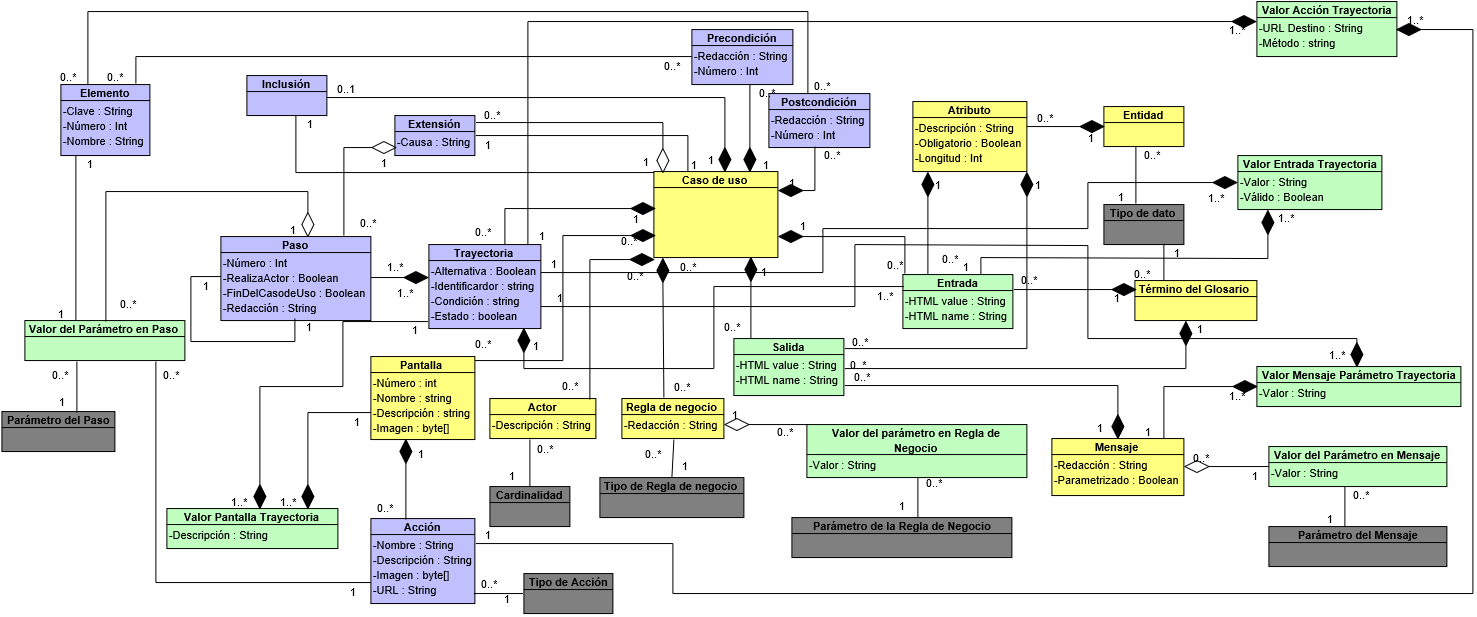
\includegraphics[angle=0,width=.95\textwidth]{images/modeloCasoUso}
		\caption{Modelo conceptual de casos de uso}
		\label{fig:modeloCasoUso}
	\end{center}
\end{figure}


\input{ModeloNegocio/Entidades/ModeloCasoUso/entidades/entidadCasoUso}
\input{ModeloNegocio/Entidades/ModeloCasoUso/entidades/entidadPantalla}
\input{ModeloNegocio/Entidades/ModeloCasoUso/entidades/entidadAccion}
\input{ModeloNegocio/Entidades/ModeloCasoUso/entidades/entidadActor}
\input{ModeloNegocio/Entidades/ModeloCasoUso/entidades/entidadTerminoGls}
\input{ModeloNegocio/Entidades/ModeloCasoUso/entidades/entidadBR}
\input{ModeloNegocio/Entidades/ModeloCasoUso/entidades/entidadMensaje}
\input{ModeloNegocio/Entidades/ModeloCasoUso/entidades/entidadAtributo}
\input{ModeloNegocio/Entidades/ModeloCasoUso/entidades/entidadEntidad}
\input{ModeloNegocio/Entidades/ModeloCasoUso/entidades/entidadTray}
\input{ModeloNegocio/Entidades/ModeloCasoUso/entidades/entidadPaso}
\input{ModeloNegocio/Entidades/ModeloCasoUso/entidades/entidadValorParametroPaso}
\input{ModeloNegocio/Entidades/ModeloCasoUso/entidades/entidadRevision}
\input{ModeloNegocio/Entidades/ModeloCasoUso/entidades/entidadExtension}
\input{ModeloNegocio/Entidades/ModeloCasoUso/entidades/entidadInclusion}
\input{ModeloNegocio/Entidades/ModeloCasoUso/entidades/entidadPrecondicion}
\input{ModeloNegocio/Entidades/ModeloCasoUso/entidades/entidadPostcondicion}

\section{Modelo Conceptual del Proyecto}
En la figura \ref{fig:modeloProyecto} se muestra la estructura de información que manejará el sistema para registrar proyectos y los colaboradores de la organización.

\begin{figure}[htbp!]
	\begin{center}
		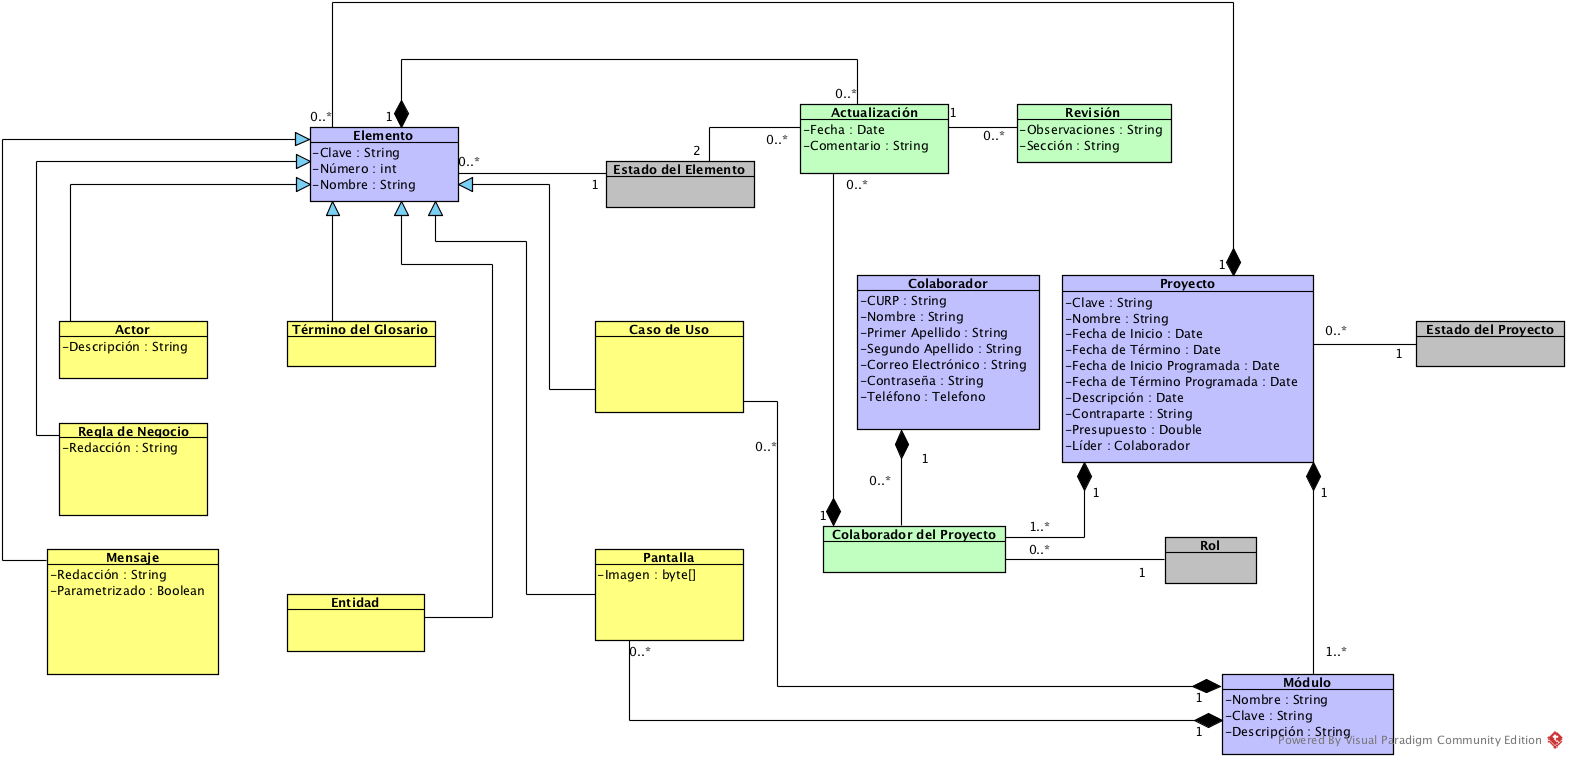
\includegraphics[angle=0,width=.95\textwidth]{images/modeloProyecto}
		\caption{Modelo conceptual de proyectos}
		\label{fig:modeloProyecto}
	\end{center}
\end{figure}

\input{ModeloNegocio/Entidades/ModeloProyecto/entidades/entidadElemento}
\input{ModeloNegocio/Entidades/ModeloProyecto/entidades/entidadProyecto}
\input{ModeloNegocio/Entidades/ModeloProyecto/entidades/entidadColaborador}
\input{ModeloNegocio/Entidades/ModeloProyecto/entidades/entidadColaboradorProyecto}
\input{ModeloNegocio/Entidades/ModeloProyecto/entidades/entidadModulo}
\input{ModeloNegocio/Entidades/ModeloProyecto/entidades/entidadActualizacion}
\input{ModeloNegocio/Entidades/ModeloProyecto/entidades/entidadRevision}
\section{Modelado de Reglas de negocio}


\begin{BussinesRule}{RN1}{Unicidad de números}
	\BRitem[Tipo:] Restricción de operación. 
	\BRitem[Clase:] Habilitadora. 
	\BRitem[Nivel:] Controla la operación. % Otras opciones para nivel: Control, Influencia.
	\BRitem[Descripción:] El número de los elementos del mismo tipo no pueden repetirse.
	\BRitem[Referenciado por:] \UCref{}{}.
\end{BussinesRule}


\begin{BussinesRule}{RN2}{Nombres de los elementos}
	\BRitem[Tipo:] Restricción de operación. 
	\BRitem[Clase:] Habilitadora. 
	\BRitem[Nivel:] Controla la operación. % Otras opciones para nivel: Control, Influencia.
	\BRitem[Descripción:] Los nombres de los elementos no pueden contener coma, punto, punto medio, dos puntos o guión bajo.
	\BRitem[Referenciado por:] \UCref{}{}.
\end{BussinesRule}


\begin{BussinesRule}{RN3}{Líder de análisis}
	\BRitem[Tipo:] Restricción de operación. 
	\BRitem[Clase:] Habilitadora. 
	\BRitem[Nivel:] Controla la operación. % Otras opciones para nivel: Control, Influencia.
	\BRitem[Descripción:] Los proyectos deben tener asignado solamente un líder de análisis.
	\BRitem[Referenciado por:] \UCref{}{}.
\end{BussinesRule}


\begin{BussinesRule}{RN5}{Modificación de elementos asociados a casos de uso liberados}
	\BRitem[Tipo:] Restricción de operación. 
	\BRitem[Clase:] Habilitadora. 
	\BRitem[Nivel:] Controla la operación. % Otras opciones para nivel: Control, Influencia.
	\BRitem[Descripción:] No es posible modificar entidades, reglas de negocio, actores, términos del glosario, pantallas y/o mensajes que se encuentren asociados a casos de uso con estado ''Liberado''.
	\BRitem[Referenciado por:] \UCref{}{}.
\end{BussinesRule}



\begin{BussinesRule}{RN6}{Unicidad de nombres}
	\BRitem[Tipo:] Restricción de operación. 
	\BRitem[Clase:] Habilitadora. 
	\BRitem[Nivel:] Controla la operación. % Otras opciones para nivel: Control, Influencia.
	\BRitem[Descripción:] El nombre de los elementos del mismo tipo no puede repetirse.
	\BRitem[Referenciado por:] \UCref{}{}.
\end{BussinesRule}

\begin{BussinesRule}{RN7}{Información correcta}
	\BRitem[Tipo:] Restricción de operación. 
	\BRitem[Clase:] Habilitadora. 
	\BRitem[Nivel:] Controla la operación. % Otras opciones para nivel: Control, Influencia.
	\BRitem[Descripción:]	Todos los datos proporcionados al sistema deben pertenecer al tipo de dato especificado en el modelo de información y respetar el formato con base en lo definido en la entidad del diccionario de datos.
	\BRitem[Referenciado por:] \UCref{CU1}{Iniciar Sesión}.
\end{BussinesRule}

\begin{BussinesRule}{RN8}{Datos Obligatorios} 
	\BRitem[Tipo:] Restricción de operación. 
	\BRitem[Clase:] Habilitadora. 
	\BRitem[Nivel:] Control. % Otras opciones para nivel: Control, Influencia.
	\BRitem[Descripción:] Los datos proporcionados al sistema que son marcados como requeridos con el carácter *,no se deben omitir.
	\BRitem[Referenciado por:] \UCref{CU1}{Iniciar Sesión}. 
\end{BussinesRule}



\begin{BussinesRule}{RN9}{Operaciones disponibles de casos de uso} 
	\BRitem[Tipo:] Restricción de operación. 
	\BRitem[Clase:] Habilitadora. 
	\BRitem[Nivel:] Control. % Otras opciones para nivel: Control, Influencia.
	\BRitem[Descripción:] Los estados de los casos de uso y el rol del actor determinan las operaciones que pueden solicitarse sobre un caso de uso desde la gestión:
	
	\begin{table}[H]
		\centering
		\begin{tabular}{|p{5cm}| p{5cm}| p{5cm}|}
			\hline
			\rowcolor{blue} \textcolor{white}{\textbf{Estado}} & \textcolor{white}{\textbf{Operaciones Analista}} & \textcolor{white}{\textbf{Operaciones Líder de Análisis}} \\
			\hline
			Edición & Consultar, editar, gestionar trayectorias, gestionar puntos de extensión, terminar y eliminar & Consultar, editar, gestionar trayectorias, gestionar puntos de extensión, terminar y eliminar \\
			\hline
			Revisión & Consultar y revisar & Consultar y revisar\\
			\hline
			Por liberar & Consultar & Consultar y Liberar\\
			\hline
			Pendiente de correción & Consultar, editar, gestionar trayectorias, gestionar puntos de extensión, terminar y eliminar & Consultar, editar, gestionar trayectorias, gestionar puntos de extensión, terminar y eliminar\\
			\hline
			Liberado & Consultar & Consultar, solicitar correciones\\
			\hline
			Configurado & Consultar & Consultar, solicitar correciones\\
			\hline
		\end{tabular}
	\end{table}

	\BRitem[Referenciado por:] \UCref{}{}.
	
\end{BussinesRule}
	
	\begin{BussinesRule}{RN10}{Referencias a elementos} 
		\BRitem[Tipo:] Restricción de operación. 
		\BRitem[Clase:] Habilitadora. 
		\BRitem[Nivel:] Control. % Otras opciones para nivel: Control, Influencia.
		\BRitem[Descripción:] Los elementos que podrán ser referenciados desde los casos de uso son aquellos que se encuentren registrados en el sistema.
		\BRitem[Referenciado por:] \UCref{}{}. 
	\end{BussinesRule} 


	\begin{BussinesRule}{RN11}{Registro de trayectorias} 
		\BRitem[Tipo:] Restricción de operación. 
		\BRitem[Clase:] Habilitadora. 
		\BRitem[Nivel:] Control. % Otras opciones para nivel: Control, Influencia.
		\BRitem[Descripción:] Al menos una de las trayectorias registradas debe ser marcada como principal.
		\BRitem[Referenciado por:] \UCref{}{}. 
	\end{BussinesRule}

\begin{BussinesRule}{RN12}{Identificador de elemento} 
	\BRitem[Tipo:] Restricción de operación. 
	\BRitem[Clase:] Habilitadora. 
	\BRitem[Nivel:] Control. % Otras opciones para nivel: Control, Influencia.
	\BRitem[Descripción:] El identificador de cada elemento se compone de un nombre, número y una clave. Donde el nombre es el que le asigna el usuario, el número es secuencial y la clave define el tipo de elemento: ''ENT'' para las entidades, ''ACT'' para los actores, ''CU'' para los casos de uso, ''IU'' para las pantallas, ''MSG'' para los mensajes, ''RN'' para las reglas de negocio y ''GLS'' para los términos del glosario.
	\BRitem[Referenciado por:] \UCref{}{}. 
\end{BussinesRule}

\begin{BussinesRule}{RN13}{Modificación del identificador} 
	\BRitem[Tipo:] Restricción de operación. 
	\BRitem[Clase:] Habilitadora. 
	\BRitem[Nivel:] Control. % Otras opciones para nivel: Control, Influencia.
	\BRitem[Descripción:] Una vez registrado un elemento no se podrá modificar el nombre, el número o la clave del identificador.
	\BRitem[Referenciado por:] \UCref{}{}. 
\end{BussinesRule}

\begin{BussinesRule}{RN14}{Salidas del casos de uso} 
	\BRitem[Tipo:] Restricción de operación. 
	\BRitem[Clase:] Habilitadora. 
	\BRitem[Nivel:] Control. % Otras opciones para nivel: Control, Influencia.
	\BRitem[Descripción:] En las salidas del caso de uso podrán enlistarse mensajes y atributos de las entidades.
	\BRitem[Referenciado por:] \UCref{}{}. 
\end{BussinesRule}

\begin{BussinesRule}{RN15}{Operaciones disponibles} 
	\BRitem[Tipo:] Restricción de operación. 
	\BRitem[Clase:] Habilitadora. 
	\BRitem[Nivel:] Control. % Otras opciones para nivel: Control, Influencia.
	\BRitem[Descripción:] Cuando una entidad, regla de negocio, actor, término del glosario, pantalla y/o mensaje, están en estado ''Edición'' es posible solicitar su consulta, modificación y eliminación. Cuando alguno de estos elementos se encuentre asociado a un caso de uso con estado ''Liberado'' solamente estará disponible la operación de consulta.
	\BRitem[Referenciado por:] \UCref{}{}. 
\end{BussinesRule}

\begin{BussinesRule}{RN16}{Nombres de las trayectorias} 
	\BRitem[Tipo:] Restricción de operación. 
	\BRitem[Clase:] Habilitadora. 
	\BRitem[Nivel:] Control. % Otras opciones para nivel: Control, Influencia.
	\BRitem[Descripción:] Los nombres de las trayectorias no pueden contener espacio, coma, punto, punto medio, dos puntos o guión bajo.
	\BRitem[Referenciado por:] \UCref{}{}. 
\end{BussinesRule}


\begin{BussinesRule}{RN17}{Unicidad de puntos de extensión} 
	\BRitem[Tipo:] Restricción de operación. 
	\BRitem[Clase:] Habilitadora. 
	\BRitem[Nivel:] Control. % Otras opciones para nivel: Control, Influencia.
	\BRitem[Descripción:] No puede existir más de un punto de extensión con el mismo caso de uso origen y el mismo caso de uso destino.
	\BRitem[Referenciado por:] \UCref{}{}. 
\end{BussinesRule}


\begin{BussinesRule}{RN18}{Eliminación de elemento} 
	\BRitem[Tipo:] Restricción de operación. 
	\BRitem[Clase:] Habilitadora. 
	\BRitem[Nivel:] Control. % Otras opciones para nivel: Control, Influencia.
	\BRitem[Descripción:] No es posible eliminar entidades, reglas de negocio, actores, términos del glosario, pantallas y/o mensajes que se encuentren asociados a casos de uso con estado ''Liberado''.
	\BRitem[Referenciado por:] \UCref{}{}. 
\end{BussinesRule}

\begin{BussinesRule}{RN19}{Formato de correo electrónico} 
	\BRitem[Tipo:] Restricción de operación. 
	\BRitem[Clase:] Habilitadora. 
	\BRitem[Nivel:] Control. % Otras opciones para nivel: Control, Influencia.
	\BRitem[Descripción:] El correo electrónico debe ser una cadena de caracteres con la siguiente estructura ordenada:
	\begin{enumerate}
		\item Cadena de caracteres
		\item ''@''
		\item Cadena de caracteres
		\item ''.''
		\item Cadena de caracteres
	\end{enumerate}
	\BRitem[Ejemplo]: cadena1@cadena2.cadena3
	\BRitem[Referenciado por:] \UCref{}{}. 
\end{BussinesRule}

\begin{BussinesRule}{RN20}{Verificación de catálogos} 
	\BRitem[Tipo:] Restricción de operación. 
	\BRitem[Clase:] Habilitadora. 
	\BRitem[Nivel:] Control. % Otras opciones para nivel: Control, Influencia.
	\BRitem[Descripción:] Es necesario que exista información registrada en los catálogos al momento de solicitar una operación que requiera de estos.
	\BRitem[Referenciado por:] \UCref{}{}. 
\end{BussinesRule}


\begin{BussinesRule}{RN21}{Estados para iniciar un proyecto} 
	\BRitem[Tipo:] Restricción de operación. 
	\BRitem[Clase:] Habilitadora. 
	\BRitem[Nivel:] Control. % Otras opciones para nivel: Control, Influencia.
	\BRitem[Descripción:] Se podrán registrar proyectos con estado ''En Negociación'' o ''Iniciado''.
	\BRitem[Referenciado por:] \UCref{}{}. 
\end{BussinesRule}

\begin{BussinesRule}{RN22}{Unicidad de la clave del proyecto} 
	\BRitem[Tipo:] Restricción de operación. 
	\BRitem[Clase:] Habilitadora. 
	\BRitem[Nivel:] Control. % Otras opciones para nivel: Control, Influencia.
	\BRitem[Descripción:] La clave de los proyectos debe ser única en todo el sistema.
	\BRitem[Referenciado por:] \UCref{}{}. 
\end{BussinesRule}

\begin{BussinesRule}{RN23}{Unicidad de la clave del módulo} 
	\BRitem[Tipo:] Restricción de operación. 
	\BRitem[Clase:] Habilitadora. 
	\BRitem[Nivel:] Control. % Otras opciones para nivel: Control, Influencia.
	\BRitem[Descripción:] La clave de los módulos debe ser única en un proyecto.
	\BRitem[Referenciado por:] \UCref{}{}. 
\end{BussinesRule}

\begin{BussinesRule}{RN24}{Unicidad de la clave de la trayectoria} 
	\BRitem[Tipo:] Restricción de operación. 
	\BRitem[Clase:] Habilitadora. 
	\BRitem[Nivel:] Control. % Otras opciones para nivel: Control, Influencia.
	\BRitem[Descripción:] La clave de las trayectorias debe ser única en un caso de uso.
	\BRitem[Referenciado por:] \UCref{}{}. 
\end{BussinesRule}

\begin{BussinesRule}{RN25}{Relación entre fechas del proyecto} 
	\BRitem[Tipo:] Restricción de operación. 
	\BRitem[Clase:] Habilitadora. 
	\BRitem[Nivel:] Control. % Otras opciones para nivel: Control, Influencia.
	\BRitem[Descripción:] La fecha de término del proyecto debe ser posterior a la fecha de inicio.
	\BRitem[Referenciado por:] \UCref{}{}. 
\end{BussinesRule}

\begin{BussinesRule}{RN26}{Relación entre fechas programadas del proyecto} 
	\BRitem[Tipo:] Restricción de operación. 
	\BRitem[Clase:] Habilitadora. 
	\BRitem[Nivel:] Control. % Otras opciones para nivel: Control, Influencia.
	\BRitem[Descripción:] La fecha de término programada del proyecto debe ser posterior a la fecha de inicio programada.
	\BRitem[Referenciado por:] \UCref{}{}. 
\end{BussinesRule}

\begin{BussinesRule}{RN27}{Eliminación de personas} 
	\BRitem[Tipo:] Restricción de operación. 
	\BRitem[Clase:] Habilitadora. 
	\BRitem[Nivel:] Control. % Otras opciones para nivel: Control, Influencia.
	\BRitem[Descripción:] No es posible eliminar una persona, si esta es líder de al menos un proyecto.
	\BRitem[Referenciado por:] \UCref{}{}. 
\end{BussinesRule}

\begin{BussinesRule}{RN28}{Eliminación de módulos} 
	\BRitem[Tipo:] Restricción de operación. 
	\BRitem[Clase:] Habilitadora. 
	\BRitem[Nivel:] Control. % Otras opciones para nivel: Control, Influencia.
	\BRitem[Descripción:] No es posible eliminar un módulo, si algún elemento de otro módulo, tiene referencias a al menos un elemento del módulo que desea eliminarse.
	\BRitem[Referenciado por:] \UCref{}{}. 
\end{BussinesRule}

\begin{BussinesRule}{RN29}{Unicidad de casos de uso} 
	\BRitem[Tipo:] Restricción de operación. 
	\BRitem[Clase:] Habilitadora. 
	\BRitem[Nivel:] Control. % Otras opciones para nivel: Control, Influencia.
	\BRitem[Descripción:] Diferentes casos de uso pueden tener el mismo nombre y/o número, únicamente si cada uno de estos pertenecen a diferentes módulos.
	\BRitem[Referenciado por:] \UCref{}{}. 
\end{BussinesRule}

\begin{BussinesRule}{RN30}{Unicidad de pantallas} 
	\BRitem[Tipo:] Restricción de operación. 
	\BRitem[Clase:] Habilitadora. 
	\BRitem[Nivel:] Control. % Otras opciones para nivel: Control, Influencia.
	\BRitem[Descripción:] Diferentes pantallas pueden tener el mismo nombre y/o número, únicamente si cada una de estas pertenecen a diferentes módulos.
	\BRitem[Referenciado por:] \UCref{}{}. 
\end{BussinesRule}

\begin{BussinesRule}{RN31}{Estructura de tokens} 
	\BRitem[Tipo:] Restricción de operación. 
	\BRitem[Clase:] Habilitadora. 
	\BRitem[Nivel:] Control. % Otras opciones para nivel: Control, Influencia.
	\BRitem[Descripción:] Los tokens utilizados para referenciar elementos deben mantener una estructura determinada de acuerdo al tipo de elemento referenciado:
	\begin{itemize}
		\item Regla de negocio: {\em RN·Número:Nombre}
		\begin{itemize}
			\item ''RN'': cadena que indica que el tipo de elemento referenciado es una regla de negocio.
			\item ''·'': símbolo para separar las partes del token (punto medio).
			\item ''Número'': número de la regla de negocio referenciada.
			\item '':'': símbolo para separar las partes del token (dos puntos).
			\item ''Nombre'': nombre de la regla de negocio referenciada.
		\end{itemize}
		\item Entidad: {\em ENT·Nombre}
		\begin{itemize}
			\item ''ENT'': cadena que indica que el tipo de elemento referenciado es una entidad.
			\item ''·'': símbolo para separar las partes del token (punto medio).
			\item ''Nombre'': nombre de la entidad referenciada.
		\end{itemize}
		\item Caso de uso: {\em CU·ClaveMódulo·Número:Nombre}
		\begin{itemize}
			\item ''CU'': cadena que indica que el tipo de elemento referenciado es un caso de uso.
			\item ''·'': símbolo para separar las partes del token (punto medio).
			\item ''ClaveMódulo'': clave del módulo a la que pertenece el caso de uso referenciado.
			\item ''Número'': número del caso de uso referenciado.
			\item '':'': símbolo para separar las partes del token (dos puntos).
			\item ''Nombre'': nombre del caso de uso referenciado.
		\end{itemize}
		\item Pantalla: {\em IU·ClaveMódulo·Número:Nombre}
		\begin{itemize}
			\item ''IU'': cadena que indica que el tipo de elemento referenciado es una pantalla.
			\item ''·'': símbolo para separar las partes del token (punto medio).
			\item ''ClaveMódulo'': clave del módulo a la que pertenece la pantalla referenciada.
			\item ''Número'': número de la pantalla referenciada.
			\item '':'': símbolo para separar las partes del token (dos puntos).
			\item ''Nombre'': nombre de la pantalla referenciada.
		\end{itemize}
		\item Mensaje: {\em MSG·Número:Nombre}
		\begin{itemize}
			\item ''MSG'': cadena que indica que el tipo de elemento referenciado es un mensaje.
			\item ''·'':  símbolo para separar las partes del token (punto medio).
			\item ''Número'': número del mensaje referenciado.
			\item '':'': símbolo para separar las partes del token (dos puntos).
			\item ''Nombre'': nombre del mensaje referenciado.
		\end{itemize}
	\item Actor: {\em ACT·Nombre}
		\begin{itemize}
			\item ''ACT'': cadena que indica que el tipo de elemento referenciado es un actor.
			\item ''·'':  símbolo para separar las partes del token (punto medio).
			\item ''Nombre'': nombre del actor referenciado.
		\end{itemize}
	\item Término de glosario: {\em GLS·Nombre}
		\begin{itemize}
			\item ''GLS'': cadena que indica que el tipo de elemento referenciado es un témino del glosario.
			\item ''·'':  símbolo para separar las partes del token (punto medio).
			\item ''Nombre'': nombre del término del glosario referenciado.
		\end{itemize}
	\item Atributo: {\em ATR·Entidad:Nombre}
		\begin{itemize}
			\item ''ATR'': cadena que indica que el tipo de elemento referenciado es un atributo.
			\item ''·'':  símbolo para separar las partes del token (punto medio).
			\item ''Entidad'': nombre de la entidad a la que pertenece el atributo referenciado.
			\item '':'': símbolo para separar las partes del token (dos puntos).
			\item ''Nombre'': nombre del atributo referenciado.
		\end{itemize}
	\item Trayectoria: {\em TRAY·ClaveCasoUso·NúmeroCasoUso:NombreCasoUso:Clave}
		\begin{itemize}
			\item ''TRAY'': cadena que indica que el tipo de elemento referenciado es una trayectoria.
			\item ''·'':  símbolo para separar las partes del token (punto medio).
			\item ''ClaveCasoUso'': clave del caso de uso al que pertenece la trayectoria referenciada.
			\item ''NúmeroCasoUso'': número del caso de uso al que pertenece la trayectoria referenciada.
			\item '':'': símbolo para separar las partes del token (dos puntos).
			\item ''NombreCasoUso'': nombre del caso de uso al que pertenece la trayectoria referenciada.
			\item ''Clave'': clave de la trayectoria referenciada.
		\end{itemize}
	\item Paso: {\em P·ClaveCasoUso·NúmeroCasoUso:NombreCasoUso:ClaveTrayectoria·Número}
		\begin{itemize}
			\item ''P'': cadena que indica que el tipo de elemento referenciado es un paso.
			\item ''·'':  símbolo para separar las partes del token (punto medio).
			\item ''ClaveCasoUso'': clave del caso de uso al que pertenece el paso referenciado.
			\item ''NúmeroCasoUso'': número del caso de uso al que pertenece el paso referenciado.
			\item '':'': símbolo para separar las partes del token (dos puntos).
			\item ''NombreCasoUso'': nombre del caso de uso al que pertenece el paso referenciado.
			\item ''ClaveTrayectoria'': clave de la trayectoria a la que pertenece el paso referenciado.
			\item ''Número'': número del paso referenciado.
		\end{itemize}
	\item Acción: {\em ACC·ClavePantalla·NúmeroPantalla:NombrePantalla:Nombre}
		\begin{itemize}
			\item ''ACC'': cadena que indica que el tipo de elemento referenciado es una acción.
			\item ''·'':  símbolo para separar las partes del token (punto medio).
			\item ''ClavePantalla'': clave de la pantalla a la que pertenece la acción referenciada.
			\item ''NúmeroPantalla'': número de la pantalla a la que pertenece la acción referenciada.
			\item '':'': símbolo para separar las partes del token (dos puntos).
			\item ''NombrePantalla'': nombre de la pantalla a la que pertenece la acción referenciada.
			\item ''Nombre'': nombre de la acción referenciada.
		\end{itemize}
	\item Parámetro (Mensajes): {\em PARAM·Nombre}
		\begin{itemize}
			\item ''PARAM'': cadena que indica que se está realizando una referencia a un parámetro en un mensaje.
			\item ''·'':  símbolo para separar las partes del token (punto medio).
			\item ''Nombre'': nombre del parámentro referenciado.
		\end{itemize}
	\end{itemize}
	\BRitem[Referenciado por:] \UCref{}{}. 
\end{BussinesRule}


\begin{BussinesRule}{RN32}{Pasos en la trayectoria} 
	\BRitem[Tipo:] Restricción de operación. 
	\BRitem[Clase:] Habilitadora. 
	\BRitem[Nivel:] Control. % Otras opciones para nivel: Control, Influencia.
	\BRitem[Descripción:] Una trayectoria debe debe contar al menos con un paso.
	\BRitem[Referenciado por:] \UCref{}{}. 
\end{BussinesRule}

\begin{BussinesRule}{RN33}{Longitud de la CURP} 
	\BRitem[Tipo:] Restricción de operación. 
	\BRitem[Clase:] Habilitadora. 
	\BRitem[Nivel:] Control. % Otras opciones para nivel: Control, Influencia.
	\BRitem[Descripción:] La CURP de un colaborador debe tener exactamente 18 caracteres alfanuméricos.
	\BRitem[Referenciado por:] \UCref{}{}. 
\end{BussinesRule}


\begin{BussinesRule}{RN34}{Eliminación de proyectos} 
	\BRitem[Tipo:] Restricción de operación. 
	\BRitem[Clase:] Habilitadora. 
	\BRitem[Nivel:] Control. % Otras opciones para nivel: Control, Influencia.
	\BRitem[Descripción:] No es posible eliminar un proyecto, si este tiene elementos asociados.
	\BRitem[Referenciado por:] \UCref{}{}. 
\end{BussinesRule}


\begin{BussinesRule}{RN35}{Validar Fecha} 
	\BRitem[Tipo:] Restricción de operación. 
	\BRitem[Clase:] Habilitadora. 
	\BRitem[Nivel:] Control. % Otras opciones para nivel: Control, Influencia.
	\BRitem[Descripción:] Para registrar la duración de un proyecto, la fecha de termino programada debe ser posterior a la fecha de inicio programada.
	\BRitem[Referenciado por:] \UCref{}{}. 
\end{BussinesRule}

%---------------------------------------------------------


%----------------------------------------------------------

%---------------------------------------------------------


%=========================================================
%=========================================================
%\chapter{Modelo de comportamiento}	
%\label{cap:modDinamico}

%	En este capítulo se describen los actores que interactúan con el sistema, así como los casos de uso de las operaciones más representativas.
	
%\begin{figure}[htbp]
%	\begin{center}
%		\fbox{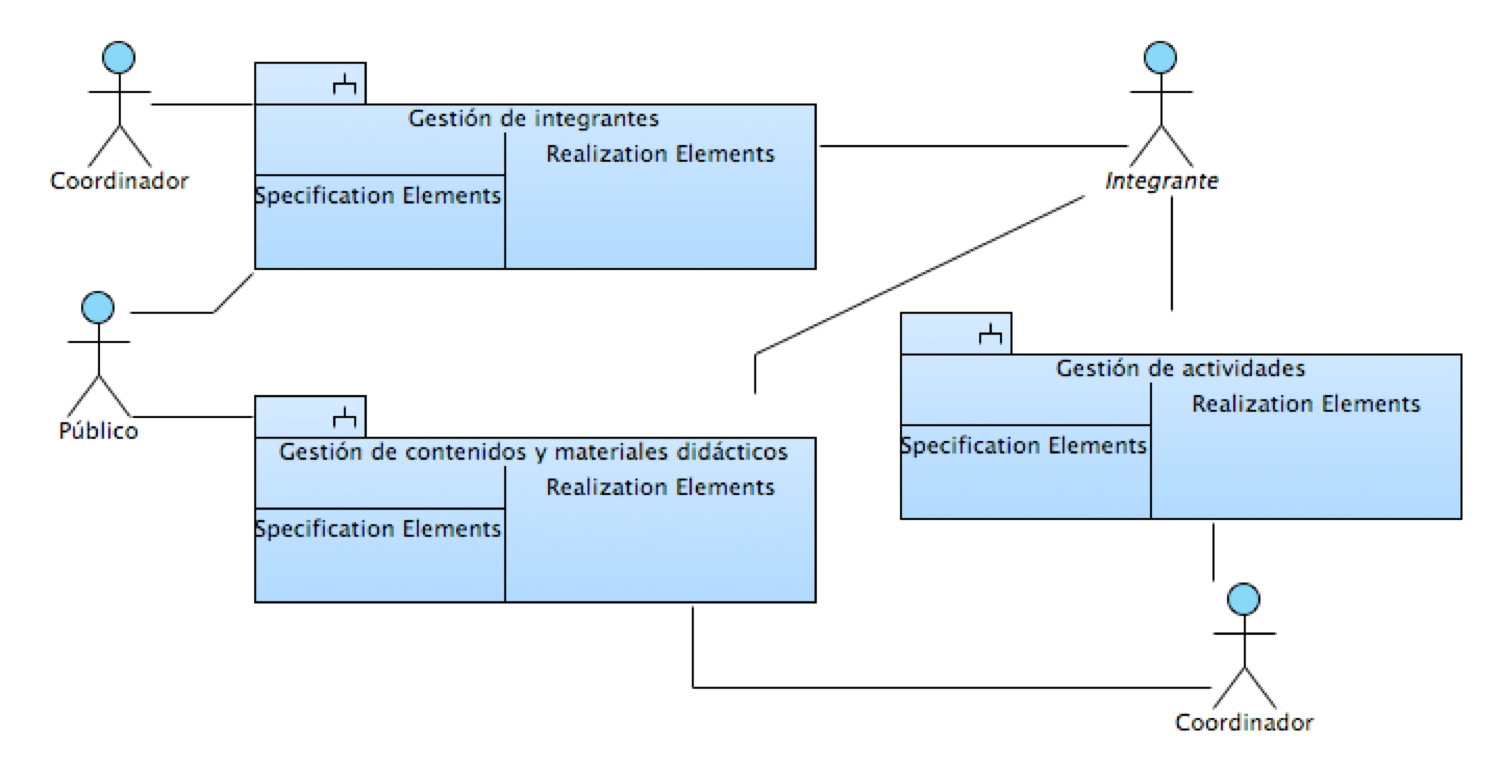
\includegraphics[width=.8\textwidth]{images/casosDeUso}}
%		\caption{Diagrama de casos de uso del sistema. (Hacer y cambiar los diagramas}
%		\label{fig:casosDeUso}
%	\end{center}
%\end{figure}

%\begin{figure}[htbp]
%	\begin{center}
%		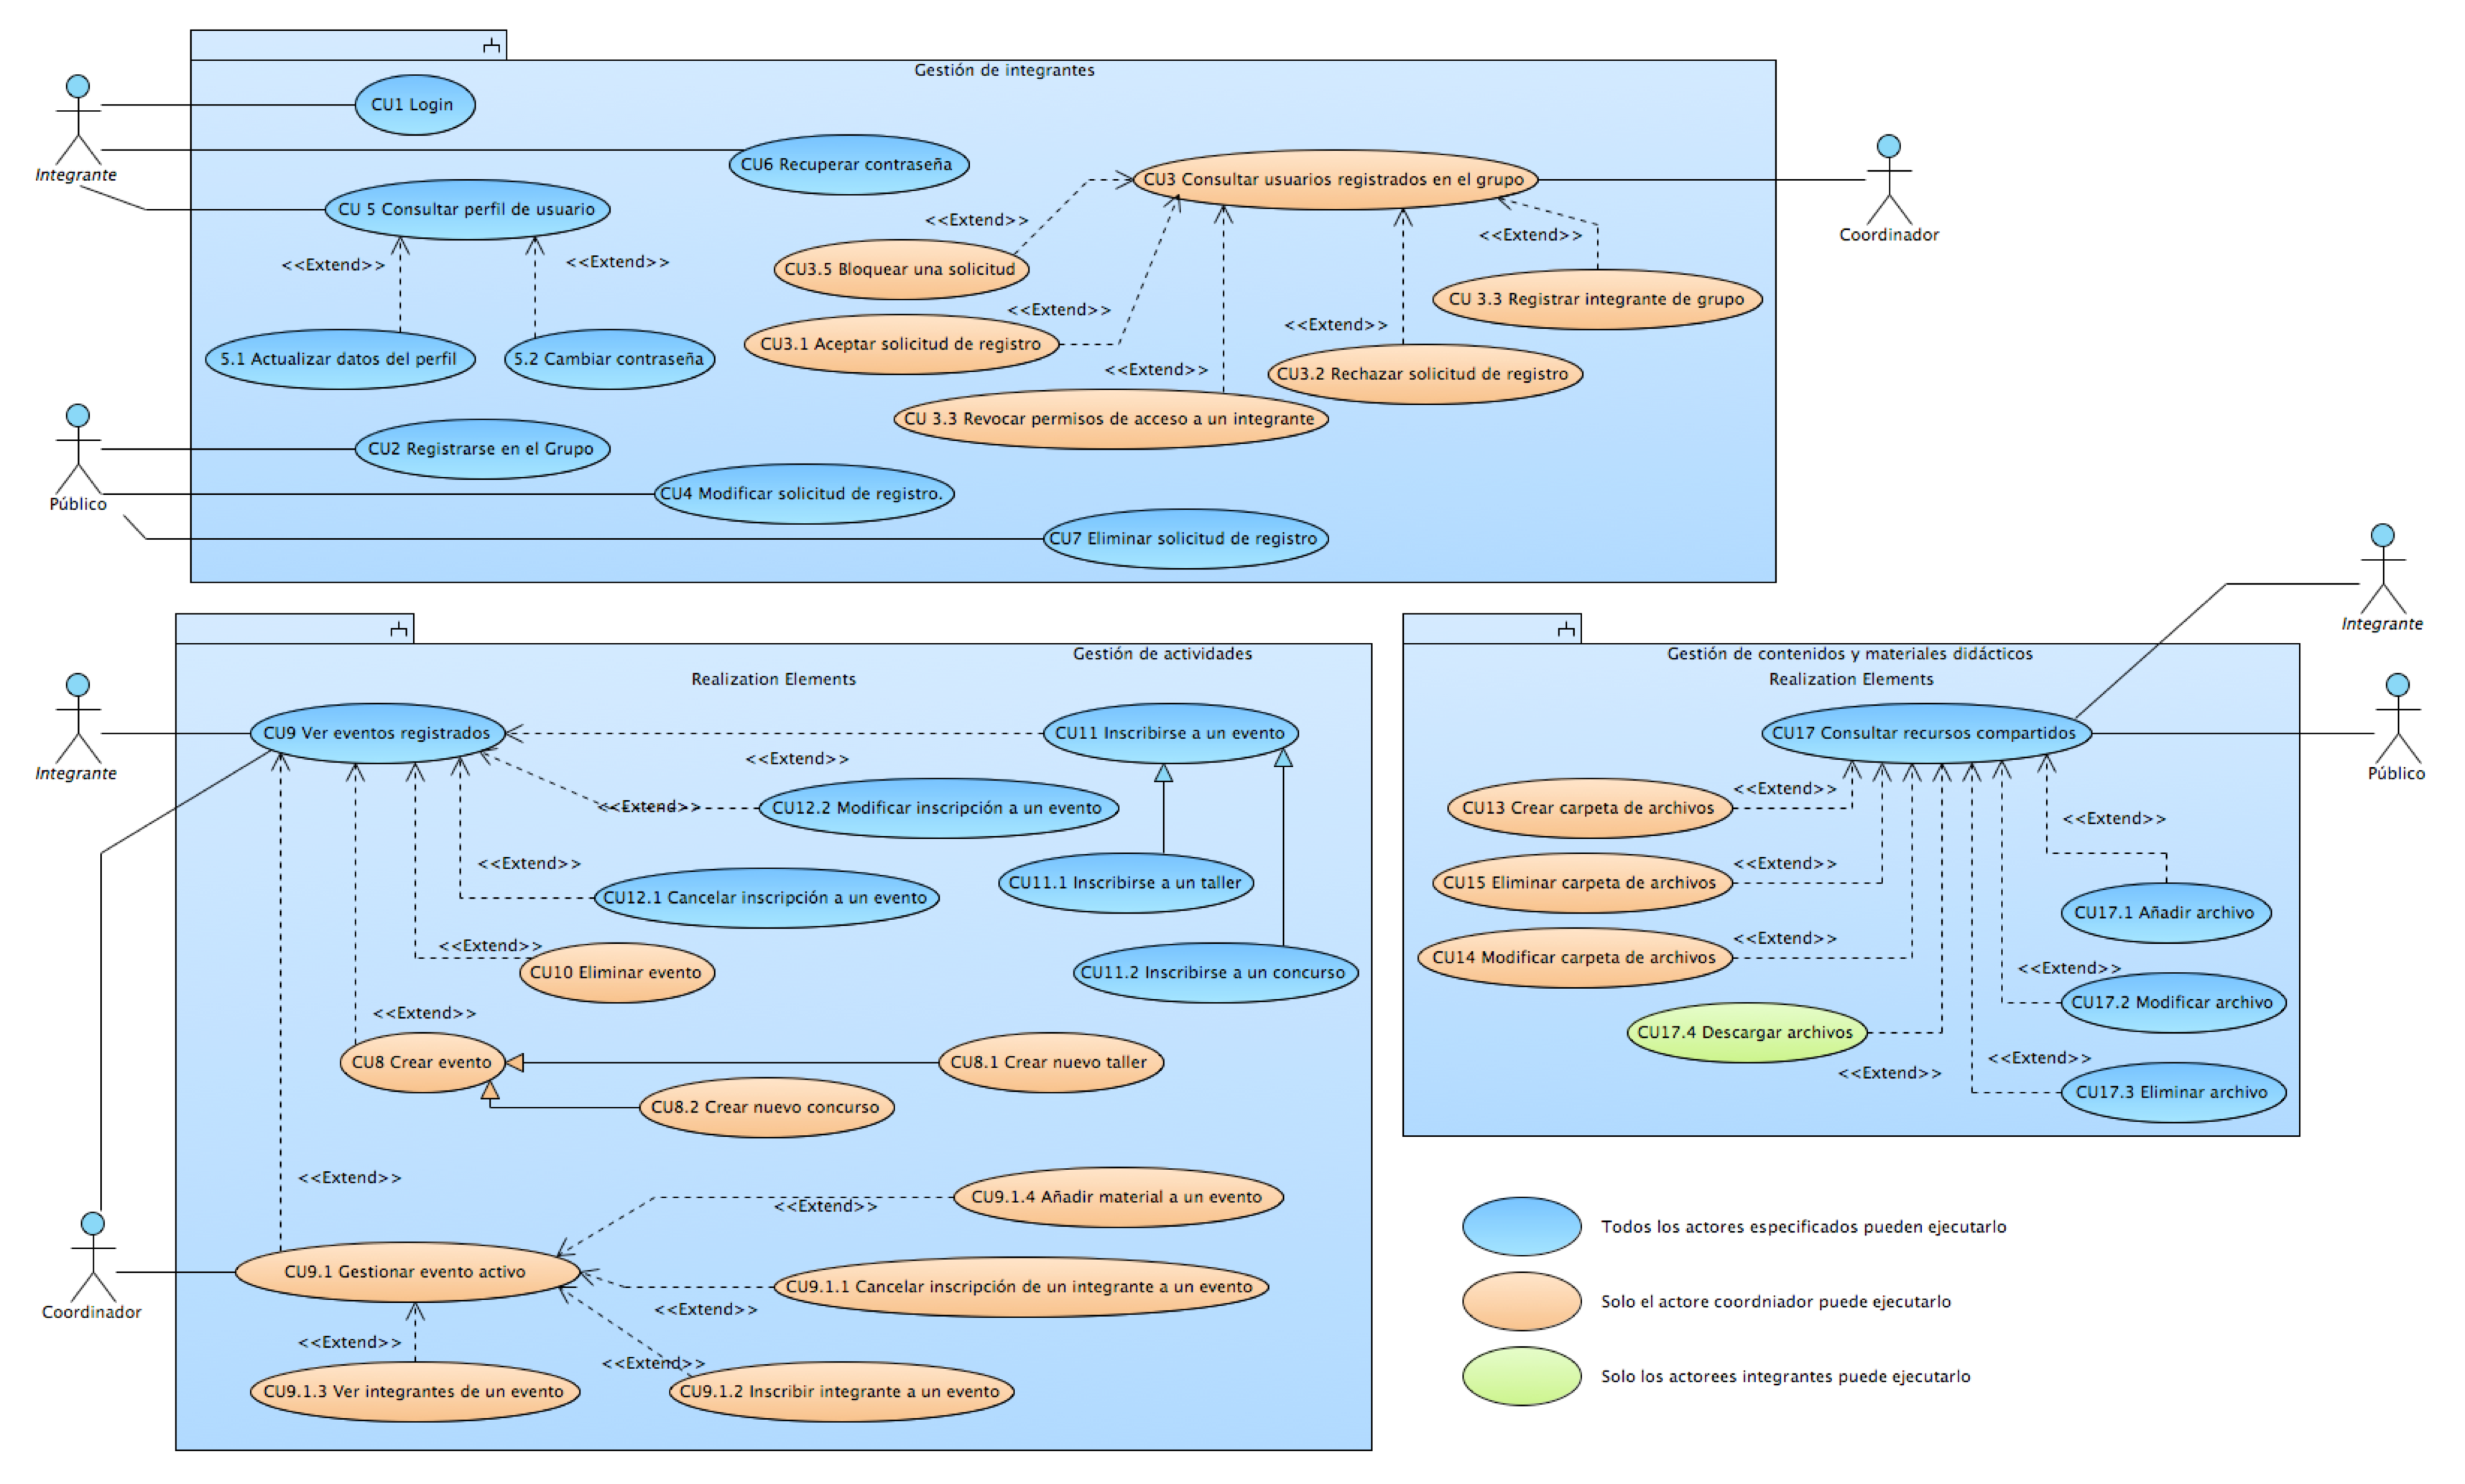
\includegraphics[angle=90, width=.7\textwidth]{images/casosDeUsoDetalle}
%		\caption{Diagrama detallado del sistema.}
%		\label{fig:casosDeUsoDetalle}
%	\end{center}
%\end{figure}

%---------------------------------------------------------
\section{Modelo de actores}
Los actores del sistema son los perfiles que tienen un usuario que interactúa con el sistema. Los perfiles que puede tener un usuario son: administrador, líder de análisis y el analista.
%---------------------------------------------------------
\begin{Usuario}{\hypertarget{admin}{\subsection{Administrador}}}{
}
	\item[Descripción: ]
	Es la persona encargada de registrar los proyectos y al personal de la organización.
    \item[Responsabilidades:] \cdtEmpty
    \begin{itemize}
		\item Registrar y modificar la información de los proyectos.
		\item Asignar un líder de análisis a los proyectos.
		\item Registrar y modificar la información
    \end{itemize}

	\item[Perfil:] \cdtEmpty
    \begin{itemize}
		\item Debe conocer los proyectos que la organización va a comenzar.
		\item Debe conocer toda la información del personal que colabora en la organización.
    \end{itemize}
    
    \item[Cantidad: ]
    Uno.
\end{Usuario}

\begin{Usuario}{\hypertarget{jefe}{\subsection{Líder de proyecto}}}{
}
	\item[Descripción:]
	Es la persona encargada de dirigir y coordinar el proyecto en desarrollo.
    \item[Responsabilidades:] \cdtEmpty
    \begin{itemize}
		\item Asignar los colaboradores del proyecto que dirige.
		\item Registrar y modificar módulos para los casos de uso y pantallas.
		\item Registrar y modificar los elementos del sistema.
		\item Revisar y realizar observaciones de los elementos para enviarlos a corrección.
		\item Liberar los casos de uso que considere completos y correctos.
    \end{itemize}

	\item[Perfil:] \cdtEmpty
    \begin{itemize}
		\item Debe tener conocimientos referentes a la documentación de sistemas.
		\item Debe tener dominio de Organización de equipos de desarrollo de software, estructuración de equipo, distribución de tareas y administración del tiempo.
		\item Debe tener conocimientos de planificación de tiempo, estimación de costos, estimación de proyectos y estimación de riesgos.
    \end{itemize}
    \item[Cantidad: ]
    Uno por proyecto.
\end{Usuario}


\begin{Usuario}{\hypertarget{analista}{\subsection{Analista}}}{
}
	\item[Descripción:]
	Es la persona encargada de documentar los elementos que componen el proyecto y validar los requerimientos del software.
    \item[Responsabilidades:] \cdtEmpty
    \begin{itemize}
		\item Registrar y modificar módulos para los casos de uso y pantallas 
		\item Registrar y modificar los elementos del sistema.
		\item Corregir la información de los elementos con base a las observaciones realizadas por el líder de análisis.
    \end{itemize}

	\item[Perfil:] \cdtEmpty
    \begin{itemize}
		\item Debe tener conocimientos referentes a la documentación de sistemas.
		\item Debe tener habilidad para comunicarse de manera efectiva con los demás colaboradores del proyecto.
    \end{itemize}
    \item[Cantidad: ]
    De acuerdo al personal de la organización.
\end{Usuario}
%Casos de uso%
\section{Casos de uso}
Los casos de uso que describen el funcionamiento del prototipo se muestran en la figura 3.1 Casos de uso del editor, los casos de uso se dividieron por módulos para organizar de una mejor manera la visualización y el desarrollo. Los módulos que conforman el editor son:

\begin{itemize}
	\item Administrador
	\item Líder de Análisis
	\item Módulos
	\item Casos de Uso
	\item Pantallas
	\item Entidades
	\item Reglas de Negocio
	\item Mensajes
	\item Actores
	\item Términos del Glosario
\end{itemize}

	\begin{UseCase}{CU1}{Iniciar sesión}{
		El actor se ingresa con su nombre y contraseña a su perfil y hacer uso de las funciones que le competen.
	}
		\UCitem{Versión}{\color{Gray}0.1}
		\UCitem{Actor}{\hyperlink{jefe}{Líder de proyecto}, \hyperlink{analista}{Analista}, \hyperlink{admin}{Administrador}}
		\UCitem{Propósito}{Iniciar sesión en el sistema.}
		\UCitem{Entradas}{\begin{itemize}
				\item \cdtRef{colaboradorEntidad:correoColaborador}{Correo}: Se escribe desde el teclado
				\item \cdtRef{colaboradorEntidad:passColaborador}{Contraseña}: Se escribe desde el teclado
		\end{itemize}}
		\UCitem{Salidas}{Ninguna}
		\UCitem{Destino}{Pantalla}
		\UCitem{Precondiciones}{Que el actor se encuentre registrado en el sistema.}
		\UCitem{Postcondiciones}{El actor podrá hacer uso del sistema.}
		\UCitem{Errores}{\begin{itemize}
		\item \cdtIdRef{MSG4}{Dato Obligatorio}: Se muestra en la pantalla \IUref{IU1}{Iniciar Sesión} cuando no se ha ingresado un dato marcado como obligatorio.
		\item \cdtIdRef{MSG6}{Longitud inválida}: Se muestra en la pantalla \IUref{IU1}{Iniciar Sesión} cuando se ha excedido la longitud de alguno de los campos.
		\item \cdtIdRef{MSG23}{Correo electrónico y/o contraseña incorrectos}: Se muestra en la pantalla \IUref{IU1}{Iniciar Sesión} cuando el correo electrónico y/o la contraseña ingresada son incorrectos.
		\item \cdtIdRef{MSG31}{Longitud Mínima}: Se muestra en la pantalla \IUref{IU1}{Iniciar Sesión} cuando se ha ingresado una contraseña que no cumple con la longitud mínima.
		\end{itemize}
		}
		\UCitem{Tipo}{Caso de uso primario}
	\end{UseCase}
%--------------------------------------
	\begin{UCtrayectoria}
		\UCpaso[\UCactor] Solicita ingresar al sistema a través de la URL.
		\UCpaso[\UCsist] Muestra la pantalla \IUref{IU1}{Iniciar Sesión}.
		\UCpaso[\UCactor] Ingresa los datos solicitados. \label{P3}
		\UCpaso[\UCactor] Oprime el botón \IUbutton{Aceptar}.
		\UCpaso[\UCsist] Verifica que no se haya omitido ningún campo marcado como obligatorio con base en la regla de negocio \BRref{RN8}{Datos Obligatorios}. \hyperlink{CU1:TAA}{[Trayectoria alternativa A]}
		\UCpaso[\UCsist] Verifica que los datos cumplan con el formato y el tipo de dato requerido, con base en la regla de negocio \BRref{RN7}{Información correcta}. \Trayref{B} \Trayref{C} \Trayref{D}
		\UCpaso[\UCsist] Verifica que el actor se encuentre registrado en el sistema. \Trayref{E}
		\UCpaso[\UCsist] Verifica que la contraseña ingresada corresponda con la del usuario. \Trayref{E}
		\UCpaso[\UCsist] Muestra la pantalla IU 4 Gestionar proyectos.	
	\end{UCtrayectoria}		
%--------------------------------------
		\hypertarget{CU1:TAA}{\textbf{Trayectoria alternativa A}}\\
		\noindent \textbf{Condición:} El actor no ingresó uno o más campos obligatorios
		\begin{enumerate}
			\UCpaso[\UCsist] Muestra el mensaje \cdtIdRef{MSG4}{Dato Obligatorio} y señala el campo que presenta el error en la pantalla \IUref{IU1}{Iniciar Sesión}.
			\UCpaso[\UCactor] Regresa al paso \ref{P3} de la Trayectoria Principal.
			\item[- -] - - {\em {Fin de la trayectoria}}.%
		\end{enumerate}

%--------------------------------------
		\begin{UCtrayectoriaA}{B}{El actor ingresó un dato con un número de caracteres fuera del rango permitido}
	\UCpaso[\UCsist] Muestra el \cdtIdRef{MSG6}{Longitud inválida} y señala el campo que presenta el error en la pantalla \IUref{IU1}{Iniciar Sesión}.
	\UCpaso[\UCactor] Regresa al paso \ref{P3} de la Trayectoria Principal.
\end{UCtrayectoriaA}

	\begin{UCtrayectoriaA}{C}{El actor ingresó un tipo de dato incorrecto.}
		\UCpaso[\UCsist] Muestra el mensaje \cdtIdRef{MSG29}{Formato incorrecto} y señala el campo que presenta el dato inválido en la pantalla \IUref{IU1}{Iniciar sesión}, para indicar que se ha ingresado un tipo de dato inválido.
		\UCpaso Regresa al paso \ref{P3} de la trayectoria principal.
	\end{UCtrayectoriaA}

	\begin{UCtrayectoriaA}{D}{El actor ingresó una contraseña que no cumple la longitud mínima requerida}
		\UCpaso[\UCsist] Muestra el mensaje \cdtIdRef{MSG31}{Longitud mínima} y señala el campo que presenta el dato inválido en la pantalla \IUref{IU1}{Iniciar sesión}, para indicar que se ha ingresado una contraseña que no cumple con la longitud mínima.
		\UCpaso Regresa al paso \ref{P3} de la trayectoria principal.
	\end{UCtrayectoriaA}
%--------------------------------------
		\begin{UCtrayectoriaA}{E}{El actor ingresó un dato incorrecto}
	\UCpaso[\UCsist] Muestra el mensaje \cdtIdRef{MSG23}{Correo electrónico y/o contraseña incorrectos} en la pantalla \IUref{IU1}{Iniciar Sesión} notificando que los datos ingresados son incorrectos.
	\UCpaso[\UCactor] Regresa al paso \ref{P3} de la Trayectoria Principal.
\end{UCtrayectoriaA}
	\begin{UseCase}{CU2}{Gestionar proyectos de Administrador}{
		Permite al Administrador visualizar todos los proyectos registrados en el sistema, además sirve como punto de acceso para registrar, modificar o eliminar un proyecto.
	}
		\UCitem{Versión}{\color{Gray}0.1}
		\UCitem{Actor}{\hyperlink{admin}{Administrador}}
		\UCitem{Propósito}{Proporcionar al actor un mecanismo para llevar el control de los proyectos.}
		\UCitem{Entradas}{Ninguna}
		\UCitem{Salidas}{\begin{itemize}
				\item \hyperlink{proyectoEntidad}{Proyecto}: Tabla que muestra la \cdtRef{proyectoEntidad:claveProyecto}{clave}, \cdtRef{proyectoEntidad:nombreProyecto}{nombre} y el \cdtRef{proyectoEntidad:liderProyecto}{Líder de Proyecto} de todos los proyectos existentes.
		\end{itemize}}
		\UCitem{Destino}{Pantalla}
		\UCitem{Precondiciones}{Ninguna}
		\UCitem{Postcondiciones}{Ninguna}
		\UCitem{Errores}{\begin{itemize}
		\item \cdtIdRef{MSG2}{No existe información}: Se muestra en la pantalla \IUref{IU2}{Gestionar proyectos de Administrador} cuando no existen proyectos registrados
		\end{itemize}
		}
		\UCitem{Tipo}{Caso de uso primario}
	\end{UseCase}
%--------------------------------------
	\begin{UCtrayectoria}
		\UCpaso[\UCactor] Solicita gestionar los proyectos presionando la opción ''Proyectos'' del menú \IUref{MN1}{Menú de Administrador}.
		\UCpaso[\UCsist] Busca la información de los proyectos registrados. \hyperlink{CU2:TAA}{[Trayectoria A]}
		\UCpaso[\UCsist] Muestra la información de los proyectos en la pantalla \IUref{IU2}{Gestionar proyectos de Administrador}.
		\UCpaso[\UCactor] Gestiona los proyectos a través de los botones: \IUbutton{Registrar}, \editar  y \eliminar. \label{P4}
	\end{UCtrayectoria}		
%--------------------------------------
	\hypertarget{CU2:TAA}{\textbf{Trayectoria alternativa A}}\\
\noindent \textbf{Condición:} No existen registros de proyectos.
\begin{enumerate}
	\UCpaso[\UCsist] Muestra el mensaje \cdtIdRef{MSG2}{No existe información} en la pantalla \IUref{IU2}{Gestionar proyectos de Administrador} para indicar que no hay registros de proyectos para mostrar.
	\item[- -] - - {\em {Fin de la trayectoria}}.%
\end{enumerate}
%--------------------------------------

\subsubsection{Puntos de extensión}

\UCExtenssionPoint{El actor requiere registrar un proyecto.}{Paso \ref{P4} de la trayectoria principal.}{\UCref{CU2.1}{Registrar Proyecto}}
\UCExtenssionPoint{El actor requiere modificar un proyecto.}{Paso \ref{P4} de la trayectoria principal.}{\UCref{CU2.2}{Modificar Proyecto}}
\UCExtenssionPoint{El actor requiere eliminar un proyecto.}{Paso \ref{P4} de la trayectoria principal.}{\UCref{CU2.3}{Eliminar Proyecto}}

	\begin{UseCase}{CU2.1}{Registrar proyecto}{
		Este caso de uso permite al actor registrar la información de un proyecto en el sistema.
	}
		\UCitem{Versión}{\color{Gray}0.1}
		\UCitem{Actor}{\hyperlink{admin}{Administrador}}
		\UCitem{Propósito}{Registrar la información de un proyecto.}
		\UCitem{Entradas}{
		\begin{itemize}
			\item \cdtRef{proyectoEntidad:claveProyecto}{Clave:} Se escribe desde el teclado.
			\item \cdtRef{proyectoEntidad:nombreProyecto}{Nombre:} Se escribe desde el teclado.
			\item \cdtRef{proyectoEntidad:fechaIProyecto}{Fecha de inicio:} Se selecciona de un calendario.
			\item \cdtRef{proyectoEntidad:fechaFinProyecto}{Fecha de término:} Se selecciona de un calendario.
			\item \cdtRef{proyectoEntidad:fechaIPProyecto}{Fecha de inicio programada:} Se selecciona de un calendario.
			\item \cdtRef{proyectoEntidad:fechaFinPProyecto}{Fecha de término programada:} Se selecciona de un calendario.
			\item \cdtRef{proyectoEntidad:liderProyecto}{Líder del Proyecto:} Se selecciona de una lista.
			\item \cdtRef{proyectoEntidad:descripcionProyecto}{Descripción:} Se escribe desde el teclado.
			\item \cdtRef{proyectoEntidad:contraparteProyecto}{Contraparte} Se escribe desde el teclado.
			\item \cdtRef{proyectoEntidad:presupuestoProyecto}{Presupuesto:} Se escribe desde el teclado.
			\item \hyperlink{tEdoProy}{Estado del Proyecto:} Se selecciona de un lista.
		\end{itemize}	
		}
		\UCitem{Salidas}{\begin{itemize}
				\item \cdtIdRef{MSG1}{Operación exitosa}: Se muestra en la pantalla \IUref{IU2}{Gestionar proyectos de Administrador} para indicar que el registro fue exitoso.
		\end{itemize}}
		\UCitem{Destino}{Pantalla}
		\UCitem{Precondiciones}{
		\begin{itemize}
			\item Interna: Que exista al menos un colaborador registrado.
			\item Interna: Que exista información referente a los estados del proyecto.
		\end{itemize}
		}
		\UCitem{Postcondiciones}{
		\begin{itemize}
			\item Se registrará un proyecto en el sistema.
			\item Interna: Se podrán gestionar los Términos del glosario, Entidades, Reglas de negocio, Mensajes y Actores.
		\end{itemize}
		}
		\UCitem{Errores}{\begin{itemize}
		\item \cdtIdRef{MSG4}{Dato obligatorio}: Se muestra en la pantalla \IUref{IU2.1}{Registrar proyecto} cuando no se ha ingresado un dato marcado como obligatorio.
		\item \cdtIdRef{MSG29}{Formato incorrecto}: Se muestra en la pantalla \IUref{IU2.1}{Registrar proyecto} cuando el tipo de dato ingresado no cumple con el tipo de dato solicitado en
		el campo.
		\item \cdtIdRef{MSG6}{Longitud inválida}: Se muestra en la pantalla \IUref{IU2.1}{Registrar proyecto} cuando se ha excedido la longitud de alguno de los campos.
		\item \cdtIdRef{MSG7}{Registro repetido}: Se muestra en la pantalla \IUref{IU2.1}{Registrar proyecto} cuando se registre un proyecto con un nombre o clave que ya se encuentra registrado en el sistema.
		\item \cdtIdRef{MSG12}{Ha ocurrido un error}: Se muestra en la pantalla \IUref{IU2}{Gestionar proyectos de Administrador} cuando no exista información de los estados de un proyecto.
		\item \cdtIdRef{MSG17}{Falta información}: Se muestra en la pantalla \IUref{IU2}{Gestionar proyectos de Administrador} cuando no existan colaboradores registrados.
		\item \cdtIdRef{MSG26}{Orden de fechas}: Se muestra en la pantalla \IUref{IU2.1}{Registrar proyecto} cuando el actor ingrese fechas de término que no son posteriores a las fechas
		de inicio correspondientes.
		\end{itemize}
		}
		\UCitem{Tipo}{Secundario, extiende del caso de uso \UCref{CU2}{Gestionar proyectos de Administrador}.}
	\end{UseCase}
%--------------------------------------
	\begin{UCtrayectoria}
		\UCpaso[\UCactor] Solicita registrar un proyecto oprimiendo el botón \IUbutton{Registrar} de la pantalla \IUref{IU2}{Gestionar proyectos de Administrador}.
		\UCpaso[\UCsist] Verifica que exista información referente a los estados de un proyecto, con base en la regla de negocio \BRref{RN20}{Verificación de catálogos}. \hyperlink{CU2-1:TAA}{[Trayectoria A]}
		\UCpaso[\UCsist] Verifica que exista al menos un colaborador, con base en la regla de negocio \BRref{RN20}{Verificación de catálogos}. \hyperlink{CU2-1:TAB}{[Trayectoria B]}
		\UCpaso[\UCsist] Muestra la pantalla \IUref{IU2.1}{Registrar proyecto}.
		\UCpaso[\UCactor] Ingresa la información solicitada en la pantalla. \label{CU2.1-P5}
		\UCpaso[\UCactor] Solicita guardar el proyecto oprimiendo el botón \IUbutton{Aceptar} de la pantalla \IUref{IU2.1}{Registrar proyecto}. \hyperlink{CU2-1:TAC}{[Trayectoria C]}
		\UCpaso[\UCsist] Verifica que el actor ingrese todos los campos obligatorios con base en la regla de negocio \BRref{RN8}{Datos obligatorios}. \hyperlink{CU2-1:TAD}{[Trayectoria D]}
		\UCpaso[\UCsist] Verificar que los datos ingresados cumpla con la longitud correcta, con base en la regla de negocio \BRref{RN37}{Longitud de datos}. \hyperlink{CU2-1:TAE}{[Trayectoria E]}
		\UCpaso[\UCsist] Verifica que los datos ingresados cumplan con el formato requerido, con base en la regla de negocio \BRref{RN7}{Información correcta}. \hyperlink{CU2-1:TAF}{[Trayectoria F]}
		\UCpaso[\UCsist] Verifica que la clave del proyecto no se encuentre registrada en el sistema con base en la regla de negocio \BRref{RN22}{Unicidad de la clave del Proyecto}. \hyperlink{CU2-1:TAG}{[Trayectoria G]}
		\UCpaso[\UCsist] Verifica que el nombre del proyecto no se encuentre registrado en el sistema con base en la regla de negocio \BRref{RN6}{Unicidad de nombres}. \hyperlink{CU2-1:TAH}{[Trayectoria H]}
		\UCpaso[\UCsist] Verifica que la fecha de término programada sea posterior a la fecha de inicio programada con base en la regla de negocio \BRref{RN35}{Validar Fecha}. \hyperlink{CU2-1:TAI}{[Trayectoria I]}
		\UCpaso[\UCsist] Registra la información del proyecto en el sistema
		\UCpaso[\UCsist] Muestra el mensaje \cdtIdRef{MSG1}{Operación exitosa} en la pantalla \IUref{IU2}{Gestionar proyectos de Administrador} para indicar al actor que el registro se ha realizado exitosamente.
	\end{UCtrayectoria}		
%--------------------------------------
\hypertarget{CU2-1:TAA}{\textbf{Trayectoria alternativa A}}\\
\noindent \textbf{Condición:} El catálogo de estados de un proyecto no tiene información.
\begin{enumerate}
	\UCpaso[\UCsist] Muestra el mensaje \cdtIdRef{MSG12}{Ha ocurrido un error} en la pantalla \IUref{IU2}{Gestionar proyectos de Administrador} para indicar que no es posible realizar la operación debido a la falta de información necesaria para el sistema.
	\item[- -] - - {\em {Fin del caso de uso}}.%
\end{enumerate}

%--------------------------------------
	\hypertarget{CU2-1:TAB}{\textbf{Trayectoria alternativa B}}\\
	\noindent \textbf{Condición:} No hay ningún colaborador registrado.
	\begin{enumerate}
		\UCpaso[\UCsist] Muestra el mensaje \cdtIdRef{MSG12}{Ha ocurrido un error} en la pantalla \IUref{IU2}{Gestionar proyectos de Administrador} para indicar que no es posible realizar la operación debido a la falta de información necesaria para el sistema.
		\item[- -] - - {\em {Fin del caso de uso}}.%
	\end{enumerate}
	
%--------------------------------------
\hypertarget{CU2-1:TAC}{\textbf{Trayectoria alternativa C}}\\
\noindent \textbf{Condición:} El actor desea cancelar la operación.
\begin{enumerate}
	\UCpaso[\UCactor] Solicita cancelar la operación oprimiendo el botón \IUbutton{Cancelar} de la pantalla \IUref{IU2.1}{Registrar Proyecto}
	\UCpaso[\UCsist] Muestra la pantalla \IUref{IU2}{Gestionar proyectos de Administrador}.
	\item[- -] - - {\em {Fin del caso de uso}}.%
\end{enumerate}
%--------------------------------------	
\hypertarget{CU2-1:TAD}{\textbf{Trayectoria alternativa D}}\\
\noindent \textbf{Condición:} El actor no ingresó algún dato marcado como obligatorio.
\begin{enumerate}
	\UCpaso[\UCsist] Muestra el mensaje \cdtIdRef{MSG4}{Dato obligatorio} señalando el campo que presenta el error en la pantalla \IUref{IU2.1}{Registrar Proyecto}.
	\UCpaso Regresa al paso \ref{CU2.1-P5} de la trayectoria principal.
	\item[- -] - - {\em {Fin de la trayectoria}}.%
\end{enumerate}
%--------------------------------------
\hypertarget{CU2-1:TAE}{\textbf{Trayectoria alternativa E}}\\
\noindent \textbf{Condición:} El actor ingresó un dato con un número de caracteres fuera del rango permitido.
\begin{enumerate}
	\UCpaso[\UCsist] Muestra el mensaje \cdtIdRef{MSG6}{Longitud inválida} señalando el campo que presenta el error en la pantalla \IUref{IU2.1}{Registrar Proyecto}.
	\UCpaso Regresa al paso \ref{CU2.1-P5} de la trayectoria principal.
	\item[- -] - - {\em {Fin de la trayectoria}}.%
\end{enumerate}
%-------------------------------------
\hypertarget{CU2-1:TAF}{\textbf{Trayectoria alternativa F}}\\
\noindent \textbf{Condición:} El actor ingresó un dato con un formato de dato incorrecto.
\begin{enumerate}
	\UCpaso[\UCsist] Muestra el mensaje \cdtIdRef{MSG29}{Formato incorrecto} señalando el campo que presenta el error en la pantalla \IUref{IU2.1}{Registrar Proyecto}.
	\UCpaso Regresa al paso \ref{CU2.1-P5} de la trayectoria principal.
	\item[- -] - - {\em {Fin de la trayectoria}}.
\end{enumerate}
%--------------------------------------
\hypertarget{CU2-1:TAG}{\textbf{Trayectoria alternativa G}}\\
\noindent \textbf{Condición:} El actor ingresó una clave de proyecto que ya existe dentro del sistema.
\begin{enumerate}
	\UCpaso[\UCsist] Muestra el mensaje \cdtIdRef{MSG7}{Registro repetido} señalando el campo que presenta la duplicidad en la pantalla \IUref{IU2.1}{Registrar Proyecto}.
	\UCpaso Regresa al paso \ref{CU2.1-P5} de la trayectoria principal.
	\item[- -] - - {\em {Fin de la trayectoria}}.
\end{enumerate}
%--------------------------------------	
\hypertarget{CU2-1:TAH}{\textbf{Trayectoria alternativa H}}\\
\noindent \textbf{Condición:} El actor ingresó un nombre de proyecto que ya existe dentro del sistema.
\begin{enumerate}
	\UCpaso[\UCsist] Muestra el mensaje \cdtIdRef{MSG7}{Registro repetido} señalando el campo que presenta la duplicidad en la pantalla \IUref{IU2.1}{Registrar Proyecto}.
	\UCpaso Regresa al paso \ref{CU2.1-P5} de la trayectoria principal.
	\item[- -] - - {\em {Fin de la trayectoria}}.
\end{enumerate}
%--------------------------------------
\hypertarget{CU2-1:TAI}{\textbf{Trayectoria alternativa I}}\\
\noindent \textbf{Condición:} La fecha de termino programada es menor a la fecha de inicio programada.
\begin{enumerate}
	\UCpaso[\UCsist] Muestra el mensaje \cdtIdRef{MSG26}{Orden de fechas} en el campo de fecha de término programada en la pantalla \IUref{IU2.1}{Registrar Proyecto}.
	\UCpaso Regresa al paso \ref{CU2.1-P5} de la trayectoria principal.
	\item[- -] - - {\em {Fin de la trayectoria}}.
\end{enumerate}
	\begin{UseCase}{CU2.2}{Modificar proyecto}{
		Este caso de uso permite al actor modificar la información de un proyecto en el sistema.
	}
		\UCitem{Versión}{\color{Gray}0.1}
		\UCitem{Actor}{\hyperlink{admin}{Administrador}}
		\UCitem{Propósito}{Modicar la información de un proyecto.}
		\UCitem{Entradas}{
		\begin{itemize}
			\item \cdtRef{proyectoEntidad:claveProyecto}{Clave:} Se escribe desde el teclado.
			\item \cdtRef{proyectoEntidad:nombreProyecto}{Nombre:} Se escribe desde el teclado.
			\item \cdtRef{proyectoEntidad:fechaIProyecto}{Fecha de inicio:} Se selecciona de un calendario.
			\item \cdtRef{proyectoEntidad:fechaFinProyecto}{Fecha de término:} Se selecciona de un calendario.
			\item \cdtRef{proyectoEntidad:fechaIPProyecto}{Fecha de inicio programada:} Se selecciona de un calendario.
			\item \cdtRef{proyectoEntidad:fechaFinPProyecto}{Fecha de término programada:} Se selecciona de un calendario.
			\item \cdtRef{proyectoEntidad:liderProyecto}{Líder del Proyecto:} Se selecciona de una lista.
			\item \cdtRef{proyectoEntidad:descripcionProyecto}{Descripción:} Se escribe desde el teclado.
			\item \cdtRef{proyectoEntidad:contraparteProyecto}{Contraparte} Se escribe desde el teclado.
			\item \cdtRef{proyectoEntidad:presupuestoProyecto}{Presupuesto:} Se escribe desde el teclado.
			\item \hyperlink{tEdoProy}{Estado del Proyecto:} Se selecciona de un lista.
		\end{itemize}	
		}
		\UCitem{Salidas}{\begin{itemize}
				\item \cdtRef{proyectoEntidad:claveProyecto}{Clave:} Lo obtiene el sistema.
				\item \cdtRef{proyectoEntidad:nombreProyecto}{Nombre:} Lo obtiene el sistema.
				\item \cdtRef{proyectoEntidad:fechaIProyecto}{Fecha de inicio:} Lo obtiene el sistema.
				\item \cdtRef{proyectoEntidad:fechaFinProyecto}{Fecha de término:} Lo obtiene el sistema.
				\item \cdtRef{proyectoEntidad:fechaIPProyecto}{Fecha de inicio programada:} Lo obtiene el sistema.
				\item \cdtRef{proyectoEntidad:fechaFinPProyecto}{Fecha de término programada:} Lo obtiene el sistema.
				\item \cdtRef{proyectoEntidad:liderProyecto}{Líder del Proyecto:} Lo obtiene el sistema.
				\item \cdtRef{proyectoEntidad:descripcionProyecto}{Descripción:} Lo obtiene el sistema.
				\item \cdtRef{proyectoEntidad:contraparteProyecto}{Contraparte} Lo obtiene el sistema.
				\item \cdtRef{proyectoEntidad:presupuestoProyecto}{Presupuesto:} Lo obtiene el sistema.
				\item \hyperlink{tEdoProy}{Estado del Proyecto:} Lo obtiene el sistema.
				\item \cdtIdRef{MSG1}{Operación exitosa}: Se muestra en la pantalla \IUref{IU2}{Gestionar proyectos de Administrador} para indicar que el registro fue exitoso.
		\end{itemize}}
		\UCitem{Destino}{Pantalla}
		\UCitem{Precondiciones}{
		\begin{itemize}
			\item Que el proyecto se encuentre en estado ''En negociación'' o ''Iniciado''.
		\end{itemize}
		}
		\UCitem{Postcondiciones}{
		\begin{itemize}
			\item Se modificará la información del proyecto en el sistema.
		\end{itemize}
		}
		\UCitem{Errores}{\begin{itemize}
		\item \cdtIdRef{MSG4}{Dato obligatorio}: Se muestra en la pantalla \IUref{IU2.2}{Modificar proyecto} cuando no se ha ingresado un dato marcado como obligatorio.
		\item \cdtIdRef{MSG5}{Dato incorrecto}: Se muestra en la pantalla \IUref{IU2.2}{Modificar proyecto} cuando el tipo de dato ingresado no cumple con el tipo de dato solicitado en
		el campo.
		\item \cdtIdRef{MSG6}{Longitud inválida}: Se muestra en la pantalla \IUref{IU2.2}{Modificar proyecto} cuando se ha excedido la longitud de alguno de los campos.
		\item \cdtIdRef{MSG7}{Registro repetido}: Se muestra en la pantalla \IUref{IU2.2}{Modificar proyecto} cuando se registre un proyecto con un nombre o clave que ya exista.
		\item \cdtIdRef{MSG12}{Ha ocurrido un error}: Se muestra en la pantalla \IUref{IU2}{Gestionar proyectos de Administrador} cuando no exista información de los estados de un proyecto.
		\item \cdtIdRef{MSG17}{Falta información}: Se muestra en la pantalla \IUref{IU2}{Gestionar proyectos de Administrador} cuando no existan colaboradores registrados.
		\item \cdtIdRef{MSG26}{Orden de fechas}: Se muestra en la pantalla \IUref{IU2.1}{Registrar proyecto} cuando el actor ingrese fechas de término que no son posteriores a las fechas
		de inicio correspondientes.
		\end{itemize}
		}
		\UCitem{Tipo}{Secundario, extiende del caso de uso \UCref{CU2}{Gestionar proyectos de Administrador}}
	\end{UseCase}
%--------------------------------------
	\begin{UCtrayectoria}
		\UCpaso[\UCactor] Solicita registrar un proyecto oprimiendo el botón \editar de la pantalla \IUref{IU2}{Gestionar proyectos de Administrador}.
		\UCpaso[\UCsist] Verifica que exista información referente a los estados de un proyecto, con base en la regla de negocio \BRref{RN20}{Verificación de catálogos}. \Trayref{A}
		\UCpaso[\UCsist] Verifica que exista al menos un colaborador, con base en la regla de negocio \BRref{RN20}{Verificación de catálogos}. \Trayref{B}
		\UCpaso[\UCsist] Obtiene la información del proyecto seleccionado.
		\UCpaso[\UCsist] Muestra la pantalla \IUref{IU2.2}{Modificar proyecto}.
		\UCpaso[\UCactor] Ingresa la información solicitada en la pantalla. \label{CU2.2-P5}
		\UCpaso[\UCactor] Solicita guardar el proyecto oprimiendo el botón \IUbutton{Aceptar} de la pantalla \IUref{IU2.2}{Modificar proyecto}. \Trayref{C}
		\UCpaso[\UCsist] Verifica que el actor ingrese todos los campos obligatorios con base en la regla de negocio \BRref{RN8}{Datos obligatorios}. \Trayref{D}
		\UCpaso[\UCsist] Verifica que el nombre del proyecto no se encuentre registrado en el sistema con base en la regla de negocio \BRref{RN6}{Unicidad de nombres}. \Trayref{E}
		\UCpaso[\UCsist] Verifica que la clave del proyecto no se encuentre registrada en el sistema con base en la regla de negocio \BRref{RN22}{Unicidad de la clave del Proyecto}. \Trayref{F}
		\UCpaso[\UCsist] Verifica que los datos requeridos sean proporcionados correctamente con base en la regla de negocio \BRref{RN7}{Información correcta}. \Trayref{G} \Trayref{H}
		\UCpaso[\UCsist] Verifica que la fecha de término sea posterior a la fecha de inicio. \Trayref{I}
		\UCpaso[\UCsist] Verifica que la fecha de término programada sea posterior a la fecha de inicio programada. \Trayref{J}
		\UCpaso[\UCsist] Actualiza la información del proyecto en el sistema
		\UCpaso[\UCsist] Muestra el mensaje \cdtIdRef{MSG1}{Operación exitosa} en la pantalla \IUref{IU2}{Gestionar proyectos de Administrador} para indicar al actor que la modificación se ha realizado exitosamente.
	\end{UCtrayectoria}		
%--------------------------------------
		\begin{UCtrayectoriaA}{A}{No hay estados con los que puede iniciar un proyecto}
			\UCpaso[\UCsist] Muestra el mensaje \cdtIdRef{MSG12}{Ha ocurrido un error} en la pantalla \IUref{IU2}{Gestionar proyectos de Administrador} para indicar que no es posible realizar la operación debido a la falta de información necesaria para el sistema.
		\end{UCtrayectoriaA}

%--------------------------------------

		\begin{UCtrayectoriaA}{B}{No hay ningún colaborador registrado.}
	\UCpaso[\UCsist] Muestra el mensaje \cdtIdRef{MSG17}{Falta de información} en la pantalla \IUref{IU2}{Gestionar proyectos de Administrador} indicando que no hay colaboradores registrados.
		\end{UCtrayectoriaA}
	
	\begin{UCtrayectoriaA}{C}{El actor desea cancelar la operación.}
		\UCpaso[\UCactor] Solicita cancelar la operación oprimiendo el botón \IUbutton{Cancelar} de la pantalla \IUref{IU2.2}{Modificar Proyecto}
		\UCpaso[\UCsist] Muestra la pantalla \IUref{IU2}{Gestionar proyectos de Administrador}.
	\end{UCtrayectoriaA}

	\begin{UCtrayectoriaA}{D}{El actor no ingresó algún dato marcado como obligatorio.}
		\UCpaso[\UCsist] Muestra el mensaje \cdtIdRef{MSG4}{Dato obligatorio} y señala el campo que presenta el error en la pantalla \IUref{IU2.2}{Modificar Proyecto}, indicando al actor que el dato es obligatorio.
		\UCpaso Regresa al paso \ref{CU2.2-P5} de la trayectoria principal.
	\end{UCtrayectoriaA}
	
	\begin{UCtrayectoriaA}{E}{El actor ingresó un nombre de proyecto repetido.}
		\UCpaso[\UCsist] Muestra el mensaje \cdtIdRef{MSG7}{Registro repetido} y señala el campo que presenta la duplicidad en la pantalla \IUref{IU2.2}{Modificar Proyecto}, indicando al actor que existe un proyecto con el mismo nombre.
		\UCpaso Regresa al paso \ref{CU2.2-P5} de la trayectoria principal.
	\end{UCtrayectoriaA}

	\begin{UCtrayectoriaA}{F}{El actor ingresó una clave de proyecto repetida.}
		\UCpaso[\UCsist] Muestra el mensaje \cdtIdRef{MSG7}{Registro repetido} y señala el campo que presenta la duplicidad en la pantalla \IUref{IU2.2}{Modificar Proyecto}, indicando al actor que existe un proyecto con la misma clave.
		\UCpaso Regresa al paso \ref{CU2.2-P5} de la trayectoria principal.
	\end{UCtrayectoriaA}

	\begin{UCtrayectoriaA}{G}{El actor proporciona un dato que excede la longitud máxima.}
		\UCpaso[\UCsist] Muestra el mensaje \cdtIdRef{MSG6}{Longitud inválida} y señala el campo que excede la longitud en la pantalla \IUref{IU2.2}{Modificar Proyecto}, para indicar que el dato excede el tamaño máximo permitido.
		\UCpaso Regresa al paso \ref{CU2.2-P5} de la trayectoria principal.
	\end{UCtrayectoriaA}

	\begin{UCtrayectoriaA}{H}{El actor ingresó un tipo de dato incorrecto.}
		\UCpaso[\UCsist] Muestra el mensaje \cdtIdRef{MSG5}{Dato incorrecto} y señala el campo que presenta el dato inválido en la pantalla \IUref{IU2.2}{Modificar Proyecto}, para indicar que se ha ingresado un tipo de dato inválido.
		\UCpaso Regresa al paso \ref{CU2.2-P5} de la trayectoria principal.
	\end{UCtrayectoriaA}

	\begin{UCtrayectoriaA}{I}{El actor ingresó una fecha de término que no es posterior a la fecha de inicio.}
		\UCpaso[\UCsist] Muestra el mensaje \cdtIdRef{MSG26}{Orden de fechas} y señala el campo de la fecha de término en la pantalla \IUref{IU2.2}{Modificar Proyecto}.
		\UCpaso Regresa al paso \ref{CU2.2-P5} de la trayectoria principal.
	\end{UCtrayectoriaA}

	\begin{UCtrayectoriaA}{J}{El actor ingresó una fecha de término programada que no es posterior a la fecha de inicio programada.}
		\UCpaso[\UCsist] Muestra el mensaje \cdtIdRef{MSG26}{Orden de fechas} y señala el campo de la fecha de término programada en la pantalla \IUref{IU2.2}{Modificar Proyecto}.
		\UCpaso Regresa al paso \ref{CU2.2-P5} de la trayectoria principal.
	\end{UCtrayectoriaA}
	\begin{UseCase}{CU2.3}{Eliminar proyecto}{
		Este caso de uso permite al actor eliminar la información de un proyecto en el sistema.
	}
		\UCitem{Versión}{\color{Gray}0.1}
		\UCitem{Actor}{\hyperlink{admin}{Administrador}}
		\UCitem{Propósito}{Eliminar un proyecto del sistema.}
		\UCitem{Entradas}{Niguna}	
		\UCitem{Salidas}{
		\begin{itemize}
			\item \cdtIdRef{MSG1}{Operación Exitosa}: Se muestra en la pantalla \IUref{IU2}{Gestionar proyectos de Administrador} para indicar el proyecto fue eliminado correctamente.
			\item \cdtIdRef{MSG10}{Confirmar eliminación}: Se muestra para que el actor confirme la eliminación.
		\end{itemize}
		}
		\UCitem{Destino}{Pantalla}
		\UCitem{Precondiciones}{Ninguna}
		\UCitem{Postcondiciones}{
		\begin{itemize}
			\item Se eliminará la información del proyecto en el sistema.
		\end{itemize}
		}
		\UCitem{Errores}{\begin{itemize}
		\item \cdtIdRef{MSG12}{Ha ocurrido un error}: Se muestra en la pantalla \IUref{IU2}{Gestionar proyectos de Adminstrador} cuando el proyecto no se encuentre en un estado que permita la eliminación.
		\end{itemize}
		}
		\UCitem{Tipo}{Secundario, extiende del caso de uso \UCref{CU2}{Gestionar proyectos de Administrador}}
	\end{UseCase}
%--------------------------------------
	\begin{UCtrayectoria}
		\UCpaso[\UCactor] Solicita eliminar un proyecto oprimiendo el botón \eliminar del registro que desea eliminar de la pantalla \IUref{IU2}{Gestionar proyectos de Administrador}.
		\UCpaso[\UCsist] Obtiene la información del proyecto seleccionado.
		\UCpaso[\UCsist] Muestra el mensaje \cdtIdRef{MSG10}{Confirmar eliminación} en la pantalla \IUref{IU2}{Gestionar proyectos de Administrador} con los botones \IUbutton{Aceptar} y \IUbutton{Cancelar}
		\UCpaso[\UCsist] Confirma la eliminación del proyecto oprimiendo el botón \IUbutton{Aceptar}. \Trayref{A}
		\UCpaso[\UCsist] Elimina el proyecto del sistema.
		\UCpaso[\UCsist] Muestra el mensaje \cdtIdRef{MSG1}{Operación exitosa} en la pantalla \IUref{IU2}{Gestionar proyectos de Administrador} para indicar al actor que se ha eliminado el registro exitosamente.
	\end{UCtrayectoria}		
%--------------------------------------
		\begin{UCtrayectoriaA}{A}{El actor desea cancelar la operación.}
			\UCpaso[\UCactor] Solicita cancelar la operación oprimiendo el botón \IUbutton{Cancelar} de la ventana emergente.
			\UCpaso[\UCsist] Muestra la pantalla \IUref{IU2}{Gestionar proyectos de Administrador}.
		\end{UCtrayectoriaA}

%--------------------------------------

	\begin{UseCase}{CU3}{Gestionar Personal}{
		Este caso de uso permite al actor visualizar todas las personas de la organización, así como solicitar el registro, consulta, modificación y eliminación de una persona.
	}
	\UCitem{Versión}{\color{Gray}0.1}
	\UCitem{Actor}{\hyperlink{admin}{Administrador}}
	\UCitem{Propósito}{Proporcionar al actor un mecanismo para llevar el control del personal.}
	\UCitem{Entradas}{Ninguna}
	\UCitem{Salidas}{\begin{itemize}
			\item : \cdtRef{colaboradorEntidad}{Colaborador}: Tabla que muestra \cdtRef{colaboradorEntidad:curpColaborador}{CURP}, \cdtRef{colaboradorEntidad:nombreColaborador}{Nombre}, \cdtRef{colaboradorEntidad:pApellidoColaborador}{Primer Apellido}, \cdtRef{colaboradorEntidad:sApellidoColaborador}{Segundo Apellido} de todos los registros de las personas.
			\item \cdtIdRef{MSG2}{No existe información}: Se muestra en la pantalla \IUref{IU2}{Gestionar proyectos de Administrador} cuando no existe personal registrado.
	\end{itemize}}
	\UCitem{Destino}{Pantalla}
	\UCitem{Precondiciones}{Ninguna}
	\UCitem{Postcondiciones}{Ninguna}
	\UCitem{Errores}{Ninguno}
	\UCitem{Tipo}{Caso de uso primario}
\end{UseCase}
%--------------------------------------
\begin{UCtrayectoria}
	\UCpaso[\UCactor] Solicita gestionar al personal presionando la opción ''Personal'' del menú \IUref{MN1}{Menú de Administrador}.
	\UCpaso[\UCsist] Obtiene la información del personal registrado. \Trayref{GP-A}
	\UCpaso[\UCsist] Muestra la información del personal en la pantalla \IUref{IU3}{Gestionar Personal}.
	\UCpaso[\UCactor] Gestiona los proyectos a través de los botones: \IUbutton{Registrar}, \editar  y \eliminar. \label{CU3-P4}
\end{UCtrayectoria}		
%--------------------------------------
\begin{UCtrayectoriaA}{GP-A}{No existen registros de personas}
	\UCpaso[\UCsist] Muestra el mensaje \cdtIdRef{MSG2}{No existe información} en la pantalla \IUref{IU3}{Gestionar Personal} para indicar que no hay registros de personas para mostrar.
\end{UCtrayectoriaA}

%--------------------------------------

\subsubsection{Puntos de extensión}

\UCExtenssionPoint{El actor requiere registrar una persona.}{Paso \ref{CU3-P4} de la trayectoria principal.}{\UCref{CU3.1}{Registrar Persona}}
\UCExtenssionPoint{El actor requiere modificar una persona.}{Paso \ref{CU3-P4} de la trayectoria principal.}{\UCref{CU3.2}{Modificar Persona}}
\UCExtenssionPoint{El actor requiere eliminar una persona.}{Paso \ref{CU3-P4} de la trayectoria principal.}{\UCref{CU3.3}{Eliminar Persona}}

	\begin{UseCase}{CU3.1}{Registrar persona}{
	Permite registrar la información de una persona que podrá ser elegida como colaborador de un proyecto.
	}
		\UCitem{Versión}{\color{Gray}0.1}
		\UCitem{Actor}{\hyperlink{admin}{Administrador}}
		\UCitem{Propósito}{Registrar la información de una nueva persona para que pueda ser asociada como colaborador de uno o varios proyetos.}
		\UCitem{Entradas}{
		\begin{itemize}
			\item \cdtRef{colaboradorEntidad:curpColaborador}{CURP}: Se escribe desde el teclado.
			\item \cdtRef{colaboradorEntidad:nombreColaborador}{Nombre}: Se escribe desde el teclado.
			\item \cdtRef{colaboradorEntidad:pApellidoColaborador}{Primer Apellido}: Se escribe desde el teclado.
			\item \cdtRef{colaboradorEntidad:sApellidoColaborador}{Segundo Apellido}: Se escribe desde el teclado.
			\item \cdtRef{colaboradorEntidad:correoColaborador}{Correo electrónico}: Se escribe desde el teclado.
			\item \cdtRef{colaboradorEntidad:passColaborador}{Contraseña}: Se escribe desde el teclado.
		\end{itemize}	
		}
		\UCitem{Salidas}{\begin{itemize}
				\item \cdtIdRef{MSG1}{Operación exitosa}: Se muestra en la pantalla \IUref{IU3}{Gestionar Personal} para indicar que el registro fue exitoso.
		\end{itemize}}
		\UCitem{Destino}{Pantalla}
		\UCitem{Precondiciones}{Ninguna}
		\UCitem{Postcondiciones}{
		\begin{itemize}
			\item Se registrará una persona en el sistema.
			\item La persona registrada se podrá elegir para participar en algún proyecto.
		\end{itemize}
		}
		\UCitem{Errores}{\begin{itemize}
		\item \cdtIdRef{MSG4}{Dato obligatorio}: Se muestra en la pantalla \IUref{IU3.1}{Registrar Persona} cuando no se ha ingresado un dato marcado como obligatorio.
		\item \cdtIdRef{MSG29}{Formato incorrecto}: Se muestra en la pantalla \IUref{IU3.1}{Registrar Persona} cuando el tipo de dato ingresado no cumple con el tipo de dato solicitado en el campo.
		\item \cdtIdRef{MSG28}{Longitud de CURP inválida}: Se muestra en la pantalla \IUref{IU3.1}{Registrar Persona} cuando la CURP ingresada no cumple con la longitud especificada.
		\item \cdtIdRef{MSG30}{CURP inválida}: Se muestra en la pantalla \IUref{IU3.1}{Registrar Persona} cuando la CURP ingresada no cumple con el formato definido.
		\item \cdtIdRef{MSG6}{Longitud inválida}: Se muestra en la pantalla \IUref{IU3.1}{Registrar Persona} cuando se ha excedido la longitud de alguno de los campos.
		\item \cdtIdRef{MSG7}{Registro repetido}: Se muestra en la pantalla \IUref{IU3.1}{Registrar Persona} cuando se registre una persona con una CURP que ya se encuentra registrada en el sistema.
		\end{itemize}
		}
		\UCitem{Tipo}{Secundario, extiende del caso de uso \UCref{CU3}{Gestionar Personal}.}
	\end{UseCase}
%--------------------------------------
	\begin{UCtrayectoria}
		\UCpaso[\UCactor] Solicita registrar una persona oprimiendo el botón \IUbutton{Registrar} de la pantalla \IUref{IU3}{Gestionar Personal}.
		\UCpaso[\UCsist] Muestra la pantalla \IUref{IU3.1}{Registrar Persona}.
		\UCpaso[\UCactor] Ingresa la información solicitada en la pantalla. \label{CU3.1-P3}
		\UCpaso[\UCactor] Solicita guardar a la persona oprimiendo el botón \IUbutton{Aceptar} de la pantalla \IUref{IU3.1}{Registrar Persona}. \hyperlink{CU3-1:TAA}{[Trayectoria A]}
		\UCpaso[\UCsist] Verifica que el actor ingrese todos los campos obligatorios con base en la regla de negocio \BRref{RN8}{Datos obligatorios}. \hyperlink{CU3-1:TAB}{[Trayectoria B]}
		\UCpaso[\UCsist] Verificar que los datos ingresados cumpla con la longitud correcta, con base en la regla de negocio \BRref{RN37}{Longitud de datos}. \hyperlink{CU3-1:TAC}{[Trayectoria C]} \hyperlink{CU3-1:TAD}{[Trayectoria D]}
		\UCpaso[\UCsist] Verifica que los datos ingresados cumplan con el formato requerido, con base en la regla de negocio \BRref{RN7}{Información correcta}. \hyperlink{CU3-1:TAE}{[Trayectoria E]} \hyperlink{CU3-1:TAF}{[Trayectoria F]}
		\UCpaso[\UCsist] Verifica que la CURP de persona no se encuentre registrado en el sistema con base en la regla de negocio \BRref{RN33}{Unicidad de la CURP}. \hyperlink{CU3-1:TAG}{[Trayectoria G]}
		\UCpaso[\UCsist] Verifica que el correo de persona no se encuentre registrado en el sistema con base en la regla de negocio \BRref{RN36}{Unicidad de correos}. \hyperlink{CU3-1:TAH}{[Trayectoria H]}
		\UCpaso[\UCsist] Registra la información de la persona en el sistema
		\UCpaso[\UCsist] Envía un correo con el mensaje \cdtIdRef{MSG25}{Datos de sesión} a la cuenta de correo electrónico proporcionada por el actor.
		\UCpaso[\UCsist] Muestra el mensaje \cdtIdRef{MSG1}{Operación exitosa} en la pantalla \IUref{IU3}{Gestionar Personal} para indicar al actor que el registro se ha realizado exitosamente.
	\end{UCtrayectoria}		
%--------------------------------------
\hypertarget{CU3-1:TAA}{\textbf{Trayectoria alternativa A}}\\
\noindent \textbf{Condición:} El actor desea cancelar la operación.
\begin{enumerate}
	\UCpaso[\UCactor] Solicita cancelar la operación oprimiendo el botón \IUbutton{Cancelar} de la pantalla \IUref{IU3.1}{Registrar Persona}.
	\UCpaso[\UCsist] Muestra la pantalla \IUref{IU3}{Gestionar Personal}
	\item[- -] - - {\em {Fin del caso de uso}}.%
\end{enumerate}
%--------------------------------------	
\hypertarget{CU3-1:TAB}{\textbf{Trayectoria alternativa B}}\\
\noindent \textbf{Condición:} El actor no ingresó algún dato marcado como obligatorio.
\begin{enumerate}
	\UCpaso[\UCsist] Muestra el mensaje \cdtIdRef{MSG4}{Dato obligatorio} señalando el campo que presenta el error en la pantalla \IUref{IU3.1}{Registrar Personal}.
	\UCpaso Regresa al paso \ref{CU3.1-P3} de la trayectoria principal.
	\item[- -] - - {\em {Fin de la trayectoria}}.%
\end{enumerate}
%--------------------------------------
\hypertarget{CU3-1:TAC}{\textbf{Trayectoria alternativa C}}\\
\noindent \textbf{Condición:} El actor ingresó una CURP con una longitud incorrecta.
\begin{enumerate}
	\UCpaso[\UCsist] Muestra el mensaje \cdtIdRef{MSG28}{Longitud de CURP inválida} y señala el campo que presenta el error en la pantalla \IUref{IU3.1}{Registrar Personal}.
	\UCpaso Regresa al paso \ref{CU3.1-P3} de la trayectoria principal.
	\item[- -] - - {\em {Fin de la trayectoria}}.%
\end{enumerate}
%--------------------------------------
\hypertarget{CU3-1:TAD}{\textbf{Trayectoria alternativa D}}\\
\noindent \textbf{Condición:} El actor ingresó un dato con un número de caracteres fuera del rango permitido.
\begin{enumerate}
	\UCpaso[\UCsist] Muestra el mensaje \cdtIdRef{MSG6}{Longitud inválida} señalando el campo que presenta el error en la pantalla \IUref{IU3.1}{Registrar Personal}.
	\UCpaso Regresa al paso \ref{CU3.1-P3} de la trayectoria principal.
	\item[- -] - - {\em {Fin de la trayectoria}}.%
\end{enumerate}
%--------------------------------------	
\hypertarget{CU3-1:TAE}{\textbf{Trayectoria alternativa E}}\\
\noindent \textbf{Condición:} El actor ingresó una CURP inválida.
\begin{enumerate}
	\UCpaso[\UCsist] Muestra el mensaje \cdtIdRef{MSG30}{CURP inválida} señalando el campo que presenta el error en la pantalla \IUref{IU3.1}{Registrar Personal}.
	\UCpaso Regresa al paso \ref{CU3.1-P3} de la trayectoria principal.
	\item[- -] - - {\em {Fin de la trayectoria}}.
\end{enumerate}
%--------------------------------------
\hypertarget{CU3-1:TAF}{\textbf{Trayectoria alternativa F}}\\
\noindent \textbf{Condición:} El actor ingresó un dato con un formato o tipo de dato incorrecto.
\begin{enumerate}
	\UCpaso[\UCsist] Muestra el mensaje \cdtIdRef{MSG29}{Formato incorrecto} señalando el campo que presenta el error en la pantalla \IUref{IU3.1}{Registrar Persona}.
	\UCpaso Regresa al paso \ref{CU3.1-P3} de la trayectoria principal.
	\item[- -] - - {\em {Fin de la trayectoria}}.
\end{enumerate}
%--------------------------------------
\hypertarget{CU3-1:TAG}{\textbf{Trayectoria alternativa G}}\\
\noindent \textbf{Condición:} El actor ingresó una CURP que ya existe dentro del sistema.
\begin{enumerate}
	\UCpaso[\UCsist] Muestra el mensaje \cdtIdRef{MSG7}{Registro repetido} señalando el campo que presenta la duplicidad en la pantalla \IUref{IU3.1}{Registrar Personal}.
	\UCpaso Regresa al paso \ref{CU3.1-P3} de la trayectoria principal.
	\item[- -] - - {\em {Fin de la trayectoria}}.
\end{enumerate}
%--------------------------------------
\hypertarget{CU3-1:TAH}{\textbf{Trayectoria alternativa H}}\\
\noindent \textbf{Condición:} El actor ingresó una correo repetido.
\begin{enumerate}
	\UCpaso[\UCsist] Muestra el mensaje \cdtIdRef{MSG7}{Registro repetido} señalando el campo que presenta la duplicidad en la pantalla \IUref{IU3.1}{Registrar Personal}.
	\UCpaso Regresa al paso \ref{CU3.1-P3} de la trayectoria principal.
	\item[- -] - - {\em {Fin de la trayectoria}}.
\end{enumerate}


	\begin{UseCase}{CU3.2}{Modificar Persona}{
		Este caso de uso permite modificar la información de una persona que podrá ser elegida como colaborador de un proyecto.
	}
		\UCitem{Versión}{\color{Gray}0.1}
		\UCitem{Actor}{\hyperlink{admin}{Administrador}}
		\UCitem{Propósito}{Modificar la información de una persona.}
		\UCitem{Entradas}{
		\begin{itemize}
			\item \cdtRef{colaboradorEntidad:nombreColaborador}{Nombre}: Se escribe desde el teclado.
			\item \cdtRef{colaboradorEntidad:pApellidoColaborador}{Primer Apellido}: Se escribe desde el teclado.
			\item \cdtRef{colaboradorEntidad:sApellidoColaborador}{Segundo Apellido}: Se escribe desde el teclado.
			\item \cdtRef{colaboradorEntidad:correoColaborador}{Correo electrónico}: Se escribe desde el teclado.
			\item \cdtRef{colaboradorEntidad:passColaborador}{Contraseña}: Se escribe desde el teclado.
		\end{itemize}	
		}
		\UCitem{Salidas}{\begin{itemize}
			\item \cdtRef{colaboradorEntidad:curpColaborador}{CURP}: Lo obtiene el sistema.
			\item \cdtRef{colaboradorEntidad:nombreColaborador}{Nombre}: Lo obtiene el sistema.
			\item \cdtRef{colaboradorEntidad:pApellidoColaborador}{Primer Apellido}: Lo obtiene el sistema.
			\item \cdtRef{colaboradorEntidad:sApellidoColaborador}{Segundo Apellido}: Lo obtiene el sistema.
			\item \cdtRef{colaboradorEntidad:correoColaborador}{Correo electrónico}: Lo obtiene el sistema.
			\item \cdtRef{colaboradorEntidad:passColaborador}{Contraseña}: Lo obtiene el sistema.
			\item \cdtIdRef{MSG1}{Operación exitosa}: Se muestra en la pantalla \IUref{IU3}{Gestionar Personal} para indicar que la modificación fue exitosa.
		\end{itemize}}
		\UCitem{Destino}{Pantalla}
		\UCitem{Precondiciones}{Ninguna}
		\UCitem{Postcondiciones}{
		\begin{itemize}
			\item Se actualizará la información de una persona en el sistema.
		\end{itemize}
		}
		\UCitem{Errores}{\begin{itemize}
		\item \cdtIdRef{MSG4}{Dato obligatorio}: Se muestra en la pantalla \IUref{IU3.2}{Modificar Persona} cuando no se ha ingresado un dato marcado como obligatorio.
		\item \cdtIdRef{MSG29}{Formato incorrecto}: Se muestra en la pantalla \IUref{IU3.2}{Modificar Persona} cuando el tipo de dato ingresado no cumple con el tipo de dato solicitado en el campo.
		\item \cdtIdRef{MSG6}{Longitud inválida}: Se muestra en la pantalla \IUref{IU3.2}{Modificar Persona} cuando se ha excedido la longitud de alguno de los campos.
		\end{itemize}
		}
		\UCitem{Tipo}{Secundario, extiende del caso de uso \UCref{CU3}{Gestionar Personal}}
	\end{UseCase}
%--------------------------------------
	\begin{UCtrayectoria}
		\UCpaso[\UCactor] Solicita registrar un proyecto oprimiendo el botón \editar de la pantalla \IUref{IU3}{Gestionar Personal}.
		\UCpaso[\UCsist] Obtiene la información de la persona seleccionada.
		\UCpaso[\UCsist] Deshabilita el campo de la \cdtRef{colaboradorEntidad:curpColaborador}{CURP}.
		\UCpaso[\UCsist] Muestra la pantalla \IUref{IU3.2}{Modificar Persona}.
		\UCpaso[\UCactor] Ingresa la información solicitada en la pantalla. \label{CU3.2-P5}
		\UCpaso[\UCactor] Solicita guardar el proyecto oprimiendo el botón \IUbutton{Aceptar} de la pantalla \IUref{IU3.2}{Modificar Persona}. \hyperlink{CU3-2:TAA}{[Trayectoria A]}
		\UCpaso[\UCsist] Verifica que el actor ingrese todos los campos obligatorios con base en la regla de negocio \BRref{RN8}{Datos obligatorios}. \hyperlink{CU3-2:TAB}{[Trayectoria B]}
		\UCpaso[\UCsist] Verificar que los datos ingresados cumpla con la longitud correcta, con base en la regla de negocio \BRref{RN37}{Longitud de datos}. \hyperlink{CU3-2:TAC}{[Trayectoria C]} 
		\UCpaso[\UCsist] Verifica que los datos ingresados cumplan con el formato requerido, con base en la regla de negocio \BRref{RN7}{Información correcta}. \hyperlink{CU3-2:TAD}{[Trayectoria D]} 
		\UCpaso[\UCsist] Verifica que el correo de persona no se encuentre registrado en el sistema con base en la regla de negocio \BRref{RN36}{Unicidad de correos}. \hyperlink{CU3-2:TAE}{[Trayectoria E]}
		\UCpaso[\UCsist] Actualiza la información del proyecto en el sistema.
		\UCpaso[\UCsist] Verifica que el correo electrónico y la contraseña de la persona no hayan cambiado. \hyperlink{CU3-2:TAF}{[Trayectoria F]}
		\UCpaso[\UCsist] Muestra el mensaje \cdtIdRef{MSG1}{Operación exitosa} en la pantalla \IUref{IU3}{Gestionar Personal} para indicar al actor que la modificación se ha realizado exitosamente. 
	\end{UCtrayectoria}		
%--------------------------------------	
	\hypertarget{CU3-2:TAA}{\textbf{Trayectoria alternativa A}}\\
	\noindent \textbf{Condición:} El actor desea cancelar la operación.
	\begin{enumerate}
		\UCpaso[\UCactor] Solicita cancelar la operación oprimiendo el botón \IUbutton{Cancelar} de la pantalla \IUref{IU3.2}{Modificar Persona}.
		\UCpaso[\UCsist] Muestra la pantalla \IUref{IU3}{Gestionar Personal}.
		\item[- -] - - {\em {Fin del caso de uso}}.%
	\end{enumerate}
%--------------------------------------	
\hypertarget{CU3-2:TAB}{\textbf{Trayectoria alternativa B}}\\
\noindent \textbf{Condición:} El actor no ingresó algún dato marcado como obligatorio.
\begin{enumerate}
	\UCpaso[\UCsist] Muestra el mensaje \cdtIdRef{MSG4}{Dato obligatorio} señalando el campo que presenta el error en la pantalla \IUref{IU3.2}{Modificar Persona}.
	\UCpaso Regresa al paso \ref{CU3.2-P5} de la trayectoria principal.
	\item[- -] - - {\em {Fin de la trayectoria}}.%
\end{enumerate}
%--------------------------------------	
\hypertarget{CU3-2:TAC}{\textbf{Trayectoria alternativa C}}\\
\noindent \textbf{Condición:} El actor ingresó un dato con un número de caracteres fuera del rango permitido.
\begin{enumerate}
	\UCpaso[\UCsist] Muestra el mensaje \cdtIdRef{MSG6}{Longitud inválida} señalando el campo que presenta el error en la pantalla \IUref{IU3.2}{Modificar Persona}.
	\UCpaso Regresa al paso \ref{CU3.2-P5} de la trayectoria principal.
	\item[- -] - - {\em {Fin de la trayectoria}}.%
\end{enumerate}
%--------------------------------------	
\hypertarget{CU3-2:TAD}{\textbf{Trayectoria alternativa D}}\\
\noindent \textbf{Condición:} El actor ingresó un dato con un formato incorrecto.
\begin{enumerate}
	\UCpaso[\UCsist] Muestra el mensaje \cdtIdRef{MSG29}{Formato incorrecto} señalando el campo que presenta el error en la pantalla \IUref{IU3.2}{Modificar Persona}.
	\UCpaso Regresa al paso \ref{CU3.2-P5} de la trayectoria principal.
	\item[- -] - - {\em {Fin de la trayectoria}}.
\end{enumerate}
%--------------------------------------	
\hypertarget{CU3-2:TAE}{\textbf{Trayectoria alternativa E}}\\
\noindent \textbf{Condición:} El actor ingresó una correo electrónico repetido.
\begin{enumerate}
	\UCpaso[\UCsist] Muestra el mensaje \cdtIdRef{MSG7}{Registro repetido} señalando el campo que presenta la duplicidad en la pantalla\IUref{IU3.2}{Modificar Personal}.
	\UCpaso Regresa al paso \ref{CU3.2-P5} de la trayectoria principal.
	\item[- -] - - {\em {Fin de la trayectoria}}.
\end{enumerate}

%--------------------------------------	
\hypertarget{CU3-2:TAF}{\textbf{Trayectoria alternativa F}}\\
\noindent \textbf{Condición:} El actor ingresó una correo electrónico repetido.
\begin{enumerate}
	\UCpaso[\UCsist] Envía un correo con el mensaje \cdtIdRef{MSG25}{Datos de sesión} a la nueva cuenta de correo electrónico proporcionada por el actor.
	\UCpaso Regresa al paso \ref{CU3.2-P5} de la trayectoria principal.
	\item[- -] - - {\em {Fin de la trayectoria}}.
\end{enumerate}
	\begin{UseCase}{CU3.3}{Eliminar Persona}{
		Este caso de uso permite al actor eliminar la información de una persona en el sistema.
	}
		\UCitem{Versión}{\color{Gray}0.1}
		\UCitem{Actor}{\hyperlink{admin}{Administrador}}
		\UCitem{Propósito}{Eliminar una persona del sistema.}
		\UCitem{Entradas}{Niguna}	
		\UCitem{Salidas}{
		\begin{itemize}
			\item \cdtIdRef{MSG1}{Operación Exitosa}: Se muestra en la pantalla \IUref{IU3}{Gestionar Personal} para indicar el proyecto fue eliminado correctamente.
			\item \cdtIdRef{MSG10}{Confirmar eliminación}: Se muestra para que el actor confirme la eliminación.
		\end{itemize}
		}
		\UCitem{Destino}{Pantalla}
		\UCitem{Precondiciones}{
		\begin{itemize}
			\item Que la persona no lidere ningún proyecto.
		\end{itemize}
		}
		\UCitem{Postcondiciones}{
		\begin{itemize}
			\item Se eliminará la persona del sistema.
		\end{itemize}
		}
		\UCitem{Errores}{\begin{itemize}
		\item \cdtIdRef{MSG13}{Eliminación no permitida}: Se muestra en la pantalla \IUref{IU3}{Gestionar Personal} cuando no se pueda eliminar una persona.
		\end{itemize}
		}
		\UCitem{Tipo}{Secundario, extiende del caso de uso \UCref{CU3}{Gestionar Personal}}
	\end{UseCase}
%--------------------------------------
	\begin{UCtrayectoria}
		\UCpaso[\UCactor] Solicita eliminar una persona oprimiendo el botón \eliminar del registro que desea eliminar de la pantalla \IUref{IU3}{Gestionar Personal}.
		\UCpaso[\UCsist] Obtiene la información del proyecto seleccionado.
		\UCpaso[\UCsist] Verifica que la persona pueda eliminarse, con base en la regla de negocio \BRref{RN27}{Eliminación de personas}. \Trayref{EPE-A}
		\UCpaso[\UCsist] Muestra el mensaje \cdtIdRef{MSG10}{Confirmar eliminación} en la pantalla \IUref{IU3}{Gestionar Personal} con los botones \IUbutton{Aceptar} y \IUbutton{Cancelar}
		\UCpaso[\UCsist] Confirma la eliminación del proyecto oprimiendo el botón \IUbutton{Aceptar}. \Trayref{EPE-B}
		\UCpaso[\UCsist] Elimina el proyecto del sistema.
		\UCpaso[\UCsist] Muestra el mensaje \cdtIdRef{MSG1}{Operación exitosa} en la pantalla \IUref{IU3}{Gestionar Personal} para indicar al actor que se ha eliminado el registro exitosamente.
	\end{UCtrayectoria}		
%--------------------------------------
		\begin{UCtrayectoriaA}{EPE-A}{No es posible eliminar a la persona.}
			\UCpaso[\UCsist] Muestra el mensaje \cdtIdRef{MSG13}{Eliminación no permitida} en la pantalla \IUref{IU3}{Gestionar Personal}.
		\end{UCtrayectoriaA}
	
		\begin{UCtrayectoriaA}{EPE-B}{El actor desea cancelar la operación.}
			\UCpaso[\UCactor] Solicita cancelar la operación oprimiendo el botón \IUbutton{Cancelar} de la pantalla emergente.
			\UCpaso[\UCsist] Muestra la pantalla \IUref{IU3}{Gestionar Personal}.
		\end{UCtrayectoriaA}
%--------------------------------------

	\begin{UseCase}{CU4}{Gestionar Proyectos de Colaborador}{
		Este caso de uso permite al actor visualizar los proyectos en los que se encuentra participando, además sirve como punto de acceso para gestionar: módulos, términos del glosario, entidades, reglas de negocio, mensajes y actores, así como para descargar el documento de análisis y en caso de ser líder, elegir a los colaboradores.
	}
	\UCitem{Versión}{\color{Gray}0.1}
	\UCitem{Actor}{\hyperlink{jefe}{Líder de análisis}, \hyperlink{admin}{Administrador}}
	\UCitem{Propósito}{Visualizar los proyectos a los que se encuentra asociado, así como entrar a cada uno de ellos para realizar las actividades correspondientes}
	\UCitem{Entradas}{Ninguna}
	\UCitem{Salidas}{\begin{itemize}
			\item : \cdtRef{proyectoEntidad}{Proyecto}: Tabla que muestra \cdtRef{proyectoEntidad:claveProyecto}{Clave}, \cdtRef{proyectoEntidad:nombreProyecto}{Nombre} y el \cdtRef{proyectoEntidad:liderProyecto}{Líder del Proyecto} de todos los registros de los proyectos.
			\item  \cdtIdRef{MSG2}{No existe información}: Se muestra en la pantalla \IUref{IU4}{Gestionar proyectos de colaborador} cuando el actor no se encuentra asociado a ningún proyecto.
	\end{itemize}}
	\UCitem{Destino}{Pantalla}
	\UCitem{Precondiciones}{Ninguna}
	\UCitem{Postcondiciones}{Ninguna}
	\UCitem{Errores}{Ninguno}
	\UCitem{Tipo}{Caso de uso primario}
\end{UseCase}
%--------------------------------------
\begin{UCtrayectoria}
	\UCpaso[\UCactor] Solicita gestionar los proyectos presionando la opción ''Proyectos'' del menú \IUref{MN2}{Menú de Colaborador}.
	\UCpaso[\UCsist] Obtiene la información de los proyectos en los que el actor se encuentra colaborando. \Trayref{A}
	\UCpaso[\UCsist] Muestra la información del personal en la pantalla \IUref{IU4}{Gestionar Proyectos de colaborador}.
	\UCpaso[\UCsist] Muestra el botón \raisebox{-1mm}{
\includegraphics[height=11pt]{images/Iconos/Colaboradores}} para cada proyecto en el que el actor sea líder.
	\UCpaso[\UCactor] Gestiona los proyectos a través de las botones mostrados en la columna ''Acciones''. \label{CU4-P5}
\end{UCtrayectoria}		
%--------------------------------------
\begin{UCtrayectoriaA}{A}{El actor no se encuentra colaborando en ningún proyecto.}
	\UCpaso[\UCsist] Muestra el mensaje \cdtIdRef{MSG2}{No existe información} en la pantalla \IUref{IU4}{Gestionar Proyectos de Colaborador} para indicar que no hay registros de proyectos para mostrar.
\end{UCtrayectoriaA}

%--------------------------------------

\subsubsection{Puntos de extensión}

\UCExtenssionPoint{El actor requiere gestionar los módulos de un proyecto.}{Paso \ref{CU4-P5} de la trayectoria principal.}{\UCref{CU5}{Gestionar Módulos}}
\UCExtenssionPoint{El actor requiere gestionar el glosario de un proyectos.}{Paso \ref{CU4-P5} de la trayectoria principal.}{\UCref{CU10}{Gestoinar Términos}}
\UCExtenssionPoint{El actor requiere gestionar las entidades de un proyecto.}{Paso \ref{CU4-P5} de la trayectoria principal.}{\UCref{CU11}{Gestionar Entidades}}
\UCExtenssionPoint{El actor requiere gestionar las reglas de negocio de un proyecto.}{Paso \ref{CU4-P5} de la trayectoria principal.}{\UCref{CU8}{Gestionar reglas de negocio}}
\UCExtenssionPoint{El actor requiere gestionar los mensajes de un proyecto.}{Paso \ref{CU4-P5} de la trayectoria principal.}{\UCref{CU9}{Gestionar Mensajes}}
\UCExtenssionPoint{El actor requiere gestionar los actores de un proyecto.}{Paso \ref{CU4-P5} de la trayectoria principal.}{\UCref{CU9}{Gestionar Actores}}
\UCExtenssionPoint{El actor requiere descargar el documento de análisis de un proyecto.}{Paso \ref{CU4-P5} de la trayectoria principal.}{\UCref{CU3.3}{Descargar Documento}}
\UCExtenssionPoint{El actor requiere elegir a los colaboradores de un proyecto.}{Paso \ref{CU4-P5} de la trayectoria principal.}{\UCref{CU3.3}{Elegir Colaboradores}}

	\begin{UseCase}{CU4.1}{Elegir Colaboradores}{
	Este caso de uso permite al actor elegir las personas que colaborarán en el proyecto que él lidera.
	}
		\UCitem{Versión}{\color{Gray}0.1}
		\UCitem{Actor}{\hyperlink{jefe}{Líder de análisis}}
		\UCitem{Propósito}{Elegir las personas que colaborarán en un proyecto.}
		\UCitem{Entradas}{
		\begin{itemize}
			\item \cdtRef{colaboradorEntidad}{Colaborador}: Tabla que muestra \cdtRef{colaboradorEntidad:curpColaborador}{CURP}, \cdtRef{colaboradorEntidad:nombreColaborador}{Nombre}, \cdtRef{colaboradorEntidad:pApellidoColaborador}{Primer Apellido} y \cdtRef{colaboradorEntidad:pApellidoColaborador}{Segundo Apellido} de todos los registros de las personas. Se selecciona de una lista.
		\end{itemize}	
		}
		\UCitem{Salidas}{\begin{itemize}
				\item \cdtRef{colaboradorEntidad}{Colaborador}: Tabla que muestra \cdtRef{colaboradorEntidad:curpColaborador}{CURP}, \cdtRef{colaboradorEntidad:nombreColaborador}{Nombre}, \cdtRef{colaboradorEntidad:pApellidoColaborador}{Primer Apellido} y \cdtRef{colaboradorEntidad:pApellidoColaborador}{Segundo Apellido} de todos los registros de las personas.
				\item \cdtIdRef{MSG1}{Operación exitosa}: Se muestra en la pantalla \IUref{IU4}{Gestionar Proyectos de colaborador} para indicar que se han actualizado los participantes exitosamente.
				\item  \cdtIdRef{MSG2}{No existe información}: Se muestra en la pantalla \IUref{IU4.1}{Elegir Colaboradores} cuando no hay personal registrado.
		\end{itemize}}
		\UCitem{Destino}{Pantalla}
		\UCitem{Precondiciones}{Ninguna}
		\UCitem{Postcondiciones}{
		\begin{itemize}
			\item Los colaboradores seleccionados podrán entrar al proyecto en cuestión.
		\end{itemize}
		}
		\UCitem{Errores}{Ninguno}
		\UCitem{Tipo}{Secundario, extiende del caso de uso \UCref{CU4}{Gestionar Proyectos de Colaborador}.}
	\end{UseCase}
%--------------------------------------
	\begin{UCtrayectoria}
		\UCpaso[\UCactor] Solicita registrar una persona oprimiendo el botón \IUbutton{Registrar} de la pantalla \IUref{IU3}{Gestionar Personal}.
		\UCpaso[\UCsist] Muestra la pantalla \IUref{IU3.1}{Registrar Persona}.
		\UCpaso[\UCactor] Ingresa la información solicitada en la pantalla. \label{CU3.1-P3}
		\UCpaso[\UCactor] Solicita guardar el proyecto oprimiendo el botón \IUbutton{Aceptar} de la pantalla \IUref{IU3.1}{Registrar Persona}. \Trayref{A}
		\UCpaso[\UCsist] Verifica que el actor ingrese todos los campos obligatorios con base en la regla de negocio \BRref{RN8}{Datos obligatorios}. \Trayref{B}
		\UCpaso[\UCsist] Verifica que la CURP de persona no se encuentre registrado en el sistema con base en la regla de negocio \BRref{RN6}{Unicidad de nombres}. \Trayref{C}
		\UCpaso[\UCsist] Verifica que los datos requeridos sean proporcionados correctamente con base en la regla de negocio \BRref{RN7}{Información correcta}. \Trayref{D} \Trayref{E}
		\UCpaso[\UCsist] Registra la información de la persona en el sistema
		\UCpaso[\UCsist] Envía un correo con el mensaje \cdtIdRef{MSG25}{Datos de sesión} a la cuenta de correo electrónico proporcionada por el actor.
		\UCpaso[\UCsist] Muestra el mensaje \cdtIdRef{MSG1}{Operación exitosa} en la pantalla \IUref{IU3}{Gestionar Personal} para indicar al actor que el registro se ha realizado exitosamente.
	\end{UCtrayectoria}		
%--------------------------------------
		\begin{UCtrayectoriaA}{A}{El actor desea cancelar la operación.}
			\UCpaso[\UCactor] Solicita cancelar la operación oprimiendo el botón \IUbutton{Cancelar} de la pantalla \IUref{IU3.1}{Registrar Persona}.
			\UCpaso[\UCsist] Muestra la pantalla \IUref{IU3}{Gestionar Personal}
		\end{UCtrayectoriaA}

%--------------------------------------

		\begin{UCtrayectoriaA}{B}{No hay ningún colaborador registrado.}
	\UCpaso[\UCsist] Muestra el mensaje \cdtIdRef{MSG17}{Falta de información} en la pantalla \IUref{IU2}{Gestionar proyectos de Administrador} indicando que no hay colaboradores registrados.
		\end{UCtrayectoriaA}

	\begin{UCtrayectoriaA}{B}{El actor no ingresó algún dato marcado como obligatorio.}
		\UCpaso[\UCsist] Muestra el mensaje \cdtIdRef{MSG4}{Dato obligatorio} y señala el campo que presenta el error en la pantalla \IUref{IU3.1}{Registrar Personal}, indicando al actor que el dato es obligatorio.
		\UCpaso Regresa al paso \ref{CU3.1-P3} de la trayectoria principal.
	\end{UCtrayectoriaA}
	
	\begin{UCtrayectoriaA}{C}{El actor ingresó una CURP repetida.}
		\UCpaso[\UCsist] Muestra el mensaje \cdtIdRef{MSG7}{Registro repetido} y señala el campo que presenta la duplicidad en la pantalla \IUref{IU3.1}{Registrar Personal}, indicando al actor que existe una persona con la misma CURP.
		\UCpaso Regresa al paso \ref{CU2.1-P3} de la trayectoria principal.
	\end{UCtrayectoriaA}

	\begin{UCtrayectoriaA}{D}{El actor proporciona un dato que excede la longitud máxima.}
		\UCpaso[\UCsist] Muestra el mensaje \cdtIdRef{MSG6}{Longitud inválida} y señala el campo que excede la longitud en la pantalla \IUref{IU3.1}{Registrar Personal}, para indicar que el dato excede el tamaño máximo permitido.
		\UCpaso Regresa al paso \ref{CU3.1-P3} de la trayectoria principal.
	\end{UCtrayectoriaA}

	\begin{UCtrayectoriaA}{E}{El actor ingresó un tipo de dato incorrecto.}
		\UCpaso[\UCsist] Muestra el mensaje \cdtIdRef{MSG5}{Dato incorrecto} y señala el campo que presenta el dato inválido en la pantalla \IUref{IU3.1}{Registrar Persona}, para indicar que se ha ingresado un tipo de dato inválido.
		\UCpaso Regresa al paso \ref{CU3.1-P3} de la trayectoria principal.
	\end{UCtrayectoriaA}


	\begin{UseCase}{CU5}{Gestionar Módulos}{
	Este caso de uso permite al Analista visualizar todos los módulos en que se divide el proyecto, así como solicitar el registro, modificación y eliminación de un módulo.
	}
	\UCitem{Versión}{\color{Gray}0.1}
	\UCitem{Actor}{\hyperlink{jefe}{Líder de análisis}, \hyperlink{analista}{Analista}}
	\UCitem{Propósito}{Proporcionar al actor un mecanismo para llevar el control de los módulos de un proyecto.}
	\UCitem{Entradas}{Ninguna}
	\UCitem{Salidas}{\begin{itemize}
			\item \cdtRef{proyectoEntidad:claveProyecto}{Clave del proyecto}: Lo obtiene el sistema.
			\item \cdtRef{proyectoEntidad:nombreProyecto}{Nombre del proyecto}: Lo obtiene el sistema.
			\item \cdtRef{moduloEntidad}{Módulo}: Tabla que muestra \cdtRef{moduloEntidad:claveModulo}{Clave}, y el \cdtRef{moduloEntidad:nombreModulo}{Nombre} de los módulos de un proyecto.
			\item \cdtIdRef{MSG2}{No existe información}: Se muestra en la pantalla \IUref{IU4}{Gestionar Módulos} cuando no existen módulos registrados.
	\end{itemize}}
	\UCitem{Destino}{Pantalla}
	\UCitem{Precondiciones}{Ninguna}
	\UCitem{Postcondiciones}{Ninguna}
	\UCitem{Errores}{Ninguno}
	\UCitem{Tipo}{Secundario, extiende de \UCref{CU4}{Gestionar Proyectos de Colaborador}}
\end{UseCase}
%--------------------------------------
\begin{UCtrayectoria}
	\UCpaso[\UCactor] Solicita gestionar los términos presionando el botón \raisebox{-1mm}{
\includegraphics[height=11pt]{images/Iconos/entrar}} de algún proyecto existente de la pantalla \IUref{IU5}{Gestionar Proyectos de Colaborador}.
	\UCpaso[\UCsist] Obtiene la información de los módulos del proyecto seleccionado. \Trayref{A}
	\UCpaso[\UCsist] Muestra la información de los módulos en la pantalla \IUref{IU4}{Gestionar Módulos}.
	\UCpaso[\UCactor] Gestiona los proyectos a través de los botones: \IUbutton{Registrar}, \editar, \eliminar, \UCsist  y \raisebox{-1mm}{
\includegraphics[height=11pt]{images/Iconos/pantalla}}. \label{CU5-P4}
\end{UCtrayectoria}		
%--------------------------------------
\begin{UCtrayectoriaA}{A}{No existen registros de módulos}
	\UCpaso[\UCsist] Muestra el mensaje \cdtIdRef{MSG2}{No existe información} en la pantalla \IUref{IU4}{Gestionar Módulos} para indicar que no hay registros de módulos para mostrar.
\end{UCtrayectoriaA}

%--------------------------------------

\subsubsection{Puntos de extensión}

\UCExtenssionPoint{El actor requiere registrar un módulo.}{Paso \ref{CU5-P4} de la trayectoria principal.}{\UCref{CU5.1}{Registrar Módulo}}
\UCExtenssionPoint{El actor requiere modificar un módulo.}{Paso \ref{CU5-P4} de la trayectoria principal.}{\UCref{CU5.2}{Modificar Módulo}}
\UCExtenssionPoint{El actor requiere eliminar un módulo.}{Paso \ref{CU5-P4} de la trayectoria principal.}{\UCref{CU5.3}{Eliminar Módulo}}
\UCExtenssionPoint{El actor requiere gestionar los casos de uso de un módulo.}{Paso \ref{CU5-P4} de la trayectoria principal.}{\UCref{CU3.3}{Eliminar Persona}}
\UCExtenssionPoint{El actor requiere gestionar las pantallas de un módulo.}{Paso \ref{CU5-P4} de la trayectoria principal.}{\UCref{CU3.3}{Eliminar Persona}}
	\begin{UseCase}{CU5.1}{Registrar Módulo}{
		Este caso de uso permite al actor registrar la información de un módulo de un proyecto.
	}
		\UCitem{Versión}{\color{Gray}0.1}
		\UCitem{Actor}{\hyperlink{jefe}{Líder de Análisis}, \hyperlink{analista}{Analista}}
		\UCitem{Propósito}{Registrar la información de un módulo.}
		\UCitem{Entradas}{
		\begin{itemize}
			\item \cdtRef{moduloEntidad:claveModulo}{Clave:} Se escribe desde el teclado.
			\item \cdtRef{moduloEntidad:nombreModulo}{Nombre:} Se escribe desde el teclado.
			\item \cdtRef{moduloEntidad:descripcionModulo}{Descripción:} Se escribe desde el teclado.
		\end{itemize}	
		}
		\UCitem{Salidas}{\begin{itemize}
				\item \cdtRef{proyectoEntidad:claveProyecto}{Clave del proyecto:} Lo obtiene el sistema.
				\item \cdtRef{proyectoEntidad:nombreProyecto}{Nombre del proyecto:} Lo obtiene el sistema.
				\item \cdtIdRef{MSG1}{Operación exitosa}: Se muestra en la pantalla \IUref{IU4}{Gestionar Módulos} para indicar que el registro fue exitoso.
		\end{itemize}}
		\UCitem{Destino}{Pantalla}
		\UCitem{Precondiciones}{Ninguna}
		\UCitem{Postcondiciones}{
		\begin{itemize}
			\item Se registrará un módulo de un proyecto en el sistema.
			\item Se podrán gestionar los casos de uso del módulo.
			\item Se podrán gestionar las pantallas del módulo.
		\end{itemize}
		}
		\UCitem{Errores}{\begin{itemize}
		\item \cdtIdRef{MSG4}{Dato obligatorio}: Se muestra en la pantalla \IUref{IU4.1}{Registrar Módulo} cuando no se ha ingresado un dato marcado como obligatorio.
		\item \cdtIdRef{MSG29}{Formato incorrecto}: Se muestra en la pantalla \IUref{IU4.1}{Registrar Módulo} cuando el tipo de dato ingresado no cumple con el tipo de dato solicitado en
		el campo.
		\item \cdtIdRef{MSG6}{Longitud inválida}: Se muestra en la pantalla \IUref{IU4.1}{Registrar Módulo} cuando se ha excedido la longitud de alguno de los campos.
		\item \cdtIdRef{MSG7}{Registro repetido}: Se muestra en la pantalla \IUref{IU4.1}{Registrar Módulo} cuando se registre un módulo con un nombre o clave que ya se encuentra registrada en el sistema.
		\item \cdtIdRef{MSG18}{Caracteres inválidos}: Se muestra en la pantalla \IUref{IU4.1}{Registrar Módulo} cuando el actor ingrese una clave inválida, con base en la regla de negocio \BRref{RN2}{Nombres de los elementos}.
		\end{itemize}
		}
		\UCitem{Tipo}{Secundario, extiende del caso de uso \UCref{CU5}{Gestionar Módulos}.}
	\end{UseCase}
%--------------------------------------
	\begin{UCtrayectoria}
		\UCpaso[\UCactor] Solicita registrar un módulo oprimiendo el botón \IUbutton{Registrar} de la pantalla \IUref{IU4}{Gestionar Módulos}.
		\UCpaso[\UCsist] Muestra la pantalla \IUref{IU4.1}{Registrar Módulo}.
		\UCpaso[\UCactor] Ingresa la información solicitada en la pantalla. \label{CU5.1-P3}
		\UCpaso[\UCactor] Solicita guardar la información del módulo oprimiendo el botón \IUbutton{Aceptar} de la pantalla \IUref{IU4.1}{Registrar Módulo}. \Trayref{RM-A}
		\UCpaso[\UCsist] Verifica que el actor ingrese todos los campos obligatorios con base en la regla de negocio \BRref{RN8}{Datos obligatorios}. \Trayref{RM-B}
		\UCpaso[\UCsist] Verifica que los datos requeridos sean proporcionados correctamente con base en la regla de negocio \BRref{RN7}{Información correcta}. \Trayref{RM-C} \Trayref{RM-D}
		\UCpaso[\UCsist] Verifica que la clave y el nombre del módulo no se encuentre registrado en el sistema con base en la regla de negocio \BRref{RN6}{Unicidad de nombres}. \Trayref{RM-E}
		\UCpaso[\UCsist] Registra la información del módulo en el sistema.
		\UCpaso[\UCsist] Muestra el mensaje \cdtIdRef{MSG1}{Operación exitosa} en la pantalla \IUref{IU4}{Gestionar Módulos} para indicar al actor que el registro se ha realizado exitosamente.
	\end{UCtrayectoria}		
%--------------------------------------
	
	\begin{UCtrayectoriaA}{RM-A}{El actor desea cancelar la operación.}
		\UCpaso[\UCactor] Solicita cancelar la operación oprimiendo el botón \IUbutton{Cancelar} de la pantalla \IUref{IU4.1}{Registrar Módulo}
		\UCpaso[\UCsist] Muestra la pantalla \IUref{IU4}{Gestionar Módulos}.
	\end{UCtrayectoriaA}

	\begin{UCtrayectoriaA}{RM-B}{El actor no ingresó algún dato marcado como obligatorio.}
		\UCpaso[\UCsist] Muestra el mensaje \cdtIdRef{MSG4}{Dato obligatorio} y señala el campo que presenta el error en la pantalla \IUref{IU4.1}{Registrar Módulo}, indicando al actor que el dato es obligatorio.
		\UCpaso Regresa al paso \ref{CU5.1-P3} de la trayectoria principal.
	\end{UCtrayectoriaA}

	\begin{UCtrayectoriaA}{RM-C}{El actor proporciona un dato que excede la longitud máxima.}
		\UCpaso[\UCsist] Muestra el mensaje \cdtIdRef{MSG6}{Longitud inválida} y señala el campo que excede la longitud en la pantalla \IUref{IU4.1}{Registrar Módulo}, para indicar que el dato excede el tamaño máximo permitido.
		\UCpaso Regresa al paso \ref{CU5.1-P3} de la trayectoria principal.
	\end{UCtrayectoriaA}
	
	\begin{UCtrayectoriaA}{RM-D}{El actor ingresó un tipo de dato incorrecto.}
		\UCpaso[\UCsist] Muestra el mensaje \cdtIdRef{MSG29}{Formato incorrecto} y señala el campo que presenta el dato inválido en la pantalla \IUref{IU4.1}{Registrar Módulo}, para indicar que se ha ingresado un tipo de dato inválido.
		\UCpaso Regresa al paso \ref{CU5.1-P3} de la trayectoria principal.
	\end{UCtrayectoriaA}
	
	\begin{UCtrayectoriaA}{RM-E}{El actor ingresó una clave o nombre de módulo repetido.}
		\UCpaso[\UCsist] Muestra el mensaje \cdtIdRef{MSG7}{Registro repetido} y señala el campo que presenta la duplicidad en la pantalla \IUref{IU4.1}{Registrar Módulo}, indicando al actor que existe un módulo con el mismo nombre o clave.
		\UCpaso Regresa al paso \ref{CU5.1-P3} de la trayectoria principal.
	\end{UCtrayectoriaA}

	


	\begin{UseCase}{CU5.2}{Modificar Módulo}{
		Este caso de uso permite al actor modificar la información de un módulo de un proyecto.
	}
		\UCitem{Versión}{\color{Gray}0.1}
		\UCitem{Actor}{\hyperlink{jefe}{Líder de Análisis}, \hyperlink{analista}{Analista}}
		\UCitem{Propósito}{Editar la información de un módulo.}
		\UCitem{Entradas}{
		\begin{itemize}
			\item \cdtRef{moduloEntidad:nombreModulo}{Nombre:} Se escribe desde el teclado.
			\item \cdtRef{moduloEntidad:descripcionModulo}{Descripción:} Se escribe desde el teclado.
		\end{itemize}	
		}
		\UCitem{Salidas}{\begin{itemize}
				\item \cdtRef{proyectoEntidad:claveProyecto}{Clave del proyecto:} Lo obtiene el sistema.
				\item \cdtRef{proyectoEntidad:nombreProyecto}{Nombre del proyecto:} Lo obtiene el sistema.
				\item \cdtRef{moduloEntidad:claveModulo}{Clave:} Lo obtiene el sistema.
				\item \cdtRef{moduloEntidad:nombreModulo}{Nombre:} Lo obtiene el sistema.
				\item \cdtRef{moduloEntidad:descripcionModulo}{Descripción:} Lo obtiene el sistema.
				\item \cdtIdRef{MSG1}{Operación exitosa}: Se muestra en la pantalla \IUref{IU4}{Gestionar Módulos} para indicar que la modificación fue exitosa.
		\end{itemize}}
		\UCitem{Destino}{Pantalla}
		\UCitem{Precondiciones}{Ninguna}
		\UCitem{Postcondiciones}{
		\begin{itemize}
			\item Se actualizará un módulo de un proyecto en el sistema.
		\end{itemize}
		}
		\UCitem{Errores}{\begin{itemize}
		\item \cdtIdRef{MSG4}{Dato obligatorio}: Se muestra en la pantalla \IUref{IU4.2}{Modificar Módulo} cuando no se ha ingresado un dato marcado como obligatorio.
		\item \cdtIdRef{MSG5}{Dato incorrecto}: Se muestra en la pantalla \IUref{IU4.2}{Modificar Módulo} cuando el tipo de dato ingresado no cumple con el tipo de dato solicitado en
		el campo.
		\item \cdtIdRef{MSG6}{Longitud inválida}: Se muestra en la pantalla \IUref{IU4.2}{Modificar Módulo} cuando se ha excedido la longitud de alguno de los campos.
		\item \cdtIdRef{MSG7}{Registro repetido}: Se muestra en la pantalla \IUref{IU4.2}{Modificar Módulo} cuando se registre un módulo con un nombre o clave que ya se encuentra registrada en el sistema.
		\item \cdtIdRef{MSG18}{Caracteres inválidos}: Se muestra en la pantalla \IUref{IU4.2}{Modificar Módulo} cuando el actor ingrese una clave inválida, con base en la regla de negocio \BRref{RN2}{Nombres de los elementos}.
		\end{itemize}
		}
		\UCitem{Tipo}{Secundario, extiende del caso de uso \UCref{CU5}{Gestionar Módulos}.}
	\end{UseCase}
%--------------------------------------
	\begin{UCtrayectoria}
		\UCpaso[\UCactor] Solicita modificar un módulo oprimiendo el botón \editar de la pantalla \IUref{IU4}{Gestionar Módulos}.
		\UCpaso[\UCsist] Obtiene la información del módulo seleccionado.
		\UCpaso[\UCsist] Muestra la pantalla \IUref{IU4.2}{Modificar Módulo}.
		\UCpaso[\UCactor] Ingresa la información solicitada en la pantalla. \label{CU5.2-P4}
		\UCpaso[\UCactor] Solicita guardar los cambios del módulo oprimiendo el botón \IUbutton{Aceptar} de la pantalla \IUref{IU4.2}{Modificar Módulo}. \Trayref{MM-A}
		\UCpaso[\UCsist] Verifica que el actor ingrese todos los campos obligatorios con base en la regla de negocio \BRref{RN8}{Datos obligatorios}. \Trayref{MM-B}
		\UCpaso[\UCsist] Verifica que los datos requeridos sean proporcionados correctamente con base en la regla de negocio \BRref{RN7}{Información correcta}. \Trayref{MM-C} \Trayref{MM-D}
		\UCpaso[\UCsist] Verifica que clave y nombre del módulo no se encuentre registrado en el sistema con base en la regla de negocio \BRref{RN6}{Unicidad de nombres}. \Trayref{MM-E}
		\UCpaso[\UCsist] Actualiza la información del módulo en el sistema.
		\UCpaso[\UCsist] Muestra el mensaje \cdtIdRef{MSG1}{Operación exitosa} en la pantalla \IUref{IU4}{Gestionar Módulos} para indicar al actor que el registro se ha actualizado exitosamente.
	\end{UCtrayectoria}		
%--------------------------------------
	
	\begin{UCtrayectoriaA}{MM-A}{El actor desea cancelar la operación.}
		\UCpaso[\UCactor] Solicita cancelar la operación oprimiendo el botón \IUbutton{Cancelar} de la pantalla \IUref{IU4.2}{Modificar Módulo}
		\UCpaso[\UCsist] Muestra la pantalla \IUref{IU4}{Gestionar Módulos}.
	\end{UCtrayectoriaA}

	\begin{UCtrayectoriaA}{MM-B}{El actor no ingresó algún dato marcado como obligatorio.}
		\UCpaso[\UCsist] Muestra el mensaje \cdtIdRef{MSG4}{Dato obligatorio} y señala el campo que presenta el error en la pantalla \IUref{IU4.2}{Modificar Módulo}, indicando al actor que el dato es obligatorio.
		\UCpaso Regresa al paso \ref{CU5.2-P4} de la trayectoria principal.
	\end{UCtrayectoriaA}
	
		\begin{UCtrayectoriaA}{MM-C}{El actor proporciona un dato que excede la longitud máxima.}
		\UCpaso[\UCsist] Muestra el mensaje \cdtIdRef{MSG6}{Longitud inválida} y señala el campo que excede la longitud en la pantalla \IUref{IU4.2}{Modificar Módulo}, para indicar que el dato excede el tamaño máximo permitido.
		\UCpaso Regresa al paso \ref{CU5.2-P4} de la trayectoria principal.
	\end{UCtrayectoriaA}
	
	\begin{UCtrayectoriaA}{MM-D}{El actor ingresó un tipo de dato incorrecto.}
		\UCpaso[\UCsist] Muestra el mensaje \cdtIdRef{MSG5}{Dato incorrecto} y señala el campo que presenta el dato inválido en la pantalla \IUref{IU4.2}{Modificar Módulo}, para indicar que se ha ingresado un tipo de dato inválido.
		\UCpaso Regresa al paso \ref{CU5.2-P4} de la trayectoria principal.
	\end{UCtrayectoriaA}
	
	\begin{UCtrayectoriaA}{MM-E}{El actor ingresó una clave o nombre de módulo repetido.}
		\UCpaso[\UCsist] Muestra el mensaje \cdtIdRef{MSG7}{Registro repetido} y señala el campo que presenta la duplicidad en la pantalla \IUref{IU4.2}{Modificar Módulo}, indicando al actor que existe un módulo con el mismo nombre o clave.
		\UCpaso Regresa al paso \ref{CU5.2-P4} de la trayectoria principal.
	\end{UCtrayectoriaA}


	\begin{UseCase}{CU5.3}{Eliminar Módulo}{
		Permite al actor eliminar la información de un módulo de un proyecto.
	}
		\UCitem{Versión}{\color{Gray}0.1}
		\UCitem{Actor}{\hyperlink{jefe}{Líder de Análisis}, \hyperlink{analista}{Analista}}
		\UCitem{Propósito}{Eliminar la información de un módulo.}
		\UCitem{Entradas}{Ninguna}
		\UCitem{Salidas}{\begin{itemize}
				\item \cdtIdRef{MSG1}{Operación exitosa}: Se muestra en la pantalla \IUref{IU4}{Gestionar Módulos} para indicar que el módulo fue eliminado correctamente.
				\item \cdtIdRef{MSG10}{Confirmar eliminación}: Se muestra en la pantalla \IUref{IU4}{Gestionar Módulos} para que el actor confirme la eliminación.
		\end{itemize}}
		\UCitem{Destino}{Pantalla}
		\UCitem{Precondiciones}{
			\begin{itemize}
				\item Que no se existan referencias al contenido del módulo a eliminar desde elementos de otro módulo.
			\end{itemize}
		}
		\UCitem{Postcondiciones}{
		\begin{itemize}
			\item Se eliminará un módulo del sistema.
		\end{itemize}
		}
		\UCitem{Errores}{\begin{itemize}
		\item \cdtIdRef{MSG13}{Eliminación no permitida}: Se muestra en la pantalla \IUref{IU4}{Gestionar Módulos} cuando no sea posible eliminar el módulo, con base en la regla de negocio \BRref{RN28}{Eliminación de módulos}.
		\end{itemize}
		}
		\UCitem{Tipo}{Secundario, extiende del caso de uso \UCref{CU5}{Gestionar Módulos}.}
	\end{UseCase}
%--------------------------------------
	\begin{UCtrayectoria}
		\UCpaso[\UCactor] Solicita eliminar un módulo oprimiendo el botón \eliminar del módulo que desea eliminar de la pantalla \IUref{IU4}{Gestionar Módulos}.
		\UCpaso[\UCsist] Obtiene la información del módulo seleccionado.
		\UCpaso[\UCsist] Muestra el mensaje emergente \cdtIdRef{MSG10}{Confirmar eliminación} con los botones \IUbutton{Aceptar} y \IUbutton{Cancelar} en la pantalla \IUref{IU4}{Gestionar Módulos}.
		\UCpaso[\UCactor] Confirma la eliminación del módulo oprimiendo el botón \IUbutton{Aceptar}. \hyperlink{CU5-3:TAA}{[Trayectoria A]}
		\UCpaso[\UCsist] Verifica que el módulo pueda eliminarse, con base en la regla de negocio \BRref{RN28}{Eliminación de módulos}. \hyperlink{CU5-3:TAB}{[Trayectoria B]}
		\UCpaso[\UCsist] Elimina la información referente al módulo.
		\UCpaso[\UCsist] Muestra el mensaje \cdtIdRef{MSG1}{Operación exitosa} en la pantalla \IUref{IU4}{Gestionar Módulos} para indicar al actor que el registro se ha eliminado exitosamente.
	\end{UCtrayectoria}		
%--------------------------------------
\hypertarget{CU5-3:TAA}{\textbf{Trayectoria alternativa A}}\\
\noindent \textbf{Condición:} El actor desea cancelar la operación.
\begin{enumerate}
	\UCpaso[\UCactor] Solicita cancelar la operación oprimiendo el botón \IUbutton{Cancelar} del mensaje emergente \cdtIdRef{MSG10}{Confirmar eliminación}.
	\UCpaso[\UCsist] Muestra la pantalla \IUref{IU4}{Gestionar Módulos}.
	\item[- -] - - {\em {Fin del caso de uso}}.%
\end{enumerate}

%--------------------------------------
\hypertarget{CU5-3:TAB}{\textbf{Trayectoria alternativa B}}\\
\noindent \textbf{Condición:} El módulo tiene elementos asociados.
\begin{enumerate}
	\UCpaso[\UCsist] Muestra el mensaje \cdtIdRef{MSG13}{Eliminación no permitida} en la pantalla \IUref{IU4}{Gestionar Módulos}.
	\item[- -] - - {\em {Fin del caso de uso}}.%
\end{enumerate}
	


	\begin{UseCase}{CU6}{Gestionar Términos}{
	Este caso de uso permite al Analista visualizar todos los módulos en que se divide el proyecto, así como solicitar el registro, modificación y eliminación de un módulo.
	}
	\UCitem{Actor}{\hyperlink{jefe}{Líder de análisis}, \hyperlink{analista}{Analista}}
	\UCitem{Propósito}{Proporcionar al actor un mecanismo para llevar el control de los términos de un glosario de un proyecto.}
	\UCitem{Entradas}{Ninguna}
	\UCitem{Salidas}{\begin{itemize}
			\item \cdtRef{proyectoEntidad:claveProyecto}{Clave del proyecto}: Lo obtiene el sistema.
			\item \cdtRef{proyectoEntidad:nombreProyecto}{Nombre del proyecto}: Lo obtiene el sistema.
			\item \cdtRef{terminoGLSEntidad}{Término del glosario}: Tabla que muestra \cdtRef{terminoGLSEntidad:claveTGLS}{Clave}, y el \cdtRef{moduloEntidad:nombreTGLS}{Nombre} de todos los términos registrados de un proyecto.
			\item \cdtIdRef{MSG2}{No existe información}: Se muestra en la pantalla \IUref{IU11}{Gestionar Términos de Glosario} cuando no existen términos registrados.
	\end{itemize}}
	\UCitem{Destino}{Pantalla}
	\UCitem{Precondiciones}{Ninguna}
	\UCitem{Postcondiciones}{Ninguna}
	\UCitem{Errores}{Ninguno}
	\UCitem{Tipo}{Primario}
\end{UseCase}
%--------------------------------------
\begin{UCtrayectoria}
	\UCpaso[\UCactor] Solicita gestionar los términos seleccionando la opción ''Glosario'' del menú \IUref{MN2}{Menú de Colaborador}.
	\UCpaso[\UCsist] Obtiene la información de los términos registrados del proyecto seleccionado. \Trayref{GT-A}
	\UCpaso[\UCsist] Muestra la información de los términos en la pantalla \IUref{IU11}{Gestionar Términos de glosario} y las operaciones disponibles de acuerdo a la regla de negocio \BRref{RN15}{Operaciones disponibles}.
	\UCpaso[\UCactor] Gestiona los proyectos a través de los botones: \IUbutton{Registrar}, \editar, \eliminar, \UCsist  y \raisebox{-1mm}{
\includegraphics[height=11pt]{images/Iconos/pantalla}}. \label{CU6-P4}
\end{UCtrayectoria}		
%--------------------------------------
\begin{UCtrayectoriaA}{GT-A}{No existen registros de términos}
	\UCpaso[\UCsist] Muestra el mensaje \cdtIdRef{MSG2}{No existe información} en la pantalla \IUref{IU11}{Gestionar Términos de Glosario} para indicar que no hay registros de términos para mostrar.
\end{UCtrayectoriaA}

%--------------------------------------

\subsubsection{Puntos de extensión}

\UCExtenssionPoint{El actor requiere registrar un término.}{Paso \ref{CU6-P4} de la trayectoria principal.}{\UCref{CU6.1}{Registrar Término}}
\UCExtenssionPoint{El actor requiere modificar un término.}{Paso \ref{CU6-P4} de la trayectoria principal.}{\UCref{CU6.2}{Modificar Término}}
\UCExtenssionPoint{El actor requiere eliminar un término.}{Paso \ref{CU6-P4} de la trayectoria principal.}{\UCref{CU6.3}{Eliminar Término}}
\UCExtenssionPoint{El actor requiere consultar un término.}{Paso \ref{CU6-P4} de la trayectoria principal.}{\UCref{CU6.4}{Consultar Término}}
	\begin{UseCase}{CU6.1}{Registrar Término}{
		Un término es una palabra que ayuda a comprender algunos aspectos del negocio del sistema. Este caso de uso permite al analista registrar un término del glosario.
	}
		\UCitem{Versión}{\color{Gray}0.1}
		\UCitem{Actor}{\hyperlink{jefe}{Líder de Análisis}, \hyperlink{analista}{Analista}}
		\UCitem{Propósito}{Registrar la información de un término.}
		\UCitem{Entradas}{
		\begin{itemize}
			\item \cdtRef{terminoGLSEntidad:nombreTGLS}{Nombre:} Se escribe desde el teclado.
			\item \cdtRef{terminoGLSEntidad:descripcionTGLS}{Descripción:} Se escribe desde el teclado.
		\end{itemize}	
		}
		\UCitem{Salidas}{\begin{itemize}
				\item \cdtRef{terminoGLSEntidad:claveTGLS}{Clave:} Lo calcula el sistma mediante la regla de negocio \BRref{RN12}{Idenficador de elemento}.
				\item \cdtIdRef{MSG1}{Operación exitosa}: Se muestra en la pantalla \IUref{IU11}{Gestionar Términos de glosario} para indicar que el registro fue exitoso.
		\end{itemize}}
		\UCitem{Destino}{Pantalla}
		\UCitem{Precondiciones}{Ninguna}
		\UCitem{Postcondiciones}{
		\begin{itemize}
			\item Se registrará un módulo de un proyecto en el sistema.
			\item Se podrán gestionar los casos de uso del módulo.
			\item Se podrán gestionar las pantallas del módulo.
		\end{itemize}
		}
		\UCitem{Errores}{\begin{itemize}
		\item \cdtIdRef{MSG4}{Dato obligatorio}: Se muestra en la pantalla \IUref{IU6.1}{Registrar Término} cuando no se ha ingresado un dato marcado como obligatorio.
		\item \cdtIdRef{MSG5}{Dato incorrecto}: Se muestra en la pantalla \IUref{IU6.1}{Registrar Término} cuando el tipo de dato ingresado no cumple con el tipo de dato solicitado en
		el campo.
		\item \cdtIdRef{MSG6}{Longitud inválida}: Se muestra en la pantalla \IUref{IU6.1}{Registrar Término} cuando se ha excedido la longitud de alguno de los campos.
		\item \cdtIdRef{MSG7}{Registro repetido}: Se muestra en la pantalla \IUref{IU6.1}{Registrar Término} cuando se registre un término con un nombre que ya se encuentra registrado en el sistema.
		\item \cdtIdRef{MSG18}{Caracteres inválidos}: Se muestra en la pantalla \IUref{IU6.1}{Registrar Término} cuando el nombre del término contiene un carácter no válido
		\end{itemize}
		}
		\UCitem{Tipo}{Secundario, extiende del caso de uso \UCref{CU6}{Gestionar Términos}.}
	\end{UseCase}
%--------------------------------------
	\begin{UCtrayectoria}
		\UCpaso[\UCactor] Solicita registrar un módulo oprimiendo el botón \IUbutton{Registrar} de la pantalla \IUref{IU6}{Gestionar Términos}.
		\UCpaso[\UCsist] Muestra la pantalla \IUref{IU6.1}{Registrar Término}.
		\UCpaso[\UCactor] Ingresa la información solicitada en la pantalla. \label{CU6.1-P3}
		\UCpaso[\UCactor] Solicita guardar la información del término oprimiendo el botón \IUbutton{Aceptar} de la pantalla \IUref{IU6.1}{Registrar Término}. \Trayref{A}
		\UCpaso[\UCsist] Verifica que el actor ingrese todos los campos obligatorios con base en la regla de negocio \BRref{RN8}{Datos obligatorios}. \Trayref{B}
		\UCpaso[\UCsist] Verifica que el nombre del término no se encuentre registrado en el sistema con base en la regla de negocio \BRref{RN6}{Unicidad de nombres}. \Trayref{C}
		\UCpaso[\UCsist] Verifica que el nombre del término no contenga caracteres inválidos con base en la regla de negocio \BRref{RN2}{Nombres de los elementos}. \Trayref{D}
		\UCpaso[\UCsist] Verifica que los datos requeridos sean proporcionados correctamente con base en la regla de negocio \BRref{RN7}{Información correcta}. \Trayref{E} \Trayref{F}
		\UCpaso[\UCsist] Registra la información del término en el sistema.
		\UCpaso[\UCsist] Muestra el mensaje \cdtIdRef{MSG1}{Operación exitosa} en la pantalla \IUref{IU6}{Gestionar Términos} para indicar al actor que el registro se ha realizado exitosamente.
	\end{UCtrayectoria}		
%--------------------------------------
	
	\begin{UCtrayectoriaA}{A}{El actor desea cancelar la operación.}
		\UCpaso[\UCactor] Solicita cancelar la operación oprimiendo el botón \IUbutton{Cancelar} de la pantalla \IUref{IU6.1}{Registrar Término}
		\UCpaso[\UCsist] Muestra la pantalla \IUref{IU6}{Gestionar Términos}.
	\end{UCtrayectoriaA}

	\begin{UCtrayectoriaA}{B}{El actor no ingresó algún dato marcado como obligatorio.}
		\UCpaso[\UCsist] Muestra el mensaje \cdtIdRef{MSG4}{Dato obligatorio} y señala el campo que presenta el error en la pantalla \IUref{IU6.1}{Registrar Término}, indicando al actor que el dato es obligatorio.
		\UCpaso Regresa al paso \ref{CU6.1-P3} de la trayectoria principal.
	\end{UCtrayectoriaA}
	
	\begin{UCtrayectoriaA}{C}{El actor ingresó un nombre de término repetido.}
		\UCpaso[\UCsist] Muestra el mensaje \cdtIdRef{MSG7}{Registro repetido} y señala el campo que presenta la duplicidad en la pantalla \IUref{IU6.1}{Registrar Término}, indicando al actor que existe un término con el mismo nombre.
		\UCpaso Regresa al paso \ref{CU6.1-P3} de la trayectoria principal.
	\end{UCtrayectoriaA}

	\begin{UCtrayectoriaA}{D}{El actor ingresó un nombre con caracteres inválidos.}
	\UCpaso[\UCsist] Muestra el mensaje \cdtIdRef{MSG18}{Caracteres inválidos} y señala el campo que contiene los caracteres inválidos en la pantalla \IUref{IU6.1}{Registrar Término}.
	\UCpaso Regresa al paso \ref{CU6.1-P3} de la trayectoria principal.
	\end{UCtrayectoriaA}

	\begin{UCtrayectoriaA}{E}{El actor ingresó un tipo de dato incorrecto.}
	\UCpaso[\UCsist] Muestra el mensaje \cdtIdRef{MSG5}{Dato incorrecto} y señala el campo que presenta el dato inválido en la pantalla \IUref{IU6.1}{Registrar Término}, para indicar que se ha ingresado un tipo de dato inválido.
	\UCpaso Regresa al paso \ref{CU6.1-P3} de la trayectoria principal.
	\end{UCtrayectoriaA}


	\begin{UCtrayectoriaA}{F}{El actor proporciona un dato que excede la longitud máxima.}
		\UCpaso[\UCsist] Muestra el mensaje \cdtIdRef{MSG6}{Longitud inválida} y señala el campo que excede la longitud en la pantalla \IUref{IU6.1}{Registrar Término}, para indicar que el dato excede el tamaño máximo permitido.
		\UCpaso Regresa al paso \ref{CU6.1-P3} de la trayectoria principal.
	\end{UCtrayectoriaA}

	\begin{UseCase}{CU6.2}{Modificar Término}{
		Este caso de uso permite al modificar la información de un término del glosario.
	}
		\UCitem{Versión}{\color{Gray}0.1}
		\UCitem{Actor}{\hyperlink{jefe}{Líder de Análisis}, \hyperlink{analista}{Analista}}
		\UCitem{Propósito}{Modificar la información de un término.}
		\UCitem{Entradas}{
		\begin{itemize}
			\item \cdtRef{terminoGLSEntidad:nombreTGLS}{Nombre:} Se escribe desde el teclado.
			\item \cdtRef{terminoGLSEntidad:descripcionTGLS}{Descripción:} Se escribe desde el teclado.
		\end{itemize}	
		}
		\UCitem{Salidas}{\begin{itemize}
				\item \cdtRef{terminoGLSEntidad:claveTGLS}{Clave:} Lo obtiene el sistema.
				\item \cdtRef{terminoGLSEntidad:nombreTGLS}{Nombre:} Lo obtiene el sistema.
				\item \cdtRef{terminoGLSEntidad:descripcionTGLS}{Descripción:} Lo obtiene el sistema
				\item \cdtIdRef{MSG1}{Operación exitosa}: Se muestra en la pantalla \IUref{IU11}{Gestionar Términos de glosario} para indicar que la modificación fue exitosa.
		\end{itemize}}
		\UCitem{Destino}{Pantalla}
		\UCitem{Precondiciones}{Que el término no se encuentre asociado a un caso de uso en estado ''Liberado''.}
		\UCitem{Postcondiciones}{Ninguna}
		\UCitem{Errores}{\begin{itemize}
		\item \cdtIdRef{MSG4}{Dato obligatorio}: Se muestra en la pantalla \IUref{IU11.2}{Modificar Término} cuando no se ha ingresado un dato marcado como obligatorio.
		\item \cdtIdRef{MSG5}{Dato incorrecto}: Se muestra en la pantalla \IUref{IU11.2}{Modificar Término} cuando el tipo de dato ingresado no cumple con el tipo de dato solicitado en
		el campo.
		\item \cdtIdRef{MSG6}{Longitud inválida}: Se muestra en la pantalla \IUref{IU11.2}{Modificar Término} cuando se ha excedido la longitud de alguno de los campos.
		\item \cdtIdRef{MSG7}{Registro repetido}: Se muestra en la pantalla \IUref{IU11.2}{Modificar Término} cuando se registre un término con un nombre que ya se encuentra registrado en el sistema.
		\item \cdtIdRef{MSG18}{Caracteres inválidos}: Se muestra en la pantalla \IUref{IU11.2}{Modificar Término} cuando el nombre del término contiene un carácter no válido.
		\end{itemize}
		}
		\UCitem{Tipo}{Secundario, extiende del caso de uso \UCref{CU6}{Gestionar Términos}.}
	\end{UseCase}
%--------------------------------------
	\begin{UCtrayectoria}
		\UCpaso[\UCactor] Solicita registrar un módulo oprimiendo el botón \editar de la pantalla \IUref{IU11}{Gestionar Términos del glosario}.
		\UCpaso[\UCsist] Obtiene la información del término.
		\UCpaso[\UCsist] Verifica que el término pueda modificarse con base en la regla de negocio \BRref{RN5}{Modificación de elementos asociados a casos de uso liberados}. \Trayref{MT-F}
		\UCpaso[\UCsist] Muestra la pantalla \IUref{IU11.2}{Modificar Término} con la información obtenida.
		\UCpaso[\UCactor] Modifica el nombre y la descripción del término. \label{CU6.2-P5}
		\UCpaso[\UCactor] Solicita modificar del término oprimiendo el botón \IUbutton{Aceptar} de la pantalla \IUref{IU11.2}{Modificar Término}. \Trayref{MT-A}
		\UCpaso[\UCsist] Verifica que el actor ingrese todos los campos obligatorios con base en la regla de negocio \BRref{RN8}{Datos obligatorios}. \Trayref{MT-B}
		\UCpaso[\UCsist] Verifica que los datos requeridos sean proporcionados correctamente con base en la regla de negocio \BRref{RN7}{Información correcta}. \Trayref{MT-C} \Trayref{MT-D}
		\UCpaso[\UCsist] Verifica que el nombre del término no se encuentre registrado en el sistema con base en la regla de negocio \BRref{RN6}{Unicidad de nombres}. \Trayref{MT-E}
		\UCpaso[\UCsist] Modifica la información del término en el sistema.
		\UCpaso[\UCsist] Muestra el mensaje \cdtIdRef{MSG1}{Operación exitosa} en la pantalla \IUref{IU11}{Gestionar Términos del glosario} para indicar al actor que el registro se ha modificado exitosamente.
	\end{UCtrayectoria}		
%--------------------------------------
	
	\begin{UCtrayectoriaA}{MT-A}{El actor desea cancelar la operación.}
		\UCpaso[\UCactor] Solicita cancelar la operación oprimiendo el botón \IUbutton{Cancelar} de la pantalla \IUref{IU11.2}{Modificar Término}
		\UCpaso[\UCsist] Muestra la pantalla \IUref{IU11}{Gestionar Términos del glosario}.
	\end{UCtrayectoriaA}

	\begin{UCtrayectoriaA}{MT-B}{El actor no ingresó algún dato marcado como obligatorio.}
		\UCpaso[\UCsist] Muestra el mensaje \cdtIdRef{MSG4}{Dato obligatorio} y señala el campo que presenta el error en la pantalla \IUref{IU11.2}{Modificar Término}, indicando al actor que el dato es obligatorio.
		\UCpaso Regresa al paso \ref{CU6.2-P5} de la trayectoria principal.
	\end{UCtrayectoriaA}

	\begin{UCtrayectoriaA}{MT-C}{El actor proporciona un dato que excede la longitud máxima.}
		\UCpaso[\UCsist] Muestra el mensaje \cdtIdRef{MSG6}{Longitud inválida} y señala el campo que excede la longitud en la pantalla \IUref{IU11.2}{Modificar Término}, para indicar que el dato excede el tamaño máximo permitido.
		\UCpaso Regresa al paso \ref{CU6.2-P5} de la trayectoria principal.
	\end{UCtrayectoriaA}
	
	\begin{UCtrayectoriaA}{MT-D}{El actor ingresó un tipo de dato incorrecto.}
		\UCpaso[\UCsist] Muestra el mensaje \cdtIdRef{MSG5}{Dato incorrecto} y señala el campo que presenta el dato inválido en la pantalla \IUref{IU11.2}{Modificar Término}, para indicar que se ha ingresado un tipo de dato inválido.
		\UCpaso Regresa al paso \ref{CU6.2-P5} de la trayectoria principal.
	\end{UCtrayectoriaA}
	
	\begin{UCtrayectoriaA}{MT-E}{El actor ingresó un nombre de término repetido.}
		\UCpaso[\UCsist] Muestra el mensaje \cdtIdRef{MSG7}{Registro repetido} y señala el campo que presenta la duplicidad en la pantalla \IUref{IU11.2}{Modificar Término}, indicando al actor que existe un término con el mismo nombre.
		\UCpaso Regresa al paso \ref{CU6.2-P5} de la trayectoria principal.
	\end{UCtrayectoriaA}

	\begin{UCtrayectoriaA}{MT-F}{El término no puede modificarse debido a que se encuentra asociado a casos de uso liberados.}
		\UCpaso[\UCsist] Oculta el botón \editar del término que esta asociado a casos de uso liberados.
	\end{UCtrayectoriaA}

	\begin{UseCase}{CU6.3}{Eliminar Término}{
		Este caso de uso permite al actor eliminar del sistema un término del glosario.
	}
		\UCitem{Versión}{\color{Gray}0.1}
		\UCitem{Actor}{\hyperlink{jefe}{Líder de Análisis}, \hyperlink{analista}{Analista}}
		\UCitem{Propósito}{Eliminar la información de un término del glosario.}
		\UCitem{Entradas}{Ninguna}
		\UCitem{Salidas}{\begin{itemize}
				\item \cdtIdRef{MSG1}{Operación exitosa}: Se muestra en la pantalla \IUref{IU11}{Gestionar Términos de glosario} para indicar que el término fue eliminado correctamente.
				\item \cdtIdRef{MSG10}{Confirmar eliminación}: Se muestra en la pantalla \IUref{IU11}{Gestionar Términos de glosario} para que el actor confirme la eliminación.
		\end{itemize}}
		\UCitem{Destino}{Pantalla}
		\UCitem{Precondiciones}{Ninguna}
		\UCitem{Postcondiciones}{
		\begin{itemize}
			\item Se eliminará el término del glosario del sistema.
		\end{itemize}
		}
		\UCitem{Errores}{\begin{itemize}
		\item \cdtIdRef{MSG12}{Ha ocurrido un error}: Se muestra en una pantalla emergente cuando no se pueda eliminar el término del glosario debido a que está siendo referenciado en algún caso de uso.
		\item \cdtIdRef{MSG13}{Eliminación no permitida}: Se muestra en la pantalla \IUref{IU11}{Gestionar Términos del glosario} cuando el término del glosario no se encuentre en un estado que permita la eliminación.
		\end{itemize}
		}
		\UCitem{Tipo}{Secundario, extiende del caso de uso \UCref{CU6}{Gestionar Términos del glosario}.}
	\end{UseCase}
%--------------------------------------
	\begin{UCtrayectoria}
		\UCpaso[\UCactor] Solicita eliminar un término del glosario oprimiendo el botón \eliminar del registro que desea eliminar de la pantalla \IUref{IU11}{Gestionar Términos de glosario}.
		\UCpaso[\UCsist] Verifica que el término del glosario pueda eliminarse de acuerdo a la regla de negocio \BRref{RN18}{Eliminación de elementos}. \hyperlink{CU6-3:TAA}{[Trayectoria A]}
		\UCpaso[\UCsist] Verifica que ningún caso de uso se encuentre asociado al término del glosario. \hyperlink{CU6-3:TAB}{[Trayectoria B]}
		\UCpaso[\UCsist] Muestra el mensaje emergente \cdtIdRef{MSG10}{Confirmar eliminación} con los botones \IUbutton{Aceptar} y \IUbutton{Cancelar} en la pantalla \IUref{IU11}{Gestionar Términos del glosario}.
		\UCpaso[\UCactor] Confirma la eliminación del término oprimiendo el botón \IUbutton{Aceptar}. \hyperlink{CU6-3:TAC}{[Trayectoria C]}
		\UCpaso[\UCsist] Elimina la información referente al término del glosario.
		\UCpaso[\UCsist] Muestra el mensaje \cdtIdRef{MSG1}{Operación exitosa} en la pantalla \IUref{IU11}{Gestionar Términos del glosario} para indicar al actor que el registro se ha eliminado exitosamente.
	\end{UCtrayectoria}		
%--------------------------------------
\hypertarget{CU6-3:TAA}{\textbf{Trayectoria alternativa A}}\\
\noindent \textbf{Condición:} El término se encuentra asociado a casos de uso liberados.
\begin{enumerate}
	\UCpaso[\UCsist] Oculta el botón \eliminar del término que esta asociado a casos de uso liberados.
	\item[- -] - - {\em {Fin del caso de uso}}.
\end{enumerate}
%--------------------------------------
\hypertarget{CU6-3:TAB}{\textbf{Trayectoria alternativa B}}\\
\noindent \textbf{Condición:} El término del glosario está siendo referenciado en un caso de uso.
\begin{enumerate}
	\UCpaso[\UCsist] Muestra el mensaje \cdtIdRef{MSG13}{Eliminación no permitida} en la pantalla \IUref{IU11}{Gestionar Términos del glosario} en una pantalla emergente con la lista de casos de uso que están referenciando al término del glosario.
	\UCpaso[\UCactor] Oprime el botón \IUbutton{Aceptar} de la pantalla emergente.
	\UCpaso[\UCsist] Muestra la pantalla \IUref{IU11}{Gestionar Términos del glosario}.
	\item[- -] - - {\em {Fin del caso de uso}}.
\end{enumerate}
%--------------------------------------
\hypertarget{CU6-3:TAC}{\textbf{Trayectoria alternativa C}}\\
\noindent \textbf{Condición:} El actor desea cancelar la operación.
\begin{enumerate}
	\UCpaso[\UCactor] Oprime el botón \IUbutton{Cancelar} de la pantalla emergente.
	\UCpaso[\UCsist] Muestra la pantalla \IUref{IU11}{Gestionar Términos del glosarios}.
	\item[- -] - - {\em {Fin del caso de uso}}.%
\end{enumerate}	


	\begin{UseCase}{CU6.4}{Consultar Término}{
		Este caso de uso permite al analista consultar la información de un término del glosario.
	}
		\UCitem{Versión}{\color{Gray}0.1}
		\UCitem{Actor}{\hyperlink{jefe}{Líder de Análisis}, \hyperlink{analista}{Analista}}
		\UCitem{Propósito}{Consultar la información de un término del glosario.}
		\UCitem{Entradas}{Ninguna}
		\UCitem{Salidas}{\begin{itemize}
				\item \cdtRef{terminoGLSEntidad:nombreTGLS}{Nombre:} Lo obtiene el sistema.
				\item \cdtRef{terminoGLSEntidad:descripcionTGLS}{Descripción:} Lo obtiene el sistema.
		\end{itemize}}
		\UCitem{Destino}{Pantalla}
		\UCitem{Precondiciones}{Ninguna}
		\UCitem{Postcondiciones}{Ninguna}
		\UCitem{Errores}{\begin{itemize}
		\item \cdtIdRef{MSG12}{Ha ocurrido un error}: Se muestra en la pantalla \IUref{IU11}{Gestionar Términos del glosario} cuando el término que se desea consultar no existe.
		\end{itemize}
		}
		\UCitem{Tipo}{Secundario, extiende del caso de uso \UCref{CU6}{Gestionar Términos del glosario}.}
	\end{UseCase}
%--------------------------------------
	\begin{UCtrayectoria}
		\UCpaso[\UCactor] Solicita eliminar un término del glosario oprimiendo el botón \raisebox{-1mm}{
\includegraphics[height=11pt]{images/Iconos/consultar}} del registro que desea consultar de la pantalla \IUref{IU11}{Gestionar Términos de glosario} o la liga correspondiente a un término en la pantalla \IUref{IU6.3}{Consultar caso de uso}.
		\UCpaso[\UCsist] Obtiene la información del término seleccionado. \Trayref{A}
		\UCpaso[\UCsist] Muestra la pantalla \IUref{IU11.3}{Consultar Término} con la información del término.
		\UCpaso[\UCactor] Solicita finalizar oprimiendo el botón \IUref{Regresar} de la pantalla \IUref{IU11.3}{Consultar Término}.
	\end{UCtrayectoria}		
%--------------------------------------
	
	\begin{UCtrayectoriaA}{A}{El término que se desea consultar no existe.}
		\UCpaso[\UCsist] Muestra la pantalla \IUref{IU11}{Gestionar Términos del glosario} con el mensaje \cdtIdRef{MSG12}{Ha ocurrido un error}.
	\end{UCtrayectoriaA}

	\begin{UseCase}{CU7}{Gestionar entidades}{
	Este caso de uso permite al analista visualizar los registros de las entidades del sistema. También permite al actor acceder a las operaciones de registro, modificación y eliminación de una entidad.
	}
	\UCitem{Actor}{\hyperlink{jefe}{Líder de análisis}, \hyperlink{analista}{Analista}}
	\UCitem{Propósito}{Proporcionar al actor un mecanismo para llevar el control de las entidades de un proyecto.}
	\UCitem{Entradas}{Ninguna}
	\UCitem{Salidas}{\begin{itemize}
			\item \cdtRef{proyectoEntidad:claveProyecto}{Clave del proyecto}: Lo obtiene el sistema.
			\item \cdtRef{proyectoEntidad:nombreProyecto}{Nombre del proyecto}: Lo obtiene el sistema.
			\item \cdtRef{entidadEntidad}{Entidad}: Tabla que muestra \cdtRef{entidadEntidad:nombreEntidad}{nombre} de todos los términos registrados de un proyecto.
			\item \cdtIdRef{MSG2}{No existe información}: Se muestra en la pantalla \IUref{IU12}{Gestionar Entidades} cuando no existen entidades registradas.
	\end{itemize}}
	\UCitem{Destino}{Pantalla}
	\UCitem{Precondiciones}{Ninguna}
	\UCitem{Postcondiciones}{Ninguna}
	\UCitem{Errores}{Ninguno}
	\UCitem{Tipo}{Primario}
\end{UseCase}
%--------------------------------------
\begin{UCtrayectoria}
	\UCpaso[\UCactor] Solicita gestionar los términos seleccionando la opción ''Entidades'' del menú \IUref{MN2}{Menú de Colaborador}.
	\UCpaso[\UCsist] Obtiene la información de las entidades registradas del proyecto seleccionado. \Trayref{GENT-A}
	\UCpaso[\UCsist] Muestra la información de las entidades en la pantalla \IUref{IU12}{Gestionar Entidades} y las operaciones disponibles de acuerdo a la regla de negocio \BRref{RN15}{Operaciones disponibles}.
	\UCpaso[\UCactor] Gestiona los proyectos a través de los botones: \IUbutton{Registrar}, \editar y \eliminar. \label{CU7-P4}
\end{UCtrayectoria}		
%--------------------------------------
\begin{UCtrayectoriaA}{GENT-A}{No existen registros de entidades.}
	\UCpaso[\UCsist] Muestra el mensaje \cdtIdRef{MSG2}{No existe información} en la pantalla \IUref{IU12}{Gestionar Entidades} para indicar que no hay registros de entidades para mostrar.
\end{UCtrayectoriaA}

%--------------------------------------

\subsubsection{Puntos de extensión}

\UCExtenssionPoint{El actor requiere registrar una entidad.}{Paso \ref{CU7-P4} de la trayectoria principal.}{\UCref{CU7.1}{Registrar Entidad}}
\UCExtenssionPoint{El actor requiere modificar una entidad.}{Paso \ref{CU7-P4} de la trayectoria principal.}{\UCref{CU7.2}{Modificar Entidad}}
\UCExtenssionPoint{El actor requiere eliminar una entidad.}{Paso \ref{CU7-P4} de la trayectoria principal.}{\UCref{CU7.3}{Eliminar Entidad}}
\UCExtenssionPoint{El actor requiere consultar una entidad.}{Paso \ref{CU7-P4} de la trayectoria principal.}{\UCref{CU7.4}{Consultar Entidad}}
	\begin{UseCase}{CU7.1}{Registrar Entidad}{
		Este caso de uso permite al analista registrar la información de una entidad, así como gestionar sus atributos. También permite al actor acceder a las operaciones de registro, modificación y eliminación de un atributo.
	}
		\UCitem{Versión}{\color{Gray}0.1}
		\UCitem{Actor}{\hyperlink{jefe}{Líder de Análisis}, \hyperlink{analista}{Analista}}
		\UCitem{Propósito}{Registrar la información de una entidad y gestionar sus atributos.}
		\UCitem{Entradas}{
		\begin{itemize}
			\item \cdtRef{entidadEntidad:nombreEntidad}{Nombre:} Se escribe desde el teclado.
			\item \cdtRef{entidadEntidad:descripcionEntidad}{Descripción:} Se escribe desde el teclado.
		\end{itemize}	
		}
		\UCitem{Salidas}{\begin{itemize}
				\item \cdtRef{atributoEntidad}{Atributos:} Tabla que muestra \cdtRef{atributoEntidad:nombreATR}{Nombre}, \cdtRef{atributoEntidad:obligatorioATR}{Obligatorio (si o no)} y \hyperlink{tTipoDatoP}{Tipo de Dato} de todos los los registros de los atributos
				\item \cdtRef{claveATR}{Clave:} Lo calcula el sistema mediante la regla de negocio \BRref{RN12}{Identifcador de elemento}.
				\item \cdtIdRef{MSG1}{Operación exitosa}: Se muestra en la pantalla \IUref{IU12}{Gestionar Entidades} para indicar que el registro fue exitoso.
		\end{itemize}}
		\UCitem{Destino}{Pantalla}
		\UCitem{Precondiciones}{Ninguna}
		\UCitem{Postcondiciones}{
		\begin{itemize}
			\item Se registrará un entidad de un proyecto en el sistema.
			\item Se podrán gestionar los atributos de una entidad.
		\end{itemize}
		}
		\UCitem{Errores}{\begin{itemize}
		\item \cdtIdRef{MSG4}{Dato obligatorio}: Se muestra en la pantalla \IUref{IU12.1}{Registrar Entidad} cuando no se ha ingresado un dato marcado como obligatorio.
		\item \cdtIdRef{MSG5}{Dato incorrecto}: Se muestra en la pantalla \IUref{IU12.1}{Registrar Entidad} cuando el tipo de dato ingresado no cumple con el tipo de dato solicitado en el campo.
		\item \cdtIdRef{MSG6}{Longitud inválida}: Se muestra en la pantalla \IUref{IU12.1}{Registrar Entidad} cuando se ha excedido la longitud de alguno de los campos.
		\item \cdtIdRef{MSG7}{Registro repetido}: Se muestra en la pantalla \IUref{IU12.1}{Registrar Entidad} cuando se registre una entidad con un nombre que ya se encuentra registrado en el sistema.
		\item \cdtIdRef{MSG16}{Registro necesario}: Se muestra en la pantalla \IUref{IU12.1}{Registrar Entidad} cuando el actor no ingrese ningún atributo.
		\item \cdtIdRef{MSG18}{Caracteres inválidos}: Se muestra en la pantalla \IUref{IU12.1}{Registrar Entidad} cuando el nombre de la entidad contiene un carácter no válido
		\end{itemize}
		}
		\UCitem{Tipo}{Secundario, extiende del caso de uso \UCref{CU7}{Gestionar Entidades}.}
	\end{UseCase}
%--------------------------------------
	\begin{UCtrayectoria}
		\UCpaso[\UCactor] Solicita registrar una entidad oprimiendo el botón \IUbutton{Registrar} de la pantalla \IUref{IU12}{Gestionar Entidades}.
		\UCpaso[\UCsist] Muestra la pantalla \IUref{IU12.1}{Registrar Entidad}.
		\UCpaso[\UCactor] Ingresa la información solicitada en la pantalla. \label{CU7.1-P3}
		\UCpaso[\UCactor] Gestiona los atributos a través de los botones: \IUbutton{Registrar}, \editar y \eliminar. \label{CU7.1-P4}
		\UCpaso[\UCactor] Solicita guardar la información de la entidad oprimiendo el botón \IUbutton{Aceptar} de la pantalla \IUref{IU12.1}{Registrar Entidad}. \Trayref{A}
		\UCpaso[\UCsist] Verifica que el actor ingrese todos los campos obligatorios con base en la regla de negocio \BRref{RN8}{Datos obligatorios}. \Trayref{B}
		\UCpaso[\UCsist] Verifica que el nombre de la entidad no se encuentre registrado en el sistema con base en la regla de negocio \BRref{RN6}{Unicidad de nombres}. \Trayref{C}
		\UCpaso[\UCsist] Verifica que los datos requeridos sean proporcionados correctamente con base en la regla de negocio \BRref{RN7}{Información correcta}. \Trayref{D} 
		\UCpaso[\UCsist] Verifica que el nombre de la entidad no contenga caracteres inválidos con base en la regla de negocio \BRref{RN2}{Nombres de los elementos}. \Trayref{E}
		\UCpaso[\UCsist] Verifica que el actor haya ingresado al menos un atributo. \Trayref{F}
		\UCpaso[\UCsist] Registra la información de la entidad en el sistema.
		\UCpaso[\UCsist] Muestra el mensaje \cdtIdRef{MSG1}{Operación exitosa} en la pantalla \IUref{IU12}{Gestionar Entidades} para indicar al actor que el registro se ha realizado exitosamente.
	\end{UCtrayectoria}		
%--------------------------------------
	
	\begin{UCtrayectoriaA}{A}{El actor desea cancelar la operación.}
		\UCpaso[\UCactor] Solicita cancelar la operación oprimiendo el botón \IUbutton{Cancelar} de la pantalla \IUref{IU12.1}{Registrar Entidad}
		\UCpaso[\UCsist] Muestra la pantalla \IUref{IU12}{Gestionar Entidades}.
	\end{UCtrayectoriaA}

	\begin{UCtrayectoriaA}{B}{El actor no ingresó algún dato marcado como obligatorio.}
		\UCpaso[\UCsist] Muestra el mensaje \cdtIdRef{MSG4}{Dato obligatorio} y señala el campo que presenta el error en la pantalla \IUref{IU12.1}{Registrar Entidad}, indicando al actor que el dato es obligatorio.
		\UCpaso Regresa al paso \ref{CU7.1-P3} de la trayectoria principal.
	\end{UCtrayectoriaA}
	
	\begin{UCtrayectoriaA}{C}{El actor ingresó un nombre de una entidad repetido.}
		\UCpaso[\UCsist] Muestra el mensaje \cdtIdRef{MSG7}{Registro repetido} y señala el campo que presenta la duplicidad en la pantalla \IUref{IU12.1}{Registrar Entidad}, indicando al actor que existe una entidad con el mismo nombre.
		\UCpaso Regresa al paso \ref{CU7.1-P3} de la trayectoria principal.
	\end{UCtrayectoriaA}

	\begin{UCtrayectoriaA}{D}{El actor proporciona un dato que excede la longitud máxima.}
		\UCpaso[\UCsist] Muestra el mensaje \cdtIdRef{MSG6}{Longitud inválida} y señala el campo que excede la longitud en la pantalla \IUref{IU12.1}{Registrar Entidad}, para indicar que el dato excede el tamaño máximo permitido.
		\UCpaso Regresa al paso \ref{CU7.1-P3} de la trayectoria principal.
	\end{UCtrayectoriaA}

	\begin{UCtrayectoriaA}{E}{El actor ingresó un nombre con caracteres inválidos.}
	\UCpaso[\UCsist] Muestra el mensaje \cdtIdRef{MSG18}{Caracteres inválidos} y señala el campo que contiene los caracteres inválidos en la pantalla \IUref{IU12.1}{Registrar Entidad}.
	\UCpaso Regresa al paso \ref{CU7.1-P3} de la trayectoria principal.
	\end{UCtrayectoriaA}

	\begin{UCtrayectoriaA}{F}{El actor no registró ningún atributo.}
	\UCpaso[\UCsist] Muestra el mensaje \cdtIdRef{MSG16}{Dato incorrecto} en la sección de atributos de la pantalla \IUref{IU12.1}{Registrar Entidad}.
	\UCpaso Regresa al paso \ref{CU7.1-P3} de la trayectoria principal.
	\end{UCtrayectoriaA}

\subsubsection{Puntos de extensión}

\UCExtenssionPoint{El actor requiere registrar un atributo.}{Paso \ref{CU7.1-P4} de la trayectoria principal.}{\UCref{CU7.1.1}{Registrar Atributo}}
\UCExtenssionPoint{El actor requiere modificar un atributo.}{Paso \ref{CU7.1-P4} de la trayectoria principal.}{\UCref{CU7.1.2}{Modificar Atributo}}
\UCExtenssionPoint{El actor requiere eliminar un atributo.}{Paso \ref{CU7.1-P4} de la trayectoria principal.}{\UCref{CU7.1.3}{Eliminar Atributo}}
	\begin{UseCase}{CU7.1.1}{Registrar Atributo}{
		Este caso de uso permite al analista registrar la información de un atributo.
	}
		\UCitem{Versión}{\color{Gray}0.1}
		\UCitem{Actor}{\hyperlink{jefe}{Líder de Análisis}, \hyperlink{analista}{Analista}}
		\UCitem{Propósito}{Registrar la información de atributo.}
		\UCitem{Entradas}{
		\begin{itemize}
			\item \cdtRef{atributoEntidad:nombreATR}{Nombre:} Se escribe desde el teclado.
			\item \cdtRef{atributoEntidad:descripcionATR}{Descripción:} Se escribe desde el teclado.
			\item \cdtRef{atributoEntidad:obligatorioATR}{Obligatorio:} Se selecciona de una lista.
			\item \cdtRef{atributoEntidad:longitudATR}{Descripción:} Se escribe desde el teclado.
			\item \hyperlink{tTipoDatoP}{Tipo de Dato:} Se selecciona de una lista.
			\item Formato de archivo: Se escribe desde el teclado.
			\item Tamaño de archivo: Se escribe desde el teclado.
			\item Unidad: Se selecciona de una lista.
			\item Otro tipo de dato: Se escribe desde el teclado.
		\end{itemize}	
		}
		\UCitem{Salidas}{Ninguna}
		\UCitem{Destino}{Pantalla}
		\UCitem{Precondiciones}{Ninguna}
		\UCitem{Postcondiciones}{Ninguna}
		\UCitem{Errores}{\begin{itemize}
		\item \cdtIdRef{MSG4}{Dato obligatorio}: Se muestra en la pantalla \IUref{IU12.1.1}{Registrar Atributo} cuando no se ha ingresado un dato marcado como obligatorio.
		\item \cdtIdRef{MSG5}{Dato incorrecto}: Se muestra en la pantalla \IUref{IU12.1.1}{Registrar Atributo} cuando el tipo de dato ingresado no cumple con el tipo de dato solicitado en el campo.
		\item \cdtIdRef{MSG6}{Longitud inválida}: Se muestra en la pantalla \IUref{IU12.1.1}{Registrar Atributo} cuando se ha excedido la longitud de alguno de los campos.
		\item \cdtIdRef{MSG7}{Registro repetido}: Se muestra en la pantalla \IUref{IU12.1.1}{Registrar Atributo} cuando se registre un atributo con un nombre que ya se encuentra registrado en el sistema.
		\item \cdtIdRef{MSG18}{Caracteres inválidos}: Se muestra en la pantalla \IUref{IU12.1.1}{Registrar Atributo} cuando el nombre del atributo contiene un carácter no válido
		\end{itemize}
		}
		\UCitem{Tipo}{Secundario, extiende de los casos de uso \UCref{CU7.1}{Registrar Entidad} y \UCref{CU7.2}{Modificar Entidad}.}
	\end{UseCase}
%--------------------------------------
	\begin{UCtrayectoria}
		\UCpaso[\UCactor] Solicita registrar un atributo oprimiendo el botón \IUbutton{Registrar} de la pantalla \IUref{IU12.1}{Registrar Entidad} o \IUref{IU12.2}{Modificar Entidad}.
		\UCpaso[\UCsist] Muestra la pantalla \IUref{IU12.1.1}{Registrar Atributo}.
		\UCpaso[\UCactor] Ingresa la información solicitada en la pantalla. \label{CU7.1.1-P3}
		\UCpaso[\UCactor] Solicita guardar la información de atributo oprimiendo el botón \IUbutton{Aceptar} de la pantalla \IUref{IU12.1.1}{Registrar Atributo}. \Trayref{A}
		\UCpaso[\UCsist] Verifica que el actor ingrese todos los campos obligatorios con base en la regla de negocio \BRref{RN8}{Datos obligatorios}. \Trayref{B}
		\UCpaso[\UCsist] Verifica que el nombre del atributo no se encuentre registrado en el sistema con base en la regla de negocio \BRref{RN6}{Unicidad de nombres}. \Trayref{C}
		\UCpaso[\UCsist] Verifica que los datos requeridos sean proporcionados correctamente con base en la regla de negocio \BRref{RN7}{Información correcta}. \Trayref{D} \Trayref{E}
		\UCpaso[\UCsist] Verifica que el nombre del atributo no contenga caracteres inválidos con base en la regla de negocio \BRref{RN2}{Nombres de los elementos}. \Trayref{F}
		\UCpaso[\UCsist] Agrega el atributo a la tabla de la pantalla \IUref{IU12.1}{Registrar Entidad} o \IUref{IU12.2}{Modificar Entidad}.
	\end{UCtrayectoria}		
%--------------------------------------
	
	\begin{UCtrayectoriaA}{A}{El actor desea cancelar la operación.}
		\UCpaso[\UCactor] Solicita cancelar la operación oprimiendo el botón \IUbutton{Cancelar} de la pantalla \IUref{IU12.1.1}{Registrar Atributo}
		\UCpaso[\UCsist] Muestra la pantalla \IUref{IU12.1}{Registrar Entidad}.
	\end{UCtrayectoriaA}

	\begin{UCtrayectoriaA}{B}{El actor no ingresó algún dato marcado como obligatorio.}
		\UCpaso[\UCsist] Muestra el mensaje \cdtIdRef{MSG4}{Dato obligatorio} y señala el campo que presenta el error en la pantalla \IUref{IU12.1.1}{Registrar Atributo}, indicando al actor que el dato es obligatorio.
		\UCpaso Regresa al paso \ref{CU7.1.1-P3} de la trayectoria principal.
	\end{UCtrayectoriaA}
	
	\begin{UCtrayectoriaA}{C}{El actor ingresó un nombre de un atributo repetido.}
		\UCpaso[\UCsist] Muestra el mensaje \cdtIdRef{MSG7}{Registro repetido} y señala el campo que presenta la duplicidad en la pantalla \IUref{IU12.1.1}{Registrar Atributo}, indicando al actor que existe un atributo con el mismo nombre.
		\UCpaso Regresa al paso \ref{CU7.1.1-P3} de la trayectoria principal.
	\end{UCtrayectoriaA}

	\begin{UCtrayectoriaA}{D}{El actor proporciona un dato que excede la longitud máxima.}
		\UCpaso[\UCsist] Muestra el mensaje \cdtIdRef{MSG6}{Longitud inválida} y señala el campo que excede la longitud en la pantalla \IUref{IU12.1.1}{Registrar Atributo}, para indicar que el dato excede el tamaño máximo permitido.
		\UCpaso Regresa al paso \ref{CU7.1.1-P3} de la trayectoria principal.
	\end{UCtrayectoriaA}

	\begin{UCtrayectoriaA}{E}{El actor ingresó un tipo de dato incorrecto.}
		\UCpaso[\UCsist] Muestra el mensaje \cdtIdRef{MSG5}{Dato incorrecto} y señala el campo que presenta el dato inválido en la pantalla \IUref{IU12.1.1}{Registrar Atributo} para indicar que se ha ingresado un tipo de dato inválido.
		\UCpaso Regresa al paso \ref{CU7.1.1-P3} de la trayectoria principal.
	\end{UCtrayectoriaA}

	\begin{UCtrayectoriaA}{F}{El actor ingresó un nombre con caracteres inválidos.}
	\UCpaso[\UCsist] Muestra el mensaje \cdtIdRef{MSG18}{Caracteres inválidos} y señala el campo que contiene los caracteres inválidos en la pantalla \IUref{IU12.1.1}{Registrar Atributo}.
	\UCpaso Regresa al paso \ref{CU7.1.1-P3} de la trayectoria principal.
	\end{UCtrayectoriaA}


	\begin{UseCase}{CU7.1.2}{Modificar Atributo}{
		Este caso de uso permite al analista modificar la información de un atributo.
	}
		\UCitem{Versión}{\color{Gray}0.1}
		\UCitem{Actor}{\hyperlink{jefe}{Líder de Análisis}, \hyperlink{analista}{Analista}}
		\UCitem{Propósito}{Modificar la información de atributo.}
		\UCitem{Entradas}{
		\begin{itemize}
			\item \cdtRef{atributoEntidad:nombreATR}{Nombre:} Se escribe desde el teclado.
			\item \cdtRef{atributoEntidad:descripcionATR}{Descripción:} Se escribe desde el teclado.
			\item \cdtRef{atributoEntidad:obligatorioATR}{Obligatorio:} Se selecciona de una lista.
			\item \cdtRef{atributoEntidad:longitudATR}{Descripción:} Se escribe desde el teclado.
			\item \hyperlink{tTipoDatoP}{Tipo de Dato:} Se selecciona de una lista.
			\item Formato de archivo: Se escribe desde el teclado.
			\item Tamaño de archivo: Se escribe desde el teclado.
			\item Unidad: Se selecciona de una lista.
			\item Otro tipo de dato: Se escribe desde el teclado.
		\end{itemize}	
		}
		\UCitem{Salidas}{\begin{itemize}
			\item \cdtRef{atributoEntidad:nombreATR}{Nombre:} Lo obtiene el sistema.
			\item \cdtRef{atributoEntidad:descripcionATR}{Descripción:} Lo obtiene el sistema.
			\item \cdtRef{atributoEntidad:obligatorioATR}{Obligatorio:} Lo obtiene el sistema.
			\item \cdtRef{atributoEntidad:longitudATR}{Descripción:} Lo obtiene el sistema.
			\item \hyperlink{tTipoDatoP}{Tipo de Dato:} Lo obtiene el sistema.
			\item Formato de archivo: Lo obtiene el sistema.
			\item Tamaño de archivo: Lo obtiene el sistema.
			\item Unidad: Lo obtiene el sistema.
			\item Otro tipo de dato: Lo obtiene el sistema.
		\end{itemize}
		}
		\UCitem{Destino}{Pantalla}
		\UCitem{Precondiciones}{Ninguna}
		\UCitem{Postcondiciones}{Ninguna}
		\UCitem{Errores}{\begin{itemize}
		\item \cdtIdRef{MSG4}{Dato obligatorio}: Se muestra en la pantalla \IUref{IU12.1.2}{Modificar Atributo} cuando no se ha ingresado un dato marcado como obligatorio.
		\item \cdtIdRef{MSG29}{Formato incorrecto}: Se muestra en la pantalla \IUref{IU12.1.2}{Modificar Atributo} cuando el tipo de dato ingresado no cumple con el tipo de dato solicitado en el campo.
		\item \cdtIdRef{MSG6}{Longitud inválida}: Se muestra en la pantalla \IUref{IU12.1.2}{Modificar Atributo} cuando se ha excedido la longitud de alguno de los campos.
		\item \cdtIdRef{MSG7}{Registro repetido}: Se muestra en la pantalla \IUref{IU12.1.2}{Modificar Atributo} cuando se registre un atributo con un nombre que ya se encuentra registrado en el sistema.
		\item \cdtIdRef{MSG18}{Caracteres inválidos}: Se muestra en la pantalla \IUref{IU12.1.2}{Modificar Atributo} cuando el nombre del atributo contiene un carácter no válido
		\end{itemize}
		}
		\UCitem{Tipo}{Secundario, extiende de los casos de uso \UCref{CU7.1}{Registrar Entidad} y \UCref{CU7.2}{Modificar Entidad}.}
	\end{UseCase}
%--------------------------------------
	\begin{UCtrayectoria}
		\UCpaso[\UCactor] Solicita modificar un atributo oprimiendo el botón \editar de algún registro existente en la pantalla \IUref{IU12.1}{Registrar Entidad} o \IUref{IU12.2}{Modificar Entidad}.
		\UCpaso[\UCsist] Obtiene la información del atributo.
		\UCpaso[\UCsist] Muestra la pantalla \IUref{IU12.1.2}{Modificar Atributo} con la información encontrada.
		\UCpaso[\UCactor] Ingresa la información solicitada en la pantalla. \label{CU7.1.2-P4}
		\UCpaso[\UCactor] Solicita guardar la información de atributo oprimiendo el botón \IUbutton{Aceptar} de la pantalla \IUref{IU12.1.2}{Modificar Atributo}. \Trayref{MATR-A}
		\UCpaso[\UCsist] Verifica que el actor ingrese todos los campos obligatorios con base en la regla de negocio \BRref{RN8}{Datos obligatorios}. \Trayref{MATR-B}
		\UCpaso[\UCsist] Verifica que los datos requeridos sean proporcionados correctamente con base en la regla de negocio \BRref{RN7}{Información correcta}. \Trayref{MATR-C} \Trayref{MATR-D}
		\UCpaso[\UCsist] Verifica que el nombre del atributo no se encuentre registrado en el sistema con base en la regla de negocio \BRref{RN6}{Unicidad de nombres}. \Trayref{MATR-E}
		\UCpaso[\UCsist] Modifica la información del atributo y actualiza la tabla de la pantalla \IUref{IU12.1}{Registrar Entidad} o \IUref{IU12.2}{Modificar Entidad}.
	\end{UCtrayectoria}		
%--------------------------------------
	
	\begin{UCtrayectoriaA}{MATR-A}{El actor desea cancelar la operación.}
		\UCpaso[\UCactor] Solicita cancelar la operación oprimiendo el botón \IUbutton{Cancelar} de la pantalla \IUref{IU12.1.2}{Modificar Atributo}
		\UCpaso[\UCsist] Muestra la pantalla \IUref{IU12.2}{Modificar Entidad}.
	\end{UCtrayectoriaA}

	\begin{UCtrayectoriaA}{MATR-B}{El actor no ingresó algún dato marcado como obligatorio.}
		\UCpaso[\UCsist] Muestra el mensaje \cdtIdRef{MSG4}{Dato obligatorio} y señala el campo que presenta el error en la pantalla \IUref{IU12.1.2}{Modificar Atributo}, indicando al actor que el dato es obligatorio.
		\UCpaso Regresa al paso \ref{CU7.1.2-P4} de la trayectoria principal.
	\end{UCtrayectoriaA}

	\begin{UCtrayectoriaA}{MATR-C}{El actor proporciona un dato que excede la longitud máxima.}
		\UCpaso[\UCsist] Muestra el mensaje \cdtIdRef{MSG6}{Longitud inválida} y señala el campo que excede la longitud en la pantalla \IUref{IU12.1.2}{Modificar Atributo}, para indicar que el dato excede el tamaño máximo permitido.
		\UCpaso Regresa al paso \ref{CU7.1.2-P4} de la trayectoria principal.
	\end{UCtrayectoriaA}
	
	\begin{UCtrayectoriaA}{MATR-D}{El actor ingresó un tipo de dato incorrecto.}
		\UCpaso[\UCsist] Muestra el mensaje \cdtIdRef{MSG29}{Formato incorrecto} y señala el campo que presenta el dato inválido en la pantalla \IUref{IU12.1.2}{Modificar Atributo} para indicar que se ha ingresado un tipo de dato inválido.
		\UCpaso Regresa al paso \ref{CU7.1.2-P4} de la trayectoria principal.
	\end{UCtrayectoriaA}
	
	\begin{UCtrayectoriaA}{MATR-E}{El actor ingresó un nombre de un atributo repetido.}
		\UCpaso[\UCsist] Muestra el mensaje \cdtIdRef{MSG7}{Registro repetido} y señala el campo que presenta la duplicidad en la pantalla \IUref{IU12.1.1}{Modificar Atributo}, indicando al actor que existe un atributo con el mismo nombre.
		\UCpaso Regresa al paso \ref{CU7.1.2-P4} de la trayectoria principal.
	\end{UCtrayectoriaA}


	\begin{UseCase}{CU7.2}{Modificar Entidad}{
		Este caso de uso permite al analista modificar la información de una entidad, así como gestionar sus atributos.
	}
		\UCitem{Versión}{\color{Gray}0.1}
		\UCitem{Actor}{\hyperlink{jefe}{Líder de Análisis}, \hyperlink{analista}{Analista}}
		\UCitem{Propósito}{Modificar la información de una entidad y gestionar sus atributos.}
		\UCitem{Entradas}{
		\begin{itemize}
			\item \cdtRef{entidadEntidad:nombreEntidad}{Nombre:} Se escribe desde el teclado.
			\item \cdtRef{entidadEntidad:descripcionEntidad}{Descripción:} Se escribe desde el teclado.
		\end{itemize}	
		}
		\UCitem{Salidas}{\begin{itemize}
				\item \cdtRef{entidadEntidad:nombreEntidad}{Nombre:} Lo obtiene el sistema.
				\item \cdtRef{entidadEntidad:descripcionEntidad}{Descripción:} Lo obtiene el sistema.
				\item \cdtRef{atributoEntidad}{Atributos:} Tabla que muestra \cdtRef{atributoEntidad:nombreATR}{Nombre}, \cdtRef{atributoEntidad:obligatorioATR}{Obligatorio (si o no)} y \hyperlink{tTipoDatoP}{Tipo de Dato} de todos los los registros de los atributos.
				\item \cdtRef{claveATR}{Clave:} Lo calcula el sistema mediante la regla de negocio \BRref{RN12}{Identifcador de elemento}.
				\item \cdtIdRef{MSG1}{Operación exitosa}: Se muestra en la pantalla \IUref{IU12}{Gestionar Entidades} para indicar que la modificación fue exitosa.
		\end{itemize}}
		\UCitem{Destino}{Pantalla}
		\UCitem{Precondiciones}{
			\begin{itemize}
			\item Que la entidad no se encuentre asociada a un caso de uso en estado ''Liberado''.
			\end{itemize}
		}
		\UCitem{Postcondiciones}{Ninguna}
		\UCitem{Errores}{\begin{itemize}
		\item \cdtIdRef{MSG4}{Dato obligatorio}: Se muestra en la pantalla \IUref{IU12.2}{Modificar Entidad} cuando no se ha ingresado un dato marcado como obligatorio.
		\item \cdtIdRef{MSG29}{Formato incorrecto}: Se muestra en la pantalla \IUref{IU12.2}{Modificar Entidad} cuando el tipo de dato ingresado no cumple con el tipo de dato solicitado en el campo.
		\item \cdtIdRef{MSG6}{Longitud inválida}: Se muestra en la pantalla \IUref{IU12.2}{Modificar Entidad} cuando se ha excedido la longitud de alguno de los campos.
		\item \cdtIdRef{MSG7}{Registro repetido}: Se muestra en la pantalla \IUref{IU12.2}{Modificar Entidad} cuando se registre una entidad con un nombre que ya se encuentra registrado en el sistema.
		\item \cdtIdRef{MSG16}{Registro necesario}: Se muestra en la pantalla \IUref{IU12.2}{Modificar Entidad} cuando el actor no ingrese ningún atributo.
		\item \cdtIdRef{MSG18}{Caracteres inválidos}: Se muestra en la pantalla \IUref{IU12.2}{Modificar Entidad} cuando el nombre de la entidad contiene un carácter no válido
		\end{itemize}
		}
		\UCitem{Tipo}{Secundario, extiende del caso de uso \UCref{CU7}{Gestionar Entidades}.}
	\end{UseCase}
%--------------------------------------
	\begin{UCtrayectoria}
		\UCpaso[\UCactor] Solicita registrar una entidad oprimiendo el botón \editar de algún registro existente en la pantalla \IUref{IU12}{Gestionar Entidades}.
		\UCpaso[\UCsist] Obtiene la información de la entidad.
		\UCpaso[\UCsist] Verifica que la entidad pueda modificarse con base en la regla de negocio \BRref{RN5}{Modificación de elementos asociados a casos de uso liberados}.\hyperlink{CU7-2:TAG}{[Trayectoria G]}
		\UCpaso[\UCsist] Muestra la pantalla \IUref{IU12.2}{Modificar Entidad} con la información encontrada.
		\UCpaso[\UCactor] Ingresa la información solicitada en la pantalla. \label{CU7.2-P5}
		\UCpaso[\UCactor] Gestiona los atributos a través de los botones: \IUbutton{Registrar}, \editar y \eliminar. \label{CU7.2-P6}
		\UCpaso[\UCactor] Solicita guardar la información de la entidad oprimiendo el botón \IUbutton{Aceptar} de la pantalla \IUref{IU12.2}{Modificar Entidad}. \hyperlink{CU7-2:TAA}{[Trayectoria A]}
		\UCpaso[\UCsist] Verifica que el actor ingrese todos los campos obligatorios con base en la regla de negocio \BRref{RN8}{Datos obligatorios}. \hyperlink{CU7-2:TAB}{[Trayectoria B]}
		\UCpaso[\UCsist] Verificar que los datos ingresados cumpla con la longitud correcta, con base en la regla de negocio \BRref{RN37}{Longitud de datos}. \hyperlink{CU7-2:TAC}{[Trayectoria C]}
		\UCpaso[\UCsist] Verifica que los datos ingresados cumplan con el formato requerido, con base en la regla de negocio \BRref{RN7}{Información correcta}. \hyperlink{CU7-2:TAD}{[Trayectoria D]}
		\UCpaso[\UCsist] Verifica que el nombre de la entidad no se encuentre registrado en el sistema con base en la regla de negocio \BRref{RN6}{Unicidad de nombres}. \hyperlink{CU7-2:TAE}{[Trayectoria E]} 
		\UCpaso[\UCsist] Verifica que el actor haya ingresado al menos un atributo. \hyperlink{CU7-2:TAF}{[Trayectoria F]}
		\UCpaso[\UCsist] Modifica la información de la entidad en el sistema.
		\UCpaso[\UCsist] Muestra el mensaje \cdtIdRef{MSG1}{Operación exitosa} en la pantalla \IUref{IU12}{Gestionar Entidades} para indicar al actor que la modificación se ha realizado exitosamente.
	\end{UCtrayectoria}		
%--------------------------------------
\hypertarget{CU7-2:TAA}{\textbf{Trayectoria alternativa A}}\\
\noindent \textbf{Condición:} El actor desea cancelar la operación.
\begin{enumerate}
	\UCpaso[\UCactor] Solicita cancelar la operación oprimiendo el botón \IUbutton{Cancelar} de la pantalla \IUref{IU12.1}{Registrar Entidad}
	\UCpaso[\UCsist] Muestra la pantalla \IUref{IU12}{Gestionar Entidades}.
	\item[- -] - - {\em {Fin del caso de uso}}.%
\end{enumerate}
%--------------------------------------
\hypertarget{CU7-2:TAB}{\textbf{Trayectoria alternativa B}}\\
\noindent \textbf{Condición:} El actor no ingresó algún dato marcado como obligatorio.
\begin{enumerate}
	\UCpaso[\UCsist] Muestra el mensaje \cdtIdRef{MSG4}{Dato obligatorio} señalando el campo que presenta el error en la pantalla \IUref{IU12.1}{Registrar Entidad}.
	\UCpaso Regresa al paso \ref{CU7.2-P5} de la trayectoria principal.
	\item[- -] - - {\em {Fin de la trayectoria}}.%
\end{enumerate}
%--------------------------------------
\hypertarget{CU7-2:TAC}{\textbf{Trayectoria alternativa C}}\\
\noindent \textbf{Condición:} El actor ingresó un dato con un número de caracteres fuera del rango permitido.
\begin{enumerate}
	\UCpaso[\UCsist] Muestra el mensaje \cdtIdRef{MSG6}{Longitud inválida} señalando el campo que presenta el error en la pantalla \IUref{IU12.1}{Registrar Entidad}.
	\UCpaso Regresa al paso \ref{CU7.2-P5} de la trayectoria principal.
	\item[- -] - - {\em {Fin de la trayectoria}}.%
\end{enumerate}
%--------------------------------------
\hypertarget{CU7-2:TAD}{\textbf{Trayectoria alternativa D}}\\
\noindent \textbf{Condición:} El actor ingresó un dato con un formato de dato incorrecto.
\begin{enumerate}
	\UCpaso[\UCsist] Muestra el mensaje \cdtIdRef{MSG29}{Formato incorrecto} señalando el campo que presenta el error en la pantalla \IUref{IU12.1}{Registrar Entidad}.
	\UCpaso Regresa al paso \ref{CU7.2-P5} de la trayectoria principal.
	\item[- -] - - {\em {Fin de la trayectoria}}.
\end{enumerate}
%--------------------------------------	
\hypertarget{CU7-2:TAE}{\textbf{Trayectoria alternativa E}}\\
\noindent \textbf{Condición:} El actor ingresó una entidad ya existe dentro del sistema.
\begin{enumerate}
	\UCpaso[\UCsist] Muestra el mensaje \cdtIdRef{MSG7}{Registro repetido} señalando el campo que presenta la duplicidad en la pantalla \IUref{IU12.1}{Registrar Entidad}.
	\UCpaso Regresa al paso \ref{CU7.2-P5} de la trayectoria principal.
	\item[- -] - - {\em {Fin de la trayectoria}}.
\end{enumerate}
%--------------------------------------
\hypertarget{CU7-2:TAF}{\textbf{Trayectoria alternativa F}}\\
\noindent \textbf{Condición:} El actor no registró ningún atributo.
\begin{enumerate}
	\UCpaso[\UCsist] Muestra el mensaje \cdtIdRef{MSG16}{Registro necesario} en la sección de atributos de la pantalla \IUref{IU12.1}{Registrar Entidad}.
	\UCpaso Regresa al paso \ref{CU7.2-P5} de la trayectoria principal.
	\item[- -] - - {\em {Fin de la trayectoria}}.
\end{enumerate}
%--------------------------------------
\hypertarget{CU7-2:TAG}{\textbf{Trayectoria alternativa G}}\\
\noindent \textbf{Condición:} La entidad se encuentra asociada a casos de uso liberados.
\begin{enumerate}
	\UCpaso[\UCsist] Oculta el botón \editar de la entidad que esta asociada a casos de uso liberados.
	\item[- -] - - {\em {Fin del caso de uso}}.
\end{enumerate}

\subsubsection{Puntos de extensión}

\UCExtenssionPoint{El actor requiere registrar un atributo.}{Paso \ref{CU7.2-P6} de la trayectoria principal.}{\UCref{CU7.1.1}{Registrar Atributo}}
\UCExtenssionPoint{El actor requiere modificar un atributo.}{Paso \ref{CU7.2-P6} de la trayectoria principal.}{\UCref{CU7.1.2}{Modificar Atributo}}
\UCExtenssionPoint{El actor requiere eliminar un atributo.}{Paso \ref{CU7.2-P6} de la trayectoria principal.}{\UCref{CU7.1.3}{Eliminar Atributo}}
	\begin{UseCase}{CU7.3}{Eliminar Entidad}{
		Este caso de uso permite al actor eliminar del sistema una entidad.
	}
		\UCitem{Versión}{\color{Gray}0.1}
		\UCitem{Actor}{\hyperlink{jefe}{Líder de Análisis}, \hyperlink{analista}{Analista}}
		\UCitem{Propósito}{Eliminar la información de una entidad.}
		\UCitem{Entradas}{Ninguna}
		\UCitem{Salidas}{\begin{itemize}
				\item \cdtIdRef{MSG1}{Operación exitosa}: Se muestra en la pantalla \IUref{IU11}{Gestionar Términos de glosario} para indicar que el término fue eliminado correctamente.
				\item \cdtIdRef{MSG10}{Confirmar eliminación}: Se muestra en la pantalla \IUref{IU12}{Gestionar Entidades} para que el actor confirme la eliminación.
		\end{itemize}}
		\UCitem{Destino}{Pantalla}
		\UCitem{Precondiciones}{Ninguna}
		\UCitem{Postcondiciones}{
		\begin{itemize}
			\item Se eliminará una entidad de un proyecto del sistema.
		\end{itemize}
		}
		\UCitem{Errores}{\begin{itemize}
		\item \cdtIdRef{MSG12}{Ha ocurrido un error}: Se muestra en una pantalla emergente cuando no se pueda eliminar una entidad debido a que está siendo referenciada en algún caso de uso.
		\item \cdtIdRef{MSG13}{Eliminación no permitida}: Se muestra en la pantalla \IUref{IU12}{Gestionar Entidades} cuando el término del glosario no se encuentre en un estado que permita la eliminación.
		\end{itemize}
		}
		\UCitem{Tipo}{Secundario, extiende del caso de uso \UCref{CU6}{Gestionar Términos del glosario}.}
	\end{UseCase}
%--------------------------------------
	\begin{UCtrayectoria}
		\UCpaso[\UCactor] Solicita eliminar una entidad oprimiendo el botón \eliminar del registro que desea eliminar de la pantalla \IUref{IU12}{Gestionar Entidades}.
		\UCpaso[\UCsist] Verifica que la entidad se encuentra en un estado que permita la eliminación de acuerdo a la regla de negocio \BRref{RN18}{Eliminación de elementos}. \Trayref{A}
		\UCpaso[\UCsist] Busca los elementos que estén utilizando a la entidad.
		\UCpaso[\UCsist] Busca los elementos que estén utilizando algún atributo de la entidad.
		\UCpaso[\UCsist] Verifica que ningún caso de uso se encuentre asociado a la entidad. \Trayref{B}
		\UCpaso[\UCsist] Verifica que ningún caso de uso se encuentre asociado a alguno de los atributos de la entidad. \Trayref{C}
		\UCpaso[\UCsist] Muestra el mensaje emergente \cdtIdRef{MSG10}{Confirmar eliminación} con los botones \IUbutton{Aceptar} y \IUbutton{Cancelar} en la pantalla \IUref{IU12}{Gestionar entidades}.
		\UCpaso[\UCactor] Confirma la eliminación de la entidad oprimiendo el botón \IUbutton{Aceptar}. \Trayref{D}
		\UCpaso[\UCsist] Elimina la información referente a la entidad.
		\UCpaso[\UCsist] Muestra el mensaje \cdtIdRef{MSG1}{Operación exitosa} en la pantalla \IUref{IU12}{Gestionar Entidades} para indicar al actor que el registro se ha eliminado exitosamente.
	\end{UCtrayectoria}		
%--------------------------------------
	
	\begin{UCtrayectoriaA}{A}{La entidad está en un estado en que no se permite la eliminación.}
		\UCpaso[\UCsist] Muestra la pantalla \IUref{IU12}{Gestionar Entidades} con el mensaje \cdtIdRef{MSG12}{Ha ocurrido un error}.
	\end{UCtrayectoriaA}

	\begin{UCtrayectoriaA}{B}{La entidad está siendo referenciado en un caso de uso.}
		\UCpaso[\UCsist] Muestra el mensaje \cdtIdRef{MSG13}{Eliminación no permitida} en la pantalla \IUref{IU12}{Gestionar Entidades} en una pantalla emergente con la lista de casos de uso que están referenciando a la entidad.
		\UCpaso[\UCactor] Oprime el botón \IUbutton{Aceptar} de la pantalla emergente.
		\UCpaso[\UCsist] Muestra la pantalla \IUref{IU12}{Gestionar Entidades}.
	\end{UCtrayectoriaA}

	\begin{UCtrayectoriaA}{C}{Algunos atributos de la entidad están siendo referenciados en algún caso de uso.}
		\UCpaso[\UCsist] Muestra el mensaje \cdtIdRef{MSG13}{Eliminación no permitida} en la pantalla \IUref{IU12}{Gestionar Entidades} en una pantalla emergente con la lista de elementos que están referenciando al atributo o atributos de la entidad.
		\UCpaso[\UCactor] Oprime el botón \IUbutton{Aceptar} de la pantalla emergente.
		\UCpaso[\UCsist] Muestra la pantalla \IUref{IU12}{Gestionar Entidades}.
	\end{UCtrayectoriaA}

	\begin{UCtrayectoriaA}{D}{El actor desea cancelar la operación.}
		\UCpaso[\UCactor] Oprime el botón \IUbutton{Cancelar} de la pantalla emergente.
		\UCpaso[\UCsist] Muestra la pantalla \IUref{IU12}{Gestionar Entidades}.
	\end{UCtrayectoriaA}
	


	\begin{UseCase}{CU7.4}{Consultar Entidad}{
		Este caso de uso permite al analista consultar la información de una entidad de un proyecto.
	}
		\UCitem{Versión}{\color{Gray}0.1}
		\UCitem{Actor}{\hyperlink{jefe}{Líder de Análisis}, \hyperlink{analista}{Analista}}
		\UCitem{Propósito}{Consultar la información de una entidad.}
		\UCitem{Entradas}{Ninguna}
		\UCitem{Salidas}{\begin{itemize}
			\item \cdtRef{entidadEntidad:nombreEntidad}{Nombre:} Lo obtiene el sistema.
			\item \cdtRef{entidadEntidad:descripcionEntidad}{Descripción:} Lo obtiene el sistema.
			\item \cdtRef{atributoEntidad}{Atributos:} Tabla que muestra \cdtRef{atributoEntidad:nombreATR}{Nombre}, \cdtRef{atributoEntidad:obligatorioATR}{Obligatorio (si o no)} y \hyperlink{tTipoDatoP}{Tipo de Dato} de todos los los registros de los atributos.
		\end{itemize}}
		\UCitem{Destino}{Pantalla}
		\UCitem{Precondiciones}{Ninguna}
		\UCitem{Postcondiciones}{Ninguna}
		\UCitem{Errores}{\begin{itemize}
		\item \cdtIdRef{MSG12}{Ha ocurrido un error}: Se muestra en la pantalla \IUref{IU12}{Gestionar Entidades} cuando la entidad que se desea consultar no existe.
		\end{itemize}
		}
		\UCitem{Tipo}{Secundario, extiende del caso de uso \UCref{CU6}{Gestionar Términos del glosario}.}
	\end{UseCase}
%--------------------------------------
	\begin{UCtrayectoria}
		\UCpaso[\UCactor] Solicita eliminar un término del glosario oprimiendo el botón \raisebox{-1mm}{
\includegraphics[height=11pt]{images/Iconos/consultar}} del registro que desea consultar de la pantalla \IUref{IU12}{Gestionar Entidades} o la liga correspondiente a un término en la pantalla \IUref{IU6.3}{Consultar caso de uso}.
		\UCpaso[\UCsist] Obtiene la información de la entidad seleccionada. \hyperlink{CU7-4:TAA}{[Trayectoria A]}
		\UCpaso[\UCsist] Muestra la pantalla \IUref{IU12.3}{Consultar Entidad} con la información de la entidad.
		\UCpaso[\UCactor] Consulta la información de la entidad.
		\UCpaso[\UCactor] Solicita finalizar la consulta oprimiendo el botón \IUref{Regresar} de la pantalla \IUref{IU12.3}{Consultar Entidad}.
	\end{UCtrayectoria}		
%--------------------------------------
\hypertarget{CU7-4:TAA}{\textbf{Trayectoria alternativa A}}\\
\noindent \textbf{Condición:} La entidad que se desea consultar no existe.
\begin{enumerate}
	\UCpaso[\UCsist] Muestra la pantalla \IUref{IU12}{Gestionar Entidades} con el mensaje \cdtIdRef{MSG12}{Ha ocurrido un error}.
	\item[- -] - - {\em {Fin del caso de uso}}.
\end{enumerate}
	\begin{UseCase}{CU8}{Gestionar reglas de negocio}{
	Este caso de uso permite al analista visualizar los registros de las reglas de negocio del sistema.
	También permite al actor acceder a las operaciones de registro, consulta, modificación y eliminación de una regla de negocio.
	}
	\UCitem{Actor}{\hyperlink{jefe}{Líder de análisis}, \hyperlink{analista}{Analista}}
	\UCitem{Propósito}{Proporcionar al actor un mecanismo para llevar el control de las reglas de negocio de un proyecto.}
	\UCitem{Entradas}{Ninguna}
	\UCitem{Salidas}{\begin{itemize}
			\item \cdtRef{proyectoEntidad:claveProyecto}{Clave del proyecto}: Lo obtiene el sistema.
			\item \cdtRef{proyectoEntidad:nombreProyecto}{Nombre del proyecto}: Lo obtiene el sistema.
			\item \cdtRef{BREntidad}{Regla de negocio}: Tabla que muestra \cdtRef{BREntidad:claveBR}{clave}, y el \cdtRef{BREntidad:nombreBR}{Nombre} de todos los registros de las reglas de negocio.
			\item \cdtIdRef{MSG2}{No existe información}: Se muestra en la pantalla \IUref{IU9}{Gestionar Reglas de Negocio} cuando no existen reglas de negocio registradas.
	\end{itemize}}
	\UCitem{Destino}{Pantalla}
	\UCitem{Precondiciones}{Ninguna}
	\UCitem{Postcondiciones}{Ninguna}
	\UCitem{Errores}{Ninguno}
	\UCitem{Tipo}{Primario}
\end{UseCase}
%--------------------------------------
\begin{UCtrayectoria}
	\UCpaso[\UCactor] Solicita gestionar los términos seleccionando la opción ''Reglas de negocio'' del menú \IUref{MN3}{Menú de Proyecto}.
	\UCpaso[\UCsist] Obtiene la información de las reglas de negocio del proyecto seleccionado. \Trayref{GBR-A}
	\UCpaso[\UCsist] Muestra la información de las reglas de negocio en la pantalla \IUref{IU9}{Gestionar Reglas de negocio} y las operaciones disponibles de acuerdo a la regla de negocio \BRref{RN15}{Operaciones disponibles}.
	\UCpaso[\UCactor] Gestiona los proyectos a través de los botones: \IUbutton{Registrar}, \editar y \eliminar. \label{CU8-P4}
\end{UCtrayectoria}		
%--------------------------------------
\begin{UCtrayectoriaA}{GBR-A}{No existen registros de términos}
	\UCpaso[\UCsist] Muestra el mensaje \cdtIdRef{MSG2}{No existe información} en la pantalla \IUref{IU9}{Gestionar Reglas de negocio} para indicar que no hay registros de reglas de negocio para mostrar.
\end{UCtrayectoriaA}

%--------------------------------------

\subsubsection{Puntos de extensión}

\UCExtenssionPoint{El actor requiere registrar una regla de negocio.}{Paso \ref{CU8-P4} de la trayectoria principal.}{\UCref{CU8.1}{Registrar Regla de negocio}}
\UCExtenssionPoint{El actor requiere modificar una regla de negocio.}{Paso \ref{CU8-P4} de la trayectoria principal.}{\UCref{CU8.2}{Modificar Regla de negocio}}
\UCExtenssionPoint{El actor requiere eliminar una regla de negocio.}{Paso \ref{CU8-P4} de la trayectoria principal.}{\UCref{CU8.3}{Eliminar Regla de negocio}}
\UCExtenssionPoint{El actor requiere consultar una regla de negocio.}{Paso \ref{CU8-P4} de la trayectoria principal.}{\UCref{CU8.4}{Consultar Regla de negocio}}
	\begin{UseCase}{CU8.1}{Registrar Regla de negocio}{
		Este caso de uso permite al analista registrar la información de una regla de negocio.
	}
		\UCitem{Versión}{\color{Gray}0.1}
		\UCitem{Actor}{\hyperlink{jefe}{Líder de Análisis}, \hyperlink{analista}{Analista}}
		\UCitem{Propósito}{Registrar la información de una regla de negocio.}
		\UCitem{Entradas}{
		\begin{itemize}
			\item \cdtRef{BRSEntidad:numeroBR}{Número:} Se escribe desde el teclado.
			\item \cdtRef{BREntidad:nombreBR}{Nombre:} Se escribe desde el teclado.
			\item \cdtRef{BREntidad:descripciónBR}{Descripción:} Se escribe desde el teclado.
			\item \cdtRef{BREntidad:redaccionBR}{Redacción:} Se escribe desde el teclado.
			\item \hyperlink{tTipoRN}{Tipo:} Se selecciona de una lista.
			\item Para el tipo ''Comparación de atributos'':
				\begin{itemize}
					\item \cdtRef{entidadEntidad}{Entidad 1}: Se selecciona de una lista.
					\item \cdtRef{entidadAtributo}{Atributo 1}: Se selecciona de una lista.
					\item Operador: Se selecciona de una lista.
					\item \cdtRef{entidadEntidad}{Entidad 2}: Se selecciona de una lista.
					\item \cdtRef{entidadAtributo}{Atributo 2}: Se selecciona de una lista.
				\end{itemize}
			\item Para el tipo ''Unicidad de párametros'':
				\begin{itemize}
					\item \cdtRef{entidadEntidad}{Entidad}: Se escribe desde el teclado.
					\item \cdtRef{entidadAtributo}{Atributo único}: Se escribe desde el teclado.
				\end{itemize}
			\item Para el tipo ''Formato correcto'':
				\begin{itemize}
					\item \cdtRef{entidadEntidad}{Entidad que contiene el atributo para verificar el formato}: Se selecciona de una lista.
					\item \cdtRef{entidadAtributo}{Atributo que se verificará con la expresión regular}: Se selecciona de una lista.
					\item Expresión regular: Se escribe desde el teclado.
				\end{itemize}
		\end{itemize}	
		}
		\UCitem{Salidas}{\begin{itemize}
				\item \cdtRef{BREntidad:claveBR}{Clave:} Lo calcula el sistma mediante la regla de negocio \BRref{RN12}{Idenficador de elemento}.
				\item \cdtIdRef{MSG1}{Operación exitosa}: Se muestra en la pantalla \IUref{IU9}{Gestionar Reglas de negocio} para indicar que el registro fue exitoso.
		\end{itemize}}
		\UCitem{Destino}{Pantalla}
		\UCitem{Precondiciones}{Ninguna}
		\UCitem{Postcondiciones}{
		\begin{itemize}
			\item Se registrará una regla de negocio de un proyecto en el sistema.
			\item La regla de negocio podrá ser referenciada en casos de uso.
		\end{itemize}
		}
		\UCitem{Errores}{\begin{itemize}
		\item \cdtIdRef{MSG4}{Dato obligatorio}: Se muestra en la pantalla \IUref{IU9.1}{Registrar Regla de negocio} cuando no se ha ingresado un dato marcado como obligatorio.
		\item \cdtIdRef{MSG5}{Dato incorrecto}: Se muestra en la pantalla \IUref{IU9.1}{Registrar Regla de negocio} cuando el tipo de dato ingresado no cumple con el tipo de dato solicitado en el campo.
		\item \cdtIdRef{MSG6}{Longitud inválida}: Se muestra en la pantalla \IUref{IU9.1}{Registrar Regla de negocio} cuando se ha excedido la longitud de alguno de los campos.
		\item \cdtIdRef{MSG7}{Registro repetido}: Se muestra en la pantalla \IUref{IU9.1}{Registrar Regla de negocio} cuando se registre un regla de negocio con un nombre o número que ya se encuentre registrado en el sistema.
		\item \cdtIdRef{MSG18}{Caracteres inválidos}: Se muestra en la pantalla \IUref{IU9.1}{Registrar Regla de negocio} cuando el nombre de la regla de negocio contiene un carácter no válido.
		\end{itemize}
		}
		\UCitem{Tipo}{Secundario, extiende del caso de uso \UCref{CU8}{Gestionar Reglas de negocio}.}
	\end{UseCase}
%--------------------------------------
	\begin{UCtrayectoria}
		\UCpaso[\UCactor] Solicita registrar un término oprimiendo el botón \IUbutton{Registrar} de la pantalla \IUref{IU9}{Gestionar Reglas de negocio}.
		\UCpaso[\UCsist] Muestra la pantalla \IUref{IU9.1}{Registrar Regla de negocio}.
		\UCpaso[\UCactor] Ingresa la información solicitada en la pantalla. \label{CU8.1-P3}
		\UCpaso[\UCactor] Selecciona el tipo de regla de negocio.
		\UCpaso[\UCsist] Verifica que el tipo de regla de negocio requiera parámetros. \Trayref{RBR-A}
		\UCpaso[\UCsist] Muestra la pantalla \IUref{IU9.1A}{Registrar Regla de negocio: Comparación de atributos}, \IUref{IU9.1B}{Registrar Regla de negocio: Unicidad de parámetros} o \IUref{IU9.1C}{Registrar Regla de negocio: Formato correcto}, según corresponda.
		\UCpaso[\UCsist] Ingresa la información solicitada en la pantalla correspondiente.
		\UCpaso[\UCsist] Ingresa la redacción de la regla de negocio. \label{CU8.1-P9}
		\UCpaso[\UCactor] Solicita guardar la información de la regla de negocio oprimiendo el botón \IUbutton{Aceptar} de la pantalla \IUref{IU9.1A}{Registrar Regla de negocio: Comparación de atributos}, \IUref{IU9.1B}{Registrar Regla de negocio: Unicidad de parámetros} o \IUref{IU9.1C}{Registrar Regla de negocio: Formato correcto}, según corresponda. \Trayref{RBR-B}
		\UCpaso[\UCsist] Verifica que el actor ingrese todos los campos obligatorios con base en la regla de negocio \BRref{RN8}{Datos obligatorios}. \Trayref{RBR-C}
		\UCpaso[\UCsist] Verifica que los datos requeridos sean proporcionados correctamente con base en la regla de negocio \BRref{RN7}{Información correcta}. \Trayref{RBR-D} \Trayref{RBR-E}
		\UCpaso[\UCsist] Verifica que el número de la regla de negocio no se encuentre registrado con base en la regla de negocio \BRref{RN1}{Unicidad de números}. \Trayref{RBR-F}
		\UCpaso[\UCsist] Verifica que el nombre de la regla de negocio no se encuentre registrado en el sistema con base en la regla de negocio \BRref{RN6}{Unicidad de nombres}. \Trayref{RBR-G}
		\UCpaso[\UCsist] Registra la información de la regla de negocio en el sistema.
		\UCpaso[\UCsist] Muestra el mensaje \cdtIdRef{MSG1}{Operación exitosa} en la pantalla \IUref{IU9}{Gestionar Reglas de negocio} para indicar al actor que el registro se ha realizado exitosamente.
	\end{UCtrayectoria}		
%--------------------------------------
	
	\begin{UCtrayectoriaA}{RBR-A}{La regla de negocio no requiere parámetros.}
		\UCpaso[\UCactor] Continúa con el paso \ref{CU8.1-P9} de la trayectoria principal.
	\end{UCtrayectoriaA}
	
	
	\begin{UCtrayectoriaA}{RBR-B}{El actor desea cancelar la operación.}
		\UCpaso[\UCactor] Solicita cancelar la operación oprimiendo el botón \IUbutton{Cancelar} de la pantalla \IUref{IU9.1}{Registrar Regla de negocio}
		\UCpaso[\UCsist] Muestra la pantalla \IUref{IU9}{Gestionar Reglas de negocio}.
	\end{UCtrayectoriaA}

	\begin{UCtrayectoriaA}{RBR-C}{El actor no ingresó algún dato marcado como obligatorio.}
		\UCpaso[\UCsist] Muestra el mensaje \cdtIdRef{MSG4}{Dato obligatorio} y señala el campo que presenta el error en la pantalla \IUref{IU9.1}{Registrar Regla de negocio}, indicando al actor que el dato es obligatorio.
		\UCpaso Regresa al paso \ref{CU8.1-P3} de la trayectoria principal.
	\end{UCtrayectoriaA}

	\begin{UCtrayectoriaA}{RBR-D}{El actor proporciona un dato que excede la longitud máxima.}
		\UCpaso[\UCsist] Muestra el mensaje \cdtIdRef{MSG6}{Longitud inválida} y señala el campo que excede la longitud en la pantalla \IUref{IU9.1}{Registrar Regla de negocio}, para indicar que el dato excede el tamaño máximo permitido.
		\UCpaso Regresa al paso \ref{CU8.1-P3} de la trayectoria principal.
	\end{UCtrayectoriaA}
	
	\begin{UCtrayectoriaA}{RBR-E}{El actor ingresó un tipo de dato incorrecto.}
		\UCpaso[\UCsist] Muestra el mensaje \cdtIdRef{MSG5}{Dato incorrecto} y señala el campo que presenta el dato inválido en la pantalla \IUref{IU9.1}{Registrar Regla de negocio}, para indicar que se ha ingresado un tipo de dato inválido.
		\UCpaso Regresa al paso \ref{CU8.1-P3} de la trayectoria principal.
	\end{UCtrayectoriaA}

	\begin{UCtrayectoriaA}{RBR-F}{El actor ingresó un número de regla de negocio repetido.}
		\UCpaso[\UCsist] Muestra el mensaje \cdtIdRef{MSG7}{Registro repetido} y señala el campo que presenta la duplicidad en
		la pantalla \IUref{IU9.1}{Registrar Regla de negocio}, indicando al actor que existe una regla de negocio con el mismo número.
		\UCpaso Regresa al paso \ref{CU8.1-P3} de la trayectoria principal.
	\end{UCtrayectoriaA}
	
	\begin{UCtrayectoriaA}{RBR-G}{El actor ingresó un nombre de regla de negocio repetido.}
		\UCpaso[\UCsist] Muestra el mensaje \cdtIdRef{MSG7}{Registro repetido} y señala el campo que presenta la duplicidad en la pantalla \IUref{IU9.1}{Registrar Regla de negocio}, indicando al actor que existe una regla de negocio con el mismo nombre.
		\UCpaso Regresa al paso \ref{CU8.1-P3} de la trayectoria principal.
	\end{UCtrayectoriaA}

	\begin{UseCase}{CU8.2}{Modificar Regla de negocio}{
		Este caso de uso permite al analista modificar la información de una regla de negocio.
	}
		\UCitem{Versión}{\color{Gray}0.1}
		\UCitem{Actor}{\hyperlink{jefe}{Líder de Análisis}, \hyperlink{analista}{Analista}}
		\UCitem{Propósito}{Modificar la información de una regla de negocio.}
		\UCitem{Entradas}{
		\begin{itemize}
			\item \cdtRef{BRSEntidad:numeroBR}{Número:} Se escribe desde el teclado.
			\item \cdtRef{BREntidad:nombreBR}{Nombre:} Se escribe desde el teclado.
			\item \cdtRef{BREntidad:descripciónBR}{Descripción:} Se escribe desde el teclado.
			\item \cdtRef{BREntidad:redaccionBR}{Redacción:} Se escribe desde el teclado.
			\item \hyperlink{tTipoRN}{Tipo:} Se selecciona de una lista.
			\item Para el tipo ''Comparación de atributos'':
				\begin{itemize}
					\item \cdtRef{entidadEntidad}{Entidad 1}: Se selecciona de una lista.
					\item \cdtRef{entidadAtributo}{Atributo 1}: Se selecciona de una lista.
					\item Operador: Se selecciona de una lista.
					\item \cdtRef{entidadEntidad}{Entidad 2}: Se selecciona de una lista.
					\item \cdtRef{entidadAtributo}{Atributo 2}: Se selecciona de una lista.
				\end{itemize}
			\item Para el tipo ''Unicidad de párametros'':
				\begin{itemize}
					\item \cdtRef{entidadEntidad}{Entidad}: Se escribe desde el teclado.
					\item \cdtRef{entidadAtributo}{Atributo único}: Se escribe desde el teclado.
				\end{itemize}
			\item Para el tipo ''Formato correcto'':
				\begin{itemize}
					\item \cdtRef{entidadEntidad}{Entidad que contiene el atributo para verificar el formato}: Se selecciona de una lista.
					\item \cdtRef{entidadAtributo}{Atributo que se verificará con la expresión regular}: Se selecciona de una lista.
					\item Expresión regular: Se escribe desde el teclado.
				\end{itemize}
		\end{itemize}	
		}
		\UCitem{Salidas}{\begin{itemize}
				\item \cdtRef{BREntidad:claveBR}{Clave:} Lo calcula el sistma mediante la regla de negocio \BRref{RN12}{Idenficador de elemento}.
				\item \cdtRef{BRSEntidad:numeroBR}{Número:} Lo obtiene el sistema.
				\item \cdtRef{BREntidad:nombreBR}{Nombre:} Lo obtiene el sistema.
				\item \cdtRef{BREntidad:descripciónBR}{Descripción:} Lo obtiene el sistema.
				\item \cdtRef{BREntidad:redaccionBR}{Redacción:} Lo obtiene el sistema.
				\item \hyperlink{tTipoRN}{Tipo:} Lo obtiene el sistema.
				\item Para el tipo ''Comparación de atributos'':
				\begin{itemize}
					\item \cdtRef{entidadEntidad}{Entidad 1}: Lo obtiene el sistema.
					\item \cdtRef{entidadAtributo}{Atributo 1}: Lo obtiene el sistema.
					\item Operador: Lo obtiene el sistema.
					\item \cdtRef{entidadEntidad}{Entidad 2}: Lo obtiene el sistema.
					\item \cdtRef{entidadAtributo}{Atributo 2}: Lo obtiene el sistema.
				\end{itemize}
				\item Para el tipo ''Unicidad de párametros'':
				\begin{itemize}
					\item \cdtRef{entidadEntidad}{Entidad}: Lo obtiene el sistema.
					\item \cdtRef{entidadAtributo}{Atributo único}: Lo obtiene el sistema.
				\end{itemize}
				\item Para el tipo ''Formato correcto'':
				\begin{itemize}
					\item \cdtRef{entidadEntidad}{Entidad que contiene el atributo para verificar el formato}: Lo obtiene el sistema.
					\item \cdtRef{entidadAtributo}{Atributo que se verificará con la expresión regular}: Lo obtiene el sistema.
					\item Expresión regular: Lo obtiene el sistema.
				\end{itemize}
				\item \cdtIdRef{MSG1}{Operación exitosa}: Se muestra en la pantalla \IUref{IU9}{Gestionar Reglas de negocio} para indicar que la modificación fue exitosa.
		\end{itemize}}
		\UCitem{Destino}{Pantalla}
		\UCitem{Precondiciones}{
			\begin{itemize}
				\item Que la regla de negocio no se encuentre asociada a un caso de uso en estado ''Liberado''.
			\end{itemize}
		}
		\UCitem{Postcondiciones}{Ninguna}
		\UCitem{Errores}{\begin{itemize}
		\item \cdtIdRef{MSG4}{Dato obligatorio}: Se muestra en la pantalla \IUref{IU9.2}{Modificar Regla de negocio} cuando no se ha ingresado un dato marcado como obligatorio.
		\item \cdtIdRef{MSG5}{Dato incorrecto}: Se muestra en la pantalla \IUref{IU9.2}{Modificar Regla de negocio} cuando el tipo de dato ingresado no cumple con el tipo de dato solicitado en el campo.
		\item \cdtIdRef{MSG6}{Longitud inválida}: Se muestra en la pantalla \IUref{IU9.2}{Modificar Regla de negocio} cuando se ha excedido la longitud de alguno de los campos.
		\item \cdtIdRef{MSG7}{Registro repetido}: Se muestra en la pantalla \IUref{IU9.2}{Modificar Regla de negocio} cuando se registre un regla de negocio con un nombre o número que ya se encuentre registrado en el sistema.
		\item \cdtIdRef{MSG18}{Caracteres inválidos}: Se muestra en la pantalla \IUref{IU9.2}{Modificar Regla de negocio} cuando el nombre de la regla de negocio contiene un carácter no válido.
		\end{itemize}
		}
		\UCitem{Tipo}{Secundario, extiende del caso de uso \UCref{CU8}{Gestionar Reglas de negocio}.}
	\end{UseCase}
%--------------------------------------
	\begin{UCtrayectoria}
		\UCpaso[\UCactor] Solicita registrar un término oprimiendo el botón \IUbutton{Registrar} del registro que desea modificar en la pantalla \IUref{IU9}{Gestionar Reglas de negocio}.
		\UCpaso[\UCsist] Obtiene la información de la regla de negocio.
		\UCpaso[\UCsist] Verifica que la regla de negocio pueda modificarse con base en la regla de negocio \BRref{RN5}{Modificación de elementos asociados a casos de uso liberados}. \Trayref{MBR-G}
		\UCpaso[\UCsist] Muestra la pantalla \IUref{IU9.2}{Modificar Regla de negocio}.
		\UCpaso[\UCactor] Modifica la información solicitada en la pantalla. \label{CU8.2-P5}
		\UCpaso[\UCactor] Selecciona el tipo de regla de negocio.
		\UCpaso[\UCsist] Verifica que el tipo de regla de negocio requiera parámetros. \Trayref{RBR-A}
		\UCpaso[\UCsist] Muestra la pantalla \IUref{IU9.2A}{Modificar Regla de negocio: Comparación de atributos}, \IUref{IU9.2B}{Modificar Regla de negocio: Unicidad de parámetros} o \IUref{IU9.2C}{Modificar Regla de negocio: Formato correcto}, según corresponda.
		\UCpaso[\UCsist] Ingresa la información solicitada en la pantalla correspondiente.
		\UCpaso[\UCsist] Ingresa la redacción de la regla de negocio. \label{CU8.2-P11}
		\UCpaso[\UCactor] Solicita guardar los cambio de la regla de negocio oprimiendo el botón \IUbutton{Aceptar} de la pantalla \IUref{IU9.2A}{Modificar Regla de negocio: Comparación de atributos}, \IUref{IU9.2B}{Modificar Regla de negocio: Unicidad de parámetros} o \IUref{IU9.2C}{Modificar Regla de negocio: Formato correcto}, según corresponda. \Trayref{MBR-B}
		\UCpaso[\UCsist] Verifica que el actor ingrese todos los campos obligatorios con base en la regla de negocio \BRref{RN8}{Datos obligatorios}. \Trayref{MBR-C}
		\UCpaso[\UCsist] Verifica que los datos requeridos sean proporcionados correctamente con base en la regla de negocio \BRref{RN7}{Información correcta}. \Trayref{MBR-D} \Trayref{MBR-E}
		\UCpaso[\UCsist] Verifica que el número de la regla de negocio no se encuentre registrado con base en la regla de negocio \BRref{RN1}{Unicidad de números}. \Trayref{MBR-F}
		\UCpaso[\UCsist] Registra los cambios de la regla de negocio en el sistema.
		\UCpaso[\UCsist] Muestra el mensaje \cdtIdRef{MSG1}{Operación exitosa} en la pantalla \IUref{IU9}{Gestionar Reglas de negocio} para indicar al actor que la modificación se ha realizado exitosamente.
	\end{UCtrayectoria}		
%--------------------------------------
	
	\begin{UCtrayectoriaA}{MBR-A}{La regla de negocio no requiere parámetros..}
		\UCpaso[\UCactor] Continúa con el paso \ref{CU8.2-P11} de la trayectoria principal.
	\end{UCtrayectoriaA}
	
	\begin{UCtrayectoriaA}{MBR-B}{El actor desea cancelar la operación.}
		\UCpaso[\UCactor] Solicita cancelar la operación oprimiendo el botón \IUbutton{Cancelar} de la pantalla \IUref{IU9.2}{Modificar Regla de negocio}
		\UCpaso[\UCsist] Muestra la pantalla \IUref{IU9}{Gestionar Reglas de negocio}.
	\end{UCtrayectoriaA}

	\begin{UCtrayectoriaA}{MBR-C}{El actor no ingresó algún dato marcado como obligatorio.}
		\UCpaso[\UCsist] Muestra el mensaje \cdtIdRef{MSG4}{Dato obligatorio} y señala el campo que presenta el error en la pantalla \IUref{IU9.2}{Modificar Regla de negocio}, indicando al actor que el dato es obligatorio.
		\UCpaso Regresa al paso \ref{CU8.2-P5} de la trayectoria principal.
	\end{UCtrayectoriaA}

	\begin{UCtrayectoriaA}{MBR-D}{El actor proporciona un dato que excede la longitud máxima.}
		\UCpaso[\UCsist] Muestra el mensaje \cdtIdRef{MSG6}{Longitud inválida} y señala el campo que excede la longitud en la pantalla \IUref{IU9.2}{Modificar Regla de negocio}, para indicar que el dato excede el tamaño máximo permitido.
		\UCpaso Regresa al paso \ref{CU8.2-P5} de la trayectoria principal.
	\end{UCtrayectoriaA}

	\begin{UCtrayectoriaA}{MBR-E}{El actor ingresó un tipo de dato incorrecto.}
		\UCpaso[\UCsist] Muestra el mensaje \cdtIdRef{MSG5}{Dato incorrecto} y señala el campo que presenta el dato inválido en la pantalla \IUref{IU9.1}{Registrar Regla de negocio}, para indicar que se ha ingresado un tipo de dato inválido.
		\UCpaso Regresa al paso \ref{CU8.2-P5} de la trayectoria principal.
	\end{UCtrayectoriaA}
	
	\begin{UCtrayectoriaA}{MBR-E}{El actor ingresó un número de regla de negocio repetido.}
		\UCpaso[\UCsist] Muestra el mensaje \cdtIdRef{MSG7}{Registro repetido} y señala el campo que presenta la duplicidad en
		la pantalla \IUref{IU9.2}{Modificar Regla de negocio}, indicando al actor que existe una regla de negocio con el mismo número.
		\UCpaso Regresa al paso \ref{CU8.2-P5} de la trayectoria principal.
	\end{UCtrayectoriaA}
	
	\begin{UCtrayectoriaA}{MBR-F}{El actor ingresó un nombre de regla de negocio repetido.}
		\UCpaso[\UCsist] Muestra el mensaje \cdtIdRef{MSG7}{Registro repetido} y señala el campo que presenta la duplicidad en la pantalla \IUref{IU9.2}{Modificar Regla de negocio}, indicando al actor que existe una regla de negocio con el mismo nombre.
		\UCpaso Regresa al paso \ref{CU8.2-P5} de la trayectoria principal.
	\end{UCtrayectoriaA}

	\begin{UCtrayectoriaA}{MBR-G}{La regla de negocio no puede modificarse debido a que se encuentra asociada a casos de uso liberados.}
		\UCpaso[\UCsist] Oculta el botón \editar de la regla de negocio que esta asociada a casos de uso liberados.
	\end{UCtrayectoriaA}

	\begin{UseCase}{CU8.3}{Eliminar Regla de negocio}{
		Este caso de uso permite al actor eliminar del sistema una regla de negocio.
	}
		\UCitem{Versión}{\color{Gray}0.1}
		\UCitem{Actor}{\hyperlink{jefe}{Líder de Análisis}, \hyperlink{analista}{Analista}}
		\UCitem{Propósito}{Eliminar la información de una regla de negocio.}
		\UCitem{Entradas}{Ninguna}
		\UCitem{Salidas}{\begin{itemize}
				\item \cdtIdRef{MSG1}{Operación exitosa}: Se muestra en la pantalla \IUref{IU8}{Gestionar Reglas de negocio} para indicar que la regla de negocio fue eliminada correctamente.
				\item \cdtIdRef{MSG10}{Confirmar eliminación}: Se muestra en la pantalla \IUref{IU8}{Gestionar Reglas de negocio} para que el actor confirme la eliminación.
		\end{itemize}}
		\UCitem{Destino}{Pantalla}
		\UCitem{Precondiciones}{Ninguna}
		\UCitem{Postcondiciones}{
		\begin{itemize}
			\item Se eliminará una regla de negocio de un proyecto del sistema.
		\end{itemize}
		}
		\UCitem{Errores}{\begin{itemize}
		\item \cdtIdRef{MSG13}{Eliminación no permitida}: Se muestra en la pantalla \IUref{IU9}{Gestionar Regla de negocio} cuando la regla de negocio no se encuentra en un estado que permita la eliminación.
		\end{itemize}
		}
		\UCitem{Tipo}{Secundario, extiende del caso de uso \UCref{CU8}{Gestionar Reglas de negocio}.}
	\end{UseCase}
%--------------------------------------
	\begin{UCtrayectoria}
		\UCpaso[\UCactor] Solicita eliminar una entidad oprimiendo el botón \eliminar del registro que desea eliminar de la pantalla \IUref{IU9}{Gestionar Reglas de negocio}.
		\UCpaso[\UCsist] Verifica que la regla de negocio pueda eliminarse de acuerdo a la regla de negocio \BRref{RN18}{Eliminación de elementos}. \Trayref{EBR-A}
		\UCpaso[\UCsist] Verifica que ningún caso de uso se encuentre asociado a la regla de negocio. \Trayref{EBR-B}
		\UCpaso[\UCsist] Muestra el mensaje emergente \cdtIdRef{MSG10}{Confirmar eliminación} con los botones \IUbutton{Aceptar} y \IUbutton{Cancelar} en la pantalla \IUref{IU9}{Gestionar Reglas de negocio}.
		\UCpaso[\UCactor] Confirma la eliminación de la entidad oprimiendo el botón \IUbutton{Aceptar}. \Trayref{EBR-C}
		\UCpaso[\UCsist] Elimina la información referente a la regla de negocio.
		\UCpaso[\UCsist] Muestra el mensaje \cdtIdRef{MSG1}{Operación exitosa} en la pantalla \IUref{IU9}{Gestionar Regla de negocio} para indicar al actor que el registro se ha eliminado exitosamente.
	\end{UCtrayectoria}		
%--------------------------------------
	
	\begin{UCtrayectoriaA}{EBR-A}{La regla de negocio esta asociada a un caso de uso liberado.}
		\UCpaso[\UCsist] Oculta el botón \eliminar de la regla de negocio que esta asociada a casos de uso liberados.
	\end{UCtrayectoriaA}

	\begin{UCtrayectoriaA}{EBR-B}{La regla de negocio está siendo referenciado en un caso de uso.}
		\UCpaso[\UCsist] Muestra el mensaje \cdtIdRef{MSG13}{Eliminación no permitida} en la pantalla \IUref{IU9}{Gestionar Reglas de negocio} en una pantalla emergente con la lista de casos de uso que están referenciando a la entidad.
		\UCpaso[\UCactor] Oprime el botón \IUbutton{Aceptar} de la pantalla emergente.
		\UCpaso[\UCsist] Muestra la pantalla \IUref{IU9}{Gestionar Reglas de negocio}.
	\end{UCtrayectoriaA}

	\begin{UCtrayectoriaA}{EBR-C}{El actor desea cancelar la operación.}
		\UCpaso[\UCactor] Oprime el botón \IUbutton{Cancelar} de la pantalla emergente.
		\UCpaso[\UCsist] Muestra la pantalla \IUref{IU9}{Gestionar Reglas de negocio}.
	\end{UCtrayectoriaA}
	


	\begin{UseCase}{CU8.4}{Consultar Regla de negocio}{
		Este caso de uso permite al analista consultar la información de Regla de negocio.
	}
		\UCitem{Versión}{\color{Gray}0.1}
		\UCitem{Actor}{\hyperlink{jefe}{Líder de Análisis}, \hyperlink{analista}{Analista}}
		\UCitem{Propósito}{Consultar la información de una regla de negocio de un proyecto.}
		\UCitem{Entradas}{Ninguna}
		\UCitem{Salidas}{
			\begin{itemize}
				\item \cdtRef{BREntidad:claveBR}{Clave:} Lo calcula el sistma mediante la regla de negocio \BRref{RN12}{Idenficador de elemento}.
				\item \cdtRef{BRSEntidad:numeroBR}{Número:} Lo obtiene el sistema.
				\item \cdtRef{BREntidad:nombreBR}{Nombre:} Lo obtiene el sistema.
				\item \cdtRef{BREntidad:descripciónBR}{Descripción:} Lo obtiene el sistema.
				\item \cdtRef{BREntidad:redaccionBR}{Redacción:} Lo obtiene el sistema.
		\end{itemize}}
		\UCitem{Destino}{Pantalla}
		\UCitem{Precondiciones}{Ninguna}
		\UCitem{Postcondiciones}{Ninguna}
		\UCitem{Errores}{\begin{itemize}
		\item \cdtIdRef{MSG12}{Ha ocurrido un error}: Se muestra en la pantalla \IUref{IU9}{Gestionar Reglas de negocio} cuando la regla de negocio que se desea consultar no existe.
		\end{itemize}
		}
		\UCitem{Tipo}{Secundario, extiende del caso de uso \UCref{CU8}{Gestionar Reglas de negocio}.}
	\end{UseCase}
%--------------------------------------
	\begin{UCtrayectoria}
		\UCpaso[\UCactor] Solicita consultar una regla de negocio oprimiendo el botón \raisebox{-1mm}{
\includegraphics[height=11pt]{images/Iconos/consultar}} del registro que desea consultar de la pantalla \IUref{IU9}{Gestionar Reglas de negocio} o la liga correspondiente a una regla de negocio en la pantalla \IUref{IU6.3}{Consultar caso de uso}.
		\UCpaso[\UCsist] Obtiene la información de la regla de negocio seleccionado. \Trayref{CBR-A} 
		\UCpaso[\UCsist] Muestra la pantalla \IUref{IU9.3}{Consultar Regla de negocio} con la información de la regla de negocio.
		\UCpaso[\UCactor] Consulta la información de la regla de negocio.
		\UCpaso[\UCactor] Solicita finalizar oprimiendo el botón \IUref{Regresar} de la pantalla \IUref{IU9.3}{Consultar Regla de negocio}.
	\end{UCtrayectoria}		
%--------------------------------------
	
	\begin{UCtrayectoriaA}{CBR-A}{La regla de negocio que se desea consultar no existe.}
		\UCpaso[\UCsist] Muestra la pantalla \IUref{IU9}{Gestionar Reglas de negocio} con el mensaje \cdtIdRef{MSG12}{Ha ocurrido un error}.
	\end{UCtrayectoriaA}


	

	\begin{UseCase}{CU9}{Gestionar Mensajes}{
	Este caso de uso permite al analista visualizar los registros de los mensajes del sistema. También permite al actor acceder a las operaciones de registro, modificación y eliminación de un mensaje.
	}
	\UCitem{Actor}{\hyperlink{jefe}{Líder de análisis}, \hyperlink{analista}{Analista}}
	\UCitem{Propósito}{Proporcionar al actor un mecanismo para llevar el control de los mensajes de un proyecto.}
	\UCitem{Entradas}{Ninguna}
	\UCitem{Salidas}{\begin{itemize}
			\item \cdtRef{proyectoEntidad:claveProyecto}{Clave del proyecto}: Lo obtiene el sistema.
			\item \cdtRef{proyectoEntidad:nombreProyecto}{Nombre del proyecto}: Lo obtiene el sistema.
			\item \cdtRef{MSGEntidad}{Mensaje}: Tabla que muestra \cdtRef{MSGEntidad:nombreMSG}{nombre} de todos los mensajes registrados de un proyecto.
			\item \cdtIdRef{MSG2}{No existe información}: Se muestra en la pantalla \IUref{IU10}{Gestionar Mensajes} cuando no existen mensajes registradas.
	\end{itemize}}
	\UCitem{Destino}{Pantalla}
	\UCitem{Precondiciones}{Ninguna}
	\UCitem{Postcondiciones}{Ninguna}
	\UCitem{Errores}{Ninguno}
	\UCitem{Tipo}{Primario}
\end{UseCase}
%--------------------------------------
\begin{UCtrayectoria}
	\UCpaso[\UCactor] Solicita gestionar los términos seleccionando la opción ''Mensajes'' del menú \IUref{MN3}{Menú de Proyecto}.
	\UCpaso[\UCsist] Obtiene la información de los mensajes registrados del proyecto seleccionado. \Trayref{GMSG-A}
	\UCpaso[\UCsist] Muestra la información de los mensajes en la pantalla \IUref{IU10}{Gestionar Mensajes} y las operaciones disponibles de acuerdo a la regla de negocio \BRref{RN15}{Operaciones disponibles}.
	\UCpaso[\UCactor] Gestiona los proyectos a través de los botones: \IUbutton{Registrar}, \editar y \eliminar. \label{CU9-P4}
\end{UCtrayectoria}		
%--------------------------------------
\begin{UCtrayectoriaA}{GMSG-A}{No existen registros de mensajes.}
	\UCpaso[\UCsist] Muestra el mensaje \cdtIdRef{MSG2}{No existe información} en la pantalla \IUref{IU10}{Gestionar Mensajes} para indicar que no hay registros de mensajes para mostrar.
\end{UCtrayectoriaA}

%--------------------------------------

\subsubsection{Puntos de extensión}

\UCExtenssionPoint{El actor requiere registrar un mensaje.}{Paso \ref{CU9-P4} de la trayectoria principal.}{\UCref{CU9.1}{Registrar Mensaje}}
\UCExtenssionPoint{El actor requiere modificar un mensaje.}{Paso \ref{CU9-P4} de la trayectoria principal.}{\UCref{CU9.2}{Modificar Mensaje}}
\UCExtenssionPoint{El actor requiere eliminar un mensae.}{Paso \ref{CU9-P4} de la trayectoria principal.}{\UCref{CU9.3}{Eliminar Mensaje}}
\UCExtenssionPoint{El actor requiere consultar un mensaje.}{Paso \ref{CU9-P4} de la trayectoria principal.}{\UCref{CU9.4}{Consultar Mensaje}}
	\begin{UseCase}{CU9.1}{Registrar Mensaje}{
		Este caso de uso permite al analista registrar la información de un mensaje.
	}
		\UCitem{Versión}{\color{Gray}0.1}
		\UCitem{Actor}{\hyperlink{jefe}{Líder de Análisis}, \hyperlink{analista}{Analista}}
		\UCitem{Propósito}{Registrar la información de mensaje.}
		\UCitem{Entradas}{
		\begin{itemize}
			\item \cdtRef{MSGEntidad:numeroMSG}{Número:} Se escribe desde el teclado.
			\item \cdtRef{MSGEntidad:nombreMSG}{Nombre:} Se escribe desde el teclado.
			\item \cdtRef{MSGEntidad:descripcionMSG}{Nombre:} Se escribe desde el teclado.
			\item \cdtRef{MSGEntidad:redaccionMSG}{Redacción:} Se escribe desde el teclado.
			\item \cdtRef{MSGEntidad:paramtrizadoMSG}{Parametrizado:} Se escribe desde el teclado.
			\item Parámetros: Se escribe desde el teclado.
		\end{itemize}	
		}
		\UCitem{Salidas}{\begin{itemize}
				\item \cdtRef{MSGEntidad:claveMSG}{Clave:} Lo calcula el sistema mediante la regla de negocio \BRref{RN12}{Identifcador de elemento}.
				\item \cdtIdRef{MSG1}{Operación exitosa}: Se muestra en la pantalla \IUref{IU10}{Gestionar Mensajes} para indicar que el registro fue exitoso.
		\end{itemize}}
		\UCitem{Destino}{Pantalla}
		\UCitem{Precondiciones}{Ninguna}
		\UCitem{Postcondiciones}{
		\begin{itemize}
			\item Se registrará un mensaje en el sistema.
			\item El mensaje podrá ser referenciado en casos de uso.
		\end{itemize}
		}
		\UCitem{Errores}{\begin{itemize}
		\item \cdtIdRef{MSG4}{Dato obligatorio}: Se muestra en la pantalla \IUref{IU10.1}{Registrar Mensaje} cuando no se ha ingresado un dato marcado como obligatorio.
		\item \cdtIdRef{MSG29}{Formato incorrecto}: Se muestra en la pantalla \IUref{IU10.1}{Registrar Mensaje} cuando el tipo de dato ingresado no cumple con el tipo de dato solicitado en el campo.
		\item \cdtIdRef{MSG5}{Formato de campo incorrecto}: Se muestra en la pantalla \IUref{IU10.1}{Registrar Mensaje} cuando el número de mensaje contiene un carácter no válido.
		\item \cdtIdRef{MSG6}{Longitud inválida}: Se muestra en la pantalla \IUref{IU10.1}{Registrar Mensaje} cuando se ha excedido la longitud de alguno de los campos.
		\item \cdtIdRef{MSG7}{Registro repetido}: Se muestra en la pantalla \IUref{IU10.1}{Registrar Mensaje} cuando se registre un mensaje con un nombre o número que ya se encuentre registrado en el sistema.
		\item \cdtIdRef{MSG18}{Caracteres inválidos}: Se muestra en la pantalla \IUref{IU10.1}{Registrar Mensaje} cuando el nombre demensaje contiene un carácter no válido
		\end{itemize}.
		}
		\UCitem{Tipo}{Secundario, extiende del caso de uso \UCref{CU9}{Gestionar Mensajes}.}
	\end{UseCase}
%--------------------------------------
	\begin{UCtrayectoria}
		\UCpaso[\UCactor] Solicita registrar una mensaje oprimiendo el botón \IUbutton{Registrar} de la pantalla \IUref{IU10}{Gestionar Mensajes}.
		\UCpaso[\UCsist] Muestra la pantalla \IUref{IU10.1}{Registrar Mensaje: No parametrizado}.
		\UCpaso[\UCactor] Ingresa la información solicitada en la pantalla. \label{CU9.1-P3} \Trayref{RMSG-A}
		\UCpaso[\UCactor] Solicita guardar la información del mensaje oprimiendo el botón \IUbutton{Aceptar} de la pantalla \IUref{IU10.1}{Registrar Mensaje}. \label{CU9.1-P4} \Trayref{RMSG-B} 
		\UCpaso[\UCsist] Verifica que el actor ingrese todos los campos obligatorios con base en la regla de negocio \BRref{RN8}{Datos obligatorios}. \Trayref{RMSG-C}
		\UCpaso[\UCsist] Verifica que los datos requeridos sean proporcionados correctamente con base en la regla de negocio \BRref{RN7}{Información correcta}. \Trayref{RMSG-D} \Trayref{E}
		\UCpaso[\UCsist] Verifica que el número del mensaje sea proporcionado correctamente con base en la regla de negocio \BRref{RN7}{Información correcta}. \Trayref{RMSG-F}
		\UCpaso[\UCsist] Verifica que el número del mensaje no se encuentre registrado en el sistema con base en la regla de negocio \BRref{RN1}{Unicidad de números}. \Trayref{RMSG-G}
		\UCpaso[\UCsist] Verifica que el nombre de la mensaje no se encuentre registrado en el sistema con base en la regla de negocio \BRref{RN6}{Unicidad de nombres}. \Trayref{RMSG-H} 
		\UCpaso[\UCsist] Registra la información del mensaje en el sistema.
		\UCpaso[\UCsist] Muestra el mensaje \cdtIdRef{MSG1}{Operación exitosa} en la pantalla \IUref{IU10}{Gestionar Mensajes} para indicar al actor que el registro se ha realizado exitosamente.
	\end{UCtrayectoria}		
%--------------------------------------
	
	\begin{UCtrayectoriaA}{RMSG-A}{El actor desea ingresar un parámetro.}
		\UCpaso[\UCactor] Ingresa el token ''PARAM·''.
		\UCpaso[\UCsist] Muestra la pantalla \IUref{IU10.1A}{Registrar Mensaje: Parametrizado}.
		\UCpaso[\UCactor] Ingresa la descripción de cada parámetro.
		\UCpaso[\UCsist] Continúa en el paso \ref{CU9.1-P4} de la trayectoria principal.
	\end{UCtrayectoriaA}


	\begin{UCtrayectoriaA}{RMSG-B}{El actor desea cancelar la operación.}
		\UCpaso[\UCactor] Solicita cancelar la operación oprimiendo el botón \IUbutton{Cancelar} de la pantalla \IUref{IU10.1}{Registrar mensaje}.
		\UCpaso[\UCsist] Muestra la pantalla \IUref{IU10}{Gestionar Mensajes}.
	\end{UCtrayectoriaA}

	\begin{UCtrayectoriaA}{RMSG-C}{El actor no ingresó algún dato marcado como obligatorio.}
		\UCpaso[\UCsist] Muestra el mensaje \cdtIdRef{MSG4}{Dato obligatorio} y señala el campo que presenta el error en la pantalla \IUref{IU10.1}{Registrar Mensaje}, indicando al actor que el dato es obligatorio.
		\UCpaso Regresa al paso \ref{CU9.1-P3} de la trayectoria principal.
	\end{UCtrayectoriaA}

	\begin{UCtrayectoriaA}{RMSG-D}{El actor proporciona un dato que excede la longitud máxima.}
		\UCpaso[\UCsist] Muestra el mensaje \cdtIdRef{MSG6}{Longitud inválida} y señala el campo que excede la longitud en la pantalla \IUref{IU10.1}{Registrar Mensaje}, para indicar que el dato excede el tamaño máximo permitido.
		\UCpaso Regresa al paso \ref{CU9.1-P3} de la trayectoria principal.
	\end{UCtrayectoriaA}

	\begin{UCtrayectoriaA}{RMSG-E}{El actor ingresó un tipo de dato incorrecto.}
		\UCpaso[\UCsist] Muestra el mensaje \cdtIdRef{MSG29}{Formato incorrecto} y señala el campo que presenta el dato inválido en la pantalla \IUref{IU10.1}{Registrar Mensaje}, para indicar que se ha ingresado un tipo de dato inválido.
		\UCpaso Regresa al paso \ref{CU9.1-P3} de la trayectoria principal.
	\end{UCtrayectoriaA}

	\begin{UCtrayectoriaA}{RMSG-F}{El actor ingresó un número de mensaje con un tipo de dato incorrecto.}
		\UCpaso[\UCsist] Muestra el mensaje \cdtIdRef{MSG5}{Formato de campo incorrecto} y señala el campo que presenta el dato inválido en la pantalla \IUref{IU10.1}{Registrar Mensaje}, para indicar que se ha ingresado un tipo de dato inválido.
		\UCpaso Regresa al paso \ref{CU9.1-P3} de la trayectoria principal.
	\end{UCtrayectoriaA}

	\begin{UCtrayectoriaA}{RMSG-G}{El actor ingresó un número de mensaje repetido.}
		\UCpaso[\UCsist] Muestra el mensaje \cdtIdRef{MSG7}{Registro repetido} señala el campo que presenta la duplicidad en la pantalla \IUref{IU10.1}{Registrar Mensaje}, indicando al actor que existe un mensaje con el mismo número.
		\UCpaso Regresa al paso \ref{CU9.1-P3} de la trayectoria principal.
	\end{UCtrayectoriaA}
	
	\begin{UCtrayectoriaA}{RMSG-H}{El actor ingresó un nombre de un mensaje repetido.}
		\UCpaso[\UCsist] Muestra el mensaje \cdtIdRef{MSG7}{Registro repetido} y señala el campo que presenta la duplicidad en la pantalla \IUref{IU10.1}{Registrar Mensaje}, indicando al actor que existe un mensaje con el mismo nombre.
		\UCpaso Regresa al paso \ref{CU9.1-P3} de la trayectoria principal.
	\end{UCtrayectoriaA}

	\begin{UseCase}{CU9.2}{Modificar Mensaje}{
		Este caso de uso permite al analista modificar la información de un mensaje.
	}
		\UCitem{Versión}{\color{Gray}0.1}
		\UCitem{Actor}{\hyperlink{jefe}{Líder de Análisis}, \hyperlink{analista}{Analista}}
		\UCitem{Propósito}{Modificar la información de mensaje.}
		\UCitem{Entradas}{
		\begin{itemize}
			\item \cdtRef{MSGEntidad:numeroMSG}{Número:} Se escribe desde el teclado.
			\item \cdtRef{MSGEntidad:nombreMSG}{Nombre:} Se escribe desde el teclado.
			\item \cdtRef{MSGEntidad:descripcionMSG}{Nombre:} Se escribe desde el teclado.
			\item \cdtRef{MSGEntidad:redaccionMSG}{Redacción:} Se escribe desde el teclado.
			\item \cdtRef{MSGEntidad:paramtrizadoMSG}{Parametrizado:} Se escribe desde el teclado.
			\item Parámetros: Se escribe desde el teclado.
		\end{itemize}	
		}
		\UCitem{Salidas}{\begin{itemize}
				\item \cdtRef{MSGEntidad:numeroMSG}{Número:} Lo obtiene el sistema.
				\item \cdtRef{MSGEntidad:nombreMSG}{Nombre:} Lo obtiene el sistema.
				\item \cdtRef{MSGEntidad:descripcionMSG}{Nombre:} Lo obtiene el sistema.
				\item \cdtRef{MSGEntidad:redaccionMSG}{Redacción:} Lo obtiene el sistema.
				\item \cdtRef{MSGEntidad:paramtrizadoMSG}{Parametrizado:} Lo obtiene el sistema.
				\item Parámetros: Lo obtiene el sistema.
				\item \cdtIdRef{MSG1}{Operación exitosa}: Se muestra en la pantalla \IUref{IU10}{Gestionar Mensajes} para indicar que la modificación exitosa.
		\end{itemize}}
		\UCitem{Destino}{Pantalla}
		\UCitem{Precondiciones}{\begin{itemize}
				\item Que el mensaje no se encuentre asociado a un caso de uso en estado ''Liberado''.
		\end{itemize}}
		\UCitem{Postcondiciones}{Ninguna}
		\UCitem{Errores}{\begin{itemize}
		\item \cdtIdRef{MSG4}{Dato obligatorio}: Se muestra en la pantalla \IUref{IU10.2}{Modificar Mensaje} cuando no se ha ingresado un dato marcado como obligatorio.
		\item \cdtIdRef{MSG29}{Formato incorrecto}: Se muestra en la pantalla \IUref{IU10.2}{Modificar Mensaje} cuando el tipo de dato ingresado no cumple con el tipo de dato solicitado en el campo.
		\item \cdtIdRef{MSG5}{Formato de campo incorrecto}: Se muestra en la pantalla \IUref{IU10.2}{Modificar Mensaje} cuando el número de mensaje contiene un carácter no válido.
		\item \cdtIdRef{MSG6}{Longitud inválida}: Se muestra en la pantalla \IUref{IU10.2}{Modificar Mensaje} cuando se ha excedido la longitud de alguno de los campos.
		\item \cdtIdRef{MSG7}{Registro repetido}: Se muestra en la pantalla \IUref{IU10.2}{Modificar Mensaje} cuando se registre un mensaje con un nombre o número que ya se encuentre registrado en el sistema.
		\item \cdtIdRef{MSG18}{Caracteres inválidos}: Se muestra en la pantalla \IUref{IU10.2}{Modificar Mensaje} cuando el nombre demensaje contiene un carácter no válido
		\end{itemize}.
		}
		\UCitem{Tipo}{Secundario, extiende del caso de uso \UCref{CU9}{Gestionar Mensajes}.}
	\end{UseCase}
%--------------------------------------
	\begin{UCtrayectoria}
		\UCpaso[\UCactor] Solicita registrar una entidad oprimiendo el botón \editar de la pantalla \IUref{IU10}{Gestionar Mensajes}.
		\UCpaso[\UCsist] Obtiene la información del mensaje seleccionado.
		\UCpaso[\UCsist] Verifica que el mensaje pueda modificarse con base en la regla de negocio \BRref{RN5}{Modificación de elementos asociados a casos de uso liberados}. \Trayref{MMSG-I}
		\UCpaso[\UCsist] Verifica que el mensaje sea parametrizado.
		\UCpaso[\UCsist] Muestra la información encontrada en la pantalla \IUref{IU10.2A}{Modificar Mensaje: Parametrizado}. \Trayref{MMSG-A}
		\UCpaso[\UCactor] Modifica el número, nombre y descripción del mensaje. \label{CU9.2-P6}
		\UCpaso[\UCactor] Modifica descripción de los parámetros en la pantalla \IUref{IU10.2A}{Modificar Mensaje: Parametrizado}.
		\UCpaso[\UCactor] Solicita guardar los cambios del mensaje oprimiendo el botón \IUbutton{Aceptar} de la pantalla \IUref{IU10.2}{Modificar Mensaje}. \label{CU9.2-P8} \Trayref{MMSG-B} 
		\UCpaso[\UCsist] Verifica que el actor ingrese todos los campos obligatorios con base en la regla de negocio \BRref{RN8}{Datos obligatorios}. \Trayref{MMSG-C}
		\UCpaso[\UCsist] Verifica que los datos requeridos sean proporcionados correctamente con base en la regla de negocio \BRref{RN7}{Información correcta}. \Trayref{MMSG-D} \Trayref{MMSG-E}
		\UCpaso[\UCsist] Verifica que el número del mensaje sea proporcionado correctamente con base en la regla de negocio \BRref{RN7}{Información correcta}. \Trayref{RBR-F}
		\UCpaso[\UCsist] Verifica que el número del mensaje no se encuentre registrado en el sistema con base en la regla de negocio \BRref{RN1}{Unicidad de números}. \Trayref{MMSG-G}
		\UCpaso[\UCsist] Verifica que el nombre de la entidad no se encuentre registrado en el sistema con base en la regla de negocio \BRref{RN6}{Unicidad de nombres}. \Trayref{MMSG-H} 
		\UCpaso[\UCsist] Modifica la información del mensaje en el sistema.
		\UCpaso[\UCsist] Muestra el mensaje \cdtIdRef{MSG1}{Operación exitosa} en la pantalla \IUref{IU10}{Gestionar Mensajes} para indicar al actor que el registro se ha modificado exitosamente.
	\end{UCtrayectoria}		
%--------------------------------------
	
	\begin{UCtrayectoriaA}{MMSG-A}{El mensaje no es parametrizado.}
		\UCpaso[\UCsist] Muestra la pantalla \IUref{IU10.2}{Modificar Mensaje: No Parametrizado}.
		\UCpaso[\UCactor] Modifica el número, nombre, descripción y redacción del mensaje. \label{CU9.2-AP-2}
		\UCpaso[\UCsist] Continúa en el paso \ref{CU9.2-P8} de la trayectoria principal.
	\end{UCtrayectoriaA}


	\begin{UCtrayectoriaA}{MMSG-B}{El actor desea cancelar la operación.}
		\UCpaso[\UCactor] Solicita cancelar la operación oprimiendo el botón \IUbutton{Cancelar} de la pantalla \IUref{IU10.2}{Modificar Mensaje}.
		\UCpaso[\UCsist] Muestra la pantalla \IUref{IU10}{Gestionar Mensajes}.
	\end{UCtrayectoriaA}

	\begin{UCtrayectoriaA}{MMSG-C}{El actor no ingresó algún dato marcado como obligatorio.}
		\UCpaso[\UCsist] Muestra el mensaje \cdtIdRef{MSG4}{Dato obligatorio} y señala el campo que presenta el error en la pantalla \IUref{IU10.2}{Modificar Mensaje}, indicando al actor que el dato es obligatorio.
		\UCpaso Regresa al paso \ref{CU9.2-P6} de la trayectoria principal o al paso \ref{CU9.2-AP-2} de la trayectoria alternativa A.
	\end{UCtrayectoriaA}

	\begin{UCtrayectoriaA}{MMSG-D}{El actor proporciona un dato que excede la longitud máxima.}
		\UCpaso[\UCsist] Muestra el mensaje \cdtIdRef{MSG6}{Longitud inválida} y señala el campo que excede la longitud en la pantalla \IUref{IU10.2}{Modificar Mensaje}, para indicar que el dato excede el tamaño máximo permitido.
		\UCpaso Regresa al paso \ref{CU9.2-P6} de la trayectoria principal o al paso \ref{CU9.2-AP-2} de la trayectoria alternativa A.
	\end{UCtrayectoriaA}

	\begin{UCtrayectoriaA}{MMSG-E}{El actor ingresó un tipo de dato incorrecto.}
		\UCpaso[\UCsist] Muestra el mensaje \cdtIdRef{MSG29}{Formato incorrecto} y señala el campo que presenta el dato inválido en la pantalla \IUref{IU10.2}{Modificar Mensaje}, para indicar que se ha ingresado un tipo de dato inválido.
		\UCpaso Regresa al paso \ref{CU9.2-P6} de la trayectoria principal.
	\end{UCtrayectoriaA}

	\begin{UCtrayectoriaA}{MMSG-F}{El actor ingresó un número de mensaje con un tipo de dato incorrecto.}
		\UCpaso[\UCsist] Muestra el mensaje \cdtIdRef{MSG5}{Formato de campo incorrecto} y señala el campo que presenta el dato inválido en la pantalla \IUref{IU10.2}{Modificar Mensaje}, para indicar que se ha ingresado un tipo de dato inválido.
		\UCpaso Regresa al paso \ref{CU9.2-P6} de la trayectoria principal.
	\end{UCtrayectoriaA}

	\begin{UCtrayectoriaA}{MMSG-G}{El actor ingresó un número de mensaje repetido.}
		\UCpaso[\UCsist] Muestra el mensaje \cdtIdRef{MSG7}{Registro repetido} señala el campo que presenta la duplicidad en la pantalla \IUref{IU10.2}{Modificar Mensaje}, indicando al actor que existe un mensaje con el mismo número.
		\UCpaso Regresa al paso \ref{CU9.2-P6} de la trayectoria principal o al paso \ref{CU9.2-AP-2} de la trayectoria alternativa A.
	\end{UCtrayectoriaA}
	
	\begin{UCtrayectoriaA}{MMSG-H}{El actor ingresó un nombre de mensaje repetido.}
		\UCpaso[\UCsist] Muestra el mensaje \cdtIdRef{MSG7}{Registro repetido} y señala el campo que presenta la duplicidad en la pantalla \IUref{IU10.2}{Modificar Mensaje}, indicando al actor que existe un mensaje con el mismo nombre.
		\UCpaso Regresa al paso \ref{CU9.2-P6} de la trayectoria principal o al paso \ref{CU9.2-AP-2} de la trayectoria alternativa A.
	\end{UCtrayectoriaA}

	\begin{UCtrayectoriaA}{MMSG-I}{El mensaje no puede modificarse debido a que se encuentra asociado a casos de uso liberados.}
		\UCpaso[\UCsist] Oculta el botón \editar del mensaje que esta asociado a casos de uso liberados.
	\end{UCtrayectoriaA}

	\begin{UseCase}{CU9.3}{Eliminar Mensaje}{
		Este caso de uso permite al actor eliminar del sistema un mensaje.
	}
		\UCitem{Versión}{\color{Gray}0.1}
		\UCitem{Actor}{\hyperlink{jefe}{Líder de Análisis}, \hyperlink{analista}{Analista}}
		\UCitem{Propósito}{Eliminar la información de un mensaje.}
		\UCitem{Entradas}{Ninguna}
		\UCitem{Salidas}{\begin{itemize}
				\item \cdtIdRef{MSG1}{Operación exitosa}: Se muestra en la pantalla \IUref{IU9}{Gestionar Mensajes} para indicar que el mensaje fue eliminado correctamente.
				\item \cdtIdRef{MSG10}{Confirmar eliminación}: Se muestra en la pantalla \IUref{IU8}{Gestionar Mensajes} para que el actor confirme la eliminación.
		\end{itemize}}
		\UCitem{Destino}{Pantalla}
		\UCitem{Precondiciones}{Ninguna}
		\UCitem{Postcondiciones}{
		\begin{itemize}
			\item Se eliminará un mensaje de un proyecto del sistema.
		\end{itemize}
		}
		\UCitem{Errores}{\begin{itemize}
		\item \cdtIdRef{MSG13}{Eliminación no permitida}: Se muestra en la pantalla \IUref{IU10}{Gestionar Mensajes} cuando la regla de negocio no se encuentra en un estado que permita la eliminación.
		\end{itemize}
		}
		\UCitem{Tipo}{Secundario, extiende del caso de uso \UCref{CU9}{Gestionar Mensajes}.}
	\end{UseCase}
%--------------------------------------
	\begin{UCtrayectoria}
		\UCpaso[\UCactor] Solicita eliminar una entidad oprimiendo el botón \eliminar del registro que desea eliminar de la pantalla \IUref{IU10}{Gestionar Mensajes}.
		\UCpaso[\UCsist] Verifica que la regla de negocio pueda eliminarse de acuerdo a la regla de negocio \BRref{RN18}{Eliminación de elementos}. \Trayref{EMSG-A}
		\UCpaso[\UCsist] Verifica que ningún caso de uso se encuentre asociado al mensaje. \Trayref{EMSG-B}
		\UCpaso[\UCsist] Muestra el mensaje emergente \cdtIdRef{MSG10}{Confirmar eliminación} con los botones \IUbutton{Aceptar} y \IUbutton{Cancelar} en la pantalla \IUref{IU10}{Gestionar Mensajes}.
		\UCpaso[\UCactor] Confirma la eliminación de la entidad oprimiendo el botón \IUbutton{Aceptar}. \Trayref{EMSG-C}
		\UCpaso[\UCsist] Elimina la información referente al mensaje.
		\UCpaso[\UCsist] Muestra el mensaje \cdtIdRef{MSG1}{Operación exitosa} en la pantalla \IUref{IU10}{Gestionar Mensajes} para indicar al actor que el registro se ha eliminado exitosamente.
	\end{UCtrayectoria}		
%--------------------------------------
	
	\begin{UCtrayectoriaA}{EMSG-A}{La regla de negocio esta asociada a un caso de uso liberado.}
		\UCpaso[\UCsist] Oculta el botón \eliminar del mensaje que esta asociado a casos de uso liberados.
	\end{UCtrayectoriaA}

	\begin{UCtrayectoriaA}{EMSG-B}{El mensaje está siendo referenciado en un caso de uso.}
		\UCpaso[\UCsist] Muestra el mensaje \cdtIdRef{MSG13}{Eliminación no permitida} en la pantalla \IUref{IU10}{Gestionar Mensajes} en una pantalla emergente con la lista de casos de uso que están referenciando a la entidad.
		\UCpaso[\UCactor] Oprime el botón \IUbutton{Aceptar} de la pantalla emergente.
		\UCpaso[\UCsist] Muestra la pantalla \IUref{IU10}{Gestionar Mensajes}.
	\end{UCtrayectoriaA}

	\begin{UCtrayectoriaA}{EMSG-C}{El actor desea cancelar la operación.}
		\UCpaso[\UCactor] Oprime el botón \IUbutton{Cancelar} de la pantalla emergente.
		\UCpaso[\UCsist] Muestra la pantalla \IUref{IU10}{Gestionar Mensajes}.
	\end{UCtrayectoriaA}
	


	\begin{UseCase}{CU9.4}{Consultar Mensaje}{
		Este caso de uso permite al analista consultar la información de un mensaje.
	}
		\UCitem{Versión}{\color{Gray}0.1}
		\UCitem{Actor}{\hyperlink{jefe}{Líder de Análisis}, \hyperlink{analista}{Analista}}
		\UCitem{Propósito}{Consultar la información de un mensaje de un proyecto.}
		\UCitem{Entradas}{Ninguna}
		\UCitem{Salidas}{
			\begin{itemize}
				\item \cdtRef{MSGEntidad:numeroMSG}{Número:} Lo obtiene el sistema.
				\item \cdtRef{MSGEntidad:nombreMSG}{Nombre:} Lo obtiene el sistema.
				\item \cdtRef{MSGEntidad:descripcionMSG}{Nombre:} Lo obtiene el sistema.
				\item \cdtRef{MSGEntidad:redaccionMSG}{Redacción:} Lo obtiene el sistema.
				\item \cdtRef{MSGEntidad:paramtrizadoMSG}{Parametrizado:} Lo obtiene el sistema.
				\item Parámetros: Lo obtiene el sistema.
		\end{itemize}}
		\UCitem{Destino}{Pantalla}
		\UCitem{Precondiciones}{Ninguna}
		\UCitem{Postcondiciones}{Ninguna}
		\UCitem{Errores}{\begin{itemize}
		\item \cdtIdRef{MSG12}{Ha ocurrido un error}: Se muestra en la pantalla \IUref{IU10}{Gestionar Mensajes} cuando el mensaje que se desea consultar no existe.
		\end{itemize}
		}
		\UCitem{Tipo}{Secundario, extiende del caso de uso \UCref{CU9}{Gestionar Mensajes}.}
	\end{UseCase}
%--------------------------------------
	\begin{UCtrayectoria}
		\UCpaso[\UCactor] Solicita consultar un mensaje oprimiendo el botón \raisebox{-1mm}{
\includegraphics[height=11pt]{images/Iconos/consultar}} del registro que desea consultar de la pantalla \IUref{IU10}{Gestionar Mensajes} o la liga correspondiente a un mensaje en la pantalla \IUref{IU6.3}{Consultar caso de uso}.
		\UCpaso[\UCsist] Obtiene la información del mensaje seleccionado. \Trayref{CMSG-A}
		\UCpaso[\UCsist] Muestra la pantalla \IUref{IU10.3}{Consultar Mensaje} con la información del mensaje.
		\UCpaso[\UCactor] Consulta la información del mensaje.
		\UCpaso[\UCactor] Solicita finalizar oprimiendo el botón \IUref{Regresar} de la pantalla \IUref{IU10.3}{Consultar mensaje}.
	\end{UCtrayectoria}		
%--------------------------------------
	
	\begin{UCtrayectoriaA}{CMSG-A}{El mensaje que se desea consultar no existe.}
		\UCpaso[\UCsist] Muestra la pantalla \IUref{IU10}{Gestionar Mensajes} con el mensaje \cdtIdRef{MSG12}{Ha ocurrido un error}.
	\end{UCtrayectoriaA}


	

	\begin{UseCase}{CU10}{Gestionar Actores}{
	Este caso de uso permite al analista visualizar los registros de los actores registrados en el sistema. También permite al actor acceder a las operaciones de registro, consulta, modificación, y eliminación de un actor.
	}
	\UCitem{Actor}{\hyperlink{jefe}{Líder de análisis}, \hyperlink{analista}{Analista}}
	\UCitem{Propósito}{Proporcionar al actor un mecanismo para llevar el control de los actores de un proyecto.}
	\UCitem{Entradas}{Ninguna}
	\UCitem{Salidas}{\begin{itemize}
			\item \cdtRef{proyectoEntidad:claveProyecto}{Clave del proyecto}: Lo obtiene el sistema.
			\item \cdtRef{proyectoEntidad:nombreProyecto}{Nombre del proyecto}: Lo obtiene el sistema.
			\item \cdtRef{actorEntidad}{Actor}: Tabla que muestra \cdtRef{actorEntidad:nombreEntidad}{nombre} de todos los actores registrados de un proyecto.
			\item \cdtIdRef{MSG2}{No existe información}: Se muestra en la pantalla \IUref{IU10}{Gestionar Mensajes} cuando no existen mensajes registradas.
	\end{itemize}}
	\UCitem{Destino}{Pantalla}
	\UCitem{Precondiciones}{Ninguna}
	\UCitem{Postcondiciones}{Ninguna}
	\UCitem{Errores}{Ninguno}
	\UCitem{Tipo}{Primario}
\end{UseCase}
%--------------------------------------
\begin{UCtrayectoria}
	\UCpaso[\UCactor] Solicita gestionar los términos seleccionando la opción ''Actores'' del menú \IUref{MN2}{Menú de Colaborador}.
	\UCpaso[\UCsist] Obtiene la información de los mensajes registrados del proyecto seleccionado. \Trayref{GMSG-A}
	\UCpaso[\UCsist] Muestra la información de los mensajes en la pantalla \IUref{IU8}{Gestionar Actores} y las operaciones disponibles de acuerdo a la regla de negocio \BRref{RN15}{Operaciones disponibles}.
	\UCpaso[\UCactor] Gestiona los proyectos a través de los botones: \IUbutton{Registrar}, \editar y \eliminar. \label{CU10-P4}
\end{UCtrayectoria}		
%--------------------------------------
\begin{UCtrayectoriaA}{GMSG-A}{No existen registros de actores.}
	\UCpaso[\UCsist] Muestra el mensaje \cdtIdRef{MSG2}{No existe información} en la pantalla \IUref{IU8}{Gestionar Actores} para indicar que no hay registros de mensajes para mostrar.
\end{UCtrayectoriaA}

%--------------------------------------

\subsubsection{Puntos de extensión}

\UCExtenssionPoint{El actor requiere registrar un actor.}{Paso \ref{CU10-P4} de la trayectoria principal.}{\UCref{CU10.1}{Registrar Mensaje}}
\UCExtenssionPoint{El actor requiere modificar un actor.}{Paso \ref{CU10-P4} de la trayectoria principal.}{\UCref{CU10.2}{Modificar Mensaje}}
\UCExtenssionPoint{El actor requiere eliminar un actor.}{Paso \ref{CU10-P4} de la trayectoria principal.}{\UCref{CU10.3}{Eliminar Mensaje}}
\UCExtenssionPoint{El actor requiere consultar un actor.}{Paso \ref{CU10-P4} de la trayectoria principal.}{\UCref{CU10.4}{Consultar Mensaje}}
	\begin{UseCase}{CU10.1}{Registrar Actor}{
		Un actor es un rol que va a interactuar con el sistema. Este caso de uso permite al analista registrar un actor.
	}
		\UCitem{Versión}{\color{Gray}0.1}
		\UCitem{Actor}{\hyperlink{jefe}{Líder de Análisis}, \hyperlink{analista}{Analista}}
		\UCitem{Propósito}{Registrar la información de actor.}
		\UCitem{Entradas}{
		\begin{itemize}
			\item \cdtRef{actorEntidad:nombreACT}{Nombre:} Se escribe desde el teclado.
			\item \cdtRef{actorEntidad:descripcionACT}{Descripción:} Se escribe desde el teclado.
			\item \cdtRef{actorEntidad:oCardinalidadACT}{Cardinalidad:} Se selecciona de una lista.
		\end{itemize}	
		}
		\UCitem{Salidas}{\begin{itemize}
				\item \cdtRef{actorEntidad:claveACT}{Clave:} Lo calcula el sistema mediante la regla de negocio \BRref{RN12}{Identifcador de elemento}.
				\item \cdtIdRef{MSG1}{Operación exitosa}: Se muestra en la pantalla \IUref{IU8}{Gestionar Actores} para indicar que el registro fue exitoso.
		\end{itemize}}
		\UCitem{Destino}{Pantalla}
		\UCitem{Precondiciones}{Ninguna}
		\UCitem{Postcondiciones}{
		\begin{itemize}
			\item Se registrará un actor en el sistema.
			\item El actor podrá ser referenciado en casos de uso.
		\end{itemize}
		}
		\UCitem{Errores}{\begin{itemize}
		\item \cdtIdRef{MSG4}{Dato obligatorio}: Se muestra en la pantalla \IUref{IU8.1}{Registrar Actor} cuando no se ha ingresado un dato marcado como obligatorio.
		\item \cdtIdRef{MSG5}{Dato incorrecto}: Se muestra en la pantalla \IUref{IU8.1}{Registrar Actor} cuando el tipo de dato ingresado no cumple con el tipo de dato solicitado en el campo.
		\item \cdtIdRef{MSG6}{Longitud inválida}: Se muestra en la pantalla \IUref{IU8.1}{Registrar Actor} cuando se ha excedido la longitud de alguno de los campos.
		\item \cdtIdRef{MSG7}{Registro repetido}: Se muestra en la pantalla \IUref{IU8.1}{Registrar Actor} cuando se registre un actor con un nombre que ya se encuentre registrado en el sistema.
		\item \cdtIdRef{MSG12}{Ha ocurrido un error}: Se muestra en la pantalla \IUref{IU8}{Gestionar Actores} cuando no existe información base para el sistema.
		\item \cdtIdRef{MSG18}{Caracteres inválidos}: Se muestra en la pantalla \IUref{IU8.1}{Registrar Actor} cuando el nombre de un actor contiene un carácter no válido
		\end{itemize}.
		}
		\UCitem{Tipo}{Secundario, extiende del caso de uso \UCref{CU10}{Gestionar Actores}.}
	\end{UseCase}
%--------------------------------------
	\begin{UCtrayectoria}
		\UCpaso[\UCactor] Solicita registrar una actor oprimiendo el botón \IUbutton{Registrar} de la pantalla \IUref{IU8}{Gestionar Actores}.
		\UCpaso[\UCactor] Verifica que exista información referente a la Cardinalidad con base en la regla de negocio \BRref{RN20}{Verificación de catálogos}. \Trayref{RACT-A}
		\UCpaso[\UCsist] Muestra la pantalla \IUref{IU8.1}{Registrar Actor}.
		\UCpaso[\UCactor] Ingresa la información solicitada en la pantalla. \label{CU10.1-P4}
		\UCpaso[\UCactor] Solicita guardar la información del actor oprimiendo el botón \IUbutton{Aceptar} de la pantalla \IUref{IU8.1}{Registrar Actor}. \label{CU10.1-P5} \Trayref{RACT-B} 
		\UCpaso[\UCsist] Verifica que el actor ingrese todos los campos obligatorios con base en la regla de negocio \BRref{RN8}{Datos obligatorios}. \Trayref{RACT-C}
		\UCpaso[\UCsist] Verifica que los datos requeridos sean proporcionados correctamente con base en la regla de negocio \BRref{RN7}{Información correcta}. \Trayref{RACT-D} \Trayref{RACT-E}
		\UCpaso[\UCsist] Verifica que el nombre del actor no se encuentre registrado en el sistema con base en la regla de negocio \BRref{RN6}{Unicidad de nombres}. \Trayref{RACT-F} 
		\UCpaso[\UCsist] Registra la información del actor en el sistema.
		\UCpaso[\UCsist] Muestra el mensaje \cdtIdRef{MSG1}{Operación exitosa} en la pantalla \IUref{IU8}{Gestionar Actores} para indicar al actor que el registro se ha realizado exitosamente.
	\end{UCtrayectoria}		
%--------------------------------------
	
	\begin{UCtrayectoriaA}{RACT-A}{No existe información en los catálogos.}
		\UCpaso[\UCactor] Muestra el mensaje \cdtIdRef{MSG12}{Ha ocurrido un error} en la pantalla \IUref{IU8}{Gestionar Actores}.
	\end{UCtrayectoriaA}

	\begin{UCtrayectoriaA}{RACT-B}{El actor desea cancelar la operación.}
		\UCpaso[\UCactor] Solicita cancelar la operación oprimiendo el botón \IUbutton{Cancelar} de la pantalla \IUref{IU8.1}{Registrar Actor}.
		\UCpaso[\UCsist] Muestra la pantalla \IUref{IU8}{Gestionar Actores}.
	\end{UCtrayectoriaA}

	\begin{UCtrayectoriaA}{RACT-C}{El actor no ingresó algún dato marcado como obligatorio.}
		\UCpaso[\UCsist] Muestra el mensaje \cdtIdRef{MSG4}{Dato obligatorio} y señala el campo que presenta el error en la pantalla \IUref{IU8.1}{Registrar Actor}, indicando al actor que el dato es obligatorio.
		\UCpaso Regresa al paso \ref{CU10.1-P4} de la trayectoria principal.
	\end{UCtrayectoriaA}

	\begin{UCtrayectoriaA}{RACT-D}{El actor proporciona un dato que excede la longitud máxima.}
		\UCpaso[\UCsist] Muestra el mensaje \cdtIdRef{MSG6}{Longitud inválida} y señala el campo que excede la longitud en la pantalla \IUref{IU8.1}{Registrar Actor}, para indicar que el dato excede el tamaño máximo permitido.
		\UCpaso Regresa al paso \ref{CU10.1-P4} de la trayectoria principal.
	\end{UCtrayectoriaA}

	\begin{UCtrayectoriaA}{RACT-E}{El actor ingresó un tipo de dato incorrecto.}
		\UCpaso[\UCsist] Muestra el mensaje \cdtIdRef{MSG29}{Formato incorrecto} y señala el campo que presenta el dato inválido en la pantalla \IUref{IU8.1}{Registrar Actor}, para indicar que se ha ingresado un tipo de dato inválido.
		\UCpaso Regresa al paso \ref{CU10.1-P4} de la trayectoria principal.
	\end{UCtrayectoriaA}
	
	\begin{UCtrayectoriaA}{RACT-F}{El actor ingresó un nombre de un actor repetido.}
		\UCpaso[\UCsist] Muestra el mensaje \cdtIdRef{MSG7}{Registro repetido} y señala el campo que presenta la duplicidad en la pantalla \IUref{IU8.1}{Registrar Actor}, indicando al actor que existe un mensaje con el mismo nombre.
		\UCpaso Regresa al paso \ref{CU10.1-P4} de la trayectoria principal.
	\end{UCtrayectoriaA}

	\begin{UseCase}{CU10.2}{Modificar Actor}{
		Los actores son los roles que juega un usuario al utilizar un sistema. Este caso de uso permite al modificar la información de un actor.
	}
		\UCitem{Versión}{\color{Gray}0.1}
		\UCitem{Actor}{\hyperlink{jefe}{Líder de Análisis}, \hyperlink{analista}{Analista}}
		\UCitem{Propósito}{Registrar la información de actor.}
		\UCitem{Entradas}{
		\begin{itemize}
			\item \cdtRef{actorEntidad:nombreACT}{Nombre:} Se escribe desde el teclado.
			\item \cdtRef{actorEntidad:descripcionACT}{Descripción:} Se escribe desde el teclado.
			\item \cdtRef{actorEntidad:oCardinalidadACT}{Cardinalidad:} Se selecciona de una lista.
		\end{itemize}	
		}
		\UCitem{Salidas}{\begin{itemize}
				\item \cdtRef{actorEntidad:nombreACT}{Nombre:} Lo obtiene el sistema.
				\item \cdtRef{actorEntidad:descripcionACT}{Descripción:} Lo obtiene el sistema.
				\item \cdtRef{actorEntidad:oCardinalidadACT}{Cardinalidad:} Lo obtiene el sistema.
				\item \cdtIdRef{MSG1}{Operación exitosa}: Se muestra en la pantalla \IUref{IU8}{Gestionar Actores} para indicar que la edición fue exitosa.
		\end{itemize}}
		\UCitem{Destino}{Pantalla}
		\UCitem{Precondiciones}{
			\begin{itemize}
				\item Que el actor no se encuentre asociado a un caso de uso en estado ''Liberado''.
			\end{itemize}
		}
		\UCitem{Postcondiciones}{Ninguna}
		\UCitem{Errores}{\begin{itemize}
		\item \cdtIdRef{MSG4}{Dato obligatorio}: Se muestra en la pantalla \IUref{IU8.2}{Modificar Actor} cuando no se ha ingresado un dato marcado como obligatorio.
		\item \cdtIdRef{MSG29}{Formato incorrecto}: Se muestra en la pantalla \IUref{IU8.2}{Modificar Actor} cuando el tipo de dato ingresado no cumple con el tipo de dato solicitado en el campo.
		\item \cdtIdRef{MSG6}{Longitud inválida}: Se muestra en la pantalla \IUref{IU8.2}{Modificar Actor} cuando se ha excedido la longitud de alguno de los campos.
		\item \cdtIdRef{MSG7}{Registro repetido}: Se muestra en la pantalla \IUref{IU8.2}{Modificar Actor} cuando se registre un actor con un nombre que ya se encuentre registrado en el sistema.
		\item \cdtIdRef{MSG12}{Ha ocurrido un error}: Se muestra en la pantalla \IUref{IU8}{Gestionar Actores} cuando no existe información base para el sistema.
		\end{itemize}.
		}
		\UCitem{Tipo}{Secundario, extiende del caso de uso \UCref{CU10}{Gestionar Actores}.}
	\end{UseCase}
%--------------------------------------
	\begin{UCtrayectoria}
		\UCpaso[\UCactor] Solicita modificar una actor oprimiendo el botón \editar de la pantalla \IUref{IU8}{Gestionar Actores}.
		\UCpaso[\UCsist] Obtiene la información del actor.
		\UCpaso[\UCsist] Verifica que el actor pueda modificarse con base en la regla de negocio \BRref{RN5}{Modificación de elementos asociados a casos de uso liberados}. \Trayref{MACT-G}
		\UCpaso[\UCactor] Verifica que exista información referente a la Cardinalidad con base en la regla de negocio \BRref{RN20}{Verificación de catálogos}. \Trayref{MACT-A}
		\UCpaso[\UCsist] Muestra la información encontrada en la  pantalla \IUref{IU8.2}{Modificar Actor}.
		\UCpaso[\UCactor] Ingresa la información solicitada en la pantalla. \label{CU10.2-P6}
		\UCpaso[\UCactor] Solicita guardar la información del actor oprimiendo el botón \IUbutton{Aceptar} de la pantalla \IUref{IU8.2}{Modificar Actor}. \Trayref{MACT-B} 
		\UCpaso[\UCsist] Verifica que el actor ingrese todos los campos obligatorios con base en la regla de negocio \BRref{RN8}{Datos obligatorios}. \Trayref{MACT-C}
		\UCpaso[\UCsist] Verifica que los datos requeridos sean proporcionados correctamente con base en la regla de negocio \BRref{RN7}{Información correcta}. \Trayref{MACT-D} \Trayref{MACT-E}
		\UCpaso[\UCsist] Verifica que el nombre del actor no se encuentre registrado en el sistema con base en la regla de negocio \BRref{RN6}{Unicidad de nombres}. \Trayref{MACT-F} 
		\UCpaso[\UCsist] Actualiza la información del actor en el sistema.
		\UCpaso[\UCsist] Muestra el mensaje \cdtIdRef{MSG1}{Operación exitosa} en la pantalla \IUref{IU8}{Gestionar Actores} para indicar al actor que la modificación se ha realizado exitosamente.
	\end{UCtrayectoria}		
%--------------------------------------
	
	\begin{UCtrayectoriaA}{MACT-A}{No existe información en los catálogos.}
		\UCpaso[\UCactor] Muestra el mensaje \cdtIdRef{MSG12}{Ha ocurrido un error} en la pantalla \IUref{IU8}{Gestionar Actores}.
	\end{UCtrayectoriaA}

	\begin{UCtrayectoriaA}{MACT-B}{El actor desea cancelar la operación.}
		\UCpaso[\UCactor] Solicita cancelar la operación oprimiendo el botón \IUbutton{Cancelar} de la pantalla \IUref{IU8.2}{Modificar Actor}.
		\UCpaso[\UCsist] Muestra la pantalla \IUref{IU8}{Gestionar Actores}.
	\end{UCtrayectoriaA}

	\begin{UCtrayectoriaA}{MACT-C}{El actor no ingresó algún dato marcado como obligatorio.}
		\UCpaso[\UCsist] Muestra el mensaje \cdtIdRef{MSG4}{Dato obligatorio} y señala el campo que presenta el error en la pantalla \IUref{IU8.2}{Modificar Actor}, indicando al actor que el dato es obligatorio.
		\UCpaso Regresa al paso \ref{CU10.2-P6} de la trayectoria principal.
	\end{UCtrayectoriaA}

	\begin{UCtrayectoriaA}{MACT-D}{El actor proporciona un dato que excede la longitud máxima.}
		\UCpaso[\UCsist] Muestra el mensaje \cdtIdRef{MSG6}{Longitud inválida} y señala el campo que excede la longitud en la pantalla \IUref{IU8.2}{Modificar Actor}, para indicar que el dato excede el tamaño máximo permitido.
		\UCpaso Regresa al paso \ref{CU10.2-P6} de la trayectoria principal.
	\end{UCtrayectoriaA}

	\begin{UCtrayectoriaA}{MACT-E}{El actor ingresó un tipo de dato incorrecto.}
		\UCpaso[\UCsist] Muestra el mensaje \cdtIdRef{MSG29}{Formato incorrecto} y señala el campo que presenta el dato inválido en la pantalla \IUref{IU8.2}{Modificar Actor}, para indicar que se ha ingresado un tipo de dato inválido.
		\UCpaso Regresa al paso \ref{CU10.2-P6} de la trayectoria principal.
	\end{UCtrayectoriaA}
	
	\begin{UCtrayectoriaA}{MACT-F}{El actor ingresó un nombre de un actor repetido.}
		\UCpaso[\UCsist] Muestra el mensaje \cdtIdRef{MSG7}{Registro repetido} y señala el campo que presenta la duplicidad en la pantalla \IUref{IU8.2}{Modificar Actor}, indicando al actor que existe un mensaje con el mismo nombre.
		\UCpaso Regresa al paso \ref{CU10.2-P6} de la trayectoria principal.
	\end{UCtrayectoriaA}

	\begin{UCtrayectoriaA}{MACT-G}{El actor no puede modificarse debido a que se encuentra asociado a casos de uso liberados.}
		\UCpaso[\UCsist] Oculta el botón \editar del actor que esta asociado a casos de uso liberados.
	\end{UCtrayectoriaA}

	\begin{UseCase}{CU10.3}{Eliminar Actor}{
		Este caso de uso permite al actor eliminar del sistema un actor.
	}
		\UCitem{Versión}{\color{Gray}0.1}
		\UCitem{Actor}{\hyperlink{jefe}{Líder de Análisis}, \hyperlink{analista}{Analista}}
		\UCitem{Propósito}{Eliminar la información de un actor.}
		\UCitem{Entradas}{Ninguna}
		\UCitem{Salidas}{\begin{itemize}
				\item \cdtIdRef{MSG1}{Operación exitosa}: Se muestra en la pantalla \IUref{IU8}{Gestionar Actores} para indicar que el actor fue eliminado correctamente.
				\item \cdtIdRef{MSG10}{Confirmar eliminación}: Se muestra en la pantalla \IUref{IU8}{Gestionar Actores} para que el actor confirme la eliminación.
		\end{itemize}}
		\UCitem{Destino}{Pantalla}
		\UCitem{Precondiciones}{Ninguna}
		\UCitem{Postcondiciones}{
		\begin{itemize}
			\item Se eliminará un actor de un proyecto del sistema.
		\end{itemize}
		}
		\UCitem{Errores}{\begin{itemize}
		\item \cdtIdRef{MSG13}{Eliminación no permitida}: Se muestra en la pantalla \IUref{IU8}{Gestionar Actores} cuando el actor no se encuentra en un estado que permita la eliminación.
		\end{itemize}
		}
		\UCitem{Tipo}{Secundario, extiende del caso de uso \UCref{CU10}{Gestionar Actores}.}
	\end{UseCase}
%--------------------------------------
	\begin{UCtrayectoria}
		\UCpaso[\UCactor] Solicita eliminar un actor oprimiendo el botón \eliminar del registro que desea eliminar de la pantalla \IUref{IU8}{Gestionar Actores}.
		\UCpaso[\UCsist] Verifica que el actor pueda eliminarse de acuerdo a la regla de negocio \BRref{RN18}{Eliminación de elementos}. \Trayref{EACT-A}
		\UCpaso[\UCsist] Verifica que ningún caso de uso se encuentre asociado al actor. \Trayref{EACT-B}
		\UCpaso[\UCsist] Muestra el mensaje emergente \cdtIdRef{MSG10}{Confirmar eliminación} con los botones \IUbutton{Aceptar} y \IUbutton{Cancelar} en la pantalla \IUref{IU8}{Gestionar Actores}.
		\UCpaso[\UCactor] Confirma la eliminación del actor oprimiendo el botón \IUbutton{Aceptar}. \Trayref{EACT-C}
		\UCpaso[\UCsist] Elimina la información referente al actor.
		\UCpaso[\UCsist] Muestra el mensaje \cdtIdRef{MSG1}{Operación exitosa} en la pantalla \IUref{IU8}{Gestionar Actores} para indicar al actor que el registro se ha eliminado exitosamente.
	\end{UCtrayectoria}		
%--------------------------------------
	
	\begin{UCtrayectoriaA}{EACT-A}{El actor esta asociado a un caso de uso liberado.}
		\UCpaso[\UCsist] Oculta el botón \eliminar del actor que esta asociado a casos de uso liberados.
	\end{UCtrayectoriaA}

	\begin{UCtrayectoriaA}{EACT-B}{El actor está siendo referenciado en un caso de uso.}
		\UCpaso[\UCsist] Muestra el mensaje \cdtIdRef{MSG13}{Eliminación no permitida} en la pantalla \IUref{IU8}{Gestionar Actores} en una pantalla emergente con la lista de casos de uso que están referenciando al actor.
		\UCpaso[\UCactor] Oprime el botón \IUbutton{Aceptar} de la pantalla emergente.
		\UCpaso[\UCsist] Muestra la pantalla \IUref{IU8}{Gestionar Actores}.
	\end{UCtrayectoriaA}

	\begin{UCtrayectoriaA}{EACT-C}{El actor desea cancelar la operación.}
		\UCpaso[\UCactor] Oprime el botón \IUbutton{Cancelar} de la pantalla emergente.
		\UCpaso[\UCsist] Muestra la pantalla \IUref{IU8}{Gestionar Actores}.
	\end{UCtrayectoriaA}
	


	\begin{UseCase}{CU10.4}{Consultar Actor}{
		Este caso de uso permite al analista consultar la información de un actor.
	}
		\UCitem{Versión}{\color{Gray}0.1}
		\UCitem{Actor}{\hyperlink{jefe}{Líder de Análisis}, \hyperlink{analista}{Analista}}
		\UCitem{Propósito}{Consultar la información de un actor de un proyecto.}
		\UCitem{Entradas}{Ninguna}
		\UCitem{Salidas}{
			\begin{itemize}
				\item \cdtRef{actorEntidad:nombreACT}{Nombre:} Se escribe desde el teclado.
				\item \cdtRef{actorEntidad:descripcionACT}{Descripción:} Se escribe desde el teclado.
		\end{itemize}}
		\UCitem{Destino}{Pantalla}
		\UCitem{Precondiciones}{Ninguna}
		\UCitem{Postcondiciones}{Ninguna}
		\UCitem{Errores}{\begin{itemize}
		\item \cdtIdRef{MSG12}{Ha ocurrido un error}: Se muestra en la pantalla \IUref{IU8}{Gestionar Actores} cuando el actor que se desea consultar no existe.
		\end{itemize}
		}
		\UCitem{Tipo}{Secundario, extiende del caso de uso \UCref{CU10}{Gestionar Actores}.}
	\end{UseCase}
%--------------------------------------
	\begin{UCtrayectoria}
		\UCpaso[\UCactor] Solicita consultar un actor oprimiendo el botón \raisebox{-1mm}{
\includegraphics[height=11pt]{images/Iconos/consultar}} del registro que desea consultar de la pantalla \IUref{IU8}{Gestionar Actores} o la liga correspondiente a un actor en la pantalla \IUref{IU6.3}{Consultar caso de uso}.
		\UCpaso[\UCsist] Obtiene la información del actor seleccionado. \Trayref{CACT-A}
		\UCpaso[\UCsist] Muestra la pantalla \IUref{IU8.3}{Consultar Actor} con la información del actor.
		\UCpaso[\UCactor] Consulta la información del actor.
		\UCpaso[\UCactor] Solicita finalizar oprimiendo el botón \IUref{Regresar} de la pantalla \IUref{IU8.3}{Consultar Actor}.
	\end{UCtrayectoria}		
%--------------------------------------
	
	\begin{UCtrayectoriaA}{CACT-A}{El actor que se desea consultar no existe.}
		\UCpaso[\UCsist] Muestra la pantalla \IUref{IU8}{Gestionar Actores} con el mensaje \cdtIdRef{MSG12}{Ha ocurrido un error}.
	\end{UCtrayectoriaA}


	

	\begin{UseCase}{CU11}{Gestionar Casos de uso}{
	Este caso de uso permite al analista visualizar los registros de los casos de uso registrados en el sistema. También permite al actor acceder a las operaciones de registro, consulta, modificación, y eliminación de un caso de uso.
	}
	\UCitem{Actor}{\hyperlink{jefe}{Líder de análisis}, \hyperlink{analista}{Analista}}
	\UCitem{Propósito}{Proporcionar al actor un mecanismo para llevar el control de los casos de uso de un proyecto.}
	\UCitem{Entradas}{Ninguna}
	\UCitem{Salidas}{\begin{itemize}
			\item \cdtRef{proyectoEntidad:claveProyecto}{Clave del proyecto}: Lo obtiene el sistema.
			\item \cdtRef{proyectoEntidad:nombreProyecto}{Nombre del proyecto}: Lo obtiene el sistema.
			\item \cdtRef{moduloEntidad:claveModulo}{Clave del Módulo}: Lo obtiene el sistema.
			\item \cdtRef{moduloEntidad:nombreModulo}{Nombre del Módulo}: Lo obtiene el sistema.
			\item \cdtRef{casoUso}{Casos de uso}: Tabla que muestra \cdtRef{casoUso:claveCU}{clave} y \cdtRef{casoUso:nombreCU}{nombre} de todos los casos de uso registrados de un proyecto.
			\item \cdtIdRef{MSG2}{No existe información}: Se muestra en la pantalla \IUref{IU6}{Gestionar Casos de uso} cuando no existen casos de uso registradas.
	\end{itemize}}
	\UCitem{Destino}{Pantalla}
	\UCitem{Precondiciones}{Ninguna}
	\UCitem{Postcondiciones}{Ninguna}
	\UCitem{Errores}{Ninguno}
	\UCitem{Tipo}{Primario}
\end{UseCase}
%--------------------------------------
\begin{UCtrayectoria}
	\UCpaso[\UCactor] Solicita gestionar los casos de uso presionando el botón \UCsist de algún módulo de la pantalla \IUref{IU4}{Gestionar Módulos}
	\UCpaso[\UCsist] Obtiene la información de todos los casos de uso registrados en cualquier estado del módulo seleccionado. \Trayref{GCU-A}
	\UCpaso[\UCsist] Muestra la información de los casos de uso en la pantalla \IUref{IU6}{Gestionar Casos de uso} y las operaciones disponibles de acuerdo a la regla de negocio \BRref{RN15}{Operaciones disponibles}.
	\UCpaso[\UCactor] Gestiona los casos de uso a través de los botones: \IUbutton{Registrar}, \raisebox{-1mm}{
\includegraphics[height=11pt]{images/Iconos/consultar}}, \editar, \raisebox{-1mm}{
\includegraphics[height=11pt]{images/Iconos/tray}}, \item \raisebox{-1mm}{
\includegraphics[height=11pt]{images/Iconos/talt}}, \item \raisebox{-1mm}{
\includegraphics[height=11pt]{images/Iconos/terminar}}, \eliminar . \label{CU11-P4}
\end{UCtrayectoria}		
%--------------------------------------
\begin{UCtrayectoriaA}{GCU-A}{No existen registros de casos de uso.}
	\UCpaso[\UCsist] Muestra el mensaje \cdtIdRef{MSG2}{No existe información} en la pantalla \IUref{IU6}{Gestionar Casos de uso} para indicar que no hay registros de mensajes para mostrar.
\end{UCtrayectoriaA}

%--------------------------------------

\subsubsection{Puntos de extensión}

\UCExtenssionPoint{El actor requiere registrar un caso de uso.}{Paso \ref{CU11-P4} de la trayectoria principal.}{\UCref{CU11.1}{Registrar Caso de uso}}
\UCExtenssionPoint{El actor requiere modificar un casos de uso.}{Paso \ref{CU11-P4} de la trayectoria principal.}{\UCref{CU11.2}{Modificar Caso de uso}}
\UCExtenssionPoint{El actor requiere gestionar las trayectorias de un caso de uso.}{Paso \ref{CU11-P4} de la trayectoria principal.}{\UCref{CU11.3}{Gestionar Trayectorias}}
\UCExtenssionPoint{El actor requiere gestionar los puntos de extensión de un caso de uso.}{Paso \ref{CU11-P4} de la trayectoria principal.}{\UCref{CU11.4}{Gestionar Puntos de extensión}}
\UCExtenssionPoint{El actor requiere terminar un caso de uso.}{Paso \ref{CU11-P4} de la trayectoria principal.}{\UCref{CU11.5}{Teminar Caso de uso}}
\UCExtenssionPoint{El actor requiere eliminar un caso de uso.}{Paso \ref{CU11-P4} de la trayectoria principal.}{\UCref{CU11.6}{Eliminar Caso de uso}}
\UCExtenssionPoint{El actor requiere consultar un actor.}{Paso \ref{CU11-P4} de la trayectoria principal.}{\UCref{CU11.7}{Consultar Caso de uso}}
	\begin{UseCase}{CU11.1}{Registrar Caso de uso}{
			Este caso de uso permite al actor registrar un caso de uso. Al ingresar los datos, el actor podrá utilizar un token que le desplegará una lista de elementos disponibles para su utilización.
	}
		\UCitem{Versión}{\color{Gray}0.1}
		\UCitem{Actor}{\hyperlink{jefe}{Líder de Análisis}, \hyperlink{analista}{Analista}}
		\UCitem{Propósito}{Registrar la información de un caso de uso.}
		\UCitem{Entradas}{
		\begin{itemize}
			\item De la sección Información de un caso de uso.
			\begin{itemize}
				\item \cdtRef{casoUso:numeroCU}{Número}: Se escribe desde el teclado. 
				\item \cdtRef{casoUso:nombreCU}{Nombre}: Se escribe desde el teclado.
				\item \cdtRef{casoUso:resumenCU}{Resumen}: Se escribe desde el teclado.
			\end{itemize}
			\item De la sección Descripción del caso de uso:
			\begin{itemize}
				\item \cdtRef{actoreEntidad}{Actores}: Se escribe una palabra y se selecciona una sugerencia de la lista.
				\item Entradas: Se escribe una palabra y se selecciona una sugerencia de la lista.
				\item Salidas: Se escribe una palabra y se selecciona una sugerencia de la lista.
				\item \cdtRef{BREntidad}{Reglas de Negocio}: Se escribe una palabra y se selecciona una sugerencia de la lista.
			\end{itemize}
		\end{itemize}	
		}
		\UCitem{Salidas}{\begin{itemize}
				\item \cdtRef{proyectoEntidad:claveProyecto}{Clave del proyecto}: Lo obtiene el sistema.
				\item \cdtRef{proyectoEntidad:nombreProyecto}{Nombre del proyecto}: Lo obtiene el sistema.
				\item \cdtRef{moduloEntidad:claveModulo}{Clave del Módulo}: Lo obtiene el sistema.
				\item \cdtRef{moduloEntidad:nombreModulo}{Nombre del Módulo}: Lo obtiene el sistema.
				\item \cdtRef{casoUso:claveCU}{Clave}: Lo calcula el sistema mediante la regla de negocio \BRref{RN12}{Identificador de elemento}.
				\item \cdtIdRef{MSG1}{Operación exitosa}: Se muestra en la pantalla \IUref{IU6}{Gestionar Casos de uso} para indicar que el registro fue exitoso.
		\end{itemize}}
		\UCitem{Destino}{Pantalla}
		\UCitem{Precondiciones}{Ninguna}
		\UCitem{Postcondiciones}{
		\begin{itemize}
			\item Se registrará un nuevo caso de uso en el sistema con estado ''Edición''.
		\end{itemize}
		}
		\UCitem{Errores}{\begin{itemize}
		\item \cdtIdRef{MSG4}{Dato obligatorio}: Se muestra en la pantalla \IUref{IU8.1}{Registrar Actor} cuando no se ha ingresado un dato marcado como obligatorio.
		\item \cdtIdRef{MSG5}{Dato incorrecto}: Se muestra en la pantalla \IUref{IU8.1}{Registrar Actor} cuando el tipo de dato ingresado no cumple con el tipo de dato solicitado en el campo.
		\item \cdtIdRef{MSG6}{Longitud inválida}: Se muestra en la pantalla \IUref{IU8.1}{Registrar Actor} cuando se ha excedido la longitud de alguno de los campos.
		\item \cdtIdRef{MSG7}{Registro repetido}: Se muestra en la pantalla \IUref{IU8.1}{Registrar Actor} cuando se registre un actor con un nombre que ya se encuentre registrado en el sistema.
		\item \cdtIdRef{MSG12}{Ha ocurrido un error}: Se muestra en la pantalla \IUref{IU8}{Gestionar Actores} cuando no existe información base para el sistema.
		\item \cdtIdRef{MSG18}{Caracteres inválidos}: Se muestra en la pantalla \IUref{IU8.1}{Registrar Actor} cuando el nombre de un actor contiene un carácter no válido
		\end{itemize}.
		}
		\UCitem{Tipo}{Secundario, extiende del caso de uso \UCref{CU10}{Gestionar Actores}.}
	\end{UseCase}
%--------------------------------------
	\begin{UCtrayectoria}
		\UCpaso[\UCactor] Solicita registrar una actor oprimiendo el botón \IUbutton{Registrar} de la pantalla \IUref{IU8}{Gestionar Actores}.
		\UCpaso[\UCactor] Verifica que exista información referente a la Cardinalidad con base en la regla de negocio \BRref{RN20}{Verificación de catálogos}. \Trayref{RACT-A}
		\UCpaso[\UCsist] Muestra la pantalla \IUref{IU8.1}{Registrar Actor}.
		\UCpaso[\UCactor] Ingresa la información solicitada en la pantalla. \label{CU10.1-P4}
		\UCpaso[\UCactor] Solicita guardar la información del actor oprimiendo el botón \IUbutton{Aceptar} de la pantalla \IUref{IU8.1}{Registrar Actor}. \label{CU10.1-P5} \Trayref{RACT-B} 
		\UCpaso[\UCsist] Verifica que el actor ingrese todos los campos obligatorios con base en la regla de negocio \BRref{RN8}{Datos obligatorios}. \Trayref{RACT-C}
		\UCpaso[\UCsist] Verifica que los datos requeridos sean proporcionados correctamente con base en la regla de negocio \BRref{RN7}{Información correcta}. \Trayref{RACT-D} \Trayref{RACT-E}
		\UCpaso[\UCsist] Verifica que el nombre del actor no se encuentre registrado en el sistema con base en la regla de negocio \BRref{RN6}{Unicidad de nombres}. \Trayref{RACT-F} 
		\UCpaso[\UCsist] Registra la información del actor en el sistema.
		\UCpaso[\UCsist] Muestra el mensaje \cdtIdRef{MSG1}{Operación exitosa} en la pantalla \IUref{IU8}{Gestionar Actores} para indicar al actor que el registro se ha realizado exitosamente.
	\end{UCtrayectoria}		
%--------------------------------------
	
	\begin{UCtrayectoriaA}{RACT-A}{No existe información en los catálogos.}
		\UCpaso[\UCactor] Muestra el mensaje \cdtIdRef{MSG12}{Ha ocurrido un error} en la pantalla \IUref{IU8}{Gestionar Actores}.
	\end{UCtrayectoriaA}

	\begin{UCtrayectoriaA}{RACT-B}{El actor desea cancelar la operación.}
		\UCpaso[\UCactor] Solicita cancelar la operación oprimiendo el botón \IUbutton{Cancelar} de la pantalla \IUref{IU8.1}{Registrar Actor}.
		\UCpaso[\UCsist] Muestra la pantalla \IUref{IU8}{Gestionar Actores}.
	\end{UCtrayectoriaA}

	\begin{UCtrayectoriaA}{RACT-C}{El actor no ingresó algún dato marcado como obligatorio.}
		\UCpaso[\UCsist] Muestra el mensaje \cdtIdRef{MSG4}{Dato obligatorio} y señala el campo que presenta el error en la pantalla \IUref{IU8.1}{Registrar Actor}, indicando al actor que el dato es obligatorio.
		\UCpaso Regresa al paso \ref{CU10.1-P4} de la trayectoria principal.
	\end{UCtrayectoriaA}

	\begin{UCtrayectoriaA}{RACT-D}{El actor proporciona un dato que excede la longitud máxima.}
		\UCpaso[\UCsist] Muestra el mensaje \cdtIdRef{MSG6}{Longitud inválida} y señala el campo que excede la longitud en la pantalla \IUref{IU8.1}{Registrar Actor}, para indicar que el dato excede el tamaño máximo permitido.
		\UCpaso Regresa al paso \ref{CU10.1-P4} de la trayectoria principal.
	\end{UCtrayectoriaA}

	\begin{UCtrayectoriaA}{RACT-E}{El actor ingresó un tipo de dato incorrecto.}
		\UCpaso[\UCsist] Muestra el mensaje \cdtIdRef{MSG29}{Formato incorrecto} y señala el campo que presenta el dato inválido en la pantalla \IUref{IU8.1}{Registrar Actor}, para indicar que se ha ingresado un tipo de dato inválido.
		\UCpaso Regresa al paso \ref{CU10.1-P4} de la trayectoria principal.
	\end{UCtrayectoriaA}
	
	\begin{UCtrayectoriaA}{RACT-F}{El actor ingresó un nombre de un actor repetido.}
		\UCpaso[\UCsist] Muestra el mensaje \cdtIdRef{MSG7}{Registro repetido} y señala el campo que presenta la duplicidad en la pantalla \IUref{IU8.1}{Registrar Actor}, indicando al actor que existe un mensaje con el mismo nombre.
		\UCpaso Regresa al paso \ref{CU10.1-P4} de la trayectoria principal.
	\end{UCtrayectoriaA}

	\begin{UseCase}{CU11.1.1}{Registrar Acción}{
		Una acción es una operación que se puede solicitar desde una pantalla, regularmente son botones u opciones de un menú. Este caso de uso permite al analista registrar la información de una acción.
	}
	\UCitem{Versión}{\color{Gray}0.1}
	\UCitem{Actor}{\hyperlink{jefe}{Líder de Análisis}, \hyperlink{analista}{Analista}}
	\UCitem{Propósito}{Registrar la información de una pantalla.}
	\UCitem{Entradas}{
		\begin{itemize}
			\item \cdtRef{accion:nombreACC}{Nombre}: Se escribe desde el teclado.
			\item \cdtRef{accion:descripcionACC}{Descripción}: Se escribe desde el teclado.
			\item \cdtRef{accion:imagenACC}{Imagen}: Se selecciona de los archivos locales.
		\end{itemize}	
	}
	\UCitem{Salidas}{Ninguna}
	\UCitem{Destino}{Pantalla}
	\UCitem{Precondiciones}{Ninguna}
	\UCitem{Postcondiciones}{
		\begin{itemize}
			\item La acción se agregará a la tabla de la pantalla \IUref{IU7.1}{Registrar Pantalla} o \IUref{IU7.2}{Modificar Pantalla}.
		\end{itemize}
	}
	\UCitem{Errores}{\begin{itemize}
			\item \cdtIdRef{MSG4}{Dato obligatorio}: Se muestra en la pantalla \IUref{IU7.1.1}{Registrar Acción} cuando no se ha ingresado un dato marcado como obligatorio.
			\item \cdtIdRef{MSG29}{Formato incorrecto}: Se muestra en la pantalla \IUref{IU7.1.1}{Registrar Acción} cuando el tipo de dato ingresado no cumple con el tipo de dato solicitado en el campo.
			\item \cdtIdRef{MSG6}{Longitud inválida}: Se muestra en la pantalla \IUref{IU7.1.1}{Registrar Acción} cuando se ha excedido la longitud de alguno de los campos.
			\item \cdtIdRef{MSG7}{Registro repetido}: Se muestra en la pantalla \IUref{IU7.1.1}{Registrar Acción} cuando se registre un actor con un nombre que ya se encuentre registrado en el sistema.
			\item \cdtIdRef{MSG20}{Formato de archivo incorrecto}: Se muestra en la pantalla \IUref{IU7.1.1}{Registrar Acción} cuando la imagen de la acción no cumpla con el formato especificado.
			\item \cdtIdRef{MSG21}{Se ha excedido el tamaño del archivo}: Se muestra en la pantalla \IUref{IU7.1.1}{Registrar Acción} cuando la imagen de la acción exceda el tamaño especificado.
		\end{itemize}.
	}
	\UCitem{Tipo}{Secundario, extiende del los casos de uso \UCref{CU11.1}{Registrar Pantalla} y \UCref{CU11.2}{Modificar Pantalla}.}
\end{UseCase}
%--------------------------------------
\begin{UCtrayectoria}
	\UCpaso[\UCactor] Solicita registrar una acción oprimiendo el botón \IUbutton{Registrar} de la pantalla \IUref{IU7.1}{Registrar Pantalla} o \IUref{IU7.2}{Modificar Pantalla}.
	\UCpaso[\UCsist] Muestra la pantalla \IUref{IU7.1.1}{Registrar Acción}.
	\UCpaso[\UCactor] Ingresa la información solicitada. \label{CU11.1.1-P3}
	\UCpaso[\UCactor] Solicita guardar la información del actor oprimiendo el botón \IUbutton{Aceptar} de la pantalla \IUref{IU7.1.1}{Registrar Acción}. \Trayref{RACC-A} 
	\UCpaso[\UCsist] Verifica que el actor ingrese todos los campos obligatorios con base en la regla de negocio \BRref{RN8}{Datos obligatorios}. \Trayref{RACC-B}
	\UCpaso[\UCsist] Verifica que los datos requeridos sean proporcionados correctamente con base en la regla de negocio \BRref{RN7}{Información correcta}. \Trayref{RACC-C} \Trayref{RACC-D} \Trayref{RACC-E} \Trayref{RACC-F}
	\UCpaso[\UCsist] Verifica que el nombre de la acción no se encuentre asociado a la pantalla con base en la regla de negocio \BRref{RN6}{Unicidad de nombres}. \Trayref{RACC-G} 
	\UCpaso[\UCsist] Agrega la acción a la tabla de la pantalla \IUref{IU7.1}{Registrar Pantalla} o \IUref{IU7.2}{Modificar Pantalla}.
\end{UCtrayectoria}		
%--------------------------------------

\begin{UCtrayectoriaA}{RACC-A}{El actor desea cancelar la operación.}
	\UCpaso[\UCactor] Solicita cancelar la operación oprimiendo el botón \IUbutton{Cancelar} de la pantalla \IUref{IU7.1.1}{Registrar Acción}.
	\UCpaso[\UCsist] Muestra la pantalla \IUref{IU7.1}{Registrar Pantalla} o \IUref{IU7.2}{Modificar Pantalla}.
\end{UCtrayectoriaA}

\begin{UCtrayectoriaA}{RACC-B}{El actor no ingresó algún dato marcado como obligatorio.}
	\UCpaso[\UCsist] Muestra el mensaje \cdtIdRef{MSG4}{Dato obligatorio} y señala el campo que presenta el error en la pantalla \IUref{IU7.1.1}{Registrar Acción}, indicando al actor que el dato es obligatorio.
	\UCpaso Regresa al paso \ref{CU11.1.1-P3} de la trayectoria principal.
\end{UCtrayectoriaA}

\begin{UCtrayectoriaA}{RACC-C}{El actor proporciona un dato que excede la longitud máxima.}
	\UCpaso[\UCsist] Muestra el mensaje \cdtIdRef{MSG6}{Longitud inválida} y señala el campo que excede la longitud en la pantalla \IUref{IU7.1.1}{Registrar Acción}, para indicar que el dato excede el tamaño máximo permitido.
	\UCpaso Regresa al paso \ref{CU11.1.1-P3} de la trayectoria principal.
\end{UCtrayectoriaA}

\begin{UCtrayectoriaA}{RACC-D}{El actor ingresó un tipo de dato incorrecto.}
	\UCpaso[\UCsist] Muestra el mensaje \cdtIdRef{MSG29}{Formato incorrecto} y señala el campo que presenta el dato inválido en la pantalla \IUref{IU7.1.1}{Registrar Acción}, para indicar que se ha ingresado un tipo de dato inválido.
	\UCpaso Regresa al paso \ref{CU11.1.1-P3} de la trayectoria principal.
\end{UCtrayectoriaA}

\begin{UCtrayectoriaA}{RACC-E}{El actor proporciona una imagen de formato incorrecto.}
	\UCpaso[\UCsist] Muestra el mensaje \cdtIdRef{MSG20}{Formato de archivo incorrecto} y señala el campo donde se solicita la imagen en la pantalla \IUref{IU7.1.1}{Registrar Acción}, para indicar que el formato es incorrecto.
	\UCpaso Regresa al paso \ref{CU11.1.1-P3} de la trayectoria principal.
\end{UCtrayectoriaA}

\begin{UCtrayectoriaA}{RACC-F}{El actor proporciona una imagen que excede el tamaño máximo.}
	\UCpaso[\UCsist] Muestra el mensaje \cdtIdRef{MSG21}{Se ha excedido el tamaño del archivo} y señala el campo donde se solicita la imagen en la pantalla \IUref{IU7.1.1}{Registrar Acción}, para indicar que el tamaño máximo ha sido rebasado.
	\UCpaso Regresa al paso \ref{CU11.1.1-P3} de la trayectoria principal.
\end{UCtrayectoriaA}

\begin{UCtrayectoriaA}{RACC-G}{El actor ingresó un nombre de acción que ya está asociado a la pantalla.}
	\UCpaso[\UCsist] Muestra el mensaje \cdtIdRef{MSG7}{Registro repetido} y señala el campo que presenta la duplicidad en la pantalla \IUref{IU7.1.1}{Registrar Acción}, indicando al actor que existe una acción con el mismo nombre.
	\UCpaso Regresa al paso \ref{CU11.1.1-P3} de la trayectoria principal.
\end{UCtrayectoriaA}
	\begin{UseCase}{CU11.1.2}{Modificar Acción}{
		Una acción es una operación que se puede solicitar desde una pantalla, regularmente son botones u opciones de un menú. Este caso de uso permite al analista modificar la información de una acción.
	}
	\UCitem{Versión}{\color{Gray}0.1}
	\UCitem{Actor}{\hyperlink{jefe}{Líder de Análisis}, \hyperlink{analista}{Analista}}
	\UCitem{Propósito}{Modificar la información de una pantalla.}
	\UCitem{Entradas}{
		\begin{itemize}
			\item \cdtRef{accion:nombreACC}{Nombre}: Se escribe desde el teclado.
			\item \cdtRef{accion:descripcionACC}{Descripción}: Se escribe desde el teclado.
			\item \cdtRef{accion:imagenACC}{Imagen}: Se selecciona de los archivos locales.
		\end{itemize}	
	}
	\UCitem{Salidas}{
		\begin{itemize}
			\item \cdtRef{accion:nombreACC}{Nombre}: Lo obtiene el sistema.
			\item \cdtRef{accion:descripcionACC}{Descripción}: Lo obtiene el sistema.
			\item \cdtRef{accion:imagenACC}{Imagen}: Lo obtiene el sistema.
		\end{itemize}
	}
	\UCitem{Destino}{Pantalla}
	\UCitem{Precondiciones}{Ninguna}
	\UCitem{Postcondiciones}{Ninguna}
	\UCitem{Errores}{\begin{itemize}
			\item \cdtIdRef{MSG4}{Dato obligatorio}: Se muestra en la pantalla \IUref{IU7.1.2}{Modificar Acción} cuando no se ha ingresado un dato marcado como obligatorio.
			\item \cdtIdRef{MSG29}{Formato incorrecto}: Se muestra en la pantalla \IUref{IU7.1.2}{Modificar Acción} cuando el tipo de dato ingresado no cumple con el tipo de dato solicitado en el campo.
			\item \cdtIdRef{MSG6}{Longitud inválida}: Se muestra en la pantalla \IUref{IU7.1.2}{Modificar Acción} cuando se ha excedido la longitud de alguno de los campos.
			\item \cdtIdRef{MSG7}{Registro repetido}: Se muestra en la pantalla \IUref{IU7.1.2}{Modificar Acción} cuando se registre un actor con un nombre que ya se encuentre registrado en el sistema.
			\item \cdtIdRef{MSG20}{Formato de archivo incorrecto}: Se muestra en la pantalla \IUref{IU7.1.2}{Modificar Acción} cuando la imagen de la acción no cumpla con el formato especificado.
			\item \cdtIdRef{MSG21}{Se ha excedido el tamaño del archivo}: Se muestra en la pantalla \IUref{IU7.1.2}{Modificar Acción} cuando la imagen de la acción exceda el tamaño especificado.
		\end{itemize}.
	}
	\UCitem{Tipo}{Secundario, extiende del los casos de uso \UCref{CU11.1}{Registrar Pantalla} y \UCref{CU11.2}{Modificar Pantalla}.}
\end{UseCase}
%--------------------------------------
\begin{UCtrayectoria}
	\UCpaso[\UCactor] Solicita modificar una acción oprimiendo el botón \editar de la acción que desea modificar en la pantalla \IUref{IU7.1}{Registrar Pantalla} o \IUref{IU7.2}{Modificar Pantalla}.
	\UCpaso[\UCsist] Obtiene la información de la acción seleccionada.
	\UCpaso[\UCsist] Muestra la información encontrada en pantalla \IUref{IU7.1.2}{Modificar Acción}.
	\UCpaso[\UCactor] Ingresa la información solicitada. \label{CU11.1.2-P4}
	\UCpaso[\UCactor] Solicita guardar la información del actor oprimiendo el botón \IUbutton{Aceptar} de la pantalla \IUref{IU7.1.2}{Modificar Acción}. \Trayref{MACC-A} 
	\UCpaso[\UCsist] Verifica que el actor ingrese todos los campos obligatorios con base en la regla de negocio \BRref{RN8}{Datos obligatorios}. \Trayref{MACC-B}
	\UCpaso[\UCsist] Verifica que los datos requeridos sean proporcionados correctamente con base en la regla de negocio \BRref{RN7}{Información correcta}. \Trayref{MACC-C} \Trayref{MACC-D} \Trayref{MACC-E} \Trayref{MACC-F}
	\UCpaso[\UCsist] Verifica que el nombre de la acción no se encuentre asociado a la pantalla con base en la regla de negocio \BRref{RN6}{Unicidad de nombres}. \Trayref{MACC-G} 
	\UCpaso[\UCsist] Agrega la acción a la tabla de la pantalla \IUref{IU7.1}{Registrar Pantalla} o \IUref{IU7.2}{Modificar Pantalla}.
\end{UCtrayectoria}		
%--------------------------------------

\begin{UCtrayectoriaA}{MACC-A}{El actor desea cancelar la operación.}
	\UCpaso[\UCactor] Solicita cancelar la operación oprimiendo el botón \IUbutton{Cancelar} de la pantalla \IUref{IU7.1.2}{Modificar Acción}.
	\UCpaso[\UCsist] Muestra la pantalla \IUref{IU7.1}{Registrar Pantalla} o \IUref{IU7.2}{Modificar Pantalla}.
\end{UCtrayectoriaA}

\begin{UCtrayectoriaA}{MACC-B}{El actor no ingresó algún dato marcado como obligatorio.}
	\UCpaso[\UCsist] Muestra el mensaje \cdtIdRef{MSG4}{Dato obligatorio} y señala el campo que presenta el error en la pantalla \IUref{IU7.1.2}{Modificar Acción}, indicando al actor que el dato es obligatorio.
	\UCpaso Regresa al paso \ref{CU11.1.2-P4} de la trayectoria principal.
\end{UCtrayectoriaA}

\begin{UCtrayectoriaA}{MACC-C}{El actor proporciona un dato que excede la longitud máxima.}
	\UCpaso[\UCsist] Muestra el mensaje \cdtIdRef{MSG6}{Longitud inválida} y señala el campo que excede la longitud en la pantalla \IUref{IU7.1.2}{Modificar Acción}, para indicar que el dato excede el tamaño máximo permitido.
	\UCpaso Regresa al paso \ref{CU11.1.2-P4} de la trayectoria principal.
\end{UCtrayectoriaA}

\begin{UCtrayectoriaA}{MACC-D}{El actor ingresó un tipo de dato incorrecto.}
	\UCpaso[\UCsist] Muestra el mensaje \cdtIdRef{MSG29}{Formato incorrecto} y señala el campo que presenta el dato inválido en la pantalla \IUref{IU7.1.2}{Modificar Acción}, para indicar que se ha ingresado un tipo de dato inválido.
	\UCpaso Regresa al paso \ref{CU11.1.2-P4} de la trayectoria principal.
\end{UCtrayectoriaA}

\begin{UCtrayectoriaA}{MACC-E}{El actor proporciona una imagen de formato incorrecto.}
	\UCpaso[\UCsist] Muestra el mensaje \cdtIdRef{MSG20}{Formato de archivo incorrecto} y señala el campo donde se solicita la imagen en la pantalla \IUref{IU7.1.2}{Modificar Acción}, para indicar que el formato es incorrecto.
	\UCpaso Regresa al paso \ref{CU11.1.2-P4} de la trayectoria principal.
\end{UCtrayectoriaA}

\begin{UCtrayectoriaA}{MACC-F}{El actor proporciona una imagen que excede el tamaño máximo.}
	\UCpaso[\UCsist] Muestra el mensaje \cdtIdRef{MSG21}{Se ha excedido el tamaño del archivo} y señala el campo donde se solicita la imagen en la pantalla \IUref{IU7.1.2}{Modificar Acción}, para indicar que el tamaño máximo ha sido rebasado.
	\UCpaso Regresa al paso \ref{CU11.1.2-P4} de la trayectoria principal.
\end{UCtrayectoriaA}

\begin{UCtrayectoriaA}{MACC-G}{El actor ingresó un nombre de acción que ya está asociado a la pantalla.}
	\UCpaso[\UCsist] Muestra el mensaje \cdtIdRef{MSG7}{Registro repetido} y señala el campo que presenta la duplicidad en la pantalla \IUref{IU7.1.2}{Modificar Acción}, indicando al actor que existe una acción con el mismo nombre.
	\UCpaso Regresa al paso \ref{CU11.1.2-P4} de la trayectoria principal.
\end{UCtrayectoriaA}
	\begin{UseCase}{CU11.1.3}{Eliminar Acción}{
		Este caso de uso permite al actor eliminar una acción perteneciente a una pantalla.
	}
		\UCitem{Versión}{\color{Gray}0.1}
		\UCitem{Actor}{\hyperlink{jefe}{Líder de Análisis}, \hyperlink{analista}{Analista}}
		\UCitem{Propósito}{Eliminar la información de una acción de la tabla de acciones.}
		\UCitem{Entradas}{Ninguna}
		\UCitem{Salidas}{\begin{itemize}
				\item \cdtIdRef{MSG1}{Operación exitosa}: Se muestra en la pantalla \IUref{IU7.1}{Registrar Pantalla} o \IUref{IU7.2}{Modificar Pantalla} para indicar que la acción fue eliminada correctamente.
				\item \cdtIdRef{MSG10}{Confirmar eliminación}: Se muestra en la pantalla \IUref{IU7.1}{Registrar Pantalla} o \IUref{IU7.2}{Modificar Pantalla} para que el actor confirme la eliminación.
		\end{itemize}}
		\UCitem{Destino}{Pantalla}
		\UCitem{Precondiciones}{Ninguna}
		\UCitem{Postcondiciones}{
		\begin{itemize}
			\item Se eliminará una acción de la tabla de acciones correspondientes.
		\end{itemize}
		}
		\UCitem{Errores}{\begin{itemize}
		\item \cdtIdRef{MSG13}{Eliminación no permitida}: Se muestra en la pantalla \IUref{IU7.1}{Registrar Pantalla} o \IUref{IU7.2}{Modificar Pantalla} cuando no se pueda eleiminar la acción debido a que está siendo referenciada en algún caso de uso.
		\end{itemize}
		}
		\UCitem{Tipo}{Secundario, extiende del los casos de uso \UCref{CU11.1}{Registrar Pantalla} y \UCref{CU11.2}{Modificar Pantalla}.}
	\end{UseCase}
%--------------------------------------
	\begin{UCtrayectoria}
		\UCpaso[\UCactor] Solicita eliminar un mensaje oprimiendo el botón \eliminar del registro que desea eliminar de la pantalla \IUref{IU7.1}{Registrar Pantalla} o \IUref{IU7.2}{Modificar Pantalla}.
		\UCpaso[\UCsist] Verifica que ningún caso de uso esté referenciando a la acción. \Trayref{EACC-A}
		\UCpaso[\UCsist] Muestra el mensaje emergente \cdtIdRef{MSG10}{Confirmar eliminación} con los botones \IUbutton{Aceptar} y \IUbutton{Cancelar} en la pantalla \IUref{IU7.1}{Registrar Pantalla} o \IUref{IU7.2}{Modificar Pantalla}.
		\UCpaso[\UCactor] Confirma la eliminación de la mensaje oprimiendo el botón \IUbutton{Aceptar}. \Trayref{EACC-B}
		\UCpaso[\UCsist] Elimina la acción de la tabla correspondiente.
		\UCpaso[\UCsist] Muestra la pantalla \IUref{IU7.1}{Registrar Pantalla} o \IUref{IU7.2}{Modificar Pantalla}.
	\end{UCtrayectoria}		
%--------------------------------------

	\begin{UCtrayectoriaA}{EACC-A}{El mensaje está siendo referenciado en un caso de uso.}
		\UCpaso[\UCsist] Muestra el mensaje \cdtIdRef{MSG13}{Eliminación no permitida} en la pantalla \IUref{IU7.1}{Registrar Pantalla} o \IUref{IU7.2}{Modificar Pantalla} en una ventana emergente con la lista de los elementos que están referenciando a la acción.
		\UCpaso[\UCactor] Oprime el botón \IUbutton{Aceptar} de la pantalla emergente.
		\UCpaso[\UCsist] Muestra la pantalla \IUref{IU10}{Gestionar Mensajes}.
	\end{UCtrayectoriaA}

	\begin{UCtrayectoriaA}{EACC-B}{El actor desea cancelar la operación.}
		\UCpaso[\UCactor] Oprime el botón \IUbutton{Cancelar} de la pantalla emergente.
		\UCpaso[\UCsist] Muestra la pantalla \IUref{IU7.1}{Registrar Pantalla} o \IUref{IU7.2}{Modificar Pantalla}.
	\end{UCtrayectoriaA}
	


	\begin{UseCase}{CU11.2}{Modificar Pantalla}{
		Las pantallas son la interfaz del sistema con el usuario, permiten solicitar o mostrarle información. Este caso de uso permite al analista registrar la información de una pantalla.
	}
		\UCitem{Versión}{\color{Gray}0.1}
		\UCitem{Actor}{\hyperlink{jefe}{Líder de Análisis}, \hyperlink{analista}{Analista}}
		\UCitem{Propósito}{Registrar la información de una pantalla.}
		\UCitem{Entradas}{
		\begin{itemize}
			\item \cdtRef{pantalla:numeroIU}{Número}: Se escribe desde el teclado.
			\item \cdtRef{pantalla:nombreIU}{Nombre}: Se escribe desde el teclado.
			\item \cdtRef{pantalla:descripcionIU}{Descripción}: Se escribe desde el teclado.
			\item \cdtRef{pantalla:imagenIU}{Imagen}: Se selecciona de los archivos locales.
		\end{itemize}	
		}
		\UCitem{Salidas}{\begin{itemize}
				\item \cdtRef{pantalla:claveIU}{Clave:} Lo calcula el sistema mediante la regla de negocio \BRref{RN12}{Identifcador de elemento}.
				\item \cdtIdRef{MSG1}{Operación exitosa}: Se muestra en la pantalla \IUref{IU7}{Gestionar Pantallas} para indicar que el registro fue exitoso.
		\end{itemize}}
		\UCitem{Destino}{Pantalla}
		\UCitem{Precondiciones}{Ninguna}
		\UCitem{Postcondiciones}{
		\begin{itemize}
			\item Se registrará una pantalla en el módulo de un proyecto en el sistema.
			\item La pantalla podrá ser referenciada en casos de uso.
		\end{itemize}
		}
		\UCitem{Errores}{\begin{itemize}
		\item \cdtIdRef{MSG4}{Dato obligatorio}: Se muestra en la pantalla \IUref{IU7.1}{Registrar Pantalla} cuando no se ha ingresado un dato marcado como obligatorio.
		\item \cdtIdRef{MSG29}{Formato incorrecto}: Se muestra en la pantalla \IUref{IU7.1}{Registrar Pantalla} cuando el tipo de dato ingresado no cumple con el tipo de dato solicitado en el campo.
		\item \cdtIdRef{MSG5}{Formato de campo incorrecto}: Se muestra en la pantalla \IUref{IU7.1}{Registrar Pantalla} cuando el número de la pantalla contiene un carácter no válido.
		\item \cdtIdRef{MSG6}{Longitud inválida}: Se muestra en la pantalla \IUref{IU7.1}{Registrar Pantalla} cuando se ha excedido la longitud de alguno de los campos.
		\item \cdtIdRef{MSG7}{Registro repetido}: Se muestra en la pantalla \IUref{IU7.1}{Registrar Pantalla} cuando se registre un actor con un nombre que ya se encuentre registrado en el sistema.
		\item \cdtIdRef{MSG20}{Formato de archivo incorrecto}: Se muestra en la pantalla \IUref{IU7.1}{Registrar Pantalla} cuando la imagen de la pantalla no cumpla con el formato especificado.
		\item \cdtIdRef{MSG21}{Se ha excedido el tamaño del archivo}: Se muestra en la pantalla \IUref{IU7.1}{Registrar Pantalla} cuando la imagen de la pantalla exceda el tamaño especificado.
		\end{itemize}.
		}
		\UCitem{Tipo}{Secundario, extiende del caso de uso \UCref{CU11}{Gestionar Pantallas}.}
	\end{UseCase}
%--------------------------------------
	\begin{UCtrayectoria}
		\UCpaso[\UCactor] Solicita registrar una pantalla oprimiendo el botón \IUbutton{Registrar} de la pantalla \IUref{IU7}{Gestionar Pantallas}.
		\UCpaso[\UCsist] Muestra la pantalla \IUref{IU7.1}{Registrar Pantalla}.
		\UCpaso[\UCactor] Ingresa el número, el nombre y la descripción de la pantalla. \label{CU11.1-P3}
		\UCpaso[\UCactor] Selecciona la imagen de sus archivos locales. \label{CU11.1-P4}
		\UCpaso[\UCactor] Gestiona las acciones de la pantalla. \label{CU11.1-P5}
		\UCpaso[\UCactor] Solicita guardar la información del actor oprimiendo el botón \IUbutton{Aceptar} de la pantalla \IUref{IU7.1}{Registrar Pantalla}.\Trayref{RIU-A} 
		\UCpaso[\UCsist] Verifica que el actor ingrese todos los campos obligatorios con base en la regla de negocio \BRref{RN8}{Datos obligatorios}. \Trayref{RIU-B}
		\UCpaso[\UCsist] Verifica que los datos requeridos sean proporcionados correctamente con base en la regla de negocio \BRref{RN7}{Información correcta}. \Trayref{RIU-C} \Trayref{RIU-D} \Trayref{RIU-E} \Trayref{RIU-F} \Trayref{RIU-G}
		\UCpaso[\UCsist] Verifica que el número de la pantalla no se encuentre registrado en el sistema con base en la regla de negocio \BRref{RN1}{Unicidad de números}. \Trayref{RIU-H}
		\UCpaso[\UCsist] Verifica que el nombre de la pantalla no se encuentre registrado en el sistema con base en la regla de negocio \BRref{RN6}{Unicidad de nombres}. \Trayref{RIU-I} 
		\UCpaso[\UCsist] Registra la información de la pantalla en el sistema.
		\UCpaso[\UCsist] Muestra el mensaje \cdtIdRef{MSG1}{Operación exitosa} en la pantalla \IUref{IU8}{Gestionar Actores} para indicar al actor que el registro se ha realizado exitosamente.
	\end{UCtrayectoria}		
%--------------------------------------

	\begin{UCtrayectoriaA}{RIU-A}{El actor desea cancelar la operación.}
		\UCpaso[\UCactor] Solicita cancelar la operación oprimiendo el botón \IUbutton{Cancelar} de la pantalla \IUref{IU7.1}{Registrar Pantalla}.
		\UCpaso[\UCsist] Muestra la pantalla \IUref{IU7}{Gestionar Pantallas}.
	\end{UCtrayectoriaA}

	\begin{UCtrayectoriaA}{RIU-B}{El actor no ingresó algún dato marcado como obligatorio.}
		\UCpaso[\UCsist] Muestra el mensaje \cdtIdRef{MSG4}{Dato obligatorio} y señala el campo que presenta el error en la pantalla \IUref{IU7.1}{Registrar Pantalla}, indicando al actor que el dato es obligatorio.
		\UCpaso Regresa al paso \ref{CU11.1-P3} de la trayectoria principal.
	\end{UCtrayectoriaA}

	\begin{UCtrayectoriaA}{RIU-C}{El actor proporciona un dato que excede la longitud máxima.}
		\UCpaso[\UCsist] Muestra el mensaje \cdtIdRef{MSG6}{Longitud inválida} y señala el campo que excede la longitud en la pantalla \IUref{IU7.1}{Registrar Pantalla}, para indicar que el dato excede el tamaño máximo permitido.
		\UCpaso Regresa al paso \ref{CU11.1-P3} de la trayectoria principal.
	\end{UCtrayectoriaA}

	\begin{UCtrayectoriaA}{RIU-D}{El actor ingresó un número de pantalla con un tipo de dato incorrecto.}
		\UCpaso[\UCsist] Muestra el mensaje \cdtIdRef{MSG5}{Formato de campo incorrecto} y señala el campo que presenta el dato inválido en la pantalla \IUref{IU7.1}{Registrar Pantalla}, para indicar que se ha ingresado un tipo de dato inválido.
		\UCpaso Regresa al paso \ref{CU11.1-P3} de la trayectoria principal.
	\end{UCtrayectoriaA}
	
	\begin{UCtrayectoriaA}{RIU-E}{El actor ingresó un tipo de dato incorrecto.}
		\UCpaso[\UCsist] Muestra el mensaje \cdtIdRef{MSG29}{Formato incorrecto} y señala el campo que presenta el dato inválido en la pantalla \IUref{IU7.1}{Registrar Pantalla}, para indicar que se ha ingresado un tipo de dato inválido.
		\UCpaso Regresa al paso \ref{CU11.1-P3} de la trayectoria principal.
	\end{UCtrayectoriaA}

	\begin{UCtrayectoriaA}{RIU-F}{El actor proporciona una imagen de formato incorrecto.}
		\UCpaso[\UCsist] Muestra el mensaje \cdtIdRef{MSG20}{Formato de archivo incorrecto} y señala el campo donde se solicita la imagen en la pantalla \IUref{IU7.1}{Registrar Pantalla}, para indicar que el formato es incorrecto.
		\UCpaso Regresa al paso \ref{CU11.1-P4} de la trayectoria principal.
	\end{UCtrayectoriaA}

	\begin{UCtrayectoriaA}{RIU-G}{El actor proporciona una imagen que excede el tamaño máximo.}
		\UCpaso[\UCsist] Muestra el mensaje \cdtIdRef{MSG21}{Se ha excedido el tamaño del archivo} y señala el campo donde se solicita la imagen en la pantalla \IUref{IU7.1}{Registrar Pantalla}, para indicar que el tamaño máximo ha sido rebasado.
		\UCpaso Regresa al paso \ref{CU11.1-P4} de la trayectoria principal.
	\end{UCtrayectoriaA}
	
	\begin{UCtrayectoriaA}{RIU-H}{El actor ingresó un número de pantalla repetido.}
		\UCpaso[\UCsist] Muestra el mensaje \cdtIdRef{MSG7}{Registro repetido} y señala el campo que presenta la duplicidad en la pantalla \IUref{IU7.1}{Registrar Pantalla}, indicando al actor que existe una pantalla con el mismo número.
		\UCpaso Regresa al paso \ref{CU11.1-P4} de la trayectoria principal.
	\end{UCtrayectoriaA}

	\begin{UCtrayectoriaA}{RIU-I}{El actor ingresó un nombre de una pantalla repetido.}
		\UCpaso[\UCsist] Muestra el mensaje \cdtIdRef{MSG7}{Registro repetido} y señala el campo que presenta la duplicidad en la pantalla \IUref{IU7.1}{Registrar Pantalla}, indicando al actor que existe una pantalla con el mismo nombre.
		\UCpaso Regresa al paso \ref{CU11.1-P4} de la trayectoria principal.
	\end{UCtrayectoriaA}


\subsubsection{Puntos de extensión}

\UCExtenssionPoint{El actor requiere registrar una acción}{Paso \ref{CU11.1-P5} de la trayectoria principal.}{\UCref{CU11.1.1}{Registrar Acción}}
\UCExtenssionPoint{El actor requiere modificar una acción}{Paso \ref{CU11.1-P5} de la trayectoria principal.}{\UCref{CU11.1.2}{Modificar Acción}}
\UCExtenssionPoint{El actor requiere eliminar una acción}{Paso \ref{CU11.1-P5} de la trayectoria principal.}{\UCref{CU11.1.3}{Eliminar Acción}}
	\begin{UseCase}{CU11.3}{Eliminar Pantalla}{
		Este caso de uso permite al actor eliminar del sistema una pantalla.
	}
		\UCitem{Versión}{\color{Gray}0.1}
		\UCitem{Actor}{\hyperlink{jefe}{Líder de Análisis}, \hyperlink{analista}{Analista}}
		\UCitem{Propósito}{Eliminar la información de una pantalla.}
		\UCitem{Entradas}{Ninguna}
		\UCitem{Salidas}{\begin{itemize}
				\item \cdtIdRef{MSG1}{Operación exitosa}: Se muestra en la pantalla \IUref{IU7}{Gestionar Pantallas} para indicar que la pantalla fue eliminada correctamente.
				\item \cdtIdRef{MSG10}{Confirmar eliminación}: Se muestra en la pantalla \IUref{IU7}{Gestionar Pantallas} para que el actor confirme la eliminación.
		\end{itemize}}
		\UCitem{Destino}{Pantalla}
		\UCitem{Precondiciones}{Ninguna}
		\UCitem{Postcondiciones}{
		\begin{itemize}
			\item Se eliminará una pantalla de un módulo perteneciente a un proyecto del sistema.
		\end{itemize}
		}
		\UCitem{Errores}{\begin{itemize}
		\item \cdtIdRef{MSG13}{Eliminación no permitida}: Se muestra en la pantalla \IUref{IU7}{Gestionar Pantallas} cuando la pantalla no se encuentra en un estado que permita la eliminación.
		\end{itemize}
		}
		\UCitem{Tipo}{Secundario, extiende del caso de uso \UCref{CU11}{Gestionar Pantallas}.}
	\end{UseCase}
%--------------------------------------
	\begin{UCtrayectoria}
		\UCpaso[\UCactor] Solicita eliminar una pantalla oprimiendo el botón \eliminar del registro que desea eliminar de la pantalla \IUref{IU7}{Gestionar Pantallas}.
		\UCpaso[\UCsist] Verifica que la pantalla pueda eliminarse de acuerdo a la regla de negocio \BRref{RN18}{Eliminación de elementos}. \Trayref{EIU-A}
		\UCpaso[\UCsist] Verifica que ningún caso de uso se encuentre asociado a la pantalla. \Trayref{EIU-B}
		\UCpaso[\UCsist] Verifica que ningún caso de uso se encuentre asociado a alguna acción de la pantalla. \Trayref{EIU-C}
		\UCpaso[\UCsist] Muestra el mensaje emergente \cdtIdRef{MSG10}{Confirmar eliminación} con los botones \IUbutton{Aceptar} y \IUbutton{Cancelar} en la pantalla \IUref{IU7}{Gestionar Pantallas}.
		\UCpaso[\UCactor] Confirma la eliminación de la pantalla oprimiendo el botón \IUbutton{Aceptar}. \Trayref{EIU-D}
		\UCpaso[\UCsist] Elimina la información referente a la pantalla.
		\UCpaso[\UCsist] Muestra el mensaje \cdtIdRef{MSG1}{Operación exitosa} en la pantalla \IUref{IU7}{Gestionar Pantallas} para indicar al actor que el registro se ha eliminado exitosamente.
	\end{UCtrayectoria}		
%--------------------------------------
	
	\begin{UCtrayectoriaA}{EIU-A}{La pantalla esta asociado a un caso de uso liberado.}
		\UCpaso[\UCsist] Oculta el botón \eliminar de la pantalla que esta asociado a casos de uso liberados.
	\end{UCtrayectoriaA}

	\begin{UCtrayectoriaA}{EIU-B}{La pantalla está siendo referenciada en un caso de uso.}
		\UCpaso[\UCsist] Muestra el mensaje \cdtIdRef{MSG13}{Eliminación no permitida} en la pantalla \IUref{IU7}{Gestionar Pantallas} en una pantalla emergente con la lista de casos de uso que están referenciando a la pantalla.
		\UCpaso[\UCactor] Oprime el botón \IUbutton{Aceptar} de la pantalla emergente.
		\UCpaso[\UCsist] Muestra la pantalla \IUref{IU7}{Gestionar Pantallas}.
	\end{UCtrayectoriaA}

	\begin{UCtrayectoriaA}{EIU-C}{Algunas acciones de la pantalla están siendo referenciadas en algún caso de uso.}
		\UCpaso[\UCsist] Muestra el mensaje \cdtIdRef{MSG13}{Eliminación no permitida} en la pantalla \IUref{IU7}{Gestionar Pantallas} en una pantalla emergente con la lista de casos de uso que están referenciando a la acción o acciones.
		\UCpaso[\UCactor] Oprime el botón \IUbutton{Aceptar} de la pantalla emergente.
		\UCpaso[\UCsist] Muestra la pantalla \IUref{IU7}{Gestionar Pantallas}.
	\end{UCtrayectoriaA}

	\begin{UCtrayectoriaA}{EIU-D}{El actor desea cancelar la operación.}
		\UCpaso[\UCactor] Oprime el botón \IUbutton{Cancelar} de la pantalla emergente.
		\UCpaso[\UCsist] Muestra la pantalla \IUref{IU7}{Gestionar Pantallas}.
	\end{UCtrayectoriaA}
	


	\begin{UseCase}{CU11.4}{Consultar Pantalla}{
		Este caso de uso permite al analista consultar la información de una pantalla y la lista de acciones que contiene.
	}
		\UCitem{Versión}{\color{Gray}0.1}
		\UCitem{Actor}{\hyperlink{jefe}{Líder de Análisis}, \hyperlink{analista}{Analista}}
		\UCitem{Propósito}{Consultar la información de una pantalla perteneciente a un módulo de un proyecto.}
		\UCitem{Entradas}{Ninguna}
		\UCitem{Salidas}{
			\begin{itemize}
				\item De la sección ''Información general de la pantalla'':
					\begin{itemize}
						\item \cdtRef{pantalla:claveIU}{Clave}: Lo obtiene el sistema.
						\item \cdtRef{pantalla:numeroIU}{Número}: Lo obtiene el sistema.
						\item \cdtRef{pantalla:nombreIU}{Nombre}: Lo obtiene el sistema.
						\item \cdtRef{pantalla:descripcionIU}{Descripción}: Lo obtiene el sistema.
						\item \cdtRef{pantalla:imagenIU}{Imagen}: Lo obtiene el sistema.
					\end{itemize}
				\item De la sección ''Acciones'':
					\begin{itemize}
						\item \cdtRef{accion:nombreACC}{Nombre}: Lo obtiene el sistema.
						\item \cdtRef{accion:descripcionACC}{Descripción}: Lo obtiene el sistema.
						\item \cdtRef{accion:imagenACC}{Imagen}: Lo obtiene el sistema.
					\end{itemize}
		\end{itemize}}
		\UCitem{Destino}{Pantalla}
		\UCitem{Precondiciones}{Ninguna}
		\UCitem{Postcondiciones}{Ninguna}
		\UCitem{Errores}{\begin{itemize}
		\item \cdtIdRef{MSG12}{Ha ocurrido un error}: Se muestra en la pantalla \IUref{IU7}{Gestionar Pantallas} cuando la pantalla que se desea consultar no existe.
		\end{itemize}
		}
		\UCitem{Tipo}{Secundario, extiende del caso de uso \UCref{CU11}{Gestionar Pantallas}.}
	\end{UseCase}
%--------------------------------------
	\begin{UCtrayectoria}
		\UCpaso[\UCactor] Solicita consultar una pantalla oprimiendo el botón \raisebox{-1mm}{
\includegraphics[height=11pt]{images/Iconos/consultar}} del registro que desea consultar de la pantalla \IUref{IU7}{Gestionar Pantalla} o la liga correspondiente a una pantalla en la pantalla \IUref{IU6.3}{Consultar caso de uso}.
		\UCpaso[\UCsist] Obtiene la información de la pantalla seleccionada. \Trayref{CIU-A}
		\UCpaso[\UCsist] Muestra la pantalla \IUref{IU7.3}{Consultar Pantalla} con la información de la pantalla.
		\UCpaso[\UCactor] Consulta la información de la pantalla.
		\UCpaso[\UCactor] Solicita finalizar la consulta oprimiendo el botón \IUref{Regresar} de la pantalla \IUref{IU7.3}{Consultar Pantalla}.
	\end{UCtrayectoria}		
%--------------------------------------
	
	\begin{UCtrayectoriaA}{CIU-A}{La pantalla que se desea consultar no existe.}
		\UCpaso[\UCsist] Muestra la pantalla \IUref{IU7}{Gestionar Pantallas} con el mensaje \cdtIdRef{MSG12}{Ha ocurrido un error}.
	\end{UCtrayectoriaA}


	

	\begin{UseCase}{CU12}{Gestionar Casos de uso}{
	Este caso de uso permite al analista visualizar los registros de los casos de uso registrados en el sistema. También permite al actor acceder a las operaciones de registro, consulta, modificación, y eliminación de un caso de uso.
	}
	\UCitem{Actor}{\hyperlink{jefe}{Líder de análisis}, \hyperlink{analista}{Analista}}
	\UCitem{Propósito}{Proporcionar al actor un mecanismo para llevar el control de los casos de uso de un proyecto.}
	\UCitem{Entradas}{Ninguna}
	\UCitem{Salidas}{\begin{itemize}
			\item \cdtRef{proyectoEntidad:claveProyecto}{Clave del proyecto}: Lo obtiene el sistema.
			\item \cdtRef{proyectoEntidad:nombreProyecto}{Nombre del proyecto}: Lo obtiene el sistema.
			\item \cdtRef{moduloEntidad:claveModulo}{Clave del Módulo}: Lo obtiene el sistema.
			\item \cdtRef{moduloEntidad:nombreModulo}{Nombre del Módulo}: Lo obtiene el sistema.
			\item \cdtRef{casoUso}{Casos de uso}: Tabla que muestra \cdtRef{casoUso:claveCU}{clave} y \cdtRef{casoUso:nombreCU}{nombre} de todos los casos de uso registrados de un proyecto.
			\item \cdtIdRef{MSG2}{No existe información}: Se muestra en la pantalla \IUref{IU6}{Gestionar Casos de uso} cuando no existen casos de uso registradas.
	\end{itemize}}
	\UCitem{Destino}{Pantalla}
	\UCitem{Precondiciones}{Ninguna}
	\UCitem{Postcondiciones}{Ninguna}
	\UCitem{Errores}{Ninguno}
	\UCitem{Tipo}{Primario}
\end{UseCase}
%--------------------------------------
\begin{UCtrayectoria}
	\UCpaso[\UCactor] Solicita gestionar los casos de uso presionando el botón \UCsist de algún módulo de la pantalla \IUref{IU4}{Gestionar Módulos}
	\UCpaso[\UCsist] Obtiene la información de todos los casos de uso registrados en cualquier estado del módulo seleccionado. \Trayref{GCU-A}
	\UCpaso[\UCsist] Muestra la información de los casos de uso en la pantalla \IUref{IU6}{Gestionar Casos de uso} y las operaciones disponibles de acuerdo a la regla de negocio \BRref{RN15}{Operaciones disponibles}.
	\UCpaso[\UCactor] Gestiona los casos de uso a través de los botones: \IUbutton{Registrar}, \raisebox{-1mm}{
\includegraphics[height=11pt]{images/Iconos/consultar}}, \editar, \raisebox{-1mm}{
\includegraphics[height=11pt]{images/Iconos/tray}}, \item \raisebox{-1mm}{
\includegraphics[height=11pt]{images/Iconos/talt}}, \item \raisebox{-1mm}{
\includegraphics[height=11pt]{images/Iconos/terminar}}, \eliminar . \label{CU12-P4}
\end{UCtrayectoria}		
%--------------------------------------
\begin{UCtrayectoriaA}{GCU-A}{No existen registros de casos de uso.}
	\UCpaso[\UCsist] Muestra el mensaje \cdtIdRef{MSG2}{No existe información} en la pantalla \IUref{IU6}{Gestionar Casos de uso} para indicar que no hay registros de casos de uso para mostrar.
\end{UCtrayectoriaA}

%--------------------------------------

\subsubsection{Puntos de extensión}

\UCExtenssionPoint{El actor requiere registrar un caso de uso.}{Paso \ref{CU12-P4} de la trayectoria principal.}{\UCref{CU12.1}{Registrar Caso de uso}}
\UCExtenssionPoint{El actor requiere modificar un casos de uso.}{Paso \ref{CU12-P4} de la trayectoria principal.}{\UCref{CU12.2}{Modificar Caso de uso}}
\UCExtenssionPoint{El actor requiere gestionar las trayectorias de un caso de uso.}{Paso \ref{CU12-P4} de la trayectoria principal.}{\UCref{CU12.1.1}{Gestionar Trayectorias}}
\UCExtenssionPoint{El actor requiere gestionar los puntos de extensión de un caso de uso.}{Paso \ref{CU12-P4} de la trayectoria principal.}{\UCref{CU12.1.6}{Gestionar Puntos de extensión}}
\UCExtenssionPoint{El actor requiere eliminar un caso de uso.}{Paso \ref{CU12-P4} de la trayectoria principal.}{\UCref{CU12.3}{Eliminar Caso de uso}}
\UCExtenssionPoint{El actor requiere consultar un actor.}{Paso \ref{CU12-P4} de la trayectoria principal.}{\UCref{CU12.4}{Consultar Caso de uso}}
\UCExtenssionPoint{El actor requiere revisar un caso de uso.}{Paso \ref{CU12-P4} de la trayectoria principal.}{\UCref{CU12.5}{Revisar Caso de uso}}
\UCExtenssionPoint{El actor requiere terminar un caso de uso.}{Paso \ref{CU12-P4} de la trayectoria principal.}{\UCref{CU12.6}{Teminar Caso de uso}}

	\begin{UseCase}{CU11.1}{Registrar Caso de uso}{
			Este caso de uso permite al actor registrar un caso de uso. Al ingresar los datos, el actor podrá utilizar un token que le desplegará una lista de elementos disponibles para su utilización.
	}
		\UCitem{Versión}{\color{Gray}0.1}
		\UCitem{Actor}{\hyperlink{jefe}{Líder de Análisis}, \hyperlink{analista}{Analista}}
		\UCitem{Propósito}{Registrar la información de un caso de uso.}
		\UCitem{Entradas}{
		\begin{itemize}
			\item De la sección Información de un caso de uso.
			\begin{itemize}
				\item \cdtRef{casoUso:numeroCU}{Número}: Se escribe desde el teclado. 
				\item \cdtRef{casoUso:nombreCU}{Nombre}: Se escribe desde el teclado.
				\item \cdtRef{casoUso:resumenCU}{Resumen}: Se escribe desde el teclado.
			\end{itemize}
			\item De la sección Descripción del caso de uso:
			\begin{itemize}
				\item \cdtRef{actorEntidad}{Actores}: Se escribe una palabra y se selecciona una sugerencia de la lista.
				\item Entradas: Se escribe una palabra y se selecciona una sugerencia de la lista.
				\item Salidas: Se escribe una palabra y se selecciona una sugerencia de la lista.
				\item \cdtRef{BREntidad}{Reglas de Negocio}: Se escribe una palabra y se selecciona una sugerencia de la lista.
			\end{itemize}
		\end{itemize}	
		}
		\UCitem{Salidas}{\begin{itemize}
				\item \cdtRef{proyectoEntidad:claveProyecto}{Clave del proyecto}: Lo obtiene el sistema.
				\item \cdtRef{proyectoEntidad:nombreProyecto}{Nombre del proyecto}: Lo obtiene el sistema.
				\item \cdtRef{moduloEntidad:claveModulo}{Clave del Módulo}: Lo obtiene el sistema.
				\item \cdtRef{moduloEntidad:nombreModulo}{Nombre del Módulo}: Lo obtiene el sistema.
				\item \cdtRef{casoUso:claveCU}{Clave}: Lo calcula el sistema mediante la regla de negocio \BRref{RN12}{Identificador de elemento}.
				\item \cdtIdRef{MSG1}{Operación exitosa}: Se muestra en la pantalla \IUref{IU6}{Gestionar Casos de uso} para indicar que el registro fue exitoso.
		\end{itemize}}
		\UCitem{Destino}{Pantalla}
		\UCitem{Precondiciones}{
			\begin{itemize}
				\item Que exista al menos una regla de negocio registrada en el proyecto actual.
				\item Que exista al menos una entidad registrada en el proyecto actual.
				\item Que exista al menos un atributo de una entidad registrada en el proyecto actual.
				\item Que exista al menos un caso de uso registrado en el proyecto actual.
				\item Que exista al menos una pantalla registrada en el proyecto actual.
				\item Que exista al menos una acción de una pantalla registrada en el proyecto actual.
				\item Que exista al menos un mensaje registrado en el proyecto actual.
				\item Que exista al menos un actor registrado en el proyecto actual.
				\item Que exista al menos un término de glosario registrado en el proyecto actual.
			\end{itemize}
		}
		\UCitem{Postcondiciones}{
		\begin{itemize}
			\item Se registrará un nuevo caso de uso en el sistema con estado ''Edición''.
		\end{itemize}
		}
		\UCitem{Errores}{\begin{itemize}
		\item \cdtIdRef{MSG4}{Dato obligatorio}: Se muestra en la pantalla \IUref{IU6.1}{Registrar Caso de uso} cuando no se ha ingresado un dato marcado como obligatorio.
		\item \cdtIdRef{MSG29}{Formato incorrecto}: Se muestra en la pantalla \IUref{IU6.1}{Registrar Caso de uso} cuando el tipo de dato ingresado no cumple con el tipo de dato solicitado en el campo.
		\item \cdtIdRef{MSG5}{Formato de campo incorrecto}: Se muestra en la pantalla \IUref{IU6.1}{Registrar Mensaje} cuando el número del caso de uso contiene un carácter no válido.
		\item \cdtIdRef{MSG6}{Longitud inválida}: Se muestra en la pantalla \IUref{IU6.1}{Registrar Caso de uso} cuando se ha excedido la longitud de alguno de los campos.
		\item \cdtIdRef{MSG7}{Registro repetido}: Se muestra en la pantalla \IUref{IU6.1}{Registrar Caso de uso} cuando se registre un actor con un nombre que ya se encuentre registrado en el sistema.
		\item \cdtIdRef{MSG14}{Dato no registrado}: Se muestra en la pantalla \IUref{IU6.1}{Registrar Caso de uso} cuando un elemento referenciado no existe en el sistema.
		\item \cdtIdRef{MSG19}{Token Incorrecto}: Se muestra en la pantalla \IUref{IU6.1}{Registrar Caso de uso} cuando el token ingresado se encuentra estructurado de forma incorrecta.
		\end{itemize}.
		}
		\UCitem{Tipo}{Secundario, extiende del caso de uso \UCref{CU11}{Gestionar Casos de uso}.}
	\end{UseCase}
%--------------------------------------
	\begin{UCtrayectoria}
		\UCpaso[\UCactor] Solicita registrar un caso de uso oprimiendo el botón \IUbutton{Registrar} de la pantalla \IUref{IU6}{Gestionar Casos de uso}.
		\UCpaso[\UCsist] Obtiene las reglas de negocio del proyecto actual registradas en el sistema.
		\UCpaso[\UCsist] Obtiene las entidades del proyecto actual registradas en el sistema.
		\UCpaso[\UCsist] Obtiene los atributos del proyecto actual registradas en el sistema.
		\UCpaso[\UCsist] Obtiene los casos de uso del proyecto actual registradas en el sistema.
		\UCpaso[\UCsist] Obtiene las pantallas del proyecto actual registradas en el sistema.
		\UCpaso[\UCsist] Obtiene las acciones de las pantallas del proyecto actual registradas en el sistema.
		\UCpaso[\UCsist] Obtiene los mensajes del proyecto actual registradas en el sistema.
		\UCpaso[\UCsist] Obtiene los actores del proyecto actual registradas en el sistema.
		\UCpaso[\UCsist] Obtiene los términos de glosario del proyecto actual registradas en el sistema.
		\UCpaso[\UCsist] Muestra la pantalla \IUref{IU6.1}{Registrar Caso de uso}.
		\UCpaso[\UCactor] Ingresa la información general del caso de uso. \label{CU12.1-P12}
		\UCpaso[\UCactor] Ingresa los actores del caso de uso. \Trayref{RCU-A} \label{CU12.1-P13}
		\UCpaso[\UCactor] Ingresa las entradas del caso de uso. \Trayref{RCU-B} \Trayref{RCU-C} \label{CU12.1-P14}
		\UCpaso[\UCactor] Ingresa las salidas  del caso de uso.\Trayref{RCU-B} \Trayref{RCU-D} \label{CU12.1-P15}
		\UCpaso[\UCactor] Ingresa las reglas de negocio del caso de uso. \Trayref{RCU-E} \label{CU12.1-P16}
		\UCpaso[\UCactor] Gestiona las precondiciones. \label{CU12.1-P17}
		\UCpaso[\UCactor] Gestiona las postcondiciones. \label{CU12.1-P18}
		\UCpaso[\UCactor] Solicita guardar la información del caso de uso oprimiendo el botón \IUbutton{Aceptar} de la pantalla \IUref{IU6.1}{Registrar Caso de uso}. \label{CU10.1-P5} \Trayref{RCU-F} 
		\UCpaso[\UCsist] Verifica que el actor ingrese todos los campos obligatorios con base en la regla de negocio \BRref{RN8}{Datos obligatorios}. \Trayref{RCU-G}
		\UCpaso[\UCsist] Verifica que los datos requeridos sean proporcionados correctamente con base en la regla de negocio \BRref{RN7}{Información correcta}. \Trayref{RCU-H} \Trayref{RCU-I} \Trayref{RCU-J}
		\UCpaso[\UCsist] Verifica que el número del caso de uso no se encuentre registrado en el sistema con base en la regla de negocio \BRref{RN29}{Unicidad de casos de uso}. \Trayref{RCU-K}
		\UCpaso[\UCsist] Verifica que el nombre del caso de uso no se encuentre registrado en el sistema con base en la regla de negocio \BRref{RN6}{Unicidad de nombres}. \Trayref{RCU-L}
		\UCpaso[\UCsist] Verifica que los tokens utilizados se encuentren correctamente estructurados ,con base en la regla de negocio \BRref{RN31}{Estructura de tokens}. \Trayref{RCU-M}
		\UCpaso[\UCsist] Verifica que los elementos referenciados existan en el sistema ,con base en la regla de negocio \BRref{RN10}{Referencia a elementos}. \Trayref{RCU-N}
		\UCpaso[\UCsist] Registra el caso de uso en el sistema con estado ''Edición''.
		\UCpaso[\UCsist] Muestra el mensaje \cdtIdRef{MSG1}{Operación exitosa} en la pantalla \IUref{IU6}{Gestionar Casos de uso} para indicar al actor que el registro se ha realizado exitosamente.
	\end{UCtrayectoria}		
%--------------------------------------
	
	\begin{UCtrayectoriaA}{RCU-A}{El actor desea seleccionar un actor.}
		\UCpaso[\UCactor] Ingresa el token {\em ACT·}.
		\UCpaso[\UCsist] Obtiene los actores registrados en el proyecto. 
		\UCpaso[\UCsist] Muestra una lista con los actores encontrados.
		\UCpaso[\UCactor] Selecciona un actor de la lista.
		\UCpaso[\UCsist] Verifica que el nombre del actor seleccionado no contenga espacios. \Trayref{RCU-Ñ}
		\UCpaso[\UCsist] Agrega el nombre del actor al texto.
		\UCpaso Continúa en el paso \ref{CU12.1-P13} de la trayectoria principal.
	\end{UCtrayectoriaA}

	\begin{UCtrayectoriaA}{RCU-B}{El actor desea seleccionar un término del glosario.}
		\UCpaso[\UCactor] Ingresa el token {\em GLS·}.
		\UCpaso[\UCsist] Obtiene los términos del glosario registradas en el proyecto. 
		\UCpaso[\UCsist] Muestra una lista con los términos del glosario encontrados.
		\UCpaso[\UCactor] Selecciona un término del glosario de la lista.
		\UCpaso[\UCsist] Verifica que el nombre del término seleccionado no contenga espacios. \Trayref{RCU-Ñ}
		\UCpaso[\UCsist] Agrega el nombre del término del glosario al texto.
		\UCpaso Continúa en el paso \ref{CU12.1-P14} o \ref{CU12.1-P15} de la trayectoria principal, según corresponda.
	\end{UCtrayectoriaA}

	\begin{UCtrayectoriaA}{RCU-C}{El actor desea seleccionar Atributo.}
		\UCpaso[\UCactor] Ingresa el token {\em ATR·}. 
		\UCpaso[\UCsist] Obtiene los atributos de las entidades registradas en el proyecto.
		\UCpaso[\UCsist] Muestra una lista con los atributos encontrados.
		\UCpaso[\UCactor] Selecciona un atributo de la lista.
		\UCpaso[\UCsist] Verifica que el nombre de la entidad a la que pertenece el atributo no contenga espacios. \Trayref{RCU-Ñ}
		\UCpaso[\UCsist] Verifica que el nombre del atributo no contenga espacios. \Trayref{RCU-Ñ}
		\UCpaso[\UCsist] Agrega el nombre de la entidad a la que pertenece el atributo al texto, seguido del signo '':''.
		\UCpaso[\UCsist] Agrega el nombre del atributo al texto.
		\UCpaso Continúa en el paso \ref{CU12.1-P14} o \ref{CU12.1-P15} de la trayectoria principal, según corresponda.
	\end{UCtrayectoriaA}

	\begin{UCtrayectoriaA}{RCU-D}{El actor desea seleccionar un mensaje.}
		\UCpaso[\UCactor] Ingresa el token {\em MSG·}. 
		\UCpaso[\UCsist] Obtiene los mensaje registrados en el proyecto.
		\UCpaso[\UCsist] Muestra una lista con los mensajes encontrados.
		\UCpaso[\UCactor] Selecciona un mensaje de la lista.
		\UCpaso[\UCsist] Verifica que el nombre del mensaje seleccionado no contenga espacios. \Trayref{RCU-Ñ}
		\UCpaso[\UCsist] Agrega el número del mensaje al texto, seguido del signo '':''.
		\UCpaso[\UCsist] Agrega el nombre del mensaje al texto.
		\UCpaso Continúa en el paso \ref{CU12.1-P15} de la trayectoria principal.
	\end{UCtrayectoriaA}

	\begin{UCtrayectoriaA}{RCU-E}{El actor desea seleccionar una regla de negocio.}
		\UCpaso[\UCactor] Ingresa el token {\em RN·}. 
		\UCpaso[\UCsist] Obtiene las reglas de negocio registradas en el proyecto.
		\UCpaso[\UCsist] Muestra una lista con las reglas de negocio encontradas.
		\UCpaso[\UCactor] Selecciona una regla de negocio de la lista.
		\UCpaso[\UCsist] Verifica que el nombre de la regla de negocio seleccionada no contenga espacios. \Trayref{RCU-Ñ}
		\UCpaso[\UCsist] Agrega el número de la regla de negocio al texto, seguido del signo '':''.
		\UCpaso[\UCsist] Agrega el nombre de la regla de negocio al texto.
		\UCpaso Continúa en el paso \ref{CU12.1-P16} de la trayectoria principal.
	\end{UCtrayectoriaA}

	\begin{UCtrayectoriaA}{RCU-F}{El actor desea cancelar la operación.}
		\UCpaso[\UCactor] Solicita cancelar la operación oprimiendo el botón \IUbutton{Cancelar} de la pantalla \IUref{IU6.1}{Registrar Caso de uso}.
		\UCpaso[\UCsist] Muestra la pantalla \IUref{IU6}{Gestionar Casos de uso}.
	\end{UCtrayectoriaA}

	\begin{UCtrayectoriaA}{RCU-G}{El actor no ingresó algún dato marcado como obligatorio.}
		\UCpaso[\UCsist] Muestra el mensaje \cdtIdRef{MSG4}{Dato obligatorio} y señala el campo que presenta el error en la pantalla \IUref{IU6.1}{Registrar Caso de uso}, indicando al actor que el dato es obligatorio.
		\UCpaso Regresa al paso \ref{CU12.1-P12} de la trayectoria principal.
	\end{UCtrayectoriaA}

	\begin{UCtrayectoriaA}{RCU-H}{El actor proporciona un dato que excede la longitud máxima.}
		\UCpaso[\UCsist] Muestra el mensaje \cdtIdRef{MSG6}{Longitud inválida} y señala el campo que excede la longitud en la pantalla \IUref{IU6.1}{Registrar Caso de uso}, para indicar que el dato excede el tamaño máximo permitido.
		\UCpaso Regresa al paso \ref{CU12.1-P12} de la trayectoria principal.
	\end{UCtrayectoriaA}

	\begin{UCtrayectoriaA}{RCU-I}{El actor ingresó un número de caso de uso con un tipo de dato incorrecto.}
		\UCpaso[\UCsist] Muestra el mensaje \cdtIdRef{MSG5}{Formato de campo incorrecto} y señala el campo que presenta el dato inválido en la pantalla \IUref{IU6.1}{Registrar Caso de uso}, para indicar que se ha ingresado un tipo de dato inválido.
		\UCpaso Regresa al paso \ref{CU12.1-P12} de la trayectoria principal.
	\end{UCtrayectoriaA}

	\begin{UCtrayectoriaA}{RCU-J}{El actor ingresó un tipo de dato incorrecto.}
		\UCpaso[\UCsist] Muestra el mensaje \cdtIdRef{MSG29}{Formato incorrecto} y señala el campo que presenta el dato inválido en la pantalla \IUref{IU6.1}{Registrar Caso de uso}, para indicar que se ha ingresado un tipo de dato inválido.
		\UCpaso Regresa al paso \ref{CU12.1-P12} de la trayectoria principal.
	\end{UCtrayectoriaA}

	\begin{UCtrayectoriaA}{RCU-K}{El actor ingresó un número de un caso de uso repetido.}
		\UCpaso[\UCsist] Muestra el mensaje \cdtIdRef{MSG7}{Registro repetido} y señala el campo que presenta la duplicidad en la pantalla \IUref{IU6.1}{Registrar Caso de uso}, indicando al actor que existe un caso de uso con el mismo número.
		\UCpaso Regresa al paso \ref{CU12.1-P12} de la trayectoria principal.
	\end{UCtrayectoriaA}
	
	\begin{UCtrayectoriaA}{RCU-L}{El actor ingresó un nombre de un caso de uso repetido.}
		\UCpaso[\UCsist] Muestra el mensaje \cdtIdRef{MSG7}{Registro repetido} y señala el campo que presenta la duplicidad en la pantalla \IUref{IU6.1}{Registrar Caso de uso}, indicando al actor que existe un caso de uso con el mismo nombre.
		\UCpaso Regresa al paso \ref{CU12.1-P12} de la trayectoria principal.
	\end{UCtrayectoriaA}

	\begin{UCtrayectoriaA}{RCU-M}{El actor ingresó un token estructurado de manera incorrecta.}
		\UCpaso[\UCsist] Muestra el mensaje \cdtIdRef{MSG19}{Token incorrecto} en la pantalla \IUref{IU6.1}{Registrar Caso de uso}, indicando al actor que el token utilizado no es correcto.
		\UCpaso Regresa al paso \ref{CU12.1-P12} de la trayectoria principal.
	\end{UCtrayectoriaA}

	\begin{UCtrayectoriaA}{RCU-N}{Alguno de los elementos referenciados no existe en el sistema.}
		\UCpaso[\UCsist] Muestra el mensaje \cdtIdRef{MSG14}{Dato no registrado} en la pantalla \IUref{IU6.1}{Registrar Caso de uso}, indicando al actor que el elemento que no se encuentra registrado en el sistema.
		\UCpaso Regresa al paso \ref{CU12.1-P12} de la trayectoria principal.
	\end{UCtrayectoriaA}

	\begin{UCtrayectoriaA}{RCU-Ñ}{El texto contiene espacios.}
		\UCpaso[\UCsist] Sustituye los espacios por guiones bajos.
	\end{UCtrayectoriaA}

\UCExtenssionPoint{El actor requiere registrar una precondición}{Paso \ref{CU12.1-P17} de la trayectoria principal.}{\UCref{CU11.1.2}{Registrar Precondición}}
\UCExtenssionPoint{El actor requiere eliminar una precondición}{Paso \ref{CU12.1-P17} de la trayectoria principal.}{\UCref{CU11.1.3}{Modificar Precondición}}
\UCExtenssionPoint{El actor requiere registrar una postcondición}{Paso \ref{CU12.1-P18} de la trayectoria principal.}{\UCref{CU11.1.4}{Registrar postcondición}}
\UCExtenssionPoint{El actor requiere eliminar una postcondición}{Paso \ref{CU12.1-P18} de la trayectoria principal.}{\UCref{CU11.1.5}{Eliminar postcondición}}
	\begin{UseCase}{CU12.1.1}{Gestionar Trayectorias}{
	Este caso de uso permite al analista visualizar la trayectoria principal y las trayectorias alternativas del caso de uso. También permite al actor acceder a las operaciones de registro, modificación y eliminación de las trayectorias.
	}
	\UCitem{Actor}{\hyperlink{jefe}{Líder de análisis}, \hyperlink{analista}{Analista}}
	\UCitem{Propósito}{Proporcionar al actor un mecanismo para llevar el control de las trayectorias de un caso de uso.}
	\UCitem{Entradas}{Ninguna}
	\UCitem{Salidas}{\begin{itemize}
			\item \cdtRef{proyectoEntidad:claveProyecto}{Clave del proyecto}: Lo obtiene el sistema.
			\item \cdtRef{proyectoEntidad:nombreProyecto}{Nombre del proyecto}: Lo obtiene el sistema.
			\item \cdtRef{moduloEntidad:claveModulo}{Clave del Módulo}: Lo obtiene el sistema.
			\item \cdtRef{moduloEntidad:nombreModulo}{Nombre del Módulo}: Lo obtiene el sistema.
			\item \cdtRef{casoUso:numeroCU}{Número} del caso de uso: Lo obtiene el sistema. 
			\item \cdtRef{casoUso:nombreCU}{Nombre} del caso de uso: Lo obtiene el sistema.
			\item \cdtRef{entidadTray}{Trayectoria}: Tabla que muestra \cdtRef{entidadTray:nombreTray}{nombre} y \cdtRef{entidadTray:condicionTray}{condición} de todos los registros de las trayectorias del caso de uso.
			\item \cdtIdRef{MSG2}{No existe información}: Se muestra en la pantalla \IUref{IU6.1.1}{Gestionar Trayectorias} cuando no existen trayectorias registradas.
	\end{itemize}}
	\UCitem{Destino}{Pantalla}
	\UCitem{Precondiciones}{
		\begin{itemize}
			\item Que el caso de uso se encuentre en estado ''Edición'' o ''Pendiente de corrección''.
		\end{itemize}
	}
	\UCitem{Postcondiciones}{Ninguna}
	\UCitem{Errores}{
		\begin{itemize}
			\item \cdtIdRef{MSG12}{Ha ocurrido un error}: Se muestra en la pantalla \IUref{IU6}{Gestionar Casos de uso} cuando el estado del caso de uso sea inválido.
		\end{itemize}
	}
	\UCitem{Tipo}{Secundario, extiende del caso de uso \UCref{CU12}{Gestionar Casos de uso}.}
\end{UseCase}
%--------------------------------------
\begin{UCtrayectoria}
	\UCpaso[\UCactor] Solicita gestionar las trayectorias de un caso de uso presionando el botón \raisebox{-1mm}{
\includegraphics[height=11pt]{images/Iconos/tray}} del caso de uso que desee de la pantalla \IUref{IU6}{Gestionar Casos de uso}
	\UCpaso[\UCsist] Obtiene la información de las trayectorias del caso de uso. \Trayref{GTRAY-A}
	\UCpaso[\UCsist] Verifica que el caso de uso se encuentre en estado ''Edición'' o en estado ''Pendiente de corrección''.\Trayref{GTRAY-C}
	\UCpaso[\UCsist] Muestra la información de las trayectorias en la pantalla \IUref{IU6.1.1}{Gestionar Trayectorias}. 
	\UCpaso[\UCactor] Gestiona las trayectorias a través de los botones: \IUbutton{Registrar}, \editar, y \eliminar \Trayref{GTRAY-B} \label{CU12.1.1-P5}
\end{UCtrayectoria}		
%--------------------------------------
\begin{UCtrayectoriaA}{GTRAY-A}{No existen registros de trayectorias.}
	\UCpaso[\UCsist] Muestra el mensaje \cdtIdRef{MSG2}{No existe información} en la pantalla \IUref{IU6.1.1}{Gestionar Trayectorias} para indicar que no hay registros de trayectorias para mostrar.
\end{UCtrayectoriaA}

\begin{UCtrayectoriaA}{GTRAY-B}{El actor desea regresar a la gestión de casos de uso.}
	\UCpaso[\UCactor] Presiona el botón \IUbutton{Regresar}.
	\UCpaso[\UCsist] Muestra la pantalla \IUref{IU6}{Gestionar Casos de uso}.
\end{UCtrayectoriaA}

\begin{UCtrayectoriaA}{GTRAY-C}{El caso de uso no se encuentra en estado ''Edición'' o ''Pendiente de corrección''.}
	\UCpaso[\UCsist] Muestra el mensaje \cdtIdRef{MSG12}{Ha ocurrido un error} en la pantalla \IUref{IU6}{Gestionar Casos de uso} indicando que no es posible gestionar las trayectorias debido a que el estado del caso de uso es inválido.
\end{UCtrayectoriaA}

%--------------------------------------

\subsubsection{Puntos de extensión}

\UCExtenssionPoint{El actor requiere registrar una trayectoria.}{Paso \ref{CU12.1.1-P5} de la trayectoria principal.}{\UCref{CU12.1.1.1}{Registrar Trayectoria}}
\UCExtenssionPoint{El actor requiere modificar una trayectoria.}{Paso \ref{CU12.1.1-P5} de la trayectoria principal.}{\UCref{CU12.1.1.2}{Modificar Trayectoria}}
\UCExtenssionPoint{El actor requiere eliminar una trayectoria.}{Paso \ref{CU12.1.1-P5} de la trayectoria principal.}{\UCref{CU12.1.1.3}{Eliminar Trayectoria}}

	\begin{UseCase}{CU12.1.1.1}{Registrar Trayectoria}{
		Las trayectorias describen los escenarios ideales y alternos de un sistema mediante una serie de pasos. Este caso de uso permite al analista registrar la trayectoria principal o una trayectoria alternativa de un caso de uso.
	}
		\UCitem{Versión}{\color{Gray}0.1}
		\UCitem{Actor}{\hyperlink{jefe}{Líder de Análisis}, \hyperlink{analista}{Analista}}
		\UCitem{Propósito}{Registrar la información de una trayectoria principal o alternativa.}
		\UCitem{Entradas}{
		\begin{itemize}
			\item \cdtRef{entidadTray:nombreTray}{Clave}: Se escribe desde el teclado.
			\item \cdtRef{entidadTray:alternativaTray}{Tipo:} Se escribe desde el teclado.
			\item \cdtRef{entidadTray:condicionTray}{Condición:} Se escribe desde el teclado.
			\item \cdtRef{entidadTray:finTray}{Fin del caso de uso:} Se selecciona de una lista.
		\end{itemize}	
		}
		\UCitem{Salidas}{\begin{itemize}
				\item \cdtRef{proyectoEntidad:claveProyecto}{Clave del proyecto}: Lo obtiene el sistema.
				\item \cdtRef{proyectoEntidad:nombreProyecto}{Nombre del proyecto}: Lo obtiene el sistema.
				\item \cdtRef{moduloEntidad:claveModulo}{Clave del Módulo}: Lo obtiene el sistema.
				\item \cdtRef{moduloEntidad:nombreModulo}{Nombre del Módulo}: Lo obtiene el sistema.
				\item \cdtRef{moduloEntidad:nombreModulo}{Nombre del Módulo}: Lo obtiene el sistema.
				\item \cdtRef{casoUso:numeroCU}{Número} del caso de uso: Lo obtiene el sistema. 
				\item \cdtRef{casoUso:nombreCU}{Nombre} del caso de uso: Lo obtiene el sistema.
				\item \cdtIdRef{MSG1}{Operación exitosa}: Se muestra en la pantalla \IUref{IU6.1.1}{Gestionar Trayectorias} para indicar que el registro fue exitoso.
		\end{itemize}}
		\UCitem{Destino}{Pantalla}
		\UCitem{Precondiciones}{
			\begin{itemize}
				\item Que el caso de uso al que pertenece la trayectoria se encuentre en estado ''Edición'' o ''Pendiente de corrección''.
			\end{itemize}
		}
		\UCitem{Postcondiciones}{
		\begin{itemize}
			\item Se registrará una nueva trayectoria para un caso de uso en el sistema.
		\end{itemize}
		}
		\UCitem{Errores}{\begin{itemize}
		\item \cdtIdRef{MSG4}{Dato obligatorio}: Se muestra en la pantalla \IUref{IU6.1.1.1}{Registrar Trayectoria} cuando no se ha ingresado un dato marcado como obligatorio.
		\item \cdtIdRef{MSG29}{Formato incorrecto}: Se muestra en la pantalla \IUref{IU6.1.1.1}{Registrar Trayectoria} cuando el tipo de dato ingresado no cumple con el tipo de dato solicitado en el campo.
		\item \cdtIdRef{MSG6}{Longitud inválida}: Se muestra en la pantalla \IUref{IU6.1.1.1}{Registrar Trayectoria} cuando se ha excedido la longitud de alguno de los campos.
		\item \cdtIdRef{MSG7}{Registro repetido}: Se muestra en la pantalla \IUref{IU6.1.1.1}{Registrar Trayectoria} cuando se registre un caso de uso con un nombre que ya se encuentre registrado en el sistema.
		\item \cdtIdRef{MSG14}{Dato no registrado}: Se muestra en la pantalla \IUref{IU6.1.1.1}{Registrar Trayectoria} cuando un elemento referenciado no existe en el sistema.
		\item \cdtIdRef{MSG19}{Token Incorrecto}: Se muestra en la pantalla \IUref{IU6.1.1.1}{Registrar Trayectoria} cuando el token ingresado se encuentra estructurado de forma incorrecta.
		\item \cdtIdRef{MSG16}{Registro necesario}: Se muestra en la pantalla \IUref{IU6.1.1.1}{Registrar Trayectoria} cuando el actor no registro ningún paso de la trayectoria.
		\item \cdtIdRef{MSG12}{Ha ocurrido un error}: Se muestra en la pantalla \IUref{IU6}{Gestionar Casos de uso} cuando el estado del caso de uso no sea ''Edición" o ''Pendiente
		de corección''.
		\end{itemize}.
		}
		\UCitem{Tipo}{Secundario, extiende del caso de uso \UCref{CU12.1.1}{Gestionar Trayectorias}.}
	\end{UseCase}
%--------------------------------------
	\begin{UCtrayectoria}
		\UCpaso[\UCactor] Solicita registrar una actor oprimiendo el botón \IUbutton{Registrar} de la pantalla \IUref{IU6.1.1}{Gestionar Trayectorias}.
		\UCpaso[\UCactor] Verifica que el caso de uso se encuentre en estado ''Edición'' o en estado ''Pendiente de corrección''. \Trayref{RTRAY-J}
		\UCpaso[\UCsist] Obtiene las reglas de negocio del proyecto actual registradas en el sistema.
		\UCpaso[\UCsist] Obtiene las entidades del proyecto actual registradas en el sistema.
		\UCpaso[\UCsist] Obtiene los atributos del proyecto actual registradas en el sistema.
		\UCpaso[\UCsist] Obtiene los casos de uso del proyecto actual registradas en el sistema.
		\UCpaso[\UCsist] Obtiene las trayectorias del caso de uso registradas en el sistema.
		\UCpaso[\UCsist] Obtiene los pasos de las trayectorias del caso de uso registrados en el sistema
		\UCpaso[\UCsist] Obtiene las pantallas del proyecto actual registradas en el sistema.
		\UCpaso[\UCsist] Obtiene las acciones de las pantallas del proyecto actual registradas en el sistema.
		\UCpaso[\UCsist] Obtiene los mensajes del proyecto actual registradas en el sistema.
		\UCpaso[\UCsist] Obtiene los actores del proyecto actual registradas en el sistema.
		\UCpaso[\UCsist] Obtiene los términos de glosario del proyecto actual registradas en el sistema.
		\UCpaso[\UCsist] Muestra la pantalla \IUref{IU6.1.1.1}{Registrar Trayectoria}.
		\UCpaso[\UCactor] Ingresa la clave de la trayectoria. 
		\UCpaso[\UCactor] Selecciona la opción ''Principal'' del campo ''Tipo''. \Trayref{RTRAY-A} \label{CU12.1.1.1-P16}
		\UCpaso[\UCsist] Marca la casilla del campo ''Fin del caso de uso''.
		\UCpaso[\UCactor] Gestiona los pasos de la trayectoria. \label{CU12.1.1.1-P18}
		\UCpaso[\UCactor] Solicita guardar la información de la trayectoria oprimiendo el botón \IUbutton{Aceptar} de la pantalla \IUref{IU6.1.1.1}{Registrar Trayectoria}. \Trayref{RTRAY-B} 
		\UCpaso[\UCsist] Verifica que el actor ingrese todos los campos obligatorios con base en la regla de negocio \BRref{RN8}{Datos obligatorios}. \Trayref{RTRAY-C}
		\UCpaso[\UCsist] Verifica que los datos requeridos sean proporcionados correctamente con base en la regla de negocio \BRref{RN7}{Información correcta}. \Trayref{RTRAY-D} \Trayref{RTRAY-E} 
		\UCpaso[\UCsist] Verifica que la clave de la trayectoria no se encuentre registrada en el sistema con base en la regla de negocio \BRref{RN6}{Unicidad de nombres}. \Trayref{RTRAY-F} 
		\UCpaso[\UCsist] Verifica que el actor haya ingresado al menos un paso, con base en la regla de negocio \BRref{RN32}{Pasos en la Trayectoria}. \Trayref{RTRAY-G}
		\UCpaso[\UCsist] Verifica que los tokens utilizados se encuentren correctamente estructurados ,con base en la regla de negocio \BRref{RN31}{Estructura de tokens}. \Trayref{RTRAY-H}
		\UCpaso[\UCsist] Verifica que los elementos referenciados existan en el sistema ,con base en la regla de negocio \BRref{RN10}{Referencia a elementos}. \Trayref{RTRAY-I}
		\UCpaso[\UCsist] Registra la información de la trayectoria en el sistema.
		\UCpaso[\UCsist] Muestra el mensaje \cdtIdRef{MSG1}{Operación exitosa} en la pantalla \IUref{IU6.1.1}{Gestionar Trayectorias} para indicar al actor que el registro se ha realizado exitosamente.
	\end{UCtrayectoria}		
%--------------------------------------
	
	\begin{UCtrayectoriaA}{RTRAY-A}{El actor desea registrar una trayectoria alternativa.}
		\UCpaso[\UCsist] Muestra el campo de condición.
		\UCpaso[\UCactor] Ingresa la condición de la trayectoria.
		\UCpaso[\UCactor] Selecciona si en la trayectoria se termina el caso de uso.
		\UCpaso Continúa con el paso \ref{CU12.1.1.1-P18} de la trayectoria principal.
	\end{UCtrayectoriaA}

	\begin{UCtrayectoriaA}{RTRAY-B}{El actor desea cancelar la operación.}
		\UCpaso[\UCactor] Solicita cancelar la operación oprimiendo el botón \IUbutton{Cancelar} de la pantalla \IUref{IU6.1.1.1}{Registrar Trayectoria}.
		\UCpaso[\UCsist] Muestra la pantalla \IUref{IU6.1.1}{Gestionar Trayectorias}.
	\end{UCtrayectoriaA}

	\begin{UCtrayectoriaA}{RTRAY-C}{El actor no ingresó algún dato marcado como obligatorio.}
		\UCpaso[\UCsist] Muestra el mensaje \cdtIdRef{MSG4}{Dato obligatorio} y señala el campo que presenta el error en la pantalla \IUref{IU6.1.1.1}{Registrar Trayectoria}, indicando al actor que el dato es obligatorio.
		\UCpaso Regresa al paso \ref{CU12.1.1.1-P16} de la trayectoria principal.
	\end{UCtrayectoriaA}

	\begin{UCtrayectoriaA}{RTRAY-D}{El actor proporciona un dato que excede la longitud máxima.}
		\UCpaso[\UCsist] Muestra el mensaje \cdtIdRef{MSG6}{Longitud inválida} y señala el campo que excede la longitud en la pantalla \IUref{IU6.1.1.1}{Registrar Trayectoria}, para indicar que el dato excede el tamaño máximo permitido.
		\UCpaso Regresa al paso \ref{CU12.1.1.1-P16} de la trayectoria principal.
	\end{UCtrayectoriaA}

	\begin{UCtrayectoriaA}{RTRAY-E}{El actor ingresó un tipo de dato incorrecto.}
		\UCpaso[\UCsist] Muestra el mensaje \cdtIdRef{MSG29}{Formato incorrecto} y señala el campo que presenta el dato inválido en la pantalla \IUref{IU6.1.1.1}{Registrar Trayectoria}, para indicar que se ha ingresado un tipo de dato inválido.
		\UCpaso Regresa al paso \ref{CU12.1.1.1-P16} de la trayectoria principal.
	\end{UCtrayectoriaA}
	
	\begin{UCtrayectoriaA}{RTRAY-F}{El actor ingresó un nombre de una trayectoria repetido.}
		\UCpaso[\UCsist] Muestra el mensaje \cdtIdRef{MSG7}{Registro repetido} y señala el campo que presenta la duplicidad en la pantalla \IUref{IU6.1.1.1}{Registrar Trayectoria}, indicando al actor que existe un actor con el mismo nombre.
		\UCpaso Regresa al paso \ref{CU12.1.1.1-P16} de la trayectoria principal.
	\end{UCtrayectoriaA}

	\begin{UCtrayectoriaA}{RTRAY-G}{El actor no registró ningún paso.}
		\UCpaso[\UCsist] Muestra el mensaje \cdtIdRef{MSG16}{Registro necesario} en la sección de pasos de la pantalla \IUref{IU6.1.1.1}{Registrar Trayectoria}.
		\UCpaso Regresa al paso \ref{CU12.1.1.1-P16} de la trayectoria principal.
	\end{UCtrayectoriaA}

	\begin{UCtrayectoriaA}{RTRAY-H}{El actor ingresó un token estructurado de manera incorrecta.}
		\UCpaso[\UCsist] Muestra el mensaje \cdtIdRef{MSG19}{Token incorrecto} en la pantalla \IUref{IU6.1.1.1}{Registrar Trayectoria}, indicando al actor que el token utilizado no es correcto.
		\UCpaso Regresa al paso \ref{CU12.1.1.1-P16} de la trayectoria principal.
	\end{UCtrayectoriaA}
	
	\begin{UCtrayectoriaA}{RTRAY-I}{Alguno de los elementos referenciados no existe en el sistema.}
		\UCpaso[\UCsist] Muestra el mensaje \cdtIdRef{MSG14}{Dato no registrado} en la pantalla \IUref{IU6.1.1.1}{Registrar Trayectoria}, indicando al actor que el elemento que no se encuentra registrado en el sistema.
		\UCpaso Regresa al paso \ref{CU12.1.1.1-P16} de la trayectoria principal.
	\end{UCtrayectoriaA}

	\begin{UCtrayectoriaA}{RTRAY-J}{El caso de uso no se encuentra en estado ''Edición'' o ''Pendiente de corrección''.}
		\UCpaso[\UCsist] Muestra el mensaje \cdtIdRef{MSG12}{Ha ocurrido un error} en la pantalla \IUref{IU6}{Gestionar Casos de uso}, indicando que no es posible registrar una trayectoria debido a que el estado del caso de uso es inválido.
		\UCpaso Regresa al paso \ref{CU12.1.1.1-P16} de la trayectoria principal.
	\end{UCtrayectoriaA}


\subsubsection{Puntos de extensión}

\UCExtenssionPoint{El actor requiere registrar un paso de la trayectoria.}{Paso \ref{CU12.1.1.1-P18} de la trayectoria principal.}{\UCref{CU12.1.1.1.1}{Registrar Paso}}
\UCExtenssionPoint{El actor requiere modificar un paso de la trayectoria.}{Paso \ref{CU12.1.1.1-P18} de la trayectoria principal.}{\UCref{CU12.1.1.1.2}{Modificar Paso}}
\UCExtenssionPoint{El actor requiere eliminar un paso de la trayectoria.}{Paso \ref{CU12.1.1.1-P18} de la trayectoria principal.}{\UCref{CU12.1.1.1.3}{Eliminar Paso}}




%=========================================================
%=========================================================
\chapter{Modelo de interacción con el usuario}	
\label{cap:modInteraccion}
\section{Interfaces}

%--------------------------------------
\section{IU1 Iniciar sesión}

\subsection{Objetivo}
	Controlar el acceso al sistema mediante una contraseña a fin de que cada usuario acceda solo a las operaciones permitidas para su perfil.

\subsection{Diseño}
	En la figura \ref{IU1} se muestra la pantalla ''Iniciar sesión'' que permite ingresar al sistema. El actor deberá ingresar la información solicitada, y deberá oprimir el botón \IUbutton{Aceptar}, el sistema validará y verificará que los datos ingresados sean correctos, finalmente se mostrará la pantalla IU4 Gestionar Proyectos, indicando que el inicio de sesión fue exitoso.

\IUfig[1]{interfaces/IU1_IniciarSesion}{IU1}{Iniciar sesión}\label{IU1}
\subsection{Comandos}
\begin{itemize}
	\item \IUbutton{Aceptar}: Permite solicitar el inicio de sesión, dirige al actor a la pantalla IU4 Gestionar proyectos.
\end{itemize}

\subsection{Mensajes}

\begin{Citemize}
	\item \cdtIdRef{MSG4}{Dato obligatorio}: Se muestra cuando no se ha ingresado un dato marcado como obligatorio.
	\item \cdtIdRef{MSG6}{Longitud inválida}: Se muestra cuando se ha excedido la longitud de alguno de los campos.
	\item \cdtIdRef{MSG31}{Correo electrónico y/o contraseña incorrectos}: Se muestra cuando el correo electrónico y/o la contraseña ingresada son incorrectos.
\end{Citemize}


%--------------------------------------
\subsection{IU 2 Gestionar proyectos de Administrador}

\subsection{Objetivo}
	En esta pantalla el actor puede visualizar los proyectos registrados en el sistema, así como las operaciones correspondientes para cada uno.

\subsection{Diseño}
	En la figura \ref{IU2} se muestra la pantalla ''Gestionar proyectos de Administrador'', por medio de la cual se podrán gestionar los proyectos a través de una tabla. El actor podrá solicitar el registro, la modificación y la eliminación de un proyecto a través de los botones: \IUbutton{Registrar}, \editar y \eliminar.

\IUfig[1]{interfaces/IU2GestionProyectos}{IU2}{Gestionar proyectos de Administrador}\label{IU2}
\subsection{Comandos}
\begin{itemize}
	\item \IUbutton{Registrar}: Permite al actor solicitar el registro de un proyecto, dirige a la pantalla \IUref{IU2.1}{Registrar proyecto}
	\item \editar [Modificar]: Permite al actor solicitar la modificación de un proyecto, dirige a la pantalla \IUref{IU2.2}{Modificar proyecto}
	\item \eliminar [Eliminar]: Permite al actor solicitar la eliminación de un proyecto, dirige a una pantalla emergente.
\end{itemize}

\subsection{Mensajes}

\begin{Citemize}
	\item \cdtIdRef{MSG2}{No existe información}: Se muestra en la pantalla \IUref{IU2}{Gestionar proyectos de Administrador} cuando no existen proyectos registrados.
\end{Citemize}

%--------------------------------------
\subsection{IU 2.1 Registrar Proyecto}

\subsubsection{Objetivo}
	Esta pantalla permite al actor registrar la información de un proyecto.
\subsubsection{Diseño}
	En la figura \ref{IU2.1} se muestra la pantalla ''Gestionar proyectos de Administrador'' que permite al actor registrar un proyecto.
	Una vez ingresada la información solicitada, el actor deberá oprimir el botón \IUbutton{Aceptar} . El sistema validará y registrará la información solo si se han cumplido todas las reglas de negocio establecidas.
	
	Finalmente se mostrará el mensaje \cdtIdRef{MSG1}{Operación Exitosa} en la pantalla \IUref{IU2}{Gestionar proyectos de Administrador}, para indicar que la información del proyecto se ha registrado correctamente.

\IUfig[1]{interfaces/IU2-1RegistrarProyecto}{IU2.1}{Registrar Proyecto} \label{IU2.1}
\subsubsection{Comandos}
\begin{itemize}
	\item \IUbutton{Aceptar}: Permite al actor guardar el registro del proyecto, dirige a la pantalla \IUref{IU2}{Gestionar proyectos de Administrador}
	\item \IUbutton{Cancelar}: Permite al actor cancelar el registro del proyecto, dirige a la pantalla \IUref{IU2}{Gestionar proyectos de Administrador}
\end{itemize}

\subsubsection{Mensajes}

\begin{Citemize}
	\item \cdtIdRef{MSG1}{Operación exitosa}: Se muestra en la pantalla \IUref{IU2}{Gestionar proyectos de Administrador} para indicar que el registro fue exitoso.
	\item \cdtIdRef{MSG4}{Dato obligatorio}: Se muestra en la pantalla \IUref{IU2.1}{Registrar proyecto} cuando no se ha ingresado un dato marcado como obligatorio.
	\item \cdtIdRef{MSG5}{Dato incorrecto}: Se muestra en la pantalla \IUref{IU2.1}{Registrar proyecto} cuando el tipo de dato ingresado no cumple con el tipo de dato solicitado en el campo.
	\item \cdtIdRef{MSG6}{Longitud inválida}: Se muestra en la pantalla \IUref{IU2.1}{Registrar proyecto} cuando se ha excedido la longitud de alguno de los campos.
	\item \cdtIdRef{MSG7}{Registro repetido}: Se muestra en la pantalla \IUref{IU2.1}{Registrar proyecto} cuando se registre un proyecto con un nombre que ya exista.
	\item \cdtIdRef{MSG12}{Ha ocurrido un error}: Se muestra en la pantalla \IUref{IU2}{Gestionar proyectos de Administrador} cuando no exista información de los estados con los que puede iniciar un proyecto.
	\item \cdtIdRef{MSG17}{Falta información}: Se muestra en la pantalla \IUref{IU2}{Gestionar proyectos de Administrador} cuando no existan
	colaboradores registrados.
	\item \cdtIdRef{MSG26}{No existe información}: Se muestra en la pantalla \IUref{IU2.1}{Registrar proyecto} cuando el actor ingrese fechas de término que no son posteriores a las fechas de inicio correspondientes.
\end{Citemize}

%--------------------------------------
\subsection{IU 2.2 Modificar Proyecto}

\subsection{Objetivo}
	Esta pantalla permite al actor modificar la información de un proyecto.
\subsection{Diseño}
	En la figura \ref{IU2.2} se muestra la pantalla ''Modificar proyecto'' que permite al actor modificar un proyecto.
	Una vez ingresada la información solicitada, el actor deberá oprimir el botón \IUbutton{Aceptar} . El sistema validará y actualizará la información solo si se han cumplido todas las reglas de negocio establecidas.
	
	Finalmente se mostrará el mensaje \cdtIdRef{MSG1}{Operación Exitosa} en la pantalla \IUref{IU2}{Gestionar proyectos de Administrador}, para indicar que la información del proyecto se ha modificado correctamente.

\IUfig[1]{interfaces/IU2-2ModificarProyecto}{IU2.2}{Modificar Proyecto}\label{IU2.2}
\subsection{Comandos}
\begin{itemize}
	\item \IUbutton{Aceptar}: Permite al actor guardar los cambios del proyecto, dirige a la pantalla \IUref{IU2}{Gestionar proyectos de Administrador}
	\item \IUbutton{Cancelar}: Permite al actor cancelar los cambios del proyecto, dirige a la pantalla \IUref{IU2}{Gestionar proyectos de Administrador}
\end{itemize}

\subsection{Mensajes}

\begin{Citemize}
	\item \cdtIdRef{MSG1}{Operación exitosa}: Se muestra en la pantalla \IUref{IU2}{Gestionar proyectos de Administrador} para indicar que la modificación fue exitosa.
	\item \cdtIdRef{MSG4}{Dato obligatorio}: Se muestra en la pantalla \IUref{IU2.2}{Modificar proyecto} cuando no se ha ingresado un dato marcado como obligatorio.
	\item \cdtIdRef{MSG5}{Dato incorrecto}: Se muestra en la pantalla \IUref{IU2.2}{Modificar proyecto} cuando el tipo de dato ingresado no cumple con el tipo de dato solicitado en el campo.
	\item \cdtIdRef{MSG6}{Longitud inválida}: Se muestra en la pantalla \IUref{IU2.2}{Modificar proyecto} cuando se ha excedido la longitud de alguno de los campos.
	\item \cdtIdRef{MSG7}{Registro repetido}: Se muestra en la pantalla \IUref{IU2.2}{Modificar proyecto} cuando se registre un proyecto con un nombre que ya exista.
	\item \cdtIdRef{MSG12}{Ha ocurrido un error}: Se muestra en la pantalla \IUref{IU2}{Gestionar proyectos de Administrador} cuando no exista información de los estados con los que puede iniciar un proyecto.
	\item \cdtIdRef{MSG17}{Falta información}: Se muestra en la pantalla \IUref{IU2}{Gestionar proyectos de Administrador} cuando no existan
	colaboradores registrados.
	\item \cdtIdRef{MSG26}{Orden de fechas}: Se muestra en la pantalla \IUref{IU2.2}{Modificar proyecto} cuando el actor ingrese fechas de término que no son posteriores a las fechas de inicio correspondientes.
\end{Citemize}

%--------------------------------------
\subsection{IU 3 Gestionar Personal}

\subsection{Objetivo}
	En esta pantalla el actor puede visualizar algunos atributos de las personas registradas y las operaciones disponibles de gestión.
\subsection{Diseño}
	En la figura \ref{IU3} eliminación de una persona a través de los botones: \IUbutton{Registrar}, \editar y \eliminar respectivamente.

\IUfig[1]{interfaces/IU3gestionPersonal}{IU3}{Gestionar Personal}\label{IU3}
\subsection{Comandos}
\begin{itemize}
	\item \IUbutton{Registrar}: Permite al actor solicitar el registro de una persona, dirige a la pantalla \IUref{IU3.1}{Registrar persona}
	\item \editar [Modificar]: Permite al actor solicitar la modificación de una persona, dirige a la pantalla \IUref{IU3.1}{Modificar persona}
	\item \eliminar [Eliminar]: Permite al actor solicitar la eliminación de una persona, dirige a una pantalla emergente.
\end{itemize}

\subsection{Mensajes}

\begin{Citemize}
	\item \cdtIdRef{MSG2}{No existe información}: Se muestra en la pantalla \IUref{IU3}{Gestionar personal} cuando no existe personal registrado.
\end{Citemize}

%--------------------------------------
\section{IU 3.1 Registrar Persona}

\subsection{Objetivo}
	Esta pantalla permite al actor registrar la información de una persona.
\subsection{Diseño}
	En la figura \IUref{IU3.1}{Registrar Persona} se muestra la pantalla ''Registrar persona'' que permite al actor registrar una persona.
	Una vez ingresada la información solicitada, el actor deberá oprimir el botón \IUbutton{Aceptar} . El sistema validará y registrará la información solo si se han cumplido todas las reglas de negocio establecidas.
	
	Finalmente se mostrará el mensaje \cdtIdRef{MSG1}{Operación Exitosa} en la pantalla \IUref{IU3}{Gestionar Personal}, para indicar que la información de la persona se ha registrado correctamente.

\IUfig[1]{interfaces/IU3-1registrarPersona}{IU3.1}{Registrar Persona}
\subsection{Comandos}
\begin{itemize}
	\item \IUbutton{Aceptar}: Permite al actor guardar el registro de una persona, dirige a la pantalla \IUref{IU3}{Gestionar Personal}
	\item \IUbutton{Cancelar}: Permite al actor cancelar el registro de una persona, dirige a la pantalla \IUref{IU3}{Gestionar Personal}
\end{itemize}

\subsection{Mensajes}

\begin{Citemize}
	\item \cdtIdRef{MSG1}{Operación exitosa}: Se muestra en la pantalla \IUref{IU3}{Gestionar Personal} para indicar que el registro fue exitoso.
	\item \cdtIdRef{MSG4}{Dato obligatorio}: Se muestra en la pantalla \IUref{IU3.1}{Registrar proyecto} cuando no se ha ingresado un dato marcado como obligatorio.
	\item \cdtIdRef{MSG5}{Dato incorrecto}: Se muestra en la pantalla \IUref{IU3.1}{Registrar persona} cuando el tipo de dato ingresado no cumple con el tipo de dato solicitado en el campo.
	\item \cdtIdRef{MSG6}{Longitud inválida}: Se muestra en la pantalla \IUref{IU3.1}{Registrar persona} cuando se ha excedido la longitud de alguno de los campos.
	\item \cdtIdRef{MSG7}{Registro repetido}: Se muestra en la pantalla \IUref{IU3.1}{Registrar persona} cuando se registre una persona con una CURP que ya exista.
\end{Citemize}

%--------------------------------------
\subsection{IU 3.2 Modificar Persona}

\subsection{Objetivo}
	Esta pantalla permite al actor modificar la información de una persona.
\subsection{Diseño}
	En la figura \ref{IU3.2} se muestra la pantalla ''Modificar persona'' que permite al actor modificar la información de una persona.
	Una vez ingresada la información solicitada, el actor deberá oprimir el botón \IUbutton{Aceptar} . El sistema validará y actualizará la información solo si se han cumplido todas las reglas de negocio establecidas.
	
	Finalmente se mostrará el mensaje \cdtIdRef{MSG1}{Operación Exitosa} en la pantalla \IUref{IU3}{Gestionar Personal}, para indicar que la información de la persona se ha modificado correctamente.

\IUfig[1]{interfaces/IU3-2modificarPersona}{IU3.2}{Modificar Persona}\label{IU3.2}
\subsection{Comandos}
\begin{itemize}
	\item \IUbutton{Aceptar}: Permite al actor guardar los cambios de la persona, dirige a la pantalla \IUref{IU3}{Gestionar Personal}.
	\item \IUbutton{Cancelar}: Permite al actor cancelar los cambios de la persona, dirige a la pantalla \IUref{IU3}{Gestionar Personal}.
\end{itemize}

\subsection{Mensajes}

\begin{Citemize}
	\item \cdtIdRef{MSG1}{Operación exitosa}: Se muestra en la pantalla \IUref{IU3}{Gestionar Personal} para indicar que el registro fue exitoso.
	\item \cdtIdRef{MSG4}{Dato obligatorio}: Se muestra en la pantalla \IUref{IU3.2}{Modificar persona} cuando no se ha ingresado un dato marcado como obligatorio.
	\item \cdtIdRef{MSG5}{Dato incorrecto}: Se muestra en la pantalla \IUref{IU3.2}{Modificar persona} cuando el tipo de dato ingresado no cumple con el tipo de dato solicitado en el campo.
	\item \cdtIdRef{MSG6}{Longitud inválida}: Se muestra en la pantalla \IUref{IU3.2}{Modificar persona} cuando se ha excedido la longitud de alguno de los campos.
\end{Citemize}

%--------------------------------------
\subsection{IU 4 Gestionar módulos}

\subsection{Objetivo}
	En esta pantalla el actor puede visualizar algunos atributos de los módulos registrados y las operaciones disponibles de gestión.
\subsection{Diseño}
	En la figura \ref{IU4} se muestra la pantalla ''Gestionar Módulos'', por medio de la cual se podrán gestionar las personas a través de una tabla. El actor podrá solicitar el registro, la modificación, la eliminación, la gestión de casos de uso y la gestión de pantallas de un módulo mediante los botones: \IUbutton{Registrar}, \editar, \eliminar, {\UCsist } y \raisebox{-1mm}{
\includegraphics[height=11pt]{images/Iconos/pantalla}} respectivamente.
	
	En la esquina superior derecha de la pantalla, el sistema mostrará la clave y el nombre del proyecto del cual se están gestionando los módulos.

\IUfig[1]{interfaces/IU4gestionModulos}{IU4}{Gestionar Módulos}\label{IU4}
\subsection{Comandos}
\begin{itemize}
	\item \IUbutton{Registrar}: Permite al actor solicitar el registro de un módulo, dirige a la pantalla \IUref{IU4.1}{Registrar módulo}
	\item \editar [Modificar]: Permite al actor solicitar la modificación de un módulo, dirige a la pantalla \IUref{IU4.1}{Modificar módulo}
	\item \eliminar [Eliminar]: Permite al actor solicitar la eliminación de un módulo, dirige a una pantalla emergente.
	\item \UCsist [Gestionar casos de uso]: Permite al actor solicitar la gestión de los casos de uso del módulo, dirige a la pantalla \IUref{IU6}{Gestionar Casos de uso}.
	\item \raisebox{-1mm}{
\includegraphics[height=11pt]{images/Iconos/pantalla}} [Gestionar pantallas]: Permite al actor solicitar la gestión de las pantallas del módulo, dirige a la pantalla \IUref{IU7}{Gestionar pantallas}
\end{itemize}

\subsection{Mensajes}

\begin{Citemize}
	\item \cdtIdRef{MSG2}{No existe información}: Se muestra en la pantalla \IUref{IU4}{Gestionar módulo} cuando no existen módulos registrados.
\end{Citemize}

%--------------------------------------
\subsection{IU 4.1 Registrar Módulo}

\subsubsection{Objetivo}
	Esta pantalla permite al actor registrar la información de un módulo.
\subsubsection{Diseño}
	En la figura \ref{IU4.1} se muestra la pantalla ''Registrar Módulo'' que permite al actor registrar un módulo. En la esquina superior derecha de la pantalla, el sistema mostrará la clave y el nombre del proyecto en el cual se está realizando el registro del módulo.
	Una vez ingresada la información solicitada, el actor deberá oprimir el botón \IUbutton{Aceptar}. El sistema validará y registrará la información solo si se han cumplido todas las reglas de negocio establecidas.
	
	Finalmente se mostrará el mensaje \cdtIdRef{MSG1}{Operación Exitosa} en la pantalla \IUref{IU4}{Gestionar Módulos}, para indicar que la información del módulo se ha registrado correctamente.
\IUfig[1]{interfaces/IU4-1registrarModulo}{IU4.1}{Registrar Módulo}\label{IU4.1}
\subsubsection{Comandos}
\begin{itemize}
	\item \IUbutton{Aceptar}: Permite al actor guardar el registro del módulo, dirige a la pantalla \IUref{IU4}{Gestionar módulos}.
	\item \IUbutton{Cancelar}: Permite al actor cancelar el registro del módulo, dirige a la pantalla \IUref{IU4}{Gestionar módulos}.
\end{itemize}

\subsubsection{Mensajes}

\begin{Citemize}
	\item \cdtIdRef{MSG1}{Operación exitosa}: Se muestra en la pantalla \IUref{IU4}{Gestionar módulos} para indicar que el registro fue exitoso.
	\item \cdtIdRef{MSG4}{Dato obligatorio}: Se muestra en la pantalla \IUref{IU4.1}{Registrar módulo} cuando no se ha ingresado un dato marcado como obligatorio.
	\item \cdtIdRef{MSG5}{Dato incorrecto}: Se muestra en la pantalla \IUref{IU4.1}{Registrar módulo} cuando el tipo de dato ingresado no cumple con el tipo de dato solicitado en el campo.
	\item \cdtIdRef{MSG6}{Longitud inválida}: Se muestra en la pantalla \IUref{IU4.1}{Registrar módulo} cuando se ha excedido la longitud de alguno de los campos.
	\item \cdtIdRef{MSG7}{Registro repetido}: Se muestra en la pantalla \IUref{IU4.1}{Registrar módulo} cuando se registre un módulo con un nombre o clave repetido en el proyecto.
	\item \cdtIdRef{MSG18}{Caracteres inválidos}: Se muestra en la pantalla \IUref{IU4.1}{Registrar módulo} cuando el actor ingrese una clave inválida.
\end{Citemize}

%--------------------------------------
\section{IU 4.2 Modificar Módulo}

\subsection{Objetivo}
	Esta pantalla permite al actor modificar la información de un módulo.
\subsection{Diseño}
	En la figura \IUref{IU4.2}{Modificar Módulo} se muestra la pantalla ''Modificar módulo'' que permite al actor modificar la información de un módulo. En la esquina superior derecha de la pantalla, el sistema mostrará la clave y el nombre del proyecto en el cual se está realizando la modificación del módulo.
	Una vez ingresada la información solicitada, el actor deberá oprimir el botón \IUbutton{Aceptar} . El sistema validará y actualizará la información solo si se han cumplido todas las reglas de negocio establecidas.
	
	Finalmente se mostrará el mensaje \cdtIdRef{MSG1}{Operación Exitosa} en la pantalla \IUref{IU4}{Gestionar Módulos}, para indicar que la información del módulo se ha modificado correctamente.

\IUfig[1]{interfaces/IU4-2modificarModulo}{IU4.2}{Modificar Módulo}
\subsection{Comandos}
\begin{itemize}
	\item \IUbutton{Aceptar}: Permite al actor guardar los cambios del módulo, dirige a la pantalla \IUref{IU4}{Gestionar Módulos}.
	\item \IUbutton{Cancelar}: Permite al actor cancelar los cambios del módulo, dirige a la pantalla \IUref{IU4}{Gestionar Módulos}.
\end{itemize}

\subsection{Mensajes}

\begin{Citemize}
	\item \cdtIdRef{MSG1}{Operación exitosa}: Se muestra en la pantalla \IUref{IU4}{Gestionar módulos} para indicar que el registro fue exitoso.
	\item \cdtIdRef{MSG4}{Dato obligatorio}: Se muestra en la pantalla \IUref{IU4.2}{Modificar módulo} cuando no se ha ingresado un dato marcado como obligatorio.
	\item \cdtIdRef{MSG5}{Dato incorrecto}: Se muestra en la pantalla \IUref{IU4.2}{Modificar módulo} cuando el tipo de dato ingresado no cumple con el tipo de dato solicitado en el campo.
	\item \cdtIdRef{MSG6}{Longitud inválida}: Se muestra en la pantalla \IUref{IU4.2}{Modificar módulo} cuando se ha excedido la longitud de alguno de los campos.
	\item \cdtIdRef{MSG7}{Registro repetido}: Se muestra en la pantalla \IUref{IU4.2}{Modificar módulo} cuando se registre un módulo con un nombre o clave repetido en el proyecto.
	\item \cdtIdRef{MSG18}{Caracteres inválidos}: Se muestra en la pantalla \IUref{IU4.2}{Modificar módulo} cuando el actor ingrese una clave inválida.
\end{Citemize}

%--------------------------------------
\subsection{IU 5 Gestionar proyectos de Colaborador}

\subsubsection{Objetivo}
	En esta pantalla el actor puede visualizar los proyectos en los que se encuentra colaborando, así como las operaciones correspondientes para cada uno.
\subsubsection{Diseño}
	En la figura \ref{IU5} se muestra la pantalla ''Gestionar proyectos de Colaborador'', por medio de la cual se podrán gestionar los proyectos a través de una tabla. El actor podrá gestionar: módulos, términos del glosario, entidades, reglas de negocio, mensajes y actores, para ello deberá oprimir el botón \raisebox{-1mm}{
\includegraphics[height=11pt]{images/Iconos/entrar}}. De igual forma, a través de esta pantalla el actor podrá descargar el documento de análisis a través de los botones 
	\raisebox{-1mm}{
\includegraphics[height=11pt]{images/Iconos/word} } y \raisebox{-1mm}{
\includegraphics[height=11pt]{images/Iconos/pp}}, según el formato deseado. En caso de que el actor sea el líder de algún proyecto,	esta pantalla le brindará la posibilidad de seleccionar el personal que colaborará en su proyecto, para ello deberá oprimir el botón \raisebox{-1mm}{
\includegraphics[height=11pt]{images/Iconos/colaboradores}}.
	En la esquina superior derecha de la pantalla, el sistema mostrará la clave y el nombre del proyecto del cual se están gestionando los módulos.

\IUfig[1]{interfaces/IU5gestionarproyectosColaborador}{IU5}{Gestionar proyectos de Colaborador}\label{IU5}
\subsubsection{Comandos}
\begin{itemize}
	\item \raisebox{-1mm}{
\includegraphics[height=11pt]{images/Iconos/colaboradores}} [Elegir Colaboradores]: Permite seleccionar el personal que colaborará en el proyecto, dirige a la pantalla \IUref{5.1}{Elegir Colaboradores}.
	\item \raisebox{-1mm}{
\includegraphics[height=11pt]{images/Iconos/entrar}} [Entrar]: Es el punto de acceso para gestionar módulos, términos del glosario, entidades, reglas de negocio, mensajes y actores. Dirige a la pantalla \IUref{IU4}{Gestionar Módulos}
	\item \raisebox{-1mm}{
\includegraphics[height=11pt]{images/Iconos/word}} [Descargar Documento]: Permite al actor descargar el documento de análisis con extensión {\em docx}.
	\item \raisebox{-1mm}{
\includegraphics[height=11pt]{images/Iconos/pp}} [Descargar Documento]: Permite al actor descargar el documento de análisis con extensión {\em pdf}.
\end{itemize}
\subsubsection{Mensajes}

\begin{Citemize}
	\item \cdtIdRef{MSG2}{No existe información}: Se muestra en la pantalla \IUref{IU5}{Gestionar proyectos de Colaborador} cuando no existen proyectos registrados.
\end{Citemize}

%--------------------------------------
\subsection{IU 5.1 Elegir Colaboradores}

\subsection{Objetivo}
	Esta pantalla permite al actor elegir las personas que colaborarán en el proyecto que él lidera.
\subsection{Diseño}
	En la figura \ref{IU5.1} se muestra la pantalla ''Elegir Colaboradores'', por medio de la cual se podrán seleccionar los colaboradores que participarán en el proyecto actual. En la esquina superior derecha de la pantalla, el sistema mostrará la clave y el nombre del proyecto del cual se están seleccionando los colaboradores.

\IUfig[1]{interfaces/IU5-1elegirColaboradores}{IU5.1}{Elegir Colaboradores}\label{IU5.1}
\subsection{Comandos}
\begin{itemize}
	\item \IUbutton{Aceptar}: Permite al actor solicitar que se actualice el personal del proyecto, dirige a la pantalla \IUref{IU5}{Gestionar proyectos de Colaborador}.
	\item \IUbutton{Cancelar}: Permite al actor cancelar la operación, dirige a la pantalla \IUref{IU5}{Gestionar proyectos de Colaborador}.
\end{itemize}

\subsection{Mensajes}

\begin{Citemize}
	\item \cdtIdRef{MSG1}{Operación exitosa}: Se muestra en la pantalla \IUref{IU5}{Gestionar proyectos de Colaborador} para indicar que el registro fue exitoso.
	\item \cdtIdRef{MSG2}{No existe información}: Se muestra en la pantalla \IUref{IU5}{Gestionar proyectos de Colaborador} cuando no existe personal registrado.
\end{Citemize}

%--------------------------------------
\subsection{IU 6 Gestionar Casos de Uso}

\subsection{Objetivo}
	En esta pantalla el actor puede visualizar algunos atributos de los casos de uso y las operaciones disponibles de acuerdo su estado.
\subsection{Diseño}
	En la figura \IUref{IU6}{Gestionar Casos de Uso} se muestra la pantalla ''Gestionar Módulos'', por medio de la cual se podrán gestionar los casos de uso a través de una tabla. El actor podrá solicitar las siguientes operaciones:
	\begin{itemize}
		\item Registrar un casos de uso
		\item Gestionar las trayectorias de un caso de uno
		\item Gestionar los puntos de extensión de un caso de uso
		\item Modificar la información de un caso de uso
		\item Eliminar un caso de uso
		\item Consultar un caso de uso
		\item Revisar caso de uso
		\item Terminar caso de uso
	\end{itemize}

Los botones correspondientes a las operaciones mencionadas para cada uno de los registros aparecerán en la tabla dependiendo del estado del caso de uso y el rol del actor, con base en la regla de negocio \BRref{RN9}{Operaciones disponibles de casos de uso}.

En la parte superior derecha, el sistema muestra el proyecto y el módulo en el que actualmente se encuentra trabajando.
\IUfig[1]{interfaces/IU6gestionarCU}{IU6}{Gestionar Casos de Uso}\label{IU6}
\subsection{Comandos}
\begin{itemize}
	\item \IUbutton{Registrar}: Permite al actor solicitar el registro de un caso de uso, dirige a la pantalla \IUref{IU6.1}{Registrar caso de uso}
	\item \raisebox{-1mm}{
\includegraphics[height=11pt]{images/Iconos/tray}} [Gestionar Trayectorias]: Permite al actor solicitar la gestión de las trayectorias del caso de
	uso, dirige a la pantalla \IUref{IU6.1.1}{Gestionar trayectorias}.
	\item \raisebox{-1mm}{
\includegraphics[height=11pt]{images/Iconos/talt}} [Gestionar Puntos de extensión]: Permite al actor solicitar la gestión de los puntos de extensión del caso de uso, dirige a la pantalla \IUref{IU6.1.4}{Gestionar puntos de extensión}.
	\item \editar [Modificar Caso de uso]: Permite al actor solicitar la modificación de un caso de uso, dirige a la pantalla \IUref{IU6.2}{Modificar caso de uso}.
	\item \eliminar [Eliminar Caso de uso]: Permite al actor solicitar la eliminación de un caso de uso, dirige a una pantalla emergente.
	\item \raisebox{-1mm}{
\includegraphics[height=11pt]{images/Iconos/consultar}} [Consultar Caso de uso]: Permite al actor solicitar la consulta de un caso de uso, dirige a la pantalla \IUref{IU6.4}{Consultar caso de uso}.\\
	\item \raisebox{-1mm}{
\includegraphics[height=11pt]{images/Iconos/revisar}} [Revisar Caso de uso]: Permite al actor solicitar la revisión de un caso de uso, dirige a la pantalla \IUref{IU6.5}{Revisar caso de uso}.
	\item \raisebox{-1mm}{
\includegraphics[height=11pt]{images/Iconos/terminar}} [Terminar Caso de uso]: Permite al actor dar por terminado un caso de uso, dirige a una pantalla emergente.
\end{itemize}

\subsection{Mensajes}

\begin{Citemize}
	\item \cdtIdRef{MSG2}{No existe información}: Se muestra en la pantalla \IUref{IU6}{Gestionar Casos de Uso} cuando no existen casos de uso registrados.
\end{Citemize}

%--------------------------------------
\subsection{IU 6.1 Registrar Caso de uso}

\subsubsection{Objetivo}
	Esta pantalla permite al actor registrar la información de un caso de uso.
\subsubsection{Diseño}
	En la figura \IUref{IU6.1}{Registrar Caso de uso} se muestra la pantalla ''Registrar Caso de uso'' que permite registrar un caso de
	uso. El actor deberá ingresar la información solicitada, y gestionar las precondiciones y postcondiciones.
	Una vez ingresada la información solicitada, el actor deberá oprimir el botón \IUbutton{Aceptar} . El sistema validará y registrará la información solo si se han cumplido todas las reglas de negocio establecidas.
	
	Finalmente se mostrará el mensaje \cdtIdRef{MSG1}{Operación Exitosa} en la pantalla \IUref{IU6}{Gestionar Casos de uso}, para indicar que la información del módulo se ha registrado correctamente.
	En la parte superior derecha, el sistema muestra el proyecto y el módulo en el que actualmente se encuentra trabajando.

\IUfig[1]{interfaces/IU6-1registrarCU}{IU6.1}{Registrar Caso de uso}
\subsubsection{Comandos}
\begin{itemize}
	\item \IUbutton{Aceptar}: Permite al actor guardar el registro del caso de uso, dirige a la pantalla \IUref{IU6}{Gestionar Casos de uso}.
	\item \IUbutton{Cancelar}: Permite al actor cancelar el registro del caso de uso, dirige a la pantalla \IUref{IU6}{Gestionar Casos de uso}.
	\item \IUbutton{Registrar}: Permite al actor registrar una precondición o postcondición, dirige a una pantalla emergente.
\end{itemize}

\subsubsection{Mensajes}

\begin{Citemize}
	\item \cdtIdRef{MSG1}{Operación exitosa}: Se muestra en la pantalla \IUref{IU6}{Gestionar Casos de uso} para indicar que el registro fue exitoso.
	\item \cdtIdRef{MSG4}{Dato obligatorio}: Se muestra en la pantalla \IUref{IU6.1}{Registrar Caso de uso} cuando no se ha ingresado un dato marcado como obligatorio.
	\item \cdtIdRef{MSG5}{Dato incorrecto}: Se muestra en la pantalla \IUref{IU6.1}{Registrar Caso de uso} cuando el tipo de dato ingresado no cumple con el tipo de dato solicitado en el campo.
	\item \cdtIdRef{MSG6}{Longitud inválida}: Se muestra en la pantalla \IUref{IU6.1}{Registrar Caso de uso} cuando se ha excedido la longitud de alguno de los campos.
	\item \cdtIdRef{MSG7}{Registro repetido}: Se muestra en la pantalla \IUref{IU6.1}{Registrar Caso de uso} cuando se registre un caso de uso con un nombre o número que ya se encuentre registrado.
	\item \cdtIdRef{MSG14}{Dato no registrado}: Se muestra en la pantalla \IUref{IU6.1}{Registrar Caso de uso} cuando un elemento referenciado no existe en el sistema.
	\item \cdtIdRef{MSG18}{Caracteres inválidos}: Se muestra en la pantalla \IUref{IU6.1}{Registrar Caso de uso} cuando el nombre del caso de uso contiene un carácter no válido.
	\item \cdtIdRef{MSG19}{Token incorrecto}: Se muestra en la pantalla \IUref{IU6.1}{Registrar Caso de uso} cuando el token ingresado se encuentra estructurado de manera incorrecta.
\end{Citemize}

%--------------------------------------
\subsection{IU 6.1.1 Gestionar trayectorias}

\subsubsection{Objetivo}
	En esta pantalla el actor puede visualizar algunos atributos de las trayectorias y las operaciones para registrar, modificar y eliminar las mismas.
\subsubsection{Diseño}
	En la figura \IUref{IU6.1.1}{Gestionar Trayectorias} se muestra la pantalla ''Gestionar Trayectorias'', por medio de la cual se podrán gestionar las trayectorias a través de una tabla. El actor podrá solicitar el registro, la modificación y la eliminación de una trayectoria mediante los botones \IUbutton{Registrar}, \editar, \eliminar, respectivamente.
	
	En la parte superior derecha, el sistema muestra el proyecto, el módulo y el caso de uso en el que actualmente se encuentra trabajando.

\IUfig[1]{interfaces/IU6-1-1gestionarTray}{IU6.1.1}{Gestionar Trayectorias}
\subsubsection{Comandos}
\begin{itemize}
	\item \IUbutton{Regresar}: Permite al actor regresar a la gestión de casos de uso, dirige a la pantalla \IUref{IU6}{Gestionar Casos de uso}
	\item \IUbutton{Registrar}: Permite al actor solicitar el registro de una trayectoria, dirige a la pantalla \IUref{IU6.1.1.1}{Registrar Trayectoria}
	\item \editar [Modificar]: Permite al actor solicitar la modificación de una trayectoria, \IUref{IU6.1.1.2}{Modificar Trayectoria}
	\item \eliminar [Eliminar]: Permite al actor solicitar la eliminación de un módulo, dirige a una pantalla emergente.
\end{itemize}

\subsubsection{Mensajes}

\begin{Citemize}
	\item \cdtIdRef{MSG2}{No existe información}: Se muestra en la pantalla \IUref{IU6.1.1}{Gestionar Trayectorias} cuando no existen trayectorias registradas.
	\item \cdtIdRef{MSG12}{Ha ocurrido un error}: Se muestra en la pantalla \IUref{IU6}{Gestionar Casos de uso} cuando el estado del caso de uso sea inválido.
\end{Citemize}

%--------------------------------------
\subsection{IU 6.1.1.1 Registrar trayectoria}

\subsubsection{Objetivo}
	Esta pantalla permite al actor registrar la información de una trayectoria, así como gestionar los pasos de la misma.
\subsubsection{Diseño}
	En la figura \IUref{IU6.1.1.1}{Registrar Trayectoria} se muestra la pantalla ''Registrar Trayectoria'' que permite registrar una trayectoria. El actor deberá ingresar la información solicitada, esto incluye los pasos de la trayectoria.
	Una vez ingresada la información solicitada, el actor deberá oprimir el botón \IUbutton{Aceptar} . El sistema validará y registrará la información solo si se han cumplido todas las reglas de negocio establecidas.
	
	Finalmente se mostrará el mensaje \cdtIdRef{MSG1}{Operación Exitosa} en la pantalla \IUref{IU6.1.1}{Gestionar Trayectorias}, para indicar que la información de la trayectoria se ha registrado correctamente.
	En la parte superior derecha, el sistema muestra el proyecto, el módulo y el caso de uso en el que actualmente se encuentra trabajando.

\IUfig[1]{interfaces/IU6-1-1-1registrarTray}{IU6.1.1.1}{Registrar Trayectoria}
\subsubsection{Comandos}
\begin{itemize}
	\item \IUbutton{Registrar}: Permite al actor solicitar el registro de un paso, dirige a la pantalla \IUref{IU6.1.1.1.1}{Registrar Paso}.
	\item \editar [Modificar]: Permite al actor solicitar la modificación de un paso, dirige a la pantalla \IUref{IU6.1.1.1.2}{Modificar Paso}.
	\item \eliminar [Eliminar]: Permite al actor solicitar la eliminación de un paso, dirige a una pantalla emergente.
	\item \IUbutton{Aceptar}: Permite al actor confirmar la modificación de la trayectoria, dirige a la pantalla \IUref{IU6.1.1}{Gestionar Trayectorias}.
	\item \IUbutton{Cancelar}: Permite al actor cancelar la modificación de la trayectoria, dirige a la pantalla \IUref{IU6.1.1}{Gestionar Trayectorias}.
\end{itemize}

\subsubsection{Mensajes}

\begin{Citemize}
	\item \cdtIdRef{MSG1}{Operación exitosa}: Se muestra en la pantalla \IUref{IU6.1.1}{Gestionar Trayectorias} para indicar que el registro fue exitoso.
	\item \cdtIdRef{MSG4}{Dato obligatorio}: Se muestra en la pantalla \IUref{IU6.1.1.1}{Registrar Trayectoria} cuando no se ha ingresado un dato marcado como obligatorio.
	\item \cdtIdRef{MSG5}{Dato incorrecto}: Se muestra en la pantalla \IUref{IU6.1.1.1}{Registrar Trayectoria} cuando el tipo de dato ingresado no cumple con el tipo de dato solicitado en el campo.
	\item \cdtIdRef{MSG6}{Longitud inválida}: Se muestra en la pantalla \IUref{IU6.1.1.1}{Registrar Trayectoria} cuando se ha excedido la longitud de alguno de los campos.
	\item \cdtIdRef{MSG7}{Registro repetido}: Se muestra en la pantalla \IUref{IU6.1.1.1}{Registrar Trayectoria} se haya ingresado una clave que ya esté registrada.
	\item \cdtIdRef{MSG14}{Dato no registrado}: Se muestra en la pantalla \IUref{IU6.1.1.1}{Registrar Trayectoria} cuando un elemento referenciado no existe en el sistema..
	\item \cdtIdRef{MSG18}{Caracteres inválidos}: Se muestra en la pantalla \IUref{IU6.1.1.1}{Registrar Trayectoria} cuando la clave de la trayectoria contiene un carácter no válido.
	\item \cdtIdRef{MSG19}{Token incorrecto}: Se muestra en la pantalla \IUref{IU6.1.1.1}{Registrar Trayectoria} cuando el token ingresado se encuentra estructurado de manera incorrecta.
\end{Citemize}

%--------------------------------------
\subsection{IU 6.1.1.2 Modificar trayectoria}

\subsubsection{Objetivo}
	Esta pantalla permite al actor modificar la información de una trayectoria, así como gestionar los pasos de la misma.
\subsubsection{Diseño}
	En la figura \IUref{IU6.1.1.2}{Modificar Trayectoria} se muestra la pantalla ''Modificar Trayectoria'' en la cual el actor deberá ingresar la nueva información y gestionar los pasos.
	Una vez ingresada la información solicitada, el actor deberá oprimir el botón \IUbutton{Aceptar} . El sistema validará y modificará la información solo si se han cumplido todas las reglas de negocio establecidas.
	
	Finalmente se mostrará el mensaje \cdtIdRef{MSG1}{Operación Exitosa} en la pantalla \IUref{IU6.1.1}{Gestionar Trayectorias}, para indicar que la información de la trayectoria se ha modificado correctamente.

\IUfig[1]{interfaces/IU6-1-1-2modificarTray}{IU6.1.1.2}{Modificar Trayectoria}
\subsubsection{Comandos}
\begin{itemize}
	\item \IUbutton{Registrar}: Permite al actor solicitar el registro de un paso, dirige a la pantalla \IUref{IU6.1.1.1.1}{Registrar Paso}.
	\item \editar [Modificar]: Permite al actor solicitar la modificación de un paso, dirige a la pantalla \IUref{IU6.1.1.1.2}{Modificar Paso}.
	\item \eliminar [Eliminar]: Permite al actor solicitar la eliminación de un paso, dirige a una pantalla emergente.
	\item \IUbutton{Aceptar}: Permite al actor guardar el registro de la trayectoria, dirige a la pantalla \IUref{IU6.1.1}{Gestionar Trayectorias}.
	\item \IUbutton{Cancelar}: Permite al actor cancelar el registro dela trayectoria, dirige a la pantalla \IUref{IU6.1.1}{Gestionar Trayectorias}.
\end{itemize}

\subsubsection{Mensajes}

\begin{Citemize}
	\item \cdtIdRef{MSG1}{Operación exitosa}: Se muestra en la pantalla \IUref{IU6.1.1}{Gestionar Trayectorias} para indicar que el registro fue exitoso.
	\item \cdtIdRef{MSG4}{Dato obligatorio}: Se muestra en la pantalla \IUref{IU6.1.1.1}{Registrar Trayectoria} cuando no se ha ingresado un dato marcado como obligatorio.
	\item \cdtIdRef{MSG5}{Dato incorrecto}: Se muestra en la pantalla \IUref{IU6.1.1.1}{Registrar Trayectoria} cuando el tipo de dato ingresado no cumple con el tipo de dato solicitado en el campo.
	\item \cdtIdRef{MSG6}{Longitud inválida}: Se muestra en la pantalla \IUref{IU6.1.1.1}{Registrar Trayectoria} cuando se ha excedido la longitud de alguno de los campos.
	\item \cdtIdRef{MSG7}{Registro repetido}: Se muestra en la pantalla \IUref{IU6.1.1.1}{Registrar Trayectoria} se haya ingresado una clave que ya esté registrada.
	\item \cdtIdRef{MSG14}{Dato no registrado}: Se muestra en la pantalla \IUref{IU6.1.1.1}{Registrar Trayectoria} cuando un elemento referenciado no existe en el sistema..
	\item \cdtIdRef{MSG18}{Caracteres inválidos}: Se muestra en la pantalla \IUref{IU6.1.1.1}{Registrar Trayectoria} cuando la clave de la trayectoria contiene un carácter no válido.
	\item \cdtIdRef{MSG19}{Token incorrecto}: Se muestra en la pantalla \IUref{IU6.1.1.1}{Registrar Trayectoria} cuando el token ingresado se encuentra estructurado de manera incorrecta.
\end{Citemize}

%--------------------------------------
\subsection{IU 6.1.1.1.1 Registrar Paso}

\subsection{Objetivo}
	Esta pantalla permite al actor registrar la información de un paso.
\subsection{Diseño}
	En la figura \IUref{IU6.1.1.1.1}{Registrar Paso} se muestra la pantalla ''Registrar Paso'' que permite registrar un paso. El actor deberá ingresar la información solicitada, esto incluye indicar quién realiza la acción, el verbo y la redacción del paso.
	Cuando el actor requiera un verbo que no está en la lista podrá seleccionar la opción ''Otro'' y el sistema mostrará un campo para que especifique el verbo que requiera como se muestra en la figura \IUref{IU6.1.1.1.1b}{Registrar Paso: Otro verbo}
	Una vez ingresada la información solicitada, el actor deberá oprimir el botón \IUbutton{Aceptar} . El sistema validará y agregará el paso a la trayectoria solo si se han cumplido todas las reglas de negocio establecidas.

\IUfig[1]{interfaces/IU6-1-1-1-1registrarPaso}{IU6.1.1.1.1}{Registrar Paso}
\IUfig[1]{interfaces/IU6-1-1-1-1bregistrarPaso}{IU6.1.1.1.1b}{Registrar Paso: Otro verbo}
\subsection{Comandos}
\begin{itemize}
	\item \IUbutton{Aceptar}: Permite al actor guardar el registro del paso, dirige a la pantalla \IUref{IU6.1.1.1}{Registrar Trayectoria} o a la pantalla \IUref{IU6.1.1.2}{Modificar Trayectoria}, según corresponda.
	\item \IUbutton{Cancelar}: Permite al actor cancelar el registro del paso, dirige a la pantalla \IUref{IU6.1.1.1}{Registrar Trayectoria} o a la pantalla \IUref{IU6.1.1.2}{Modificar Trayectoria}, según corresponda.
\end{itemize}

\subsection{Mensajes}

\begin{Citemize}
	\item \cdtIdRef{MSG4}{Dato obligatorio}: Se muestra en la pantalla \IUref{IU6.1.1.1.1}{Registrar Paso} cuando no se ha ingresado un dato marcado como obligatorio.
	\item \cdtIdRef{MSG6}{Longitud inválida}: Se muestra en la pantalla \IUref{IU6.1.1.1.1}{Registrar Paso} cuando se ha excedido la longitud de alguno de los campos.
\end{Citemize}

%--------------------------------------
\subsection{IU 6.1.1.1.2 Modificar Paso}

\subsection{Objetivo}
	Esta pantalla permite al actor modificar la información de un paso.
\subsection{Diseño}
	En la figura \IUref{IU6.1.1.1.2}{Modificar Paso} se muestra la pantalla ''Modificar Paso'' que permite modificar un paso. El actor deberá ingresar la información solicitada, esto incluye indicar quién realiza la acción, el verbo y la redacción del paso.
	Cuando el actor requiera un verbo que no está en la lista podrá seleccionar la opción ''Otro'' y el sistema mostrará un campo para que especifique el verbo que requiera como se muestra en la figura \IUref{IU6.1.1.1.2b}{Modificar Paso: Otro verbo}
	Una vez ingresada la información solicitada, el actor deberá oprimir el botón \IUbutton{Aceptar} . El sistema validará y modificará el paso a la trayectoria solo si se han cumplido todas las reglas de negocio establecidas.

\IUfig[1]{interfaces/IU6-1-1-1-2modificarPaso}{IU6.1.1.1.2}{Modificar Paso}
\IUfig[1]{interfaces/IU6-1-1-1-2bmodificarPaso}{IU6.1.1.1.2}{Modificar Paso: Otro verbo}
\subsection{Comandos}
\begin{itemize}
	\item \IUbutton{Aceptar}: Permite al actor modificar el paso, dirige a la pantalla \IUref{IU6.1.1.1}{Registrar Trayectoria} o a la pantalla \IUref{IU6.1.1.2}{Modificar Trayectoria}, según corresponda.
	\item \IUbutton{Cancelar}: Permite al actor cancelar la modificación del paso, dirige a la pantalla \IUref{IU6.1.1.1}{Registrar Trayectoria} o a la pantalla \IUref{IU6.1.1.2}{Modificar Trayectoria}, según corresponda.
\end{itemize}

\subsection{Mensajes}

\begin{Citemize}
	\item \cdtIdRef{MSG4}{Dato obligatorio}: Se muestra en la pantalla \IUref{IU6.1.1.1.2}{Modificar Paso} cuando no se ha ingresado un dato marcado como obligatorio.
	\item \cdtIdRef{MSG6}{Longitud inválida}: Se muestra en la pantalla \IUref{IU6.1.1.1.2}{Modificar Paso} cuando se ha excedido la longitud de alguno de los campos.
\end{Citemize}

%--------------------------------------
\section{IU 6.1.2 Registrar Precondición}

\subsection{Objetivo}
	Esta pantalla permite al actor registrar una precondición.
\subsection{Diseño}
	En la figura \IUref{IU6.1.2}{Registrar Precondición} se muestra la pantalla ''Registrar Precondición'' que permite registrar una precondición. Una vez ingresada la redacción solicitada en la pantalla, el actor deberá oprimir el botón \IUbutton{Aceptar} . El sistema validará y agregará la precondición a la tabla de ''Precondiciones'' solo si se han cumplido todas las reglas de negocio establecidas.

\IUfig[1]{interfaces/IU6-1-2registrarPrecondicion}{IU6.1.2}{Registrar Precondición}
\subsection{Comandos}
\begin{itemize}
	\item \IUbutton{Aceptar}: Permite al actor guardar el registro de la precondición, dirige a la pantalla \IUref{IU6.1}{Registrar Caso de uso} o a la pantalla \IUref{IU6.2}{Modificar Caso de uso}, según corresponda.
	\item \IUbutton{Cancelar}: Permite al actor cancelar el registro de la precondición, dirige a la pantalla \IUref{IU6.1}{Registrar Caso de uso} o a la pantalla \IUref{IU6.2}{Modificar Caso de uso}, según corresponda
\end{itemize}

\subsection{Mensajes}

\begin{Citemize}
	\item \cdtIdRef{MSG4}{Dato obligatorio}: Se muestra en la pantalla \IUref{IU6.1.2}{Registrar precondición} cuando no se ha ingresado un dato marcado como obligatorio.
	\item \cdtIdRef{MSG6}{Longitud inválida}: Se muestra en la pantalla \IUref{IU6.1.2}{Registrar precondición} cuando se ha excedido la longitud de alguno de los campos.
\end{Citemize}

%--------------------------------------
\section{IU 6.1.3 Registrar Postcondición}

\subsection{Objetivo}
	Esta pantalla permite al actor registrar una postcondición.
\subsection{Diseño}
	En la figura \IUref{IU6.1.3}{Registrar Postcondición} se muestra la pantalla ''Registrar Postcondición'' que permite registrar una postcondición. Una vez ingresada la redacción solicitada en la pantalla, el actor deberá oprimir el botón \IUbutton{Aceptar} . El sistema validará y agregará la postcondición a la tabla de ''Postcondiciones'' solo si se han cumplido todas las reglas de negocio establecidas.

\IUfig[1]{interfaces/IU6-1-3registrarPostcondicion}{IU6.1.3}{Registrar Postcondición}
\subsection{Comandos}
\begin{itemize}
	\item \IUbutton{Aceptar}: Permite al actor guardar el registro de la postcondición, dirige a la pantalla \IUref{IU6.1}{Registrar Caso de uso} o a la pantalla \IUref{IU6.2}{Modificar Caso de uso}, según corresponda.
	\item \IUbutton{Cancelar}: Permite al actor cancelar el registro de la postcondición, dirige a la pantalla \IUref{IU6.1}{Registrar Caso de uso} o a la pantalla \IUref{IU6.2}{Modificar Caso de uso}, según corresponda
\end{itemize}

\subsection{Mensajes}

\begin{Citemize}
	\item \cdtIdRef{MSG4}{Dato obligatorio}: Se muestra en la pantalla \IUref{IU6.1.3}{Registrar postcondición} cuando no se ha ingresado un dato marcado como obligatorio.
	\item \cdtIdRef{MSG6}{Longitud inválida}: Se muestra en la pantalla \IUref{IU6.1.3}{Registrar postcondición} cuando se ha excedido la longitud de alguno de los campos.
\end{Citemize}

%--------------------------------------
\section{IU 6.1.4 Gestionar puntos de extensión}

\subsection{Objetivo}
	En esta pantalla el actor puede visualizar los puntos de extensión registrados y puede solicitar las operaciones de registrar, modificar y eliminar puntos de extensión.
\subsection{Diseño}
	En la figura \IUref{IU6.1.4}{Gestionar puntos de extensión} se muestra la pantalla ''Gestionar puntos de extensión'', por medio de la cual se podrán gestionar los puntos de extensión a través de una tabla. El actor podrá solicitar el registro, la modificación y la eliminación de un punto de extensión mediante los botones \IUbutton{Registrar}, \editar, \eliminar, respectivamente.
	
	En la parte superior derecha, el sistema muestra el proyecto, el módulo y el caso de uso en el que actualmente se encuentra trabajando.

\IUfig[1]{interfaces/IU6-1-4gestionarPuntosExt}{IU6.1.4}{Gestionar Puntos de Extensión}
\subsection{Comandos}
\begin{itemize}
	\item \IUbutton{Regresar}: Permite al actor regresar a la gestión de casos de uso, dirige a la pantalla \IUref{IU6}{Gestionar Casos de uso}
	\item \IUbutton{Registrar}: Permite al actor solicitar el registro de un punto de extensión, dirige a la pantalla \IUref{IU6.1.4.1}{Registrar punto de extensión}
	\item \editar [Modificar]: Permite al actor solicitar la modificación de un punto de extensión, \IUref{IU6.1.4.2}{Modificar punto de extensión}
	\item \eliminar [Eliminar]: Permite al actor solicitar la eliminación de un punto de extensión, dirige a una pantalla emergente.
\end{itemize}

\subsection{Mensajes}

\begin{Citemize}
	\item \cdtIdRef{MSG2}{No existe información}: Se muestra en la pantalla \IUref{IU6.1.1}{Gestionar Trayectorias} cuando no existen puntos de extensión registradas.
\end{Citemize}

%--------------------------------------
\subsection{IU 6.1.4.1 Registrar Punto de extensión}

\subsubsection{Objetivo}
	Esta pantalla permite al actor registrar la información de un punto de extensión.
\subsubsection{Diseño}
	En la figura \IUref{IU6.1.4.1}{Registrar Punto de extensión} se muestra la pantalla ''Registrar Punto de extensión'' que permite registrar una punto de extensión. El actor deberá ingresar la información solicitada, esto incluye indicar la causa de la extensión, la región de la trayectoria en la que ocurre y el caso de uso al que extiende.
	Una vez ingresada la redacción solicitada en la pantalla, el actor deberá oprimir el botón \IUbutton{Aceptar}, el sistema validará y registrará la información sólo si se han cumplido todas las reglas de negocio establecidas.
	
	Finalmente se mostrará el mensaje \cdtIdRef{MSG1}{Operación exitosa} en la pantalla donde se solicitó la operación, para indicar que la información del punto de extensión se ha registrado correctamente.

\IUfig[1]{interfaces/IU6-1-4-1registrarPuntosExt}{IU6.1.4.1}{Registrar Punto de extensión}
\subsubsection{Comandos}
\begin{itemize}
	\item \IUbutton{Aceptar}: Permite al actor guardar el registro del punto de extensión, dirige a la pantalla \IUref{IU6.1}{Registrar Caso de uso} o a la pantalla \IUref{IU6.2}{Modificar Caso de uso}, según corresponda.
	\item \IUbutton{Cancelar}: Permite al actor cancelar el registro del punto de extensión, dirige a la pantalla \IUref{IU6.1}{Registrar Caso de uso} o a la pantalla \IUref{IU6.2}{Modificar Caso de uso}, según corresponda.
\end{itemize}

\subsubsection{Mensajes}

\begin{Citemize}
	\item \cdtIdRef{MSG1}{Operación exitosa}: Se muestra en la pantalla \IUref{IU6.1.4}{Gestionar puntos de extensión} para indicar que el registro fue exitoso.
	\item \cdtIdRef{MSG4}{Dato obligatorio}: Se muestra en la pantalla \IUref{IU6.1.4.1}{Registrar punto de extensión} cuando no se ha ingresado un dato marcado como obligatorio.
	\item \cdtIdRef{MSG5}{Dato incorrecto}: Se muestra en la pantalla \IUref{IU6.1.4.1}{Registrar punto de extensión} cuando el tipo de dato ingresado no cumple con el tipo de dato solicitado en el campo.
	\item \cdtIdRef{MSG6}{Longitud inválida}: Se muestra en la pantalla \IUref{IU6.1.4.1}{Registrar punto de extensión} cuando se ha excedido la longitud de alguno de los campos.
	\item \cdtIdRef{MSG7}{Registro repetido}: Se muestra en la pantalla \IUref{IU6.1.4.1}{Registrar punto de extensión} cuando se haya ingresado un punto de extensión que ya existe.
	\item \cdtIdRef{MSG14}{Dato no registrado}: Se muestra en la pantalla \IUref{IU6.1.4.1}{Registrar punto de extensión} cuando un elemento referenciado no existe en el sistema.
	\item \cdtIdRef{MSG19}{Token incorrecto}: Se muestra en la pantalla \IUref{IU6.1.4.1}{Registrar punto de extensión} cuando el token ingresado se encuentra estructurado de manera incorrecta.
\end{Citemize}

%--------------------------------------
\subsection{IU 6.2 Modificar caso de uso}

\subsubsection{Objetivo}
	Esta pantalla permite al actor modificar la información de un caso de uso.
\subsubsection{Diseño}
	En la figura \IUref{IU6.2}{Modificar caso de uso} se muestra la pantalla ''Modificar caso de uso'' que permite modificar un caso de uso. El actor deberá modificar la información solicitada, y gestionar las precondiciones y postcondiciones.
	Una vez ingresada la redacción solicitada en la pantalla, el actor deberá oprimir el botón \IUbutton{Aceptar}, el sistema validará y modificará la información sólo si se han cumplido todas las reglas de negocio establecidas.
	
	Finalmente se mostrará el mensaje \cdtIdRef{MSG1}{Operación exitosa} en la pantalla \IUref{IU6}{Gestionar Casos de uso}, para indicar que la información del punto del caso de uso se ha modificado correctamente.
	
	En la parte superior derecha, el sistema muestra el proyecto y el módulo en el que actualmente se encuentra trabajando.

\IUfig[1]{interfaces/IU6-2modifcarCU}{IU6.2}{Modificar Caso de uso}
\subsubsection{Comandos}
\begin{itemize}
	\item \IUbutton{Aceptar}: Permite al actor guardar la modificación del caso de uso, dirige a la pantalla \IUref{IU6}{Gestionar Casos de uso}.
	\item \IUbutton{Cancelar}: Permite al actor cancelar la modificación del caso de uso, dirige a la pantalla \IUref{IU6}{Gestionar Casos de uso}.
	\item \IUbutton{Registrar}: Permite al actor registrar una precondición o postcondición, dirige a una pantalla emergente.
\end{itemize}

\subsubsection{Mensajes}

\begin{Citemize}
	\item \cdtIdRef{MSG1}{Operación exitosa}: Se muestra en la pantalla \IUref{IU6}{Gestionar Casos de uso} para indicar que el registro fue exitoso.
	\item \cdtIdRef{MSG4}{Dato obligatorio}: Se muestra en la pantalla \IUref{IU6.2}{Modificar Caso de uso} cuando no se ha ingresado un dato marcado como obligatorio.
	\item \cdtIdRef{MSG5}{Dato incorrecto}: Se muestra en la pantalla \IUref{IU6.2}{Modificar Caso de uso} cuando el tipo de dato ingresado no cumple con el tipo de dato solicitado en el campo.
	\item \cdtIdRef{MSG6}{Longitud inválida}: Se muestra en la pantalla \IUref{IU6.2}{Modificar Caso de uso} cuando se ha excedido la longitud de alguno de los campos.
	\item \cdtIdRef{MSG7}{Registro repetido}: Se muestra en la pantalla \IUref{IU6.2}{Modificar Caso de uso} cuando se registre un caso de uso con un nombre o número que ya se encuentre registrado.
	\item \cdtIdRef{MSG12}{Ha ocurrido un error}: Se muestra en la pantalla \IUref{IU6}{Gestionar Casos de uso} cuando el estado del caso de uso no sea ''Edición''.
	\item \cdtIdRef{MSG14}{Dato no registrado}: Se muestra en la pantalla \IUref{IU6.2}{Modificar Caso de uso} cuando un elemento referenciado no existe en el sistema.
	\item \cdtIdRef{MSG18}{Caracteres inválidos}: Se muestra en la pantalla \IUref{IU6.2}{Modificar Caso de uso} cuando el nombre del caso de uso contiene un carácter no válido.
	\item \cdtIdRef{MSG19}{Token incorrecto}: Se muestra en la pantalla \IUref{IU6.2}{Modificar Caso de uso} cuando el token ingresado se encuentra estructurado de manera incorrecta.
\end{Citemize}

%--------------------------------------
\subsubsection{IU 6.3 Consultar Caso de uso}

\subsubsection{Objetivo}
	Esta pantalla permite al actor consultar la información de un caso de uso, así mismo brindará la posibilidad de acceder a la consulta de cualquier elemento utilizado.
\subsubsection{Diseño}
	En la figura \IUref{IU6.3}{Consultar Caso de uso} se muestra la pantalla ''Consultar Caso de uso'' en la cual el actor podrá consultar la información del caso de uso. Cada uno de los elementos utilizados contará con un enlace a su respectiva consulta. En caso de que alguna de las secciones no cuente con información se mostrará la leyenda ''Sin información''.

Una vez que el actor ha consultado la información mostrada, deberá oprimir el botón \IUbutton{Aceptar} y el sistema mostrará la pantalla en la cuál se solicitó la consulta.

\IUfig[.6]{interfaces/IU6-3consultarCU}{IU6.3}{Consultar Caso de uso}
\subsubsection{Comandos}
\begin{itemize}
	\item \IUbutton{Aceptar}: Permite al actor concluir la consulta, dirige a la pantalla donde se solicitó la consuta.
\end{itemize}

\subsubsection{Mensajes}

\begin{Citemize}
	\item \cdtIdRef{MSG12}{Ha ocurrido un error}: Se muestra en la pantalla donde se solicitó la operación cuando el caso de uso que se desea consultar no existe..
\end{Citemize}

%--------------------------------------
\subsection{IU 6.4 Revisar caso de uso}

\subsection{Objetivo}
	Esta pantalla permite al actor revisar la información de un caso de uso y determinar si es correcto o no.
\subsection{Diseño}
	En la figura \IUref{IU6.4}{Revisar caso de uso} se muestra la pantalla ''Revisar Caso de uso'' en la cual el actor podrá revisar el caso de uso y decidir si es correcto o no. Cada uno de los elementos utilizados contará con un enlace a su respectiva consulta. En caso de que alguna de las secciones no cuente con información se mostrará la leyenda ''Sin información''.
	
	Una vez que el actor ha consultado la información mostrada, deberá seleccionar para cada sección si esta es correcta o no. Para las secciones marcadas como incorrectas el sistema solicitará que se ingresen las correspondientes observaciones. Finalmente el actor deberá oprimir el botón \IUbutton{Aceptar} , el sistema realizará las validaciones correspondientes y determinará el nuevo estado del caso de uso.

\IUfig[.6]{interfaces/IU6-4revisarCU}{IU6.4}{Revisar Caso de uso}
\subsection{Comandos}
\begin{itemize}
	\item \IUbutton{Aceptar}: Permite al actor concluir la revisión, dirige a la pantalla \IUref{IU6}{Gestionar casos de uso}
\end{itemize}

\subsection{Mensajes}

\begin{Citemize}
	\item \cdtIdRef{MSG1}{Operación exitosa}: Se muestra en la pantalla \IUref{IU6}{Gestionar Casos de uso} para indicar que la revisión se ha realizado exitosamente.
	\item \cdtIdRef{MSG4}{Dato obligatorio}: Se muestra en la pantalla \IUref{IU6.4}{Revisar Caso de uso} cuando no se ha ingresado un dato marcado como obligatorio..
	\item \cdtIdRef{MSG6}{Longitud inválida}: Se muestra en la pantalla \IUref{IU6.4}{Revisar Caso de uso} cuando se ha excedido la longitud de alguno de los campos.
	\item \cdtIdRef{MSG12}{Ha ocurrido un error}: Se muestra en la pantalla donde se solicitó la operación cuando el caso de uso que se desea revisar no se encuentra en estado ''Revisión''.
\end{Citemize}

%--------------------------------------
\section{IU 6 Gestionar Pantallas}

\subsection{Objetivo}
	En esta pantalla el actor puede visualizar algunos atributos de las pantallas y las operaciones disponibles de acuerdo a la regla de negocio \BRref{RN15}{Operaciones disponibles}.
\subsection{Diseño}
	En la figura \IUref{IU7}{Gestionar Pantallas} se muestra la pantalla ''Gestionar Pantallas'', por medio de la cual se podrán gestionar las pantallas de un módulo a través de una tabla. El actor podrá solicitar el registro, la consulta, la modificación y la eliminación de una pantalla mediante los botones \IUbutton{Registrar}, \raisebox{-1mm}{
\includegraphics[height=11pt]{images/Iconos/consultar}}, \editar y \eliminar.

\IUfig[1]{interfaces/IU7gestionarPantallas}{IU7}{Gestionar Pantallas}
\subsection{Comandos}
\begin{itemize}
	\item \IUbutton{Registrar}: Permite al actor solicitar el registro de una pantalla, dirige a la pantalla \IUref{7.1}{Registrar Pantalla}.
	\item \editar [Modificar]: Permite al actor solicitar la modificación de una pantalla, dirige a la pantalla \IUref{7.2}{Modificar Pantalla}.
	\item \eliminar [Eliminar]: Permite al actor solicitar la eliminación de una pantalla, dirige a una pantalla emergente.
	\item \raisebox{-1mm}{
\includegraphics[height=11pt]{images/Iconos/consultar}} [Consultar]: Permite al actor solicitar la consulta de una pantalla, dirige a la pantalla  \IUref{7.3}{Consultar Pantalla}.
\end{itemize}
\subsection{Mensajes}

\begin{Citemize}
	\item \cdtIdRef{MSG2}{No existe información}: Se muestra en la pantalla \IUref{IU7}{Gestionar Pantallas} cuando no existen pantallas registradas.
\end{Citemize}

%--------------------------------------
\subsection{IU 7.1 Registrar Pantalla}

\subsection{Objetivo}
	Esta pantalla permite al actor registrar la información de una pantalla nueva, así como gestionar las acciones que contiene.
\subsection{Diseño}
	En la figura \IUref{IU7.1}{Registrar Pantalla} se muestra la pantalla ''Registrar Pantalla'' que permite registrar una pantalla y gestionar sus acciones.
	Una vez ingresada la información solicitada, el actor deberá oprimir el botón \IUbutton{Aceptar} . El sistema validará y registrará la información solo si se han cumplido todas las reglas de negocio establecidas.
	
	Finalmente se mostrará el mensaje \cdtIdRef{MSG1}{Operación Exitosa} en la pantalla \IUref{IU7}{Gestionar Pantallas}, para indicar que la información de la pantalla se ha registrado correctamente.
	En la parte superior derecha, el sistema muestra el proyecto y el módulo en el que actualmente se encuentra trabajando.

\IUfig[1]{interfaces/IU7-1registrarPantalla}{IU7.1}{Registrar Pantalla}
\subsection{Comandos}
\begin{itemize}
	\item \IUbutton{Registrar}: Permite al actor solicitar el registro de una acción, dirige a la pantalla \IUref{IU7.1.1}{Registrar Acción}.
	\item \editar [Modificar]: Permite al actor solicitar la modificación de una acción, dirige a la pantalla \IUref{IU7.1.2}{Modificar Acción}.
	\item \eliminar [Eliminar]: Permite al actor solicitar la eliminación de una acción, dirige a una pantalla emergente.
	\item \IUbutton{Aceptar}: Permite al actor guardar el registro de la pantalla, dirige a la pantalla \IUref{IU7}{Gestionar Pantallas}.
	\item \IUbutton{Cancelar}: Permite al actor cancelar el registro de la pantalla, dirige a la pantalla \IUref{IU7}{Gestionar Pantallas}
\end{itemize}

\subsection{Mensajes}

\begin{Citemize}
	\item \cdtIdRef{MSG1}{Operación exitosa}: Se muestra en la pantalla \IUref{IU7}{Gestionar Pantallas} para indicar que el registro fue exitoso.
	\item \cdtIdRef{MSG4}{Dato obligatorio}: Se muestra en la pantalla \IUref{IU7.1}{Registrar Pantalla} cuando no se ha ingresado un dato marcado como obligatorio.
	\item \cdtIdRef{MSG5}{Dato incorrecto}: Se muestra en la pantalla \IUref{IU7.1}{Registrar Pantalla} cuando el tipo de dato ingresado no cumple con el tipo de dato solicitado en el campo.
	\item \cdtIdRef{MSG6}{Longitud inválida}: Se muestra en la pantalla \IUref{IU7.1}{Registrar Pantalla} cuando se ha excedido la longitud de alguno de los campos.
	\item \cdtIdRef{MSG7}{Registro repetido}: Se muestra en la pantalla \IUref{IU7.1}{Registrar Pantalla} cuando se registre una pantalla con un nombre o número que ya se encuentre registrado.
	\item \cdtIdRef{MSG18}{Caracteres inválidos}: Se muestra en la pantalla \IUref{IU7.1}{Registrar Pantalla} cuando el nombre de la pantalla contiene un carácter no válido.
	\item \cdtIdRef{MSG20}{Formato de archivo incorrecto}: Se muestra en la pantalla \IUref{IU7.1}{Registrar Pantalla} cuando la imagen de la pantalla no cumpla con el formato especificado.
	\item \cdtIdRef{MSG21}{Se ha excedido el tamaño del archivo}: Se muestra en la pantalla \IUref{IU7.1}{Registrar Pantalla} cuando la imagen de la pantalla exceda el tamaño especificado.
\end{Citemize}

%--------------------------------------
\subsection{IU 7.1.1 Registrar Acción}

\subsubsection{Objetivo}
	Esta pantalla permite al actor registrar la información de una acción perteneciente a una pantalla.
\subsubsection{Diseño}
	En la figura \IUref{IU7.1.1}{Registrar Acción} se muestra la pantalla ''Registrar Acción'' que permite registrar una acción.
	Una vez ingresada la información solicitada, el actor deberá oprimir el botón \IUbutton{Aceptar} . El sistema validará y registrará la información solo si se han cumplido todas las reglas de negocio establecidas.
	
	Finalmente la acción será agregada a tabla de la pantalla \IUref{IU7.1}{Registrar Pantalla} o \IUref{IU7.2}{Modificar Pantalla}, según corresponda.

\IUfig[1]{interfaces/IU7-1-1registrarAccion}{IU7.1.1}{Registrar Acción}
\subsubsection{Comandos}
\begin{itemize}
	\item \IUbutton{Aceptar}: Permite al actor agregar a la pantalla el registro de la acción, dirige a la pantalla \IUref{IU7.1}{Registrar Pantalla} o \IUref{IU7.2}{Modificar Pantalla}, según corresponda.
	\item \IUbutton{Cancelar}: Permite al actor cancelar el registro de la acción, dirige a la pantalla \IUref{IU7.1}{Registrar Pantalla} o \IUref{IU7.2}{Modificar Pantalla}, según corresponda.
\end{itemize}

\subsubsection{Mensajes}

\begin{Citemize}
	\item \cdtIdRef{MSG4}{Dato obligatorio}: Se muestra en la pantalla \IUref{IU7.1.1}{Registrar Acción} cuando no se ha ingresado un dato marcado como obligatorio.
	\item \cdtIdRef{MSG5}{Dato incorrecto}: Se muestra en la pantalla \IUref{IU7.1.1}{Registrar Acción} cuando el tipo de dato ingresado no cumple con el tipo de dato solicitado en el campo.
	\item \cdtIdRef{MSG6}{Longitud inválida}: Se muestra en la pantalla \IUref{IU7.1.1}{Registrar Acción} cuando se ha excedido la longitud de alguno de los campos.
	\item \cdtIdRef{MSG7}{Registro repetido}: Se muestra en la pantalla \IUref{IU7.1.1}{Registrar Acción} cuando se registre una acción con un nombre que ya se encuentre asociado a la pantalla.
	\item \cdtIdRef{MSG18}{Caracteres inválidos}: Se muestra en la pantalla \IUref{IU7.1.1}{Registrar Acción} cuando el nombre de la acción contiene un carácter no válido.
	\item \cdtIdRef{MSG20}{Formato de archivo incorrecto}: Se muestra en la pantalla \IUref{IU7.1.1}{Registrar Acción} cuando la imagen de la acción no cumpla con el formato especificado.
	\item \cdtIdRef{MSG21}{Se ha excedido el tamaño del archivo}: Se muestra en la pantalla \IUref{IU7.1.1}{Registrar Acción} cuando la imagen de la acción exceda el tamaño especificado.
\end{Citemize}

%--------------------------------------
\section{IU 7.1.2 Modificar Acción}

\subsection{Objetivo}
	Esta pantalla permite al actor modificar la información de una acción perteneciente a una pantalla.
\subsection{Diseño}
	En la figura \IUref{IU7.1.2}{Modificar Acción} se muestra la pantalla ''Modificar Acción'' en la cual el actor deberá ingresar la información solicitada y oprimir el botón \IUbutton{Aceptar} . El sistema validará y modificará la información solo si se han cumplido todas las reglas de negocio establecidas.
	
	Para aplicar los cambios realizados, el actor deberá confirmar la operación en la pantalla \IUref{IU7.1}{Registrar Pantalla} o \IUref{IU7.2}{Modificar Pantalla}.

\IUfig[1]{interfaces/IU7-1-2modificarAccion}{IU7.1.2}{Modificar Acción}
\subsection{Comandos}
\begin{itemize}
	\item \IUbutton{Aceptar}: Permite al actor modificar la acción, dirige a la pantalla \IUref{IU7.1}{Registrar Pantalla} o \IUref{IU7.2}{Modificar Pantalla}, según corresponda.
	\item \IUbutton{Cancelar}: Permite al actor cancelar la modificación de la acción, dirige a la pantalla \IUref{IU7.1}{Registrar Pantalla} o \IUref{IU7.2}{Modificar Pantalla}, según corresponda.
\end{itemize}

\subsection{Mensajes}

\begin{Citemize}
	\item \cdtIdRef{MSG4}{Dato obligatorio}: Se muestra en la pantalla \IUref{IU7.1.2}{Modificar Acción} cuando no se ha ingresado un dato marcado como obligatorio.
	\item \cdtIdRef{MSG5}{Dato incorrecto}: Se muestra en la pantalla \IUref{IU7.1.2}{Modificar Acción} cuando el tipo de dato ingresado no cumple con el tipo de dato solicitado en el campo.
	\item \cdtIdRef{MSG6}{Longitud inválida}: Se muestra en la pantalla \IUref{IU7.1.2}{Modificar Acción} cuando se ha excedido la longitud de alguno de los campos.
	\item \cdtIdRef{MSG7}{Registro repetido}: Se muestra en la pantalla \IUref{IU7.1.2}{Modificar Acción} cuando se registre una acción con un nombre que ya se encuentre asociado a la pantalla.
	\item \cdtIdRef{MSG18}{Caracteres inválidos}: Se muestra en la pantalla \IUref{IU7.1.2}{Modificar Acción} cuando el nombre de la acción contiene un carácter no válido.
	\item \cdtIdRef{MSG20}{Formato de archivo incorrecto}: Se muestra en la pantalla \IUref{IU7.1.2}{Modificar Acción} cuando la imagen de la acción no cumpla con el formato especificado.
	\item \cdtIdRef{MSG21}{Se ha excedido el tamaño del archivo}: Se muestra en la pantalla \IUref{IU7.1.2}{Modificar Acción} cuando la imagen de la acción exceda el tamaño especificado.
\end{Citemize}

%--------------------------------------
\section{IU 7.2 Modificar Pantalla}

\subsection{Objetivo}
	Esta pantalla permite al actor Modificar la información de una pantalla nueva, así como gestionar las acciones que contiene.
\subsection{Diseño}
	En la figura \IUref{IU7.2}{Modificar Pantalla} se muestra la pantalla ''Modificar Pantalla'' en la cual el actor deberá ingresar la información solicitada y gestionar las acciones.
	Una vez ingresada la información solicitada, el actor deberá oprimir el botón \IUbutton{Aceptar} . El sistema validará y registrará la información solo si se han cumplido todas las reglas de negocio establecidas.
	
	Finalmente se mostrará el mensaje \cdtIdRef{MSG1}{Operación Exitosa} en la pantalla \IUref{IU7}{Gestionar Pantallas}, para indicar que la información de la pantalla se ha modificado correctamente.
	En la parte superior derecha, el sistema muestra el proyecto y el módulo en el que actualmente se encuentra trabajando.

\IUfig[.7]{interfaces/IU7-2modificarPantalla}{IU7.2}{Modificar Pantalla}
\subsection{Comandos}
\begin{itemize}
	\item \IUbutton{Registrar}: Permite al actor solicitar el registro de una acción, dirige a la pantalla \IUref{IU7.1.1}{Registrar Acción}.
	\item \editar [Modificar]: Permite al actor solicitar la modificación de una acción, dirige a la pantalla \IUref{IU7.1.2}{Modificar Acción}.
	\item \eliminar [Eliminar]: Permite al actor solicitar la eliminación de una acción, dirige a una pantalla emergente.
	\item \IUbutton{Aceptar}: Permite al actor guardar la modificación de la pantalla, dirige a la pantalla \IUref{IU7}{Gestionar Pantallas}.
	\item \IUbutton{Cancelar}: Permite al actor cancelar la modificación de la pantalla, dirige a la pantalla \IUref{IU7}{Gestionar Pantallas}
\end{itemize}

\subsection{Mensajes}

\begin{Citemize}
	\item \cdtIdRef{MSG1}{Operación exitosa}: Se muestra en la pantalla \IUref{IU7}{Gestionar Pantallas} para indicar que la edición fue exitosa.
	\item \cdtIdRef{MSG4}{Dato obligatorio}: Se muestra en la pantalla \IUref{IU7.2}{Modificar Pantalla} cuando no se ha ingresado un dato marcado como obligatorio.
	\item \cdtIdRef{MSG5}{Dato incorrecto}: Se muestra en la pantalla \IUref{IU7.2}{Modificar Pantalla} cuando el tipo de dato ingresado no cumple con el tipo de dato solicitado en el campo.
	\item \cdtIdRef{MSG6}{Longitud inválida}: Se muestra en la pantalla \IUref{IU7.2}{Modificar Pantalla} cuando se ha excedido la longitud de alguno de los campos.
	\item \cdtIdRef{MSG7}{Registro repetido}: Se muestra en la pantalla \IUref{IU7.2}{Modificar Pantalla} cuando se registre una pantalla con un nombre o número que ya se encuentre registrado.
	\item \cdtIdRef{MSG18}{Caracteres inválidos}: Se muestra en la pantalla \IUref{IU7.2}{Modificar Pantalla} cuando el nombre dela pantalla contiene un carácter no válido.
	\item \cdtIdRef{MSG20}{Formato de archivo incorrecto}: Se muestra en la pantalla \IUref{IU7.2}{Modificar Pantalla} cuando la imagen de la pantalla no cumpla con el formato especificado.
	\item \cdtIdRef{MSG22}{Se ha excedido el tamaño del archivo}: Se muestra en la pantalla \IUref{IU7}{Gestionar Pantalla} cuando la pantalla que se desea modificar se encuentra asociada a casos de uso liberados.
\end{Citemize}

%--------------------------------------
\subsection{IU 7.3 Consultar Pantalla}

\subsection{Objetivo}
	Esta pantalla permite al actor consultar la información de una pantalla, así como visualizar las acciones que contiene.
\subsection{Diseño}
	En la figura \IUref{IU7.3}{Consultar Pantalla} se muestra la pantalla ''Consultar Pantalla'' que permite consultar una pantalla y visualizar sus acciones. Cuando no existan acciones registradas, la sección ''Acciones'' no aparecerá.
	
	En la parte superior derecha, el sistema muestra el proyecto y el módulo en el que actualmente se encuentra trabajando.

\IUfig[.75]{interfaces/IU7-3consultarPantalla}{IU7.3}{Consultar Pantalla}
\subsection{Comandos}
\begin{itemize}
	\item \IUbutton{Regresar}: Permite al actor finalizar la operación, dirige a la pantalla \IUref{IU7}{Gestionar Pantallas}.
\end{itemize}

\subsection{Mensajes}

\begin{Citemize}
	\item \cdtIdRef{MSG12}{Ha ocurrido un error}: Se muestra en la pantalla \IUref{IU7}{Gestionar Pantallas} cuando la pantalla que se desea consultar no existe.
\end{Citemize}

%--------------------------------------
\section{IU 8 Gestionar Actores}

\subsection{Objetivo}
	En esta pantalla el actor puede visualizar algunos atributos de los actores y las operaciones disponible de acuerdo a si está relacionado a un caso de uso liberado.
\subsection{Diseño}
	En la figura \IUref{IU8}{Gestionar Actores} se muestra la pantalla ''Gestionar Actores'', por medio de la cual se podrán gestionar los actores de un proyecto a través de una tabla. El actor podrá solicitar el registro, la consulta, la modificación y la eliminación de un actor mediante los botones \IUbutton{Registrar}, \raisebox{-1mm}{
\includegraphics[height=11pt]{images/Iconos/consultar}}, \editar y \eliminar.
	
	En la parte superior derecha, el sistema muestra el proyecto en el que se encuentra trabajando.

\IUfig[1]{interfaces/IU8gestionarActores}{IU8}{Gestionar Actores}
\subsection{Comandos}
\begin{itemize}
	\item \IUbutton{Registrar}: Permite al actor solicitar el registro de un actor, dirige a la pantalla \IUref{8.1}{Registrar Actor}.
	\item \editar [Modificar]: Permite al actor solicitar la modificación de un actor, dirige a la pantalla \IUref{8.2}{Modificar Actor}.
	\item \eliminar [Eliminar]: Permite al actor solicitar la eliminación de un actor, dirige a una pantalla emergente.
	\item \raisebox{-1mm}{
\includegraphics[height=11pt]{images/Iconos/consultar}} [Consultar]: Permite al actor solicitar la consulta de una actor, dirige a la pantalla  \IUref{7.3}{Consultar Pantalla}.
\end{itemize}
\subsection{Mensajes}

\begin{Citemize}
	\item \cdtIdRef{MSG2}{No existe información}: Se muestra en la pantalla \IUref{IU8}{Gestionar Actores} cuando no existen actores registradas.
\end{Citemize}

%--------------------------------------
\section{IU 8.1 Registrar Actor}

\subsection{Objetivo}
	Esta pantalla permite al actor registrar la información de un actor nuevo.
\subsection{Diseño}
	En la figura \IUref{IU8.1}{Registrar Actor} se muestra la pantalla ''Registrar Actor'' que permite registrar un actor.
	Una vez ingresada la información solicitada, el actor deberá oprimir el botón \IUbutton{Aceptar} . El sistema validará y registrará la información solo si se han cumplido todas las reglas de negocio establecidas.
	
	Finalmente se mostrará el mensaje \cdtIdRef{MSG1}{Operación Exitosa} en la pantalla \IUref{IU8}{Gestionar Actores}, para indicar que la información del actor se ha registrado correctamente.
	En la parte superior derecha, el sistema muestra el proyecto en el que se encuentra trabajando.

\IUfig[1]{interfaces/IU8-1registrarActor}{IU8.1}{Registrar Actor}
\subsection{Comandos}
\begin{itemize}
	\item \IUbutton{Aceptar}: Permite al actor guardar el registro del actor, dirige a la pantalla \IUref{IU8}{Gestionar Actores}.
	\item \IUbutton{Cancelar}: Permite al actor cancelar el registro de actor, dirige a la pantalla \IUref{IU8}{Gestionar Actores}
\end{itemize}

\subsection{Mensajes}

\begin{Citemize}
	\item \cdtIdRef{MSG1}{Operación exitosa}: Se muestra en la pantalla \IUref{IU8}{Gestionar Actores} para indicar que el registro fue exitoso.
	\item \cdtIdRef{MSG4}{Dato obligatorio}: Se muestra en la pantalla \IUref{IU8.1}{Registrar Actor} cuando no se ha ingresado un dato marcado como obligatorio.
	\item \cdtIdRef{MSG5}{Dato incorrecto}: Se muestra en la pantalla \IUref{IU8.1}{Registrar Actor} cuando el tipo de dato ingresado no cumple con el tipo de dato solicitado en el campo.
	\item \cdtIdRef{MSG6}{Longitud inválida}: Se muestra en la pantalla \IUref{IU8.1}{Registrar Actor} cuando se ha excedido la longitud de alguno de los campos.
	\item \cdtIdRef{MSG7}{Registro repetido}: Se muestra en la pantalla \IUref{IU8.1}{Registrar Actor} cuando se registre un actor con un nombre que ya se encuentre registrado.
	\item \cdtIdRef{MSG12}{Ha ocurrido un error}: Se muestra en la pantalla \IUref{IU8}{Gestionar Actores} cuando no existe información base para el sistema.
	\item \cdtIdRef{MSG18}{Caracteres inválidos}: Se muestra en la pantalla \IUref{IU8.1}{Registrar Actor} cuando el nombre del actor contiene un carácter no válido.
\end{Citemize}

%--------------------------------------
\section{IU 8.2 Modificar Actor}

\subsection{Objetivo}
	Esta pantalla permite al actor Modificar la información de un actor.
\subsection{Diseño}
	En la figura \IUref{IU8.2}{Modificar Actor} se muestra la pantalla ''Modificar Actor'' en la cual el actor deberá ingresar la información solicitada.
	Una vez ingresada la información solicitada, el actor deberá oprimir el botón \IUbutton{Aceptar} . El sistema validará y registrará la información solo si se han cumplido todas las reglas de negocio establecidas.
	
	Finalmente se mostrará el mensaje \cdtIdRef{MSG1}{Operación Exitosa} en la pantalla \IUref{IU8}{Gestionar Actores}, para indicar que la información del actor se ha modificado correctamente.
	En la parte superior derecha, el sistema muestra el proyecto en el que se encuentra trabajando.

\IUfig[1]{interfaces/IU8-2modificarActor}{IU8.2}{Modificar Actor}
\subsection{Comandos}
\begin{itemize}
	\item \IUbutton{Aceptar}: Permite al actor guardar la modificación del actor, dirige a la pantalla \IUref{IU8}{Gestionar Actores}.
	\item \IUbutton{Cancelar}: Permite al actor cancelar la modificación del actor, dirige a la pantalla \IUref{IU8}{Gestionar Actores}.
\end{itemize}

\subsection{Mensajes}

\begin{Citemize}
	\item \cdtIdRef{MSG1}{Operación exitosa}: Se muestra en la pantalla \IUref{IU8}{Gestionar Actores} para indicar que la edición fue exitosa.
	\item \cdtIdRef{MSG4}{Dato obligatorio}: Se muestra en la pantalla \IUref{IU8.2}{Modificar Actor} cuando no se ha ingresado un dato marcado como obligatorio.
	\item \cdtIdRef{MSG5}{Dato incorrecto}: Se muestra en la pantalla \IUref{IU8.2}{Modificar Actor} cuando el tipo de dato ingresado no cumple con el tipo de dato solicitado en el campo.
	\item \cdtIdRef{MSG6}{Longitud inválida}: Se muestra en la pantalla \IUref{IU8.2}{Modificar Actor} cuando se ha excedido la longitud de alguno de los campos.
	\item \cdtIdRef{MSG7}{Registro repetido}: Se muestra en la pantalla \IUref{IU8.2}{Modificar Actor} cuando se registre un actor con un nombre que ya se encuentre registrado.
	\item \cdtIdRef{MSG18}{Caracteres inválidos}: Se muestra en la pantalla \IUref{IU8.2}{Modificar Actor} cuando el nombre del actor contiene un carácter no válido.
	\item \cdtIdRef{MSG22}{Modificación no permitida}: Se muestra en la pantalla \IUref{IU8}{Gestionar Actores} cuando el actor que se desea modificar se encuentra asociado a casos de uso liberados.
\end{Citemize}

%--------------------------------------
\section{IU 8.3 Consultar Actor}

\subsection{Objetivo}
	Esta pantalla permite al actor consultar la información de un actor.
\subsection{Diseño}
	En la figura \IUref{IU8.3}{Consultar Actor} se muestra la pantalla ''Consultar Pantalla'' que permite consultar la información de un actor.
	
	En la parte superior derecha, el sistema muestra el proyecto en el que se encuentra trabajando.

\IUfig[1]{interfaces/IU8-3consultarActor}{IU8.3}{Consultar Actor}
\subsection{Comandos}
\begin{itemize}
	\item \IUbutton{Regresar}: Permite al actor finalizar la operación, dirige a la pantalla \IUref{IU8}{Gestionar Actores}.
\end{itemize}

\subsection{Mensajes}

\begin{Citemize}
	\item \cdtIdRef{MSG12}{Ha ocurrido un error}: Se muestra en la pantalla \IUref{IU8}{Gestionar Actores} cuando el actor que se desea consultar no existe.
\end{Citemize}

%--------------------------------------
\subsection{IU 9 Gestionar Reglas de Negocio}

\subsubsection{Objetivo}
	En esta pantalla el actor puede visualizar algunos atributos de las reglas de negocio y las operaciones disponibles de acuerdo a si el elemento está siendo editado.
\subsubsection{Diseño}
	En la figura \IUref{IU9}{Gestionar Reglas de Negocio} se muestra la pantalla ''Gestionar Reglas de Negocio'', por medio de la cual se podrán gestionar las reglas de negocio de un proyecto a través de una tabla. El actor podrá solicitar el registro, la consulta, la modificación y la eliminación de una regla de negocio mediante los botones \IUbutton{Registrar}, \raisebox{-1mm}{
\includegraphics[height=11pt]{images/Iconos/consultar}}, \editar y \eliminar.
	
	Los botones correspondientes a las opciones mencionadas para cada uno de los registros aparecerán en la tabla dependiendo de si un analista está modificando el elemento. Cuando un elemento está siendo modificado, los demás analistas solamente podrán consultarlo. Cuando ninguno de los analistas este modificando la regla de negocio, los botones para modificar y eliminar estarán disponibles.
	
	En la parte superior derecha, el sistema muestra el proyecto en el que se encuentra trabajando.

\IUfig[1]{interfaces/IU9gestionarBR}{IU9}{Gestionar Reglas de Negocio}
\subsubsection{Comandos}
\begin{itemize}
	\item \IUbutton{Registrar}: Permite al actor solicitar el registro de una regla de negocio, dirige a la pantalla \IUref{9.1}{Registrar Regla de Negocio}.
	\item \editar [Modificar]: Permite al actor solicitar la modificación de una regla de negocio, dirige a la pantalla \IUref{9.2}{Modificar Regle de negocio}.
	\item \eliminar [Eliminar]: Permite al actor solicitar la eliminación de una regla de negocio, dirige a una pantalla emergente.
	\item \raisebox{-1mm}{
\includegraphics[height=11pt]{images/Iconos/consultar}} [Consultar]: Permite al actor solicitar la consulta de una regla de negocio, dirige a la pantalla  \IUref{8.3}{Consultar Actor}.
\end{itemize}
\subsubsection{Mensajes}

\begin{Citemize}
	\item \cdtIdRef{MSG2}{No existe información}: Se muestra en la pantalla \IUref{IU9}{Gestionar Reglas de Negocio} cuando no existen reglas de negocio registradas.
\end{Citemize}

%--------------------------------------
\subsection{IU 9.1 Registrar Regla de Negocio}

\subsection{Objetivo}
	Esta pantalla permite al actor registrar la información de una regla de negocio nueva.
\subsection{Diseño}
	En la figura \IUref{IU9.1}{Registrar Regla de Negocio} se muestra la pantalla ''Registrar Regla de Negocio'' que permite registrar una regla de negocio. El actor deberá seleccionar el tipo de regla de negocio y el sistema mostrará los campos de los parámetros de la regla de negocio.
	
	Cuando el actor seleccione el tipo''Comparación de atributos'', el sistema mostrará la pantalla \IUref{IU9.1A}{Registrar regla de negocio: Comparación de atributos}; si el actor selecciona el tipo ''Unicidad de parámetros'' el sistema mostrará la pantalla \IUref{IU9.1B}{Registrar regla de negocio: Unicidad de parámetros}; si el actor selecciona el tipo ''Formato correcto'' el sistema mostrará la pantalla \IUref{IU9.1C}{Formato correcto}. Para los demás tipos de reglas de negocio el sistema no mostrará más campos.
	
	Una vez ingresada la información solicitada, el actor deberá oprimir el botón \IUbutton{Aceptar}. El sistema validará y registrará la información sólo si se han cumplido todas las reglas de negocio establecidas.
	
	Finalmente se mostrará el mensaje \cdtIdRef{MSG1}{Operación exitosa} en la pantalla \IUref{IU9}{Gestionar Reglas de Negocio}, para indicar que la información de la regla de negocio se ha registrado correctamente.
	En la parte superior derecha, el sistema muestra el proyecto en el que se encuentra trabajando.

\IUfig[1]{interfaces/IU9-1registrarBR}{IU9.1}{Registrar Regla de Negocio}
\IUfig[1]{interfaces/IU9-1AregistrarBR}{IU9.1A}{Registrar Regla de Negocio: Comparación de atributos}
\IUfig[1]{interfaces/IU9-1BregistrarBR}{IU9.1B}{Registrar Regla de Negocio: Unicidad de parámetros}
\IUfig[1]{interfaces/IU9-1CregistrarBR}{IU9.1C}{Registrar Regla de Negocio: Formato correcto}
\subsection{Comandos}
\begin{itemize}
	\item \IUbutton{Aceptar}: Permite al actor guardar el registro de una regla de negocio, dirige a la pantalla \IUref{IU9}{Gestionar Reglas de Negocio}.
	\item \IUbutton{Cancelar}: Permite al actor cancelar el registro de una regla de negocio, dirige a la pantalla \IUref{IU9}{Gestionar Reglas de Negocio}
\end{itemize}

\subsection{Mensajes}

\begin{Citemize}
	\item \cdtIdRef{MSG1}{Operación exitosa}: Se muestra en la pantalla \IUref{IU9}{Gestionar Reglas de Negocio} para indicar que el registro fue exitoso.
	\item \cdtIdRef{MSG4}{Dato obligatorio}: Se muestra en la pantalla \IUref{IU9.1}{Registrar Regla de Negocio} cuando no se ha ingresado un dato marcado como obligatorio.
	\item \cdtIdRef{MSG5}{Dato incorrecto}: Se muestra en la pantalla \IUref{IU9.1}{Registrar Regla de Negocio} cuando el tipo de dato ingresado no cumple con el tipo de dato solicitado en el campo.
	\item \cdtIdRef{MSG6}{Longitud inválida}: Se muestra en la pantalla \IUref{IU9.1}{Registrar Regla de Negocio} cuando se ha excedido la longitud de alguno de los campos.
	\item \cdtIdRef{MSG7}{Registro repetido}: Se muestra en la pantalla \IUref{IU9.1}{Registrar Regla de Negocio} cuando se registre una regla de negocio con un nombre o número que ya se encuentre registrado.
	\item \cdtIdRef{MSG18}{Caracteres inválidos}: Se muestra en la pantalla \IUref{IU9.1}{Registrar Regla de Negocio} cuando el nombre de la regla de negocio contiene un carácter no válido.
\end{Citemize}

%--------------------------------------
\section{IU 9.2 Modificar Regla de Negocio}

\subsection{Objetivo}
	Esta pantalla permite al actor modificar la información de una regla de negocio registrada en el sistema.
\subsection{Diseño}
	En la figura \IUref{IU9.2}{Modificar Regla de Negocio} se muestra la pantalla ''Modificar Regla de Negocio'' que permite modificar una regla de negocio. El actor deberá seleccionar el tipo de regla de negocio y el sistema mostrará los campos de los parámetros de la regla de negocio.
	
	Cuando el actor seleccione el tipo''Comparación de atributos'', el sistema mostrará la pantalla \IUref{IU9.1A}{Registrar regla de negocio: Comparación de atributos}; si el actor selecciona el tipo ''Unicidad de parámetros'' el sistema mostrará la pantalla \IUref{IU9.1B}{Registrar regla de negocio: Unicidad de parámetros}; si el actor selecciona el tipo ''Formato correcto'' el sistema mostrará la pantalla \IUref{IU9.1C}{Formato correcto}. Para los demás tipos de reglas de negocio el sistema no mostrará más campos.
	
	Una vez ingresada la información solicitada, el actor deberá oprimir el botón \IUbutton{Aceptar}. El sistema validará y registrará la información sólo si se han cumplido todas las reglas de negocio establecidas.
	
	Finalmente se mostrará el mensaje \cdtIdRef{MSG1}{Operación exitosa} en la pantalla \IUref{IU9}{Gestionar Reglas de Negocio}, para indicar que la información de la regla de negocio se ha modificado correctamente.
	En la parte superior derecha, el sistema muestra el proyecto en el que se encuentra trabajando.

\IUfig[1]{interfaces/IU9-2modificarBR}{IU9.2}{Modificar Regla de Negocio}
\IUfig[1]{interfaces/IU9-2AmodificarBR}{IU9.2A}{Modificar Regla de Negocio: Comparación de atributos}
\IUfig[1]{interfaces/IU9-2BmodificarBR}{IU9.2B}{Modificar Regla de Negocio: Unicidad de parámetros}
\IUfig[1]{interfaces/IU9-2CmodificarBR}{IU9.2C}{Modificar Regla de Negocio: Formato correcto}
\subsection{Comandos}
\begin{itemize}
	\item \IUbutton{Aceptar}: Permite al actor guardar los cambios de una regla de negocio, dirige a la pantalla \IUref{IU9}{Gestionar Reglas de Negocio}.
	\item \IUbutton{Cancelar}: Permite al actor cancelar los cambios de una regla de negocio, dirige a la pantalla \IUref{IU9}{Gestionar Reglas de Negocio}
\end{itemize}

\subsection{Mensajes}

\begin{Citemize}
	\item \cdtIdRef{MSG1}{Operación exitosa}: Se muestra en la pantalla \IUref{IU9}{Gestionar Reglas de Negocio} para indicar que el registro fue exitoso.
	\item \cdtIdRef{MSG4}{Dato obligatorio}: Se muestra en la pantalla \IUref{IU9.2}{Modificar Regla de Negocio} cuando no se ha ingresado un dato marcado como obligatorio.
	\item \cdtIdRef{MSG5}{Dato incorrecto}: Se muestra en la pantalla \IUref{IU9.2}{Modificar Regla de Negocio} cuando el tipo de dato ingresado no cumple con el tipo de dato solicitado en el campo.
	\item \cdtIdRef{MSG6}{Longitud inválida}: Se muestra en la pantalla \IUref{IU9.2}{Modificar Regla de Negocio} cuando se ha excedido la longitud de alguno de los campos.
	\item \cdtIdRef{MSG7}{Registro repetido}: Se muestra en la pantalla \IUref{IU9.2}{Modificar Regla de Negocio} cuando se registre una regla de negocio con un nombre o número que ya se encuentre registrado.
	\item \cdtIdRef{MSG18}{Caracteres inválidos}: Se muestra en la pantalla \IUref{IU9.2}{Modificar Regla de Negocio} cuando el nombre de la regla de negocio contiene un carácter no válido.
	\item \cdtIdRef{MSG22}{Modificación no permitida}: Se muestra en la pantalla \IUref{IU9}{Gestionar Reglas de Negocio} cuando la regla de negocio que se desea modificar se encuentra asociado a casos de uso liberados.
\end{Citemize}

%--------------------------------------
\subsection{IU 9.3 Consultar Regla de Negocio}

\subsubsection{Objetivo}
	Esta pantalla permite al actor consultar la información de una regla de negocio de acuerdo a su tipo.
\subsubsection{Diseño}
	En la figura \IUref{IU9.3}{Consultar Regla de negocio} se muestra la pantalla ''Consultar Regla de negocio'' que permite consultar la información de una regla de negocio dependiendo del tipo.
	
	\IUfig[1]{interfaces/IU9-3consultarBR}{IU9.3}{Consultar Regla de Negocio}
	
	En la parte superior derecha, el sistema muestra el proyecto en el que se encuentra trabajando.
	\begin{itemize}
		\item Para el tipo ''Comparación de atributos''
		\IUfig[1]{interfaces/IU9-3consultarBR}{IU9.3}{Consultar Regla de Negocio}
	\end{itemize}
\subsubsection{Comandos}
\begin{itemize}
	\item \IUbutton{Regresar}: Permite al actor finalizar la operación, dirige a la pantalla \IUref{IU9}{Gestionar Reglas de Negocio}.
\end{itemize}

\subsubsection{Mensajes}

\begin{Citemize}
	\item \cdtIdRef{MSG12}{Ha ocurrido un error}: Se muestra en la pantalla \IUref{IU9}{Gestionar Reglas de Negocio} cuando la regla de negocio que se desea consultar no existe.
\end{Citemize}

%--------------------------------------
\section{IU 10 Gestionar Mensajes}

\subsection{Objetivo}
	En esta pantalla el actor puede visualizar algunos atributos de los mensajes y las operaciones disponibles de acuerdo a si el elemento está siendo editado.
\subsection{Diseño}
	En la figura \IUref{IU10}{Gestionar Mensajes} se muestra la pantalla ''Gestionar Actores'', por medio de la cual se podrán gestionar los mensajes de un proyecto a través de una tabla. El actor podrá solicitar el registro, la consulta, la modificación y la eliminación de un actor mediante los botones \IUbutton{Registrar}, \raisebox{-1mm}{
\includegraphics[height=11pt]{images/Iconos/consultar}}, \editar y \eliminar respectivamente.
	
	Los botones correspondientes a las opciones mencionadas para cada uno de los registros aparecerán en la tabla dependiendo de si un analista está modificando el elemento. Cuando un elemento está siendo modificado, los demás analistas solamente podrán consultarlo. Cuando ninguno de los analistas este modificando el mensaje, los botones para modificar y eliminar
	estarán disponibles.
	
	En la parte superior derecha, el sistema muestra el proyecto en el que se encuentra trabajando.

\IUfig[1]{interfaces/IU10gestionarMSG}{IU10}{Gestionar Mensajes}
\subsection{Comandos}
\begin{itemize}
	\item \IUbutton{Registrar}: Permite al actor solicitar el registro de un mensaje, dirige a la pantalla \IUref{10.1}{Registrar Mensaje}.
	\item \editar [Modificar]: Permite al actor solicitar la modificación de un mensaje, dirige a la pantalla \IUref{10.2}{Modificar Mensaje}.
	\item \eliminar [Eliminar]: Permite al actor solicitar la eliminación de un mensaje, dirige a una pantalla emergente.
	\item \raisebox{-1mm}{
\includegraphics[height=11pt]{images/Iconos/consultar}} [Consultar]: Permite al actor solicitar la consulta de un mensaje, dirige a la pantalla  \IUref{IU10.3}{Consultar Mensaje}.
\end{itemize}
\subsection{Mensajes}

\begin{Citemize}
	\item \cdtIdRef{MSG2}{No existe información}: Se muestra en la pantalla \IUref{IU10}{Gestionar Mensajes} cuando no existen mensajes registradas.
\end{Citemize}

%--------------------------------------
\section{IU 10.1 Registrar Mensaje}

\subsection{Objetivo}
	Esta pantalla permite al actor registrar la información de un mensaje nuevo.
\subsection{Diseño}
	En la figura \IUref{IU10.1}{Registrar Mensaje} se muestra la pantalla ''Registrar Mensaje'' que permite registrar un mensaje.
	El actor deberá ingresar la información solicitada y agregar parámetros con el token PARAM· en caso de ser necesario. Si el mensaje es parametrizado, el sistema mostrará la pantalla \IUref{IU10.1}{Registrar Mensaje: Parametrizado} y cuando el actor indique el uso de un parámetro el sistema agregará a la pantalla un campo para que el actor pueda ingresar la descripción del parámetro. Cuando un mensaje no es parametrizado, el sistema mostrará la pantalla de lafigura \IUref{IU10.1A}{Registrar Mensaje: No Parametrizado}.
	
	Una vez ingresada la información solicitada, el actor deberá oprimir el botón \IUbutton{Aceptar} . El sistema validará y registrará la información solo si se han cumplido todas las reglas de negocio establecidas.
	
	Finalmente se mostrará el mensaje \cdtIdRef{MSG1}{Operación Exitosa} en la pantalla \IUref{IU8}{Gestionar Actores}, para indicar que la información del actor se ha registrado correctamente.
	En la parte superior derecha, el sistema muestra el proyecto en el que se encuentra trabajando.

\IUfig[1]{interfaces/IU10-1registrarMSG}{IU10.1}{Registrar Actor: Parametrizado}
\IUfig[1]{interfaces/IU10-1AregistrarMSG}{IU10.1A}{Registrar Actor: No Parametrizado}
\subsection{Comandos}
\begin{itemize}
	\item \IUbutton{Aceptar}: Permite al actor guardar el registro del mensaje, dirige a la pantalla \IUref{IU10}{Gestionar Mensajes}.
	\item \IUbutton{Cancelar}: Permite al actor cancelar el registro del mensaje, dirige a la pantalla \IUref{IU10}{Gestionar Mensajes}.
\end{itemize}

\subsection{Mensajes}

\begin{Citemize}
	\item \cdtIdRef{MSG1}{Operación exitosa}: Se muestra en la pantalla \IUref{IU10}{Gestionar Mensajes} para indicar que el registro fue exitoso.
	\item \cdtIdRef{MSG4}{Dato obligatorio}: Se muestra en la pantalla \IUref{IU10.1}{Registrar Mensaje} cuando no se ha ingresado un dato marcado como obligatorio.
	\item \cdtIdRef{MSG5}{Dato incorrecto}: Se muestra en la pantalla \IUref{IU10.1}{Registrar Mensaje} cuando el tipo de dato ingresado no cumple con el tipo de dato solicitado en el campo.
	\item \cdtIdRef{MSG6}{Longitud inválida}: Se muestra en la pantalla \IUref{IU10.1}{Registrar Mensaje} cuando se ha excedido la longitud de alguno de los campos.
	\item \cdtIdRef{MSG7}{Registro repetido}: Se muestra en la pantalla \IUref{IU10.1}{Registrar Mensaje} cuando se registre un mensaje con un nombre o número que ya se encuentre registrado.
	\item \cdtIdRef{MSG18}{Caracteres inválidos}: Se muestra en la pantalla \IUref{IU10.1}{Registrar Mensaje} cuando el nombre del mensaje contiene un carácter no válido.
\end{Citemize}

%--------------------------------------
\subsection{IU 10.2 Modificar Mensaje}

\subsection{Objetivo}
	Esta pantalla permite al actor modificar la información de un mensaje.
\subsection{Diseño}
	En la figura \IUref{IU10.2}{Modificar Mensaje} se muestra la pantalla ''Modificar Mensaje: Parametrizado'' que permite modificar un mensaje, si el mensaje no es parametrizado se mostrará la pantalla de la figura \IUref{IU10.2A}{Modificar Mensaje: No parametrizado}. El actor deberá modificar la información mostrada y oprimir el botón \IUbutton{Aceptar} . El sistema validará y modificará la información solo si se han cumplido todas las reglas de negocio establecidas.
	
	Finalmente se mostrará el mensaje \cdtIdRef{MSG1}{Operación Exitosa} en la pantalla \IUref{IU10}{Gestionar Mensajes}, para indicar que la información del mensaje se ha modificado correctamente.
	En la parte superior derecha, el sistema muestra el proyecto en el que se encuentra trabajando.

\IUfig[1]{interfaces/IU10-2modificarMSG}{IU10.2}{Modificar Mensaje: Parametrizado}
\IUfig[1]{interfaces/IU10-2AmodificarMSG}{IU10.2A}{Modificar Mensaje: No parametrizado}
\subsection{Comandos}
\begin{itemize}
	\item \IUbutton{Aceptar}: Permite al actor guardar los cambios del mensaje, dirige a la pantalla \IUref{IU10}{Gestionar Mensajes}.
	\item \IUbutton{Cancelar}: Permite al actor cancelar los cambios del mensaje, dirige a la pantalla \IUref{IU10}{Gestionar Mensajes}.
\end{itemize}

\subsection{Mensajes}

\begin{Citemize}
	\item \cdtIdRef{MSG1}{Operación exitosa}: Se muestra en la pantalla \IUref{IU10}{Gestionar Mensajes} para indicar que la edición fue exitosa.
	\item \cdtIdRef{MSG4}{Dato obligatorio}: Se muestra en la pantalla \IUref{IU10.2}{Modificar Mensaje} cuando no se ha ingresado un dato marcado como obligatorio.
	\item \cdtIdRef{MSG5}{Dato incorrecto}: Se muestra en la pantalla \IUref{IU10.2}{Modificar Mensaje} cuando el tipo de dato ingresado no cumple con el tipo de dato solicitado en el campo.
	\item \cdtIdRef{MSG6}{Longitud inválida}: Se muestra en la pantalla \IUref{IU10.2}{Modificar Mensaje} cuando se ha excedido la longitud de alguno de los campos.
	\item \cdtIdRef{MSG7}{Registro repetido}: Se muestra en la pantalla \IUref{IU10.2}{Modificar Mensaje} cuando se registre un mensaje con un nombre o número que ya se encuentre registrado.
	\item \cdtIdRef{MSG18}{Caracteres inválidos}: Se muestra en la pantalla \IUref{IU10.2}{Modificar Mensaje} cuando el nombre del mensaje contiene un carácter no válido.
	\item \cdtIdRef{MSG22}{Modificación no permitida}: Se muestra en la pantalla \IUref{IU10}{Gestionar Mensajes} cuando el mensaje que se desea modificar se encuentra asociado a casos de uso liberados.
\end{Citemize}

%--------------------------------------
\section{IU 10.3 Consultar Mensaje}

\subsection{Objetivo}
	Esta pantalla permite al actor consultar la información de un actor.
\subsection{Diseño}
	En la figura \IUref{IU10.3}{Consultar Mensaje: Parametrizado} se muestra la pantalla ''Consultar Pantalla'' que permite consultar la información de un actor que contiene parámetros, en el caso que el mensaje no tenga parámetros se muestra la pantalla \IUref{IU10.3A}{Consultar Mensaje: No parametrizado}.
	
	En la parte superior derecha, el sistema muestra el proyecto en el que se encuentra trabajando.

\IUfig[1]{interfaces/IU10-3consultarMSG}{IU10.3}{Consultar Mensaje: Parametrizado}
\IUfig[1]{interfaces/IU10-3AconsultarMSG}{IU10.3A}{Consultar Mensaje: No parametrizado}
\subsection{Comandos}
\begin{itemize}
	\item \IUbutton{Regresar}: Permite al actor finalizar la operación, dirige a la pantalla \IUref{IU10}{Gestionar Mensajes}.
\end{itemize}

\subsection{Mensajes}

\begin{Citemize}
	\item \cdtIdRef{MSG12}{Ha ocurrido un error}: Se muestra en la pantalla \IUref{IU10}{Gestionar Mensajes} cuando el mensaje que se desea consultar no existe.
\end{Citemize}

%--------------------------------------
\section{IU 11 Gestionar términos}

\subsection{Objetivo}
	En esta pantalla el actor puede visualizar algunos atributos de los términos y las operaciones disponibles de acuerdo a si está relacionado a un caso de uso liberado.
\subsection{Diseño}
	En la figura \IUref{IU11}{Gestionar Términos de Glosario} se muestra la pantalla ''Gestionar Términos de Glosario'', por medio de la cual se podrán gestionar los términos de un glosario de un proyecto a través de una tabla. El actor podrá solicitar el registro, la consulta, la modificación y la eliminación de un actor mediante los botones \IUbutton{Registrar}, \raisebox{-1mm}{
\includegraphics[height=11pt]{images/Iconos/consultar}}, \editar y \eliminar, respectivamente.
	
	En la parte superior derecha, el sistema muestra el proyecto en el que se encuentra trabajando.

\IUfig[1]{interfaces/IU11gestionarTerminos}{IU11}{Gestionar Términos de Glosario}
\subsection{Comandos}
\begin{itemize}
	\item \IUbutton{Registrar}: Permite al actor solicitar el registro de un término, dirige a la pantalla \IUref{IU11.1}{Registrar Término}.
	\item \editar [Modificar]: Permite al actor solicitar la modificación de un término, dirige a la pantalla \IUref{11.2}{Modificar Término}.
	\item \eliminar [Eliminar]: Permite al actor solicitar la eliminación de un término, dirige a una pantalla emergente.
	\item \raisebox{-1mm}{
\includegraphics[height=11pt]{images/Iconos/consultar}} [Consultar]: Permite al actor solicitar la consulta de un término, dirige a la pantalla  \IUref{IU11.3}{Consultar Actor}.
\end{itemize}
\subsection{Mensajes}

\begin{Citemize}
	\item \cdtIdRef{MSG2}{No existe información}: Se muestra en la pantalla \IUref{IU11}{Gestionar Términos de Glosario} cuando no existen términos registradas.
\end{Citemize}

%--------------------------------------
\subsection{IU 11.1 Registrar Término}

\subsection{Objetivo}
	Esta pantalla permite al actor registrar la información de un término nuevo.
\subsection{Diseño}
	En la figura \IUref{IU11.1}{Registrar Término} se muestra la pantalla ''Registrar Término'' que permite registrar un término.
	Una vez ingresada la información solicitada, el actor deberá oprimir el botón \IUbutton{Aceptar} . El sistema validará y registrará la información solo si se han cumplido todas las reglas de negocio establecidas.
	
	Finalmente se mostrará el mensaje \cdtIdRef{MSG1}{Operación Exitosa} en la pantalla \IUref{IU11}{Gestionar Términos}, para indicar que la información del término se ha registrado correctamente.
	En la parte superior derecha, el sistema muestra el proyecto en el que se encuentra trabajando.

\IUfig[1]{interfaces/IU11-1registrarTermino}{I11.1}{Registrar Término}
\subsection{Comandos}
\begin{itemize}
	\item \IUbutton{Aceptar}: Permite al actor guardar el registro de un término, dirige a la pantalla \IUref{IU11}{Gestionar Términos}.
	\item \IUbutton{Cancelar}: Permite al actor cancelar el registro de un término, dirige a la pantalla \IUref{IU11}{Gestionar Términos}
\end{itemize}

\subsection{Mensajes}

\begin{Citemize}
	\item \cdtIdRef{MSG1}{Operación exitosa}: Se muestra en la pantalla \IUref{IU11}{Gestionar Términos de Glosario} para indicar que el registro fue exitoso.
	\item \cdtIdRef{MSG4}{Dato obligatorio}: Se muestra en la pantalla \IUref{IU11.1}{Registrar Término} cuando no se ha ingresado un dato marcado como obligatorio.
	\item \cdtIdRef{MSG5}{Dato incorrecto}: Se muestra en la pantalla \IUref{IU11.1}{Registrar Término} cuando el tipo de dato ingresado no cumple con el tipo de dato solicitado en el campo.
	\item \cdtIdRef{MSG6}{Longitud inválida}: Se muestra en la pantalla \IUref{IU11.1}{Registrar Término} cuando se ha excedido la longitud de alguno de los campos.
	\item \cdtIdRef{MSG7}{Registro repetido}: Se muestra en la pantalla \IUref{IU11.1}{Registrar Término} cuando se registre un término con un nombre que ya se encuentre registrado.
	\item \cdtIdRef{MSG18}{Caracteres inválidos}: Se muestra en la pantalla \IUref{IU11.1}{Registrar Término} cuando el nombre del actor contiene un carácter no válido.
\end{Citemize}

%--------------------------------------
\section{IU 11.2 Modificar Término}

\subsection{Objetivo}
	Esta pantalla permite al actor modificar la información de un término.
\subsection{Diseño}
	En la figura \IUref{IU11.2}{Modificar Término} se muestra la pantalla ''Modificar Término'' en la cual el actor deberá ingresar la información solicitada.
	Una vez ingresada la información, el actor deberá oprimir el botón \IUbutton{Aceptar} . El sistema validará y registrará la información solo si se han cumplido todas las reglas de negocio establecidas.
	
	Finalmente se mostrará el mensaje \cdtIdRef{MSG1}{Operación Exitosa} en la pantalla \IUref{IU11}{Gestionar Términosd de Glosario}, para indicar que la información del término se ha modificado correctamente.
	En la parte superior derecha, el sistema muestra el proyecto en el que se encuentra trabajando.

\IUfig[1]{interfaces/IU11-2modificarTermino}{IU11.2}{Modificar Término}
\subsection{Comandos}
\begin{itemize}
	\item \IUbutton{Aceptar}: Permite al actor guardar los cambios del término, dirige a la pantalla \IUref{IU11}{Gestionar Términos de Glosario}.
	\item \IUbutton{Cancelar}: Permite al actor cancelar la modificación del actor, dirige a la pantalla \IUref{IU11}{Gestionar Términos de Glosario}.
\end{itemize}

\subsection{Mensajes}

\begin{Citemize}
	\item \cdtIdRef{MSG1}{Operación exitosa}: Se muestra en la pantalla \IUref{IU11}{Gestionar Términos de Glosario} para indicar que la edición fue exitosa.
	\item \cdtIdRef{MSG4}{Dato obligatorio}: Se muestra en la pantalla \IUref{IU11.2}{Modificar Término} cuando no se ha ingresado un dato marcado como obligatorio.
	\item \cdtIdRef{MSG5}{Dato incorrecto}: Se muestra en la pantalla \IUref{IU11.2}{Modificar Término} cuando el tipo de dato ingresado no cumple con el tipo de dato solicitado en el campo.
	\item \cdtIdRef{MSG6}{Longitud inválida}: Se muestra en la pantalla \IUref{IU11.2}{Modificar Término} cuando se ha excedido la longitud de alguno de los campos.
	\item \cdtIdRef{MSG7}{Registro repetido}: Se muestra en la pantalla \IUref{IU11.2}{Modificar Término} cuando se registre un término con un nombre que ya exista en el sistema.
	\item \cdtIdRef{MSG18}{Caracteres inválidos}: Se muestra en la pantalla \IUref{IU11.2}{Modificar Término} cuando el nombre del término contiene un carácter no válido.
	\item \cdtIdRef{MSG22}{Modificación no permitida}: Se muestra en la pantalla \IUref{IU11}{Gestionar Términos de Glosario} cuando el término que se desea modificar se encuentra asociado a casos de uso liberados.
\end{Citemize}

%--------------------------------------
\subsection{IU 11.3 Consultar Término}

\subsection{Objetivo}
	Esta pantalla permite al actor consultar la de un término del glosario.s
\subsection{Diseño}
	En la figura \IUref{IU11.3}{Consultar Término} se muestra la pantalla ''Consultar Término'' que permite consultar la información de un término.
	
	En la parte superior derecha, el sistema muestra el proyecto en el que se encuentra trabajando.

\IUfig[1]{interfaces/IU11-3consultarTermino}{IU11.3}{Consultar Término}
\subsection{Comandos}
\begin{itemize}
	\item \IUbutton{Regresar}: Permite al actor finalizar la operación, dirige a la pantalla \IUref{IU11}{Gestionar Términos de Glosario}.
\end{itemize}

\subsection{Mensajes}

\begin{Citemize}
	\item \cdtIdRef{MSG12}{Ha ocurrido un error}: Se muestra en la pantalla \IUref{IU11}{Gestionar Términos de Glosario} cuando el término que se desea consultar no existe.
\end{Citemize}

\section{Mensajes del sistema}

En esta sección se describen los mensajes utilizados en el prototipo actual del sistema. Los mensajes
se refieren a todos aquellos avisos que el sistema muestra al actor a través de la pantalla debido a diversas razones, por ejemplo: informar acerca de algún fallo en el sistema o para notificar acerca de alguna operación importante sobre la información.

\begin{mensaje}{MSG1}{Operación exitosa}{Notificación}
	\item [Objetivo:] Notificar al actor que la operación solicitada fue realizada exitosamente.
	\item[Redacción:] DETERMINADO ENTIDAD ha sido OPERACIÓN exitosamente.
	\item[Parámetros:] El mensaje se muestra con base en los siguientes parámetros:
		\begin{itemize}
 			\item DETERMINADO ENTIDAD: Artículo determinado más el nombre de la entidad sobre la que se realiza la operación.
 			\item OPERACIÓN: Es la acción que el actor solicitó realizar. Redactada en pasado.
		\end{itemize}
	\item[Ejemplo:] \begin{itemize}
		\item El {\em actor} ha sido {\em registrado} exitosamente.
		\item El {\em Caso de uso} ha sido {\em modificado} exitosamente.
	\end{itemize}
\end{mensaje}
\begin{mensaje}{MSG2}{No existe información}{Notificación}
	\item [Objetivo:] Notificar al actor que aún no existe información registrada en el editor.
	\item[Redacción:] No se han encontrado registros.
\end{mensaje}
\begin{mensaje}{MSG3}{Caso de uso terminado}{Notificación}
	\item [Objetivo:] Notificar al actor que ha terminado de registrar el caso de uso y este está listo para ser revisado.
	\item[Redacción:] El caso de uso ha sido registrado exitosamente. Ahora el caso de uso puede ser revisado
\end{mensaje}
\begin{mensaje}{MSG4}{Dato Obligatorio}{Error}
	\item [Objetivo:] Notificar al actor la omisión de algún dato obligatorio por ingresar
	\item[Redacción:] Campo Obligatorio.
\end{mensaje}
\begin{mensaje}{MSG5}{Formato de campo incorrecto}{Error}
	\item [Objetivo:] Notificar al actor que el dato no tiene el formato solicitado.
	\item[Redacción:] Formato incorrecto, ingrese ARTICULO TIPODATO.
	\item[Parámetros:] El mensaje se muestra con base en los siguientes parámetros:
		\begin{itemize}
 			\item TIPODATO: Indica el tipo de dato, por ejemplo cadena o número.
 			\item ARTICULO: Es el artículo que refiere gramaticalmente el género de un tipo de dato.
		\end{itemize}
	\item[Ejemplo:] \begin{itemize}
		\item Dato incorrecto, ingrese una {\em cadena}.
		\item Dato incorrecto, ingrese un {\em número}.
	\end{itemize}
\end{mensaje}
\begin{mensaje}{MSG6}{Longitud inválida}{Error}
	\item [Objetivo:] Notificar al actor que el dato ingresado en alguno de los campos del formulario no cumple con la longitud especificada.
	\item[Redacción:] Escriba menos de TAMAñoO TIPODATO.
	\item[Parámetros:] El mesaje se muestra con base en los siguientes parámetros:
		\begin{itemize}
 			\item TAMAÑO: Indica el tamaño requerido del campo.
 			\item TIPODATO: Inidica la unidad en que se mide la longitud del campo.
		\end{itemize}
	\item[Ejemplo:] 
	\begin{itemize}
		\item Escriba menos de {\em 30 letras}.
	\end{itemize}
\end{mensaje}
\begin{mensaje}{MSG7}{Registro duplicado}{Error}
	\item [Objetivo:] Notificar al actor que ya existe un elemento con las mismas características.
	\item[Redacción:] DETERMINADO ENTIDAD VALOR ya existe.
	\item[Parámetros:] El mensaje se muestra con base en los siguientes parámetros:
		\begin{itemize}
 			\item DETERMINADO ENTIDAD: Es un artículo determinado más la entidad sobre la que se efectúa la operación.
 			\item VALOR: Es el valor que toma determinado atributo de la entidad.
		\end{itemize}
	\item[Ejemplo:] \begin{itemize}
		\item El {\em Caso de uso 1} ya existe.
		\item El {\em Módulo admisión} ya existe.
	\end{itemize}
\end{mensaje}
\begin{mensaje}{MSG8}{Caso de uso terminado}{Confirmación}
	\item [Objetivo:] Preguntar al usuario si desea continuar con la operación debido a que no podrá realizar ningún cambio.
	\item[Redacción:] ''¿Está seguro de marcar como terminado este elemento? La información será enviada a revisión y no podrá realizar ningún cambio''.
\end{mensaje}
\begin{mensaje}{MSG9}{Elemento no referenciado}{Error}
	\item [Objetivo:] Notificar al actor que un actor, entrada, salida, regla de negocio o mensaje no está siendo utilizado en las trayectorias.
	\item[Redacción:] Hay elementos que no están siendo utilizados en las trayectorias.
\end{mensaje}
\begin{mensaje}{MSG10}{Confirmar eliminación}{Confirmación}
	\item [Objetivo:] Preguntar al actor si desea confirmar la eliminación.
	\item[Redacción:] ¿Está seguro de que quiere eliminar este registro?
\end{mensaje}
\begin{mensaje}{MSG11}{Elemento no agregado}{Error}
	\item [Objetivo:] Informar al actor que algunos elementos mencionados en las trayectorias no están en la descripción del caso de uso.
	\item[Redacción:] Hay elementos que están siendo utilizados en las trayectorias pero no están en la descripción del caso de uso.
\end{mensaje}
\begin{mensaje}{MSG12}{Ha ocurrido un error}{Error}
	\item [Objetivo:] Informar al actor que no es posible realizar la operación debido a que ha ocurrido un error inesperado en el sistema.
	\item[Redacción:] Ha ocurrido un error.
\end{mensaje}
\begin{mensaje}{MSG13}{Eliminación no permitida}{Error}
	\item [Objetivo:] Informar al actor que el elemento seleccionado no puede eliminarse debido a que está siendo referenciado en algún caso de uso.
	\item[Redacción:] Este elemento no se puede eliminar debido a que está siendo referenciado en: LISTA
	\item[Parámetros:] El mensaje se muestra con base en los siguientes parámetros:
	\begin{itemize}
		\item LISTA: Es la lista de razones por las que no se puede eliminar el elemento.
	\end{itemize}
	\item[Ejemplo:] \begin{itemize}
		\item Este elemento no se puede eliminar debido a que está siendo referenciado en: {\em Paso 14 de la trayectoria principal del caso de uso CUAD1.3.1 Agregar Horario de Entrevista}.
	\end{itemize}
\end{mensaje}
\begin{mensaje}{MSG14}{Dato no registrado}{Error}
	\item [Objetivo:] Informar al actor que el dato que ingresó o referenció no existe en el sistema.
	\item[Redacción:] Datos incorrectos, DETERMINADO ELEMENTO VALOR no se encuentra registrado en el sistema.
	\item[Parámetros:] El mensaje se muestra con base en los siguientes parámetros:
	\begin{itemize}
		\item DETERMINADO ENTIDAD: Artículo determinado más el nombre de un elemento.
		\item VALOR: El nombre o identificador de la entidad que no está registrada en el sistema.
	\end{itemize}
	\item[Ejemplo:] \begin{itemize}
		\item Dato incorrectos, el {\em actor Coordinador control escolar} no se encuentra registrado en el sistema.
	\end{itemize}
\end{mensaje}
\begin{mensaje}{MSG15}{Registro incorrecto}{Error}
	\item [Objetivo:] Informar al actor que alguno de los registros de alguna gestión no es correcto.
	\item[Redacción:] Alguno de DETERMINADO ENTIDAD no es correcto.
	\item[Parámetros:] El mensaje se muestra con base en los siguientes parámetros:
	\begin{itemize}
		\item DETERMINADO ENTIDAD: Artículo determinado más el nombre de un elemento.
	\end{itemize}
	\item[Ejemplo:] \begin{itemize}
		\item Alguna de los {\em mensajes} no es correcto.
	\end{itemize}
\end{mensaje}
\begin{mensaje}{MSG16}{Registro necesario}{Error}
	\item [Objetivo:] Informar al actor que debe realizar el registro de al menos un elemento para continuar con la operación.
	\item[Redacción:] Ingrese al menos INDETERMINADO ENTIDAD.
	\item[Parámetros:] El mensaje se muestra con base en los siguientes parámetros:
	\begin{itemize}
		\item INDETERMINADO ENTIDAD: Artículo indeterminado más el nombre de una entidad.
	\end{itemize}
	\item[Ejemplo:] \begin{itemize}
		\item Ingrese al menos un {\em paso}.
		\item Ingrese al menos un {\em caso de uso}.
	\end{itemize}
\end{mensaje}
\begin{mensaje}{MSG17}{Falta información}{Error}
	\item [Objetivo:] Informar al actor que es necesario que registre un elemento para solicitar la operación.
	\item[Redacción:] No es posible realizar la operación debido a que no ha registrado ELEMENTO.
	\item[Parámetros:] El mensaje se muestra con base en los siguientes parámetros:
	\begin{itemize}
		\item ELEMENTO: Elemento o elementos que son necesarios para solicitar la operación.
	\end{itemize}
	\item[Ejemplo:] \begin{itemize}
		\item No es posible realizar la operación debido a que no ha registrado {\em colaboradores}.
	\end{itemize}
\end{mensaje}
\begin{mensaje}{MSG18}{Caracteres inválidos}{Error}
	\item [Objetivo:] Informar al actor que el dato que ingresó no puede contener coma, punto, punto medio, dos puntos o guión bajo.
	\item[Redacción:] DETERMINADO ATRIBUTO no puede contener coma, punto, punto medio, dos puntos o guión bajo.
	\item[Parámetros:] El mensaje se muestra con base en los siguientes parámetros:
	\begin{itemize}
		\item DETERMINADO ATRIBUTO: Artículo determinado más el nombre del atributo que no puede contener coma, punto, punto medio, dos puntos o guión bajo.
	\end{itemize}
	\item[Ejemplo:] \begin{itemize}
		\item {\em El nombre} no puede contener coma, punto, punto medio, dos puntos o guión bajo.
	\end{itemize}
\end{mensaje}
\begin{mensaje}{MSG19}{Token incorrecto}{Error}
	\item [Objetivo:] Informar al actor que no es posible realizar la operación debido a que el token ingresado es incorrecto.
	\item[Redacción:] El token ingresado para DETERMINADO ELEMENTO es incorrecto.
	\item[Parámetros:] El mensaje se muestra con base en los siguientes parámetros:
	\begin{itemize}
		\item DETERMINADO ELEMENTO: Artículo determinado más el nombre del elemento que se desea referenciar.
	\end{itemize}
	\item[Ejemplo:] \begin{itemize}
		\item El token ingresado para el {\em caso de uso} es incorrecto.
	\end{itemize}
\end{mensaje}
\begin{mensaje}{MSG20}{Formato de archivo incorrecto}{Error}
	\item [Objetivo:] Informar al actor que el archivo seleccionado no cumple con el formato especificado en el modelo conceptual.
	\item[Redacción:] Formato incorrecto, seleccione un archivo con formato FORMATO.
	\item[Parámetros:] El mensaje se muestra con base en los siguientes parámetros:
	\begin{itemize}
		\item FORMATO: Es el formato o formatos que se permiten para el archivo de acuerdo al modelo conceptual.
	\end{itemize}
	\item[Ejemplo:] \begin{itemize}
		\item Formato incorrecto, seleccione un archivo con formato {\em jpeg}.
		\item Formato incorrecto, seleccione un archivo con formato {\em png}.
	\end{itemize}
\end{mensaje}
\begin{mensaje}{MSG21}{Se ha excedido el tamaño del archivo}{Error}
	\item [Objetivo:] Informar al actor que el archivo seleccionado excede el tamaño máximo especificado en el modelo conceptual.
	\item[Redacción:] El archivo no puede exceder TAMAÑO UNIDAD.
	\item[Parámetros:] El mensaje se muestra con base en los siguientes parámetros:
	\begin{itemize}
		\item TAMAÑO: Es el tamaño máximo permitido especificado en el modelo conceptual.
		\item UNIDAD: Es la unidad en que se especificó el tamaño máximo del archivo.
	\end{itemize}
	\item[Ejemplo:] \begin{itemize}
		\item El archivo no puede exceder {\em 2 MB}.
	\end{itemize}
\end{mensaje}
\begin{mensaje}{MSG22}{Modificación no permitida}{Error}
	\item [Objetivo:] Informar al actor que el elemento seleccionado no puede modificarse debido a que se encuentra asociado algún caso de uso liberados.
	\item[Redacción:] Este elemento no se puede modificar debido a que está siendo referenciado en casos de uso liberados: LISTA
	\item[Parámetros:] El mensaje se muestra con base en los siguientes parámetros:
	\begin{itemize}
		\item LISTA: Es la lista de casos de uso liberados en los que se utiliza el elemento.
	\end{itemize}
	\item[Ejemplo:] \begin{itemize}
		\item Este elemento no se puede modificar debido a que está siendo referenciado en casos de uso liberados: {\em CUAD1 Gestionar Entrevistadores para Oferta Académica, CUAD1.2 Agregar Programas Académicos Ofertados}.
	\end{itemize}
\end{mensaje}
\begin{mensaje}{MSG23}{Correo electrónico y/o contraseña incorrectos}{Error}
	\item [Objetivo:] Notificar al actor que no es posible iniciar sesión debido a que su correo y/o contraseña son incorrectos.
	\item[Redacción:] Correo electrónico y/o contraseña incorrectos.
\end{mensaje}
\begin{mensaje}{MSG24}{Recuperar contraseña}{Notificación}
	\item [Objetivo:] Informar al actor que se ha enviado un correo electrónico con su contraseña.
	\item[Redacción:] Se ha enviado un correo electrónico con su contraseña, favor de verificarlo.
\end{mensaje}
\begin{mensaje}{MSG25}{Datos de Sesión}{Notificación}
	\item [Objetivo:] Proporcionar al usuario sus datos para iniciar sesión.
	\item[Redacción:] Bienvenido(a) a TESSERACT, los datos con los que deberá iniciar sesión son: Nombre de usuario: NOMBRE, Contraseña: CONTRASEÑA.
	\item[Parámetros:] El mensaje se muestra con base en los siguientes parámetros:
	\begin{itemize}
		\item NOMBRE: gerardo@mail.com
		\item CONTRASEÑA: 123456
	\end{itemize}
\end{mensaje}
\begin{mensaje}{MSG26}{Orden de fechas}{Error}
	\item [Objetivo:] Informar al actor que las fechas de término deben ser posteriores a las fechas de inicio.
	\item[Redacción:] La FECHATERMINO debe ser posterior a la FECHAINICIO.
	\item[Parámetros:] El mensaje se muestra con base en los siguientes parámetros:
	\begin{itemize}
		\item FECHATERMINO: Es la fecha de término.
		\item FECHAINICIO: Es la fecha de inicio.
	\end{itemize}
\item[Ejemplo:] \begin{itemize}
	\item La { \em fecha de inicio programada} debe ser posterior a la {\em fecha de término programada}.
\end{itemize}
\end{mensaje}
\begin{mensaje}{MSG27}{Confirmación  de término}{Notificación}
	\item [Objetivo:] Solicitar la confirmación del actor para terminar el caso de uso.
	\item[Redacción:] ¿Está seguro de que quiere terminar el caso de uso?
\end{mensaje}
\begin{mensaje}{MSG28}{Longitud de CURP inválida}{Error}
	\item [Objetivo:] Informar al actor que la CURP ingresada no cumple con la longitud especificada.
	\item[Redacción:] La CURP debe contener exactamente 18 caracteres alfanuméricos.
\end{mensaje}
\begin{mensaje}{MSG29}{Formato incorrecto}{Error}
	\item [Objetivo:] Indicar al actor que el dato ingresado en alguno de los campos del formulario no cumple con el tipo de dato definido en el diccionario de datos.
	\item[Redacción:] Formato incorrecto.
\end{mensaje}
\begin{mensaje}{MSG30}{CURP inválida}{Error}
	\item [Objetivo:] Informar al actor que la CURP ingresada no cumple con el formato definida por la expresión regular.
	\item[Redacción:] CURP inválida.
\end{mensaje}
\begin{mensaje}{MSG31}{Longitud mínima}{Error}
	\item [Objetivo:] Notificar al actor que el dato ingresado en alguno de los campos del formulario no cumple con la longitud mínima especificada.
	\item[Redacción:] Ingrese mínimo TAMAÑO TIPODATO.
	\item[Parámetros:] El mensaje se muestra con base en los siguientes parámetros:
		\begin{itemize}
 			\item TAMAÑO: Indica el tamaño requerido del campo.
 			\item TIPODATO: Inidica la unidad en que se mide la longitud del campo.
		\end{itemize}
	\item[Ejemplo:] 
	\begin{itemize}
		\item Ingrese mínimo {\em 8 caracteres}.
	\end{itemize}
\end{mensaje}
\begin{mensaje}{MSG32}{No es posible eliminar}{Error}
	\item [Objetivo:] Informar al actor que el elemento seleccionado no puede eliminarse debido a que tiene otros elementos asociados.
	\item[Redacción:] Este elemento no se puede eliminar debido a que está siendo referenciado.
\end{mensaje}


\section{Menús}

\subsection{Menú de Administrador}
 
 Este menú permite al actor {\em {\hyperlink{admin}{Administrador}}} seleccionar entre dos opciones:
 
 	\begin{enumerate}
 		\item Proyectos. Esta opción permite acceder a la gestión de proyectos.
 		\item Personal. Esta opción permite acceder a la gestión de personal.
 	\end{enumerate}
 
 \IUfig[1]{interfaces/menuAdmin}{MN1}{Menú de Administrador}
 
 \subsection{Menú de Colaborador} Este menú permite a los actores {\em {\hyperlink{lider}{Líder de proyecto}}} y {\em {\hyperlink{analista}{Analista}}} seleccionar la opción {\em Proyectos} la cual permite acceder a la gestión de proyectos dependiendo el rol.
 
  \IUfig[1]{interfaces/menuAnalista}{MN2}{Menú de Colaborador}
  
  \subsection{Menú de proyecto} Este menú permite a los actores {\em {\hyperlink{lider}{Líder de proyecto}}} y {\em {\hyperlink{analista}{Analista}}} seleccionar las opciones {\em Módulos}, {\em Glosario}, {\em Entidades}, {\em Reglas de negocio}, {\em Mensajes} y {\em Actores} la cual permite acceder a la gestión de de cada una de las opciones.
 
 \IUfig[1]{interfaces/menuPrincipal}{MN3}{Menú de Proyecto}


\end{document}
